\documentclass[a4paper]{book}
\usepackage{makeidx}
\usepackage{graphicx}
\usepackage{multicol}
\usepackage{float}
\usepackage{listings}
\usepackage{color}
\usepackage{ifthen}
\usepackage[table]{xcolor}
\usepackage{textcomp}
\usepackage{alltt}
\usepackage{ifpdf}
\ifpdf
\usepackage[pdftex,
            pagebackref=true,
            colorlinks=true,
            linkcolor=blue,
            unicode
           ]{hyperref}
\else
\usepackage[ps2pdf,
            pagebackref=true,
            colorlinks=true,
            linkcolor=blue,
            unicode
           ]{hyperref}
\usepackage{pspicture}
\fi
\usepackage[utf8]{inputenc}
\usepackage{mathptmx}
\usepackage[scaled=.90]{helvet}
\usepackage{courier}
\usepackage{doxygen}
\lstset{language=C++,inputencoding=utf8,basicstyle=\footnotesize,breaklines=true,breakatwhitespace=true,tabsize=8,numbers=left }
\makeindex
\setcounter{tocdepth}{3}
\renewcommand{\footrulewidth}{0.4pt}
\begin{document}
\hypersetup{pageanchor=false}
\begin{titlepage}
\vspace*{7cm}
\begin{center}
{\Large GyroAccGlove \\[1ex]\large 1.0 }\\
\vspace*{1cm}
{\large Generated by Doxygen 1.7.3}\\
\vspace*{0.5cm}
{\small Thu Mar 10 2011 16:24:42}\\
\end{center}
\end{titlepage}
\clearemptydoublepage
\pagenumbering{roman}
\tableofcontents
\clearemptydoublepage
\pagenumbering{arabic}
\hypersetup{pageanchor=true}
\chapter{Main Page}
\label{index}\hypertarget{index}{}Browning Research Field Emitter Control and Measurement System.\paragraph*{Introduction }

This code is written in C++. The AVR tools support a limited set of C++ capabilities so there are no fancy constructs such as templates. C++ allows the high level features to be encapsulated into a class and used where needed. In most cases these classes are built around hardware resources. There is a class to work with IO Ports, one for \hyperlink{class_hardware_serial}{HardwareSerial}, etc.

\paragraph*{Compiling }

The compiler and debug environment for the AVR tools is freely available. Several options exist, the simplest on is the AVR Studio. This tool can be downloaded from Atmel's web site. The tool runs on a Windows PC only.

For Unix or Macs there are freely available GNU toolchains. These do not include a GUI, but command line builds work just find.

\paragraph*{Controller Board Hardwarew }

The hardware consists of the following comonents:


\begin{DoxyItemize}
\item Controller Board.  
\item Emitter Control Board 
\item Current Monitor Board 
\end{DoxyItemize}

\subparagraph*{Controller Board}

Board for controlling all other components and interfacing to host computer.

\subparagraph*{Emitter Control Board}

Contains N-\/Channel FETS to control the current into the emitter elements.

\paragraph*{Microprocessor}

The procssor on the board ia an Atmel ATxmega 128A1.

Some important links for this device are:


\begin{DoxyItemize}
\item \href{http://www.atmel.com/dyn/resources/prod_documents/doc8067.pdf}{\tt Product Datasheet} 
\item \href{http://www.atmel.com/dyn/resources/prod_documents/doc8077.pdf}{\tt Product Manual} 
\item \href{http://www.atmel.com/dyn/products/product_card.asp?part_id=4298&category_id=163&family_id=607&subfamily_id=1965}{\tt Product Website} 
\end{DoxyItemize}

The product manual is very similar to the datasheet, however the manual contains register definitions. These are very important when configuring the hardware resources available within the ATxmega. 
\chapter{Class Index}
\section{Class Hierarchy}
This inheritance list is sorted roughly, but not completely, alphabetically:\begin{DoxyCompactList}
\item \contentsline{section}{CmdProcessor}{\pageref{class_cmd_processor}}{}
\item \contentsline{section}{Fifo}{\pageref{class_fifo}}{}
\item \contentsline{section}{IMUBase}{\pageref{class_i_m_u_base}}{}
\begin{DoxyCompactList}
\item \contentsline{section}{IMU}{\pageref{class_i_m_u}}{}
\end{DoxyCompactList}
\item \contentsline{section}{Port}{\pageref{class_port}}{}
\item \contentsline{section}{PortNotify}{\pageref{class_port_notify}}{}
\item \contentsline{section}{Print}{\pageref{class_print}}{}
\begin{DoxyCompactList}
\item \contentsline{section}{HardwareSerial}{\pageref{class_hardware_serial}}{}
\end{DoxyCompactList}
\item \contentsline{section}{IMU::regWrite}{\pageref{struct_i_m_u_1_1reg_write}}{}
\item \contentsline{section}{ring\_\-buffer}{\pageref{structring__buffer}}{}
\item \contentsline{section}{TimerCntr}{\pageref{class_timer_cntr}}{}
\item \contentsline{section}{TimerNotify}{\pageref{class_timer_notify}}{}
\begin{DoxyCompactList}
\item \contentsline{section}{IMU}{\pageref{class_i_m_u}}{}
\end{DoxyCompactList}
\end{DoxyCompactList}

\chapter{Class Index}
\subsection{Class List}
Here are the classes, structs, unions and interfaces with brief descriptions:\begin{DoxyCompactList}
\item\contentsline{section}{\hyperlink{class_cmd_processor}{CmdProcessor} }{\pageref{class_cmd_processor}}{}
\item\contentsline{section}{\hyperlink{class_fifo}{Fifo} (\hyperlink{class_fifo}{Fifo} Class for unsigned 8 bit values )}{\pageref{class_fifo}}{}
\item\contentsline{section}{\hyperlink{class_hardware_serial}{HardwareSerial} (\hyperlink{class_hardware_serial}{HardwareSerial} implementation )}{\pageref{class_hardware_serial}}{}
\item\contentsline{section}{\hyperlink{class_i2_c___master}{I2C\_\-Master} }{\pageref{class_i2_c___master}}{}
\item\contentsline{section}{\hyperlink{class_i2_c_notify}{I2CNotify} }{\pageref{class_i2_c_notify}}{}
\item\contentsline{section}{\hyperlink{class_i_m_u}{IMU} }{\pageref{class_i_m_u}}{}
\item\contentsline{section}{\hyperlink{class_i_m_u_base}{IMUBase} }{\pageref{class_i_m_u_base}}{}
\item\contentsline{section}{\hyperlink{class_port}{Port} }{\pageref{class_port}}{}
\item\contentsline{section}{\hyperlink{class_port_notify}{PortNotify} }{\pageref{class_port_notify}}{}
\item\contentsline{section}{\hyperlink{class_print}{Print} }{\pageref{class_print}}{}
\item\contentsline{section}{\hyperlink{struct_i_m_u_1_1reg_write}{IMU::regWrite} }{\pageref{struct_i_m_u_1_1reg_write}}{}
\item\contentsline{section}{\hyperlink{structring__buffer}{ring\_\-buffer} }{\pageref{structring__buffer}}{}
\item\contentsline{section}{\hyperlink{class_timer_cntr}{TimerCntr} }{\pageref{class_timer_cntr}}{}
\item\contentsline{section}{\hyperlink{class_timer_notify}{TimerNotify} }{\pageref{class_timer_notify}}{}
\end{DoxyCompactList}

\chapter{File Index}
\subsection{File List}
Here is a list of all files with brief descriptions:\begin{DoxyCompactList}
\item\contentsline{section}{\hyperlink{clksystem_8cpp}{clksystem.cpp} }{\pageref{clksystem_8cpp}}{}
\item\contentsline{section}{\hyperlink{clksystem_8h}{clksystem.h} }{\pageref{clksystem_8h}}{}
\item\contentsline{section}{\hyperlink{_cmd_processor_8cpp}{CmdProcessor.cpp} }{\pageref{_cmd_processor_8cpp}}{}
\item\contentsline{section}{\hyperlink{_cmd_processor_8h}{CmdProcessor.h} }{\pageref{_cmd_processor_8h}}{}
\item\contentsline{section}{\hyperlink{cpp__hacks_8cpp}{cpp\_\-hacks.cpp} }{\pageref{cpp__hacks_8cpp}}{}
\item\contentsline{section}{\hyperlink{cpp__hacks_8h}{cpp\_\-hacks.h} }{\pageref{cpp__hacks_8h}}{}
\item\contentsline{section}{\hyperlink{_documentation_8html}{Documentation.html} }{\pageref{_documentation_8html}}{}
\item\contentsline{section}{\hyperlink{fifo_8cpp}{fifo.cpp} }{\pageref{fifo_8cpp}}{}
\item\contentsline{section}{\hyperlink{fifo_8h}{fifo.h} }{\pageref{fifo_8h}}{}
\item\contentsline{section}{\hyperlink{_gyro_acc_8cpp}{GyroAcc.cpp} }{\pageref{_gyro_acc_8cpp}}{}
\item\contentsline{section}{\hyperlink{_hardware_serial_8cpp}{HardwareSerial.cpp} }{\pageref{_hardware_serial_8cpp}}{}
\item\contentsline{section}{\hyperlink{_hardware_serial_8h}{HardwareSerial.h} }{\pageref{_hardware_serial_8h}}{}
\item\contentsline{section}{\hyperlink{_i2_c___master_8h}{I2C\_\-Master.h} }{\pageref{_i2_c___master_8h}}{}
\item\contentsline{section}{\hyperlink{_i_m_u_8cpp}{IMU.cpp} }{\pageref{_i_m_u_8cpp}}{}
\item\contentsline{section}{\hyperlink{_i_m_u_8h}{IMU.h} }{\pageref{_i_m_u_8h}}{}
\item\contentsline{section}{\hyperlink{_i_m_u_manager_8cpp}{IMUManager.cpp} }{\pageref{_i_m_u_manager_8cpp}}{}
\item\contentsline{section}{\hyperlink{_new_del_8cpp}{NewDel.cpp} }{\pageref{_new_del_8cpp}}{}
\item\contentsline{section}{\hyperlink{_new_del_8h}{NewDel.h} }{\pageref{_new_del_8h}}{}
\item\contentsline{section}{\hyperlink{_port_8cpp}{Port.cpp} }{\pageref{_port_8cpp}}{}
\item\contentsline{section}{\hyperlink{_port_8h}{Port.h} }{\pageref{_port_8h}}{}
\item\contentsline{section}{\hyperlink{_print_8cpp}{Print.cpp} }{\pageref{_print_8cpp}}{}
\item\contentsline{section}{\hyperlink{_print_8h}{Print.h} }{\pageref{_print_8h}}{}
\item\contentsline{section}{\hyperlink{_timer_cntr_8cpp}{TimerCntr.cpp} }{\pageref{_timer_cntr_8cpp}}{}
\item\contentsline{section}{\hyperlink{_timer_cntr_8h}{TimerCntr.h} }{\pageref{_timer_cntr_8h}}{}
\end{DoxyCompactList}

\chapter{Class Documentation}
\hypertarget{class_cmd_processor}{
\section{CmdProcessor Class Reference}
\label{class_cmd_processor}\index{CmdProcessor@{CmdProcessor}}
}


{\ttfamily \#include $<$CmdProcessor.h$>$}

\subsection*{Public Member Functions}
\begin{DoxyCompactItemize}
\item 
\hyperlink{class_cmd_processor_a3594ccb1d9cb0f381315781ad3ac39dc}{CmdProcessor} (\hyperlink{class_hardware_serial}{HardwareSerial} $\ast$pHW)
\begin{DoxyCompactList}\small\item\em Number of valid parameters. \item\end{DoxyCompactList}\item 
\hyperlink{class_cmd_processor_a0e93fa7c4984326769ae51072638f50f}{$\sim$CmdProcessor} ()
\begin{DoxyCompactList}\small\item\em Destructor. Release memory allocated in constructor. \item\end{DoxyCompactList}\item 
bool \hyperlink{class_cmd_processor_ab674755157e105adb18ddeed073f0031}{checkCommands} ()
\item 
char $\ast$ \hyperlink{class_cmd_processor_a6044256dfce5684d00563c5a73f965d9}{cmdTerm} ()
\begin{DoxyCompactList}\small\item\em Return pointer to termination string. \item\end{DoxyCompactList}\item 
void \hyperlink{class_cmd_processor_a8cf275a12c84c86b9311612d134481aa}{cmdTerm} (char $\ast$)
\item 
void \hyperlink{class_cmd_processor_ab6265f95bc945842d519de1aaf5874c9}{resetCmd} ()
\begin{DoxyCompactList}\small\item\em Clear the command status values so a new command can be started. \item\end{DoxyCompactList}\item 
const char $\ast$ \hyperlink{class_cmd_processor_a4dc02963de9f314346c028c9ea0c02ae}{cmdDelim} ()
\begin{DoxyCompactList}\small\item\em Return current delimiter string. \item\end{DoxyCompactList}\item 
void \hyperlink{class_cmd_processor_a7b4a871cb83f57986fdea9423d6197cf}{cmdDelim} (const char $\ast$)
\item 
const char $\ast$ \hyperlink{class_cmd_processor_ad50f4ad388976a233cbb28877f87ed7e}{getCmd} ()
\begin{DoxyCompactList}\small\item\em Return the command string. \item\end{DoxyCompactList}\item 
uint8\_\-t \hyperlink{class_cmd_processor_acdf54848c152fe7d2f43b51b1e2e366d}{paramCnt} ()
\begin{DoxyCompactList}\small\item\em Return the number of parameters parsed from the current command. \item\end{DoxyCompactList}\end{DoxyCompactItemize}
\begin{Indent}{\bf Parameter Extraction Functions}\par
{\em getParam is overloaded on the variable type, this means that each possible type has a unique function. The type of the parameter you are seeking will determine the exact function that is called, which will then do the right thing to convert the string paramter value to an unsigned int, double etc. }\begin{DoxyCompactItemize}
\item 
void \hyperlink{class_cmd_processor_a904eb6afbd77b68ec05d9c9043d4e0de}{getParam} (uint8\_\-t idx, uint8\_\-t \&p)
\begin{DoxyCompactList}\small\item\em Parse the index parameter into a unsigned 8 bit integer. \item\end{DoxyCompactList}\item 
void \hyperlink{class_cmd_processor_a6ecb6c34b183926aeb224b660eb03b73}{getParam} (uint8\_\-t idx, uint16\_\-t \&p)
\begin{DoxyCompactList}\small\item\em Parse the index parameter into a unsigned 16 bit integer. \item\end{DoxyCompactList}\item 
void \hyperlink{class_cmd_processor_a8cac703be39a93f638732e67b361fea0}{getParam} (uint8\_\-t idx, int \&p)
\begin{DoxyCompactList}\small\item\em Parse the index parameter into a unsigned 8 bit integer. \item\end{DoxyCompactList}\item 
void \hyperlink{class_cmd_processor_aa0a295be3ce1557d86c5cc98394c3da1}{getParam} (uint8\_\-t idx, double \&f)
\begin{DoxyCompactList}\small\item\em Parse the index parameter into a double. \item\end{DoxyCompactList}\item 
void \hyperlink{class_cmd_processor_a3d0f2ffbbf0400d21c957da7c92109d5}{getParam} (uint8\_\-t idx, char $\ast$\&p, uint8\_\-t maxlen=128)
\begin{DoxyCompactList}\small\item\em Parse the index parameter into a string with the length specified. \item\end{DoxyCompactList}\end{DoxyCompactItemize}
\end{Indent}
\subsection*{Protected Member Functions}
\begin{DoxyCompactItemize}
\item 
void \hyperlink{class_cmd_processor_a56ce7cebb2a72262ba0d1ba0937739d5}{processCmd} ()
\end{DoxyCompactItemize}
\subsection*{Protected Attributes}
\begin{DoxyCompactItemize}
\item 
\hyperlink{class_hardware_serial}{HardwareSerial} $\ast$ \hyperlink{class_cmd_processor_a8df6f12b27223c1f1876ea7221cd2413}{\_\-pHW}
\item 
char $\ast$ \hyperlink{class_cmd_processor_a2b857367533cd33ba9a68746c71c5e3d}{\_\-pTokens} \mbox{[}10\mbox{]}
\begin{DoxyCompactList}\small\item\em Store the serial object. \item\end{DoxyCompactList}\item 
char $\ast$ \hyperlink{class_cmd_processor_a2017c885b275984549385ba246ec37f5}{\_\-pCmd}
\begin{DoxyCompactList}\small\item\em List of command tokens. \item\end{DoxyCompactList}\item 
char $\ast$ \hyperlink{class_cmd_processor_acc77d1f9a20e535e1073950001c0cc36}{\_\-pCmdString}
\begin{DoxyCompactList}\small\item\em Command buffer. \item\end{DoxyCompactList}\item 
uint8\_\-t \hyperlink{class_cmd_processor_a6201596327a378c5317c1f6a8a9d5bc4}{\_\-cmdPos}
\begin{DoxyCompactList}\small\item\em Current command. \item\end{DoxyCompactList}\item 
bool \hyperlink{class_cmd_processor_a18b0886303779762a37096d6446aefa6}{\_\-validCmd}
\begin{DoxyCompactList}\small\item\em Current position during serial read. \item\end{DoxyCompactList}\item 
char $\ast$ \hyperlink{class_cmd_processor_ac3499e23267a4f54dc409e51555d4b26}{\_\-pCmdTerm}
\begin{DoxyCompactList}\small\item\em Indicates a current valid command. \item\end{DoxyCompactList}\item 
char $\ast$ \hyperlink{class_cmd_processor_a0f926649b612897af1cbee71d6a1a90a}{\_\-pCmdDelim}
\begin{DoxyCompactList}\small\item\em Store command terminator. \item\end{DoxyCompactList}\item 
uint8\_\-t \hyperlink{class_cmd_processor_aff0622d6e4fca6bf1352392936d6c5ea}{\_\-paramCnt}
\begin{DoxyCompactList}\small\item\em Current command parameter delimiter. \item\end{DoxyCompactList}\end{DoxyCompactItemize}


\subsection{Detailed Description}


Definition at line 7 of file CmdProcessor.h.



\subsection{Constructor \& Destructor Documentation}
\hypertarget{class_cmd_processor_a3594ccb1d9cb0f381315781ad3ac39dc}{
\index{CmdProcessor@{CmdProcessor}!CmdProcessor@{CmdProcessor}}
\index{CmdProcessor@{CmdProcessor}!CmdProcessor@{CmdProcessor}}
\subsubsection[{CmdProcessor}]{\setlength{\rightskip}{0pt plus 5cm}CmdProcessor::CmdProcessor (
\begin{DoxyParamCaption}
\item[{{\bf HardwareSerial} $\ast$}]{pHW}
\end{DoxyParamCaption}
)}}
\label{class_cmd_processor_a3594ccb1d9cb0f381315781ad3ac39dc}


Number of valid parameters. 

Construct a new \hyperlink{class_cmd_processor}{CmdProcessor}. Pass in reference to the \hyperlink{class_hardware_serial}{HardwareSerial} class to use for command processing. Store the serial pointer and then initialize the internal data strings used during command input processing and output processing. 

Definition at line 11 of file CmdProcessor.cpp.



References \_\-pCmd, \_\-pCmdDelim, \_\-pCmdString, \_\-pCmdTerm, \_\-pHW, and resetCmd().


\begin{DoxyCode}
{
    _pHW = pHW;
    
    _pCmdString = (char*)malloc(128);
    _pCmd = 0;
    _pCmdTerm = (char*)malloc(3);
    strcpy(_pCmdTerm,"\n\r");
    _pCmdDelim = (char*)malloc(3);
    strcpy(_pCmdDelim," \t");
    resetCmd();
}
\end{DoxyCode}
\hypertarget{class_cmd_processor_a0e93fa7c4984326769ae51072638f50f}{
\index{CmdProcessor@{CmdProcessor}!$\sim$CmdProcessor@{$\sim$CmdProcessor}}
\index{$\sim$CmdProcessor@{$\sim$CmdProcessor}!CmdProcessor@{CmdProcessor}}
\subsubsection[{$\sim$CmdProcessor}]{\setlength{\rightskip}{0pt plus 5cm}CmdProcessor::$\sim$CmdProcessor (
\begin{DoxyParamCaption}
{}
\end{DoxyParamCaption}
)}}
\label{class_cmd_processor_a0e93fa7c4984326769ae51072638f50f}


Destructor. Release memory allocated in constructor. 



Definition at line 25 of file CmdProcessor.cpp.



References \_\-pCmdDelim, \_\-pCmdString, \_\-pCmdTerm, \_\-pHW, and HardwareSerial::end().


\begin{DoxyCode}
{
    if (_pHW) {
        _pHW->end();
    }
    free(_pCmdString);
    free(_pCmdDelim);
    free(_pCmdTerm);
}
\end{DoxyCode}


\subsection{Member Function Documentation}
\hypertarget{class_cmd_processor_ab674755157e105adb18ddeed073f0031}{
\index{CmdProcessor@{CmdProcessor}!checkCommands@{checkCommands}}
\index{checkCommands@{checkCommands}!CmdProcessor@{CmdProcessor}}
\subsubsection[{checkCommands}]{\setlength{\rightskip}{0pt plus 5cm}bool CmdProcessor::checkCommands (
\begin{DoxyParamCaption}
{}
\end{DoxyParamCaption}
)}}
\label{class_cmd_processor_ab674755157e105adb18ddeed073f0031}
Read new characters from the serial port Read any new characters into the command buffer. Look for the command terminator. If the terminator is found, store the command, process the command buffer and return 1 to indicate that a new command is availble. If a full command is not yet present, then return zero. 

Definition at line 68 of file CmdProcessor.cpp.



References \_\-cmdPos, \_\-pCmdString, \_\-pCmdTerm, \_\-pHW, HardwareSerial::available(), processCmd(), and HardwareSerial::read().


\begin{DoxyCode}
{
    while (_pHW->available() > 0) {
        unsigned char c = _pHW->read();
        if (strchr(_pCmdTerm,c) != 0) {
            if (_cmdPos > 0) {
                // Done with this command.
                _pCmdString[_cmdPos] = 0; // Null terminate command
                processCmd();
                return 1;
            }
        } else {
            _pCmdString[_cmdPos++] = c;
        }
    }
    return 0;
}
\end{DoxyCode}
\hypertarget{class_cmd_processor_a4dc02963de9f314346c028c9ea0c02ae}{
\index{CmdProcessor@{CmdProcessor}!cmdDelim@{cmdDelim}}
\index{cmdDelim@{cmdDelim}!CmdProcessor@{CmdProcessor}}
\subsubsection[{cmdDelim}]{\setlength{\rightskip}{0pt plus 5cm}const char $\ast$ CmdProcessor::cmdDelim (
\begin{DoxyParamCaption}
{}
\end{DoxyParamCaption}
)}}
\label{class_cmd_processor_a4dc02963de9f314346c028c9ea0c02ae}


Return current delimiter string. 



Definition at line 48 of file CmdProcessor.cpp.



References \_\-pCmdDelim.


\begin{DoxyCode}
{
    return _pCmdDelim;
}
\end{DoxyCode}
\hypertarget{class_cmd_processor_a7b4a871cb83f57986fdea9423d6197cf}{
\index{CmdProcessor@{CmdProcessor}!cmdDelim@{cmdDelim}}
\index{cmdDelim@{cmdDelim}!CmdProcessor@{CmdProcessor}}
\subsubsection[{cmdDelim}]{\setlength{\rightskip}{0pt plus 5cm}void CmdProcessor::cmdDelim (
\begin{DoxyParamCaption}
\item[{const char $\ast$}]{d}
\end{DoxyParamCaption}
)}}
\label{class_cmd_processor_a7b4a871cb83f57986fdea9423d6197cf}
Set new delimiter string. Free memory, allocate new memory and copy new value. 

Definition at line 55 of file CmdProcessor.cpp.



References \_\-pCmdDelim.


\begin{DoxyCode}
{
    free(_pCmdDelim);
    _pCmdDelim = (char*)malloc(strlen(d) + 1);
    strcpy(_pCmdDelim,d);
}
\end{DoxyCode}
\hypertarget{class_cmd_processor_a6044256dfce5684d00563c5a73f965d9}{
\index{CmdProcessor@{CmdProcessor}!cmdTerm@{cmdTerm}}
\index{cmdTerm@{cmdTerm}!CmdProcessor@{CmdProcessor}}
\subsubsection[{cmdTerm}]{\setlength{\rightskip}{0pt plus 5cm}char $\ast$ CmdProcessor::cmdTerm (
\begin{DoxyParamCaption}
{}
\end{DoxyParamCaption}
)}}
\label{class_cmd_processor_a6044256dfce5684d00563c5a73f965d9}


Return pointer to termination string. 



Definition at line 36 of file CmdProcessor.cpp.



References \_\-pCmdTerm.


\begin{DoxyCode}
{ return _pCmdTerm; }
\end{DoxyCode}
\hypertarget{class_cmd_processor_a8cf275a12c84c86b9311612d134481aa}{
\index{CmdProcessor@{CmdProcessor}!cmdTerm@{cmdTerm}}
\index{cmdTerm@{cmdTerm}!CmdProcessor@{CmdProcessor}}
\subsubsection[{cmdTerm}]{\setlength{\rightskip}{0pt plus 5cm}void CmdProcessor::cmdTerm (
\begin{DoxyParamCaption}
\item[{char $\ast$}]{t}
\end{DoxyParamCaption}
)}}
\label{class_cmd_processor_a8cf275a12c84c86b9311612d134481aa}
Set a new command terminator. Free memory for previous value, allocate new memory and save the new value. 

Definition at line 40 of file CmdProcessor.cpp.



References \_\-pCmdTerm.


\begin{DoxyCode}
{ 
    free(_pCmdTerm);
    _pCmdTerm = (char*)malloc(strlen(t) + 1);
    strcpy(_pCmdTerm,t);
}
\end{DoxyCode}
\hypertarget{class_cmd_processor_ad50f4ad388976a233cbb28877f87ed7e}{
\index{CmdProcessor@{CmdProcessor}!getCmd@{getCmd}}
\index{getCmd@{getCmd}!CmdProcessor@{CmdProcessor}}
\subsubsection[{getCmd}]{\setlength{\rightskip}{0pt plus 5cm}const char $\ast$ CmdProcessor::getCmd (
\begin{DoxyParamCaption}
{}
\end{DoxyParamCaption}
)}}
\label{class_cmd_processor_ad50f4ad388976a233cbb28877f87ed7e}


Return the command string. 



Definition at line 121 of file CmdProcessor.cpp.



References \_\-pCmd.


\begin{DoxyCode}
{
    return _pCmd;
}
\end{DoxyCode}
\hypertarget{class_cmd_processor_aa0a295be3ce1557d86c5cc98394c3da1}{
\index{CmdProcessor@{CmdProcessor}!getParam@{getParam}}
\index{getParam@{getParam}!CmdProcessor@{CmdProcessor}}
\subsubsection[{getParam}]{\setlength{\rightskip}{0pt plus 5cm}void CmdProcessor::getParam (
\begin{DoxyParamCaption}
\item[{uint8\_\-t}]{idx, }
\item[{double \&}]{f}
\end{DoxyParamCaption}
)}}
\label{class_cmd_processor_aa0a295be3ce1557d86c5cc98394c3da1}


Parse the index parameter into a double. 



Definition at line 167 of file CmdProcessor.cpp.



References \_\-paramCnt, and \_\-pTokens.


\begin{DoxyCode}
{
    if (idx < _paramCnt) {
        uint8_t nScans;
        nScans = sscanf(_pTokens[idx],"%lf", &p);
        //p = atof(_pTokens[idx]);
    }
}
\end{DoxyCode}
\hypertarget{class_cmd_processor_a904eb6afbd77b68ec05d9c9043d4e0de}{
\index{CmdProcessor@{CmdProcessor}!getParam@{getParam}}
\index{getParam@{getParam}!CmdProcessor@{CmdProcessor}}
\subsubsection[{getParam}]{\setlength{\rightskip}{0pt plus 5cm}void CmdProcessor::getParam (
\begin{DoxyParamCaption}
\item[{uint8\_\-t}]{idx, }
\item[{uint8\_\-t \&}]{p}
\end{DoxyParamCaption}
)}}
\label{class_cmd_processor_a904eb6afbd77b68ec05d9c9043d4e0de}


Parse the index parameter into a unsigned 8 bit integer. 



Definition at line 152 of file CmdProcessor.cpp.



References \_\-paramCnt, and \_\-pTokens.


\begin{DoxyCode}
{
    if (idx < _paramCnt) {
        p = atoi(_pTokens[idx]);
    }
}
\end{DoxyCode}
\hypertarget{class_cmd_processor_a8cac703be39a93f638732e67b361fea0}{
\index{CmdProcessor@{CmdProcessor}!getParam@{getParam}}
\index{getParam@{getParam}!CmdProcessor@{CmdProcessor}}
\subsubsection[{getParam}]{\setlength{\rightskip}{0pt plus 5cm}void CmdProcessor::getParam (
\begin{DoxyParamCaption}
\item[{uint8\_\-t}]{idx, }
\item[{int \&}]{p}
\end{DoxyParamCaption}
)}}
\label{class_cmd_processor_a8cac703be39a93f638732e67b361fea0}


Parse the index parameter into a unsigned 8 bit integer. 



Definition at line 159 of file CmdProcessor.cpp.



References \_\-paramCnt, and \_\-pTokens.


\begin{DoxyCode}
{
    if (idx < _paramCnt) {
        p = atoi(_pTokens[idx]);
    }
}
\end{DoxyCode}
\hypertarget{class_cmd_processor_a6ecb6c34b183926aeb224b660eb03b73}{
\index{CmdProcessor@{CmdProcessor}!getParam@{getParam}}
\index{getParam@{getParam}!CmdProcessor@{CmdProcessor}}
\subsubsection[{getParam}]{\setlength{\rightskip}{0pt plus 5cm}void CmdProcessor::getParam (
\begin{DoxyParamCaption}
\item[{uint8\_\-t}]{idx, }
\item[{uint16\_\-t \&}]{p}
\end{DoxyParamCaption}
)}}
\label{class_cmd_processor_a6ecb6c34b183926aeb224b660eb03b73}


Parse the index parameter into a unsigned 16 bit integer. 



Definition at line 144 of file CmdProcessor.cpp.



References \_\-paramCnt, and \_\-pTokens.


\begin{DoxyCode}
{
    if (idx < _paramCnt) {
        p = atoi(_pTokens[idx]);
    }
}
\end{DoxyCode}
\hypertarget{class_cmd_processor_a3d0f2ffbbf0400d21c957da7c92109d5}{
\index{CmdProcessor@{CmdProcessor}!getParam@{getParam}}
\index{getParam@{getParam}!CmdProcessor@{CmdProcessor}}
\subsubsection[{getParam}]{\setlength{\rightskip}{0pt plus 5cm}void CmdProcessor::getParam (
\begin{DoxyParamCaption}
\item[{uint8\_\-t}]{idx, }
\item[{char $\ast$\&}]{p, }
\item[{uint8\_\-t}]{maxlen = {\ttfamily 128}}
\end{DoxyParamCaption}
)}}
\label{class_cmd_processor_a3d0f2ffbbf0400d21c957da7c92109d5}


Parse the index parameter into a string with the length specified. 



Definition at line 177 of file CmdProcessor.cpp.



References \_\-paramCnt, and \_\-pTokens.


\begin{DoxyCode}
{
    if (idx < _paramCnt) {
        strncpy(p,_pTokens[idx],maxlen);
    }
}
\end{DoxyCode}
\hypertarget{class_cmd_processor_acdf54848c152fe7d2f43b51b1e2e366d}{
\index{CmdProcessor@{CmdProcessor}!paramCnt@{paramCnt}}
\index{paramCnt@{paramCnt}!CmdProcessor@{CmdProcessor}}
\subsubsection[{paramCnt}]{\setlength{\rightskip}{0pt plus 5cm}uint8\_\-t CmdProcessor::paramCnt (
\begin{DoxyParamCaption}
{}
\end{DoxyParamCaption}
)}}
\label{class_cmd_processor_acdf54848c152fe7d2f43b51b1e2e366d}


Return the number of parameters parsed from the current command. 



Definition at line 127 of file CmdProcessor.cpp.



References \_\-paramCnt.


\begin{DoxyCode}
{
    return _paramCnt;
}
\end{DoxyCode}
\hypertarget{class_cmd_processor_a56ce7cebb2a72262ba0d1ba0937739d5}{
\index{CmdProcessor@{CmdProcessor}!processCmd@{processCmd}}
\index{processCmd@{processCmd}!CmdProcessor@{CmdProcessor}}
\subsubsection[{processCmd}]{\setlength{\rightskip}{0pt plus 5cm}void CmdProcessor::processCmd (
\begin{DoxyParamCaption}
{}
\end{DoxyParamCaption}
)\hspace{0.3cm}{\ttfamily  \mbox{[}protected\mbox{]}}}}
\label{class_cmd_processor_a56ce7cebb2a72262ba0d1ba0937739d5}
Process the commands in the command buffer Split the command into parameters based on the command delimiter. The maximum number of command tokens is 10. 

Definition at line 90 of file CmdProcessor.cpp.



References \_\-paramCnt, \_\-pCmd, \_\-pCmdDelim, \_\-pCmdString, \_\-pTokens, and \_\-validCmd.



Referenced by checkCommands().


\begin{DoxyCode}
{
    // See if the command delimiter exists in the
    // command. if it does not, then the command
    // is the entire string.
    if (strpbrk(_pCmdString,_pCmdDelim)) {
        _pCmd = strtok(_pCmdString,_pCmdDelim);
        char* pTok = strtok(0,_pCmdDelim);
        int i = 0;
        while (i < 10 && pTok) {
            _pTokens[i++] = pTok;
            pTok = strtok(0,_pCmdDelim);
        }
        _paramCnt = i;
        _validCmd = true;
    } else {
        _pCmd = _pCmdString;
        _paramCnt = 0;
        _validCmd = true;
    }
}
\end{DoxyCode}
\hypertarget{class_cmd_processor_ab6265f95bc945842d519de1aaf5874c9}{
\index{CmdProcessor@{CmdProcessor}!resetCmd@{resetCmd}}
\index{resetCmd@{resetCmd}!CmdProcessor@{CmdProcessor}}
\subsubsection[{resetCmd}]{\setlength{\rightskip}{0pt plus 5cm}void CmdProcessor::resetCmd (
\begin{DoxyParamCaption}
{}
\end{DoxyParamCaption}
)}}
\label{class_cmd_processor_ab6265f95bc945842d519de1aaf5874c9}


Clear the command status values so a new command can be started. 



Definition at line 113 of file CmdProcessor.cpp.



References \_\-cmdPos, \_\-paramCnt, and \_\-validCmd.



Referenced by CmdProcessor().


\begin{DoxyCode}
{
    _cmdPos = 0;
    _validCmd = false;
    _paramCnt = 0;
}
\end{DoxyCode}


\subsection{Member Data Documentation}
\hypertarget{class_cmd_processor_a6201596327a378c5317c1f6a8a9d5bc4}{
\index{CmdProcessor@{CmdProcessor}!\_\-cmdPos@{\_\-cmdPos}}
\index{\_\-cmdPos@{\_\-cmdPos}!CmdProcessor@{CmdProcessor}}
\subsubsection[{\_\-cmdPos}]{\setlength{\rightskip}{0pt plus 5cm}uint8\_\-t {\bf CmdProcessor::\_\-cmdPos}\hspace{0.3cm}{\ttfamily  \mbox{[}protected\mbox{]}}}}
\label{class_cmd_processor_a6201596327a378c5317c1f6a8a9d5bc4}


Current command. 



Definition at line 14 of file CmdProcessor.h.



Referenced by checkCommands(), and resetCmd().

\hypertarget{class_cmd_processor_aff0622d6e4fca6bf1352392936d6c5ea}{
\index{CmdProcessor@{CmdProcessor}!\_\-paramCnt@{\_\-paramCnt}}
\index{\_\-paramCnt@{\_\-paramCnt}!CmdProcessor@{CmdProcessor}}
\subsubsection[{\_\-paramCnt}]{\setlength{\rightskip}{0pt plus 5cm}uint8\_\-t {\bf CmdProcessor::\_\-paramCnt}\hspace{0.3cm}{\ttfamily  \mbox{[}protected\mbox{]}}}}
\label{class_cmd_processor_aff0622d6e4fca6bf1352392936d6c5ea}


Current command parameter delimiter. 



Definition at line 18 of file CmdProcessor.h.



Referenced by getParam(), paramCnt(), processCmd(), and resetCmd().

\hypertarget{class_cmd_processor_a2017c885b275984549385ba246ec37f5}{
\index{CmdProcessor@{CmdProcessor}!\_\-pCmd@{\_\-pCmd}}
\index{\_\-pCmd@{\_\-pCmd}!CmdProcessor@{CmdProcessor}}
\subsubsection[{\_\-pCmd}]{\setlength{\rightskip}{0pt plus 5cm}char$\ast$ {\bf CmdProcessor::\_\-pCmd}\hspace{0.3cm}{\ttfamily  \mbox{[}protected\mbox{]}}}}
\label{class_cmd_processor_a2017c885b275984549385ba246ec37f5}


List of command tokens. 



Definition at line 12 of file CmdProcessor.h.



Referenced by CmdProcessor(), getCmd(), and processCmd().

\hypertarget{class_cmd_processor_a0f926649b612897af1cbee71d6a1a90a}{
\index{CmdProcessor@{CmdProcessor}!\_\-pCmdDelim@{\_\-pCmdDelim}}
\index{\_\-pCmdDelim@{\_\-pCmdDelim}!CmdProcessor@{CmdProcessor}}
\subsubsection[{\_\-pCmdDelim}]{\setlength{\rightskip}{0pt plus 5cm}char$\ast$ {\bf CmdProcessor::\_\-pCmdDelim}\hspace{0.3cm}{\ttfamily  \mbox{[}protected\mbox{]}}}}
\label{class_cmd_processor_a0f926649b612897af1cbee71d6a1a90a}


Store command terminator. 



Definition at line 17 of file CmdProcessor.h.



Referenced by cmdDelim(), CmdProcessor(), processCmd(), and $\sim$CmdProcessor().

\hypertarget{class_cmd_processor_acc77d1f9a20e535e1073950001c0cc36}{
\index{CmdProcessor@{CmdProcessor}!\_\-pCmdString@{\_\-pCmdString}}
\index{\_\-pCmdString@{\_\-pCmdString}!CmdProcessor@{CmdProcessor}}
\subsubsection[{\_\-pCmdString}]{\setlength{\rightskip}{0pt plus 5cm}char$\ast$ {\bf CmdProcessor::\_\-pCmdString}\hspace{0.3cm}{\ttfamily  \mbox{[}protected\mbox{]}}}}
\label{class_cmd_processor_acc77d1f9a20e535e1073950001c0cc36}


Command buffer. 



Definition at line 13 of file CmdProcessor.h.



Referenced by checkCommands(), CmdProcessor(), processCmd(), and $\sim$CmdProcessor().

\hypertarget{class_cmd_processor_ac3499e23267a4f54dc409e51555d4b26}{
\index{CmdProcessor@{CmdProcessor}!\_\-pCmdTerm@{\_\-pCmdTerm}}
\index{\_\-pCmdTerm@{\_\-pCmdTerm}!CmdProcessor@{CmdProcessor}}
\subsubsection[{\_\-pCmdTerm}]{\setlength{\rightskip}{0pt plus 5cm}char$\ast$ {\bf CmdProcessor::\_\-pCmdTerm}\hspace{0.3cm}{\ttfamily  \mbox{[}protected\mbox{]}}}}
\label{class_cmd_processor_ac3499e23267a4f54dc409e51555d4b26}


Indicates a current valid command. 



Definition at line 16 of file CmdProcessor.h.



Referenced by checkCommands(), CmdProcessor(), cmdTerm(), and $\sim$CmdProcessor().

\hypertarget{class_cmd_processor_a8df6f12b27223c1f1876ea7221cd2413}{
\index{CmdProcessor@{CmdProcessor}!\_\-pHW@{\_\-pHW}}
\index{\_\-pHW@{\_\-pHW}!CmdProcessor@{CmdProcessor}}
\subsubsection[{\_\-pHW}]{\setlength{\rightskip}{0pt plus 5cm}{\bf HardwareSerial}$\ast$ {\bf CmdProcessor::\_\-pHW}\hspace{0.3cm}{\ttfamily  \mbox{[}protected\mbox{]}}}}
\label{class_cmd_processor_a8df6f12b27223c1f1876ea7221cd2413}


Definition at line 10 of file CmdProcessor.h.



Referenced by checkCommands(), CmdProcessor(), and $\sim$CmdProcessor().

\hypertarget{class_cmd_processor_a2b857367533cd33ba9a68746c71c5e3d}{
\index{CmdProcessor@{CmdProcessor}!\_\-pTokens@{\_\-pTokens}}
\index{\_\-pTokens@{\_\-pTokens}!CmdProcessor@{CmdProcessor}}
\subsubsection[{\_\-pTokens}]{\setlength{\rightskip}{0pt plus 5cm}char$\ast$ {\bf CmdProcessor::\_\-pTokens}\mbox{[}10\mbox{]}\hspace{0.3cm}{\ttfamily  \mbox{[}protected\mbox{]}}}}
\label{class_cmd_processor_a2b857367533cd33ba9a68746c71c5e3d}


Store the serial object. 



Definition at line 11 of file CmdProcessor.h.



Referenced by getParam(), and processCmd().

\hypertarget{class_cmd_processor_a18b0886303779762a37096d6446aefa6}{
\index{CmdProcessor@{CmdProcessor}!\_\-validCmd@{\_\-validCmd}}
\index{\_\-validCmd@{\_\-validCmd}!CmdProcessor@{CmdProcessor}}
\subsubsection[{\_\-validCmd}]{\setlength{\rightskip}{0pt plus 5cm}bool {\bf CmdProcessor::\_\-validCmd}\hspace{0.3cm}{\ttfamily  \mbox{[}protected\mbox{]}}}}
\label{class_cmd_processor_a18b0886303779762a37096d6446aefa6}


Current position during serial read. 



Definition at line 15 of file CmdProcessor.h.



Referenced by processCmd(), and resetCmd().



The documentation for this class was generated from the following files:\begin{DoxyCompactItemize}
\item 
\hyperlink{_cmd_processor_8h}{CmdProcessor.h}\item 
\hyperlink{_cmd_processor_8cpp}{CmdProcessor.cpp}\end{DoxyCompactItemize}

\hypertarget{class_fifo}{
\subsection{Fifo Class Reference}
\label{class_fifo}\index{Fifo@{Fifo}}
}


\hyperlink{class_fifo}{Fifo} Class for unsigned 8 bit values.  




{\ttfamily \#include $<$fifo.h$>$}

\subsubsection*{Public Types}
\begin{DoxyCompactItemize}
\item 
typedef uint8\_\-t \hyperlink{class_fifo_abc2a9e471beb538424db9e33955ec5f7}{FifoType}
\end{DoxyCompactItemize}
\subsubsection*{Public Member Functions}
\begin{DoxyCompactItemize}
\item 
\hyperlink{class_fifo_a68ef51a0abbde28576475176bea5ee77}{Fifo} (uint8\_\-t size)
\item 
int8\_\-t \hyperlink{class_fifo_a56e69165c03aa37aa174505386737430}{push} (\hyperlink{class_fifo_abc2a9e471beb538424db9e33955ec5f7}{FifoType} $\ast$)
\item 
int8\_\-t \hyperlink{class_fifo_aa5aa61cf236c38b141bd1bbeaf1addbd}{pop} (\hyperlink{class_fifo_abc2a9e471beb538424db9e33955ec5f7}{FifoType} $\ast$pData)
\item 
uint8\_\-t \hyperlink{class_fifo_a0a741f582688e9f956fd9e8c4cd1da37}{count} ()
\item 
bool \hyperlink{class_fifo_a2b09a5751fc2a301a341245e98f1e44a}{full} ()
\begin{DoxyCompactList}\small\item\em Return true if the fifo is full. \item\end{DoxyCompactList}\item 
bool \hyperlink{class_fifo_af0223af74146f1e800aa0a7b44a2cfda}{empty} ()
\begin{DoxyCompactList}\small\item\em Return true if the fifo is empty. \item\end{DoxyCompactList}\item 
void \hyperlink{class_fifo_a61aa8164d2e6fbdb2718835755495c95}{clear} ()
\begin{DoxyCompactList}\small\item\em Clear the fifo by resetting the start and end pointer. \item\end{DoxyCompactList}\end{DoxyCompactItemize}
\subsubsection*{Private Attributes}
\begin{DoxyCompactItemize}
\item 
\hyperlink{class_fifo_abc2a9e471beb538424db9e33955ec5f7}{FifoType} $\ast$ \hyperlink{class_fifo_adb3c9f91291d0af42197c7b30a718506}{\_\-pdata}
\item 
\hyperlink{class_fifo_abc2a9e471beb538424db9e33955ec5f7}{FifoType} $\ast$ \hyperlink{class_fifo_a440e9cfd5fd73a4f571a4027ff74d8d2}{\_\-start}
\item 
\hyperlink{class_fifo_abc2a9e471beb538424db9e33955ec5f7}{FifoType} $\ast$ \hyperlink{class_fifo_a5dea8e3ee360dd0555d25f1a57938a8f}{\_\-end}
\item 
uint8\_\-t \hyperlink{class_fifo_a0eb7824d54929e385223ef2e32c45c91}{\_\-size}
\end{DoxyCompactItemize}


\subsubsection{Detailed Description}
\hyperlink{class_fifo}{Fifo} Class for unsigned 8 bit values. Construct a fifo and specify the number of elements to store. The fifo constructor will allocate memory for the specified number of values. The \hyperlink{class_fifo}{Fifo} class contains member functions for pusshing, popping and checking the status of the fifo. 

Definition at line \hyperlink{fifo_8h_source_l00016}{16} of file \hyperlink{fifo_8h_source}{fifo.h}.



\subsubsection{Member Typedef Documentation}
\hypertarget{class_fifo_abc2a9e471beb538424db9e33955ec5f7}{
\index{Fifo@{Fifo}!FifoType@{FifoType}}
\index{FifoType@{FifoType}!Fifo@{Fifo}}
\paragraph[{FifoType}]{\setlength{\rightskip}{0pt plus 5cm}typedef uint8\_\-t {\bf Fifo::FifoType}}\hfill}
\label{class_fifo_abc2a9e471beb538424db9e33955ec5f7}


Definition at line \hyperlink{fifo_8h_source_l00020}{20} of file \hyperlink{fifo_8h_source}{fifo.h}.



\subsubsection{Constructor \& Destructor Documentation}
\hypertarget{class_fifo_a68ef51a0abbde28576475176bea5ee77}{
\index{Fifo@{Fifo}!Fifo@{Fifo}}
\index{Fifo@{Fifo}!Fifo@{Fifo}}
\paragraph[{Fifo}]{\setlength{\rightskip}{0pt plus 5cm}Fifo::Fifo (
\begin{DoxyParamCaption}
\item[{uint8\_\-t}]{size}
\end{DoxyParamCaption}
)}\hfill}
\label{class_fifo_a68ef51a0abbde28576475176bea5ee77}
Construct the fifo object. Allocate memory for the specified number of elements and set the internal value to indicate the size of the fifo. Reset the start and end data points to their clear state. The clear function is called to maintain consitency and insure that \hyperlink{class_fifo_a61aa8164d2e6fbdb2718835755495c95}{clear()} always does the right thing. 

Definition at line \hyperlink{fifo_8cpp_source_l00014}{14} of file \hyperlink{fifo_8cpp_source}{fifo.cpp}.



References \hyperlink{fifo_8h_source_l00023}{\_\-pdata}, \hyperlink{fifo_8h_source_l00026}{\_\-size}, and \hyperlink{fifo_8cpp_source_l00022}{clear()}.


\begin{DoxyCode}
\{
    \hyperlink{class_fifo_a0eb7824d54929e385223ef2e32c45c91}{_size} = size;
    \hyperlink{class_fifo_adb3c9f91291d0af42197c7b30a718506}{_pdata} = (\hyperlink{class_fifo_abc2a9e471beb538424db9e33955ec5f7}{FifoType}*)malloc(\hyperlink{class_fifo_a0eb7824d54929e385223ef2e32c45c91}{_size} * \textcolor{keyword}{sizeof}(\hyperlink{class_fifo_abc2a9e471beb538424db9e33955ec5f7}{FifoType}));
    \hyperlink{class_fifo_a61aa8164d2e6fbdb2718835755495c95}{clear}();
\}
\end{DoxyCode}


\subsubsection{Member Function Documentation}
\hypertarget{class_fifo_a61aa8164d2e6fbdb2718835755495c95}{
\index{Fifo@{Fifo}!clear@{clear}}
\index{clear@{clear}!Fifo@{Fifo}}
\paragraph[{clear}]{\setlength{\rightskip}{0pt plus 5cm}void Fifo::clear (
\begin{DoxyParamCaption}
{}
\end{DoxyParamCaption}
)}\hfill}
\label{class_fifo_a61aa8164d2e6fbdb2718835755495c95}


Clear the fifo by resetting the start and end pointer. 



Definition at line \hyperlink{fifo_8cpp_source_l00022}{22} of file \hyperlink{fifo_8cpp_source}{fifo.cpp}.



References \hyperlink{fifo_8h_source_l00025}{\_\-end}, \hyperlink{fifo_8h_source_l00023}{\_\-pdata}, and \hyperlink{fifo_8h_source_l00024}{\_\-start}.



Referenced by \hyperlink{fifo_8cpp_source_l00014}{Fifo()}, and \hyperlink{fifo_8cpp_source_l00110}{FifoTest()}.


\begin{DoxyCode}
\{
    \hyperlink{class_fifo_a440e9cfd5fd73a4f571a4027ff74d8d2}{_start} = \hyperlink{class_fifo_a5dea8e3ee360dd0555d25f1a57938a8f}{_end} = \hyperlink{class_fifo_adb3c9f91291d0af42197c7b30a718506}{_pdata};
\}
\end{DoxyCode}
\hypertarget{class_fifo_a0a741f582688e9f956fd9e8c4cd1da37}{
\index{Fifo@{Fifo}!count@{count}}
\index{count@{count}!Fifo@{Fifo}}
\paragraph[{count}]{\setlength{\rightskip}{0pt plus 5cm}uint8\_\-t Fifo::count (
\begin{DoxyParamCaption}
{}
\end{DoxyParamCaption}
)}\hfill}
\label{class_fifo_a0a741f582688e9f956fd9e8c4cd1da37}
Return the number of elements currently in the fifo if the end and start pointers are the same then the fifo is empty and count == 0. If they differ, then we need to check for wrap-\/around in order to properly determine the size. In the following examples a = marks empty spots, while an x marks filled spots. 


\begin{DoxyPre}
            s                       e                        
     =======xxxxxxxxxxxxxxxxxxxxxxxxx=======================
    \end{DoxyPre}
 In this case end $>$ start, so count is equal to the distance between them or $end - start$.


\begin{DoxyPre}
            e                       s                       
     xxxxxxxx=======================xxxxxxxxxxxxxxxxxxxxxxxx
    \end{DoxyPre}
 In this case end $<$ start, so data wraps around. The total count is equal to the size of the buffer, minus the number of blank spots, or $size - (start - end)$.

The total number of possible elements that can be stored is size -\/1, so 

Definition at line \hyperlink{fifo_8cpp_source_l00050}{50} of file \hyperlink{fifo_8cpp_source}{fifo.cpp}.



References \hyperlink{fifo_8h_source_l00025}{\_\-end}, \hyperlink{fifo_8h_source_l00026}{\_\-size}, and \hyperlink{fifo_8h_source_l00024}{\_\-start}.



Referenced by \hyperlink{fifo_8cpp_source_l00110}{FifoTest()}.


\begin{DoxyCode}
\{
    \textcolor{keywordflow}{if} (\hyperlink{class_fifo_a5dea8e3ee360dd0555d25f1a57938a8f}{_end} == \hyperlink{class_fifo_a440e9cfd5fd73a4f571a4027ff74d8d2}{_start}) \textcolor{keywordflow}{return} 0;
    \textcolor{keywordflow}{if} (\hyperlink{class_fifo_a5dea8e3ee360dd0555d25f1a57938a8f}{_end} > \hyperlink{class_fifo_a440e9cfd5fd73a4f571a4027ff74d8d2}{_start}) \{
        \textcolor{keywordflow}{return} \hyperlink{class_fifo_a5dea8e3ee360dd0555d25f1a57938a8f}{_end} - \hyperlink{class_fifo_a440e9cfd5fd73a4f571a4027ff74d8d2}{_start};
    \}
    \textcolor{keywordflow}{return} \hyperlink{class_fifo_a0eb7824d54929e385223ef2e32c45c91}{_size} - (\hyperlink{class_fifo_a440e9cfd5fd73a4f571a4027ff74d8d2}{_start} - \hyperlink{class_fifo_a5dea8e3ee360dd0555d25f1a57938a8f}{_end});
\}
\end{DoxyCode}
\hypertarget{class_fifo_af0223af74146f1e800aa0a7b44a2cfda}{
\index{Fifo@{Fifo}!empty@{empty}}
\index{empty@{empty}!Fifo@{Fifo}}
\paragraph[{empty}]{\setlength{\rightskip}{0pt plus 5cm}bool Fifo::empty (
\begin{DoxyParamCaption}
{}
\end{DoxyParamCaption}
)}\hfill}
\label{class_fifo_af0223af74146f1e800aa0a7b44a2cfda}


Return true if the fifo is empty. 



Definition at line \hyperlink{fifo_8cpp_source_l00066}{66} of file \hyperlink{fifo_8cpp_source}{fifo.cpp}.



References \hyperlink{fifo_8h_source_l00025}{\_\-end}, and \hyperlink{fifo_8h_source_l00024}{\_\-start}.



Referenced by \hyperlink{fifo_8cpp_source_l00092}{pop()}.


\begin{DoxyCode}
\{
    \textcolor{keywordflow}{return} (\hyperlink{class_fifo_a440e9cfd5fd73a4f571a4027ff74d8d2}{_start} == \hyperlink{class_fifo_a5dea8e3ee360dd0555d25f1a57938a8f}{_end});
\}
\end{DoxyCode}
\hypertarget{class_fifo_a2b09a5751fc2a301a341245e98f1e44a}{
\index{Fifo@{Fifo}!full@{full}}
\index{full@{full}!Fifo@{Fifo}}
\paragraph[{full}]{\setlength{\rightskip}{0pt plus 5cm}bool Fifo::full (
\begin{DoxyParamCaption}
{}
\end{DoxyParamCaption}
)}\hfill}
\label{class_fifo_a2b09a5751fc2a301a341245e98f1e44a}


Return true if the fifo is full. 



Definition at line \hyperlink{fifo_8cpp_source_l00060}{60} of file \hyperlink{fifo_8cpp_source}{fifo.cpp}.



References \hyperlink{fifo_8h_source_l00025}{\_\-end}, \hyperlink{fifo_8h_source_l00026}{\_\-size}, and \hyperlink{fifo_8h_source_l00024}{\_\-start}.



Referenced by \hyperlink{fifo_8cpp_source_l00074}{push()}.


\begin{DoxyCode}
\{
    \textcolor{keywordflow}{return} (\hyperlink{class_fifo_a440e9cfd5fd73a4f571a4027ff74d8d2}{_start} - \hyperlink{class_fifo_a5dea8e3ee360dd0555d25f1a57938a8f}{_end})  == 1 || (\hyperlink{class_fifo_a5dea8e3ee360dd0555d25f1a57938a8f}{_end} - \hyperlink{class_fifo_a440e9cfd5fd73a4f571a4027ff74d8d2}{_start}) == \hyperlink{class_fifo_a0eb7824d54929e385223ef2e32c45c91}{_size};
\}
\end{DoxyCode}
\hypertarget{class_fifo_aa5aa61cf236c38b141bd1bbeaf1addbd}{
\index{Fifo@{Fifo}!pop@{pop}}
\index{pop@{pop}!Fifo@{Fifo}}
\paragraph[{pop}]{\setlength{\rightskip}{0pt plus 5cm}int8\_\-t Fifo::pop (
\begin{DoxyParamCaption}
\item[{{\bf FifoType} $\ast$}]{pD}
\end{DoxyParamCaption}
)}\hfill}
\label{class_fifo_aa5aa61cf236c38b141bd1bbeaf1addbd}
Remove the top value from the \hyperlink{class_fifo}{Fifo}. We do not have exceptions in this simple C++ implementation, so this function is not able to do anything to indicate that the called tried to pop a value from an empty fifo. In that case, a zero value is returned, which is not unique so the caller will have to insure that pop is never called on an empty fifo. 

Definition at line \hyperlink{fifo_8cpp_source_l00092}{92} of file \hyperlink{fifo_8cpp_source}{fifo.cpp}.



References \hyperlink{fifo_8h_source_l00023}{\_\-pdata}, \hyperlink{fifo_8h_source_l00026}{\_\-size}, \hyperlink{fifo_8h_source_l00024}{\_\-start}, and \hyperlink{fifo_8cpp_source_l00066}{empty()}.



Referenced by \hyperlink{fifo_8cpp_source_l00110}{FifoTest()}.


\begin{DoxyCode}
\{
    \textcolor{keywordflow}{if} (\hyperlink{class_fifo_af0223af74146f1e800aa0a7b44a2cfda}{empty}()) \{
        \textcolor{keywordflow}{return} -1; \textcolor{comment}{// Nothing else to do}
    \}
    *pD = *(\hyperlink{class_fifo_a440e9cfd5fd73a4f571a4027ff74d8d2}{_start}++);
    \textcolor{keywordflow}{if} ((\hyperlink{class_fifo_a440e9cfd5fd73a4f571a4027ff74d8d2}{_start} - \hyperlink{class_fifo_adb3c9f91291d0af42197c7b30a718506}{_pdata}) > \hyperlink{class_fifo_a0eb7824d54929e385223ef2e32c45c91}{_size}) \{
        \hyperlink{class_fifo_a440e9cfd5fd73a4f571a4027ff74d8d2}{_start} = \hyperlink{class_fifo_adb3c9f91291d0af42197c7b30a718506}{_pdata};
    \}
    \textcolor{keywordflow}{return} 0;
\}
\end{DoxyCode}
\hypertarget{class_fifo_a56e69165c03aa37aa174505386737430}{
\index{Fifo@{Fifo}!push@{push}}
\index{push@{push}!Fifo@{Fifo}}
\paragraph[{push}]{\setlength{\rightskip}{0pt plus 5cm}int8\_\-t Fifo::push (
\begin{DoxyParamCaption}
\item[{{\bf FifoType} $\ast$}]{d}
\end{DoxyParamCaption}
)}\hfill}
\label{class_fifo_a56e69165c03aa37aa174505386737430}
Push a new value onto the fifo. This function returns 0 if the operation succeeds, and a negative value if the operation fails. 

Definition at line \hyperlink{fifo_8cpp_source_l00074}{74} of file \hyperlink{fifo_8cpp_source}{fifo.cpp}.



References \hyperlink{fifo_8h_source_l00025}{\_\-end}, \hyperlink{fifo_8h_source_l00023}{\_\-pdata}, \hyperlink{fifo_8h_source_l00026}{\_\-size}, and \hyperlink{fifo_8cpp_source_l00060}{full()}.



Referenced by \hyperlink{fifo_8cpp_source_l00110}{FifoTest()}.


\begin{DoxyCode}
\{
    \textcolor{keywordflow}{if} (\hyperlink{class_fifo_a2b09a5751fc2a301a341245e98f1e44a}{full}()) \textcolor{keywordflow}{return} -1;
    *(\hyperlink{class_fifo_a5dea8e3ee360dd0555d25f1a57938a8f}{_end}++) = *d;
    
    \textcolor{comment}{// Wrap the end back to the beginning.}
    \textcolor{keywordflow}{if} ((\hyperlink{class_fifo_a5dea8e3ee360dd0555d25f1a57938a8f}{_end} - \hyperlink{class_fifo_adb3c9f91291d0af42197c7b30a718506}{_pdata}) > \hyperlink{class_fifo_a0eb7824d54929e385223ef2e32c45c91}{_size}) \{
        \hyperlink{class_fifo_a5dea8e3ee360dd0555d25f1a57938a8f}{_end} = \hyperlink{class_fifo_adb3c9f91291d0af42197c7b30a718506}{_pdata};
    \}

        \textcolor{keywordflow}{return} 0;
\}
\end{DoxyCode}


\subsubsection{Member Data Documentation}
\hypertarget{class_fifo_a5dea8e3ee360dd0555d25f1a57938a8f}{
\index{Fifo@{Fifo}!\_\-end@{\_\-end}}
\index{\_\-end@{\_\-end}!Fifo@{Fifo}}
\paragraph[{\_\-end}]{\setlength{\rightskip}{0pt plus 5cm}{\bf FifoType}$\ast$ {\bf Fifo::\_\-end}\hspace{0.3cm}{\ttfamily  \mbox{[}private\mbox{]}}}\hfill}
\label{class_fifo_a5dea8e3ee360dd0555d25f1a57938a8f}


Definition at line \hyperlink{fifo_8h_source_l00025}{25} of file \hyperlink{fifo_8h_source}{fifo.h}.



Referenced by \hyperlink{fifo_8cpp_source_l00022}{clear()}, \hyperlink{fifo_8cpp_source_l00050}{count()}, \hyperlink{fifo_8cpp_source_l00066}{empty()}, \hyperlink{fifo_8cpp_source_l00060}{full()}, and \hyperlink{fifo_8cpp_source_l00074}{push()}.

\hypertarget{class_fifo_adb3c9f91291d0af42197c7b30a718506}{
\index{Fifo@{Fifo}!\_\-pdata@{\_\-pdata}}
\index{\_\-pdata@{\_\-pdata}!Fifo@{Fifo}}
\paragraph[{\_\-pdata}]{\setlength{\rightskip}{0pt plus 5cm}{\bf FifoType}$\ast$ {\bf Fifo::\_\-pdata}\hspace{0.3cm}{\ttfamily  \mbox{[}private\mbox{]}}}\hfill}
\label{class_fifo_adb3c9f91291d0af42197c7b30a718506}


Definition at line \hyperlink{fifo_8h_source_l00023}{23} of file \hyperlink{fifo_8h_source}{fifo.h}.



Referenced by \hyperlink{fifo_8cpp_source_l00022}{clear()}, \hyperlink{fifo_8cpp_source_l00014}{Fifo()}, \hyperlink{fifo_8cpp_source_l00092}{pop()}, and \hyperlink{fifo_8cpp_source_l00074}{push()}.

\hypertarget{class_fifo_a0eb7824d54929e385223ef2e32c45c91}{
\index{Fifo@{Fifo}!\_\-size@{\_\-size}}
\index{\_\-size@{\_\-size}!Fifo@{Fifo}}
\paragraph[{\_\-size}]{\setlength{\rightskip}{0pt plus 5cm}uint8\_\-t {\bf Fifo::\_\-size}\hspace{0.3cm}{\ttfamily  \mbox{[}private\mbox{]}}}\hfill}
\label{class_fifo_a0eb7824d54929e385223ef2e32c45c91}


Definition at line \hyperlink{fifo_8h_source_l00026}{26} of file \hyperlink{fifo_8h_source}{fifo.h}.



Referenced by \hyperlink{fifo_8cpp_source_l00050}{count()}, \hyperlink{fifo_8cpp_source_l00014}{Fifo()}, \hyperlink{fifo_8cpp_source_l00060}{full()}, \hyperlink{fifo_8cpp_source_l00092}{pop()}, and \hyperlink{fifo_8cpp_source_l00074}{push()}.

\hypertarget{class_fifo_a440e9cfd5fd73a4f571a4027ff74d8d2}{
\index{Fifo@{Fifo}!\_\-start@{\_\-start}}
\index{\_\-start@{\_\-start}!Fifo@{Fifo}}
\paragraph[{\_\-start}]{\setlength{\rightskip}{0pt plus 5cm}{\bf FifoType}$\ast$ {\bf Fifo::\_\-start}\hspace{0.3cm}{\ttfamily  \mbox{[}private\mbox{]}}}\hfill}
\label{class_fifo_a440e9cfd5fd73a4f571a4027ff74d8d2}


Definition at line \hyperlink{fifo_8h_source_l00024}{24} of file \hyperlink{fifo_8h_source}{fifo.h}.



Referenced by \hyperlink{fifo_8cpp_source_l00022}{clear()}, \hyperlink{fifo_8cpp_source_l00050}{count()}, \hyperlink{fifo_8cpp_source_l00066}{empty()}, \hyperlink{fifo_8cpp_source_l00060}{full()}, and \hyperlink{fifo_8cpp_source_l00092}{pop()}.



The documentation for this class was generated from the following files:\begin{DoxyCompactItemize}
\item 
\hyperlink{fifo_8h}{fifo.h}\item 
\hyperlink{fifo_8cpp}{fifo.cpp}\end{DoxyCompactItemize}

\hypertarget{class_hardware_serial}{
\subsection{HardwareSerial Class Reference}
\label{class_hardware_serial}\index{HardwareSerial@{HardwareSerial}}
}


\hyperlink{class_hardware_serial}{HardwareSerial} implementation.  




{\ttfamily \#include $<$HardwareSerial.h$>$}

Inheritance diagram for HardwareSerial:\begin{figure}[H]
\begin{center}
\leavevmode
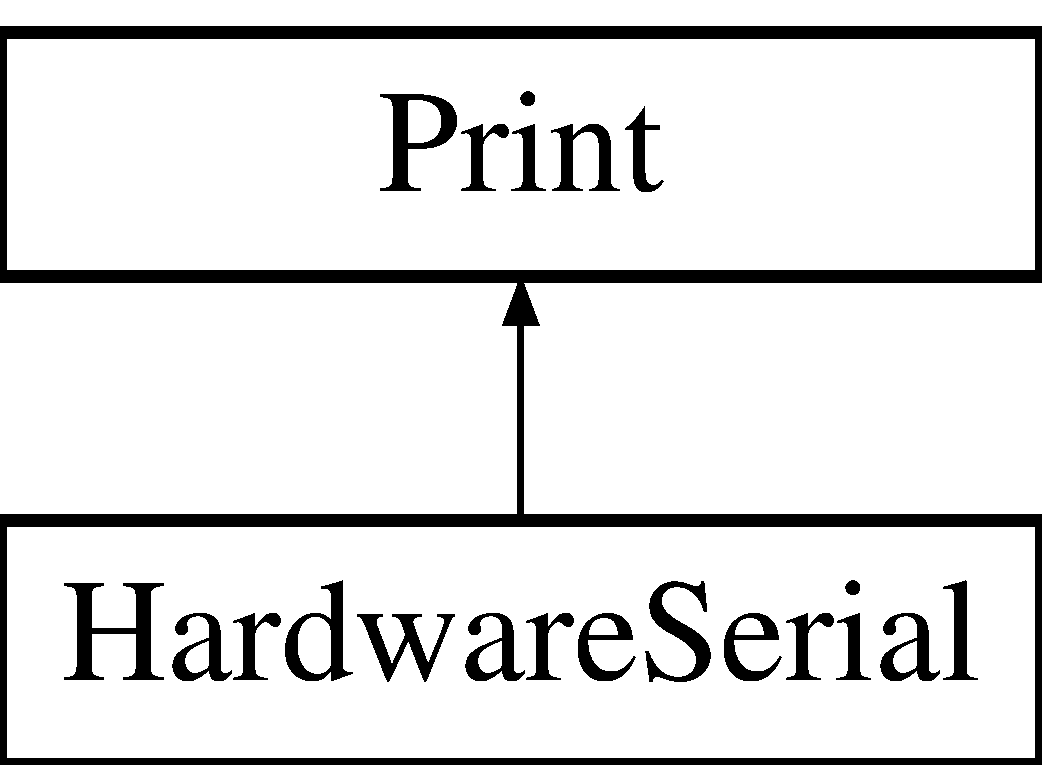
\includegraphics[height=2.000000cm]{class_hardware_serial}
\end{center}
\end{figure}
\subsubsection*{Public Member Functions}
\begin{DoxyCompactItemize}
\item 
\hyperlink{class_hardware_serial_ab96331f0886097eb802a7839676ef645}{HardwareSerial} (USART\_\-t $\ast$usart, PORT\_\-t $\ast$port, uint8\_\-t in\_\-bm, uint8\_\-t out\_\-bm)
\item 
\hyperlink{class_hardware_serial_a1c7aae049aba33b03fe030960c1c4aa7}{$\sim$HardwareSerial} ()
\item 
void \hyperlink{class_hardware_serial_a11049d350f4cf4bfdaafb24bb2738556}{begin} (long baudrate, int8\_\-t bscale=0)
\item 
void \hyperlink{class_hardware_serial_adcfab60db442174cb53f005df6d2996d}{begin2x} (long baudrate, int8\_\-t bscale=0)
\item 
void \hyperlink{class_hardware_serial_a0f86c41f580e04bdf30ea00e9014eacd}{end} ()
\item 
uint8\_\-t \hyperlink{class_hardware_serial_a10e05fa62dc473d0d8a7ee8184f504ba}{available} (void)
\item 
int \hyperlink{class_hardware_serial_a618696608a5fddcf3cb48ad6f044e756}{read} (void)
\item 
void \hyperlink{class_hardware_serial_a1eeb094d8da77e0292f95f4498a5396f}{flush} (void)
\item 
virtual void \hyperlink{class_hardware_serial_aced05ab99953383a235ccfb366f5c98f}{write} (uint8\_\-t)
\item 
void \hyperlink{class_hardware_serial_a2e13244413a84a259cadab3fb452921a}{enable} (bool bEn)
\end{DoxyCompactItemize}
\begin{Indent}{\bf Interrupt Handlers}\par
{\em There are three possible interrupts for the USART. Receive done, Transmit done and Data Register Ready. }\begin{DoxyCompactItemize}
\item 
void \hyperlink{class_hardware_serial_ac52002a727070c45b765d0dc55106cad}{rxc} ()
\item 
void \hyperlink{class_hardware_serial_ac33af9a86da3e3ae7ac1e2791c8eaf22}{dre} ()
\item 
void \hyperlink{class_hardware_serial_a82779b03507bc07f3bf2e090d3733015}{txc} ()
\end{DoxyCompactItemize}
\end{Indent}
\subsubsection*{Protected Attributes}
\begin{DoxyCompactItemize}
\item 
\hyperlink{structring__buffer}{ring\_\-buffer} $\ast$ \hyperlink{class_hardware_serial_a9ee5f8b61e049f98dfd0b5ae53e97273}{\_\-rx\_\-buffer}
\item 
USART\_\-t $\ast$ \hyperlink{class_hardware_serial_a3a3bd56aa561ae7e1eb1fd252b5b69a0}{\_\-usart}
\item 
PORT\_\-t $\ast$ \hyperlink{class_hardware_serial_add54c7d986c6122e8e8c23303f5b4845}{\_\-port}
\item 
uint8\_\-t \hyperlink{class_hardware_serial_a8724fdfd3955eeff5d3ed535624ce79a}{\_\-in\_\-bm}
\item 
uint8\_\-t \hyperlink{class_hardware_serial_a751a284e15af72b026143a8091be1b70}{\_\-out\_\-bm}
\item 
uint8\_\-t \hyperlink{class_hardware_serial_acc6c13c76a56c8b4bb88c3385b7bc791}{\_\-bsel}
\item 
int8\_\-t \hyperlink{class_hardware_serial_a37dd406c01fd6432618925f0aeb329f3}{\_\-bscale}
\item 
long \hyperlink{class_hardware_serial_ae692ab4a0a8aad73c74a10066fa9da24}{\_\-baudrate}
\item 
bool \hyperlink{class_hardware_serial_a8040fbab1f9197a9935df23a4c5e9a3b}{\_\-bEn}
\end{DoxyCompactItemize}


\subsubsection{Detailed Description}
\hyperlink{class_hardware_serial}{HardwareSerial} implementation. This class was originally copied form the Arduino source directory but has been modified somewhat to customize it for the CFA project.

Ths class wraps the hardware serial resource in the ATXmega The class handles an interupt driven receive with a fixed size receive buffer of 128 bytes. The current implementation uses a synchronous send, but a buffered send would be a great enhancement for performance purposes. 

Definition at line \hyperlink{_hardware_serial_8h_source_l00023}{23} of file \hyperlink{_hardware_serial_8h_source}{HardwareSerial.h}.



\subsubsection{Constructor \& Destructor Documentation}
\hypertarget{class_hardware_serial_ab96331f0886097eb802a7839676ef645}{
\index{HardwareSerial@{HardwareSerial}!HardwareSerial@{HardwareSerial}}
\index{HardwareSerial@{HardwareSerial}!HardwareSerial@{HardwareSerial}}
\paragraph[{HardwareSerial}]{\setlength{\rightskip}{0pt plus 5cm}HardwareSerial::HardwareSerial (
\begin{DoxyParamCaption}
\item[{USART\_\-t $\ast$}]{usart, }
\item[{PORT\_\-t $\ast$}]{port, }
\item[{uint8\_\-t}]{in\_\-bm, }
\item[{uint8\_\-t}]{out\_\-bm}
\end{DoxyParamCaption}
)}\hfill}
\label{class_hardware_serial_ab96331f0886097eb802a7839676ef645}


Definition at line \hyperlink{_hardware_serial_8cpp_source_l00112}{112} of file \hyperlink{_hardware_serial_8cpp_source}{HardwareSerial.cpp}.



References \hyperlink{_hardware_serial_8h_source_l00033}{\_\-baudrate}, \hyperlink{_hardware_serial_8h_source_l00034}{\_\-bEn}, \hyperlink{_hardware_serial_8h_source_l00032}{\_\-bscale}, \hyperlink{_hardware_serial_8h_source_l00031}{\_\-bsel}, \hyperlink{_hardware_serial_8h_source_l00029}{\_\-in\_\-bm}, \hyperlink{_hardware_serial_8h_source_l00030}{\_\-out\_\-bm}, \hyperlink{_hardware_serial_8h_source_l00028}{\_\-port}, \hyperlink{_hardware_serial_8h_source_l00026}{\_\-rx\_\-buffer}, \hyperlink{_hardware_serial_8h_source_l00027}{\_\-usart}, \hyperlink{_hardware_serial_8cpp_source_l00014}{RX\_\-BUFFER\_\-SIZE}, and \hyperlink{_hardware_serial_8cpp_source_l00061}{SetPointer()}.


\begin{DoxyCode}
\{
    \hyperlink{class_hardware_serial_a9ee5f8b61e049f98dfd0b5ae53e97273}{_rx_buffer} = (\hyperlink{structring__buffer}{ring_buffer}*)malloc(\hyperlink{_hardware_serial_8cpp_a739a2a1a0047c98ac1b18ecd25dac092}{RX_BUFFER_SIZE}+2*\textcolor{keyword}{sizeof}(\textcolor{keywordtype}{int}));
    \hyperlink{class_hardware_serial_a3a3bd56aa561ae7e1eb1fd252b5b69a0}{_usart}     = usart;
    \hyperlink{class_hardware_serial_add54c7d986c6122e8e8c23303f5b4845}{_port}      = port;
    \hyperlink{class_hardware_serial_a8724fdfd3955eeff5d3ed535624ce79a}{_in_bm}     = in\_bm;
    \hyperlink{class_hardware_serial_a751a284e15af72b026143a8091be1b70}{_out_bm}    = out\_bm;
    \hyperlink{class_hardware_serial_acc6c13c76a56c8b4bb88c3385b7bc791}{_bsel}      = 0;
    \hyperlink{class_hardware_serial_a37dd406c01fd6432618925f0aeb329f3}{_bscale}    = 0;
    \hyperlink{class_hardware_serial_ae692ab4a0a8aad73c74a10066fa9da24}{_baudrate}  = 9600;
    \hyperlink{class_hardware_serial_a8040fbab1f9197a9935df23a4c5e9a3b}{_bEn}       = \textcolor{keyword}{true};
    \hyperlink{_hardware_serial_8cpp_aaec4e4f887a958cc22dd447565d7080b}{SetPointer}(\hyperlink{class_hardware_serial_a3a3bd56aa561ae7e1eb1fd252b5b69a0}{_usart},\textcolor{keyword}{this});
\}
\end{DoxyCode}
\hypertarget{class_hardware_serial_a1c7aae049aba33b03fe030960c1c4aa7}{
\index{HardwareSerial@{HardwareSerial}!$\sim$HardwareSerial@{$\sim$HardwareSerial}}
\index{$\sim$HardwareSerial@{$\sim$HardwareSerial}!HardwareSerial@{HardwareSerial}}
\paragraph[{$\sim$HardwareSerial}]{\setlength{\rightskip}{0pt plus 5cm}HardwareSerial::$\sim$HardwareSerial (
\begin{DoxyParamCaption}
{}
\end{DoxyParamCaption}
)}\hfill}
\label{class_hardware_serial_a1c7aae049aba33b03fe030960c1c4aa7}


Definition at line \hyperlink{_hardware_serial_8cpp_source_l00130}{130} of file \hyperlink{_hardware_serial_8cpp_source}{HardwareSerial.cpp}.



References \hyperlink{_hardware_serial_8h_source_l00026}{\_\-rx\_\-buffer}, \hyperlink{_hardware_serial_8h_source_l00027}{\_\-usart}, \hyperlink{_hardware_serial_8cpp_source_l00203}{end()}, and \hyperlink{_hardware_serial_8cpp_source_l00061}{SetPointer()}.


\begin{DoxyCode}
\{
    \hyperlink{class_hardware_serial_a0f86c41f580e04bdf30ea00e9014eacd}{end}();
    free(\hyperlink{class_hardware_serial_a9ee5f8b61e049f98dfd0b5ae53e97273}{_rx_buffer});
    \hyperlink{class_hardware_serial_a9ee5f8b61e049f98dfd0b5ae53e97273}{_rx_buffer} = 0;
    \hyperlink{_hardware_serial_8cpp_aaec4e4f887a958cc22dd447565d7080b}{SetPointer}(\hyperlink{class_hardware_serial_a3a3bd56aa561ae7e1eb1fd252b5b69a0}{_usart},0);
\}
\end{DoxyCode}


\subsubsection{Member Function Documentation}
\hypertarget{class_hardware_serial_a10e05fa62dc473d0d8a7ee8184f504ba}{
\index{HardwareSerial@{HardwareSerial}!available@{available}}
\index{available@{available}!HardwareSerial@{HardwareSerial}}
\paragraph[{available}]{\setlength{\rightskip}{0pt plus 5cm}uint8\_\-t HardwareSerial::available (
\begin{DoxyParamCaption}
\item[{void}]{}
\end{DoxyParamCaption}
)}\hfill}
\label{class_hardware_serial_a10e05fa62dc473d0d8a7ee8184f504ba}


Definition at line \hyperlink{_hardware_serial_8cpp_source_l00213}{213} of file \hyperlink{_hardware_serial_8cpp_source}{HardwareSerial.cpp}.



References \hyperlink{_hardware_serial_8h_source_l00026}{\_\-rx\_\-buffer}, \hyperlink{_hardware_serial_8cpp_source_l00018}{ring\_\-buffer::head}, \hyperlink{_hardware_serial_8cpp_source_l00014}{RX\_\-BUFFER\_\-SIZE}, and \hyperlink{_hardware_serial_8cpp_source_l00019}{ring\_\-buffer::tail}.



Referenced by \hyperlink{_cmd_processor_8cpp_source_l00068}{CmdProcessor::checkCommands()}.


\begin{DoxyCode}
\{
    \textcolor{keywordflow}{return} (\hyperlink{_hardware_serial_8cpp_a739a2a1a0047c98ac1b18ecd25dac092}{RX_BUFFER_SIZE} + \hyperlink{class_hardware_serial_a9ee5f8b61e049f98dfd0b5ae53e97273}{_rx_buffer}->\hyperlink{structring__buffer_ac1b620f2e27c3af75e68bd1645a2f5f0}{head} - \hyperlink{class_hardware_serial_a9ee5f8b61e049f98dfd0b5ae53e97273}{_rx_buffer}->\hyperlink{structring__buffer_a4d06965736f37f64f15bbd0ca9457771}{tail}) % 
      \hyperlink{_hardware_serial_8cpp_a739a2a1a0047c98ac1b18ecd25dac092}{RX_BUFFER_SIZE};
\}
\end{DoxyCode}
\hypertarget{class_hardware_serial_a11049d350f4cf4bfdaafb24bb2738556}{
\index{HardwareSerial@{HardwareSerial}!begin@{begin}}
\index{begin@{begin}!HardwareSerial@{HardwareSerial}}
\paragraph[{begin}]{\setlength{\rightskip}{0pt plus 5cm}void HardwareSerial::begin (
\begin{DoxyParamCaption}
\item[{long}]{baudrate, }
\item[{int8\_\-t}]{bscale = {\ttfamily 0}}
\end{DoxyParamCaption}
)}\hfill}
\label{class_hardware_serial_a11049d350f4cf4bfdaafb24bb2738556}


Definition at line \hyperlink{_hardware_serial_8cpp_source_l00140}{140} of file \hyperlink{_hardware_serial_8cpp_source}{HardwareSerial.cpp}.



References \hyperlink{_hardware_serial_8h_source_l00033}{\_\-baudrate}, \hyperlink{_hardware_serial_8h_source_l00032}{\_\-bscale}, \hyperlink{_hardware_serial_8h_source_l00029}{\_\-in\_\-bm}, \hyperlink{_hardware_serial_8h_source_l00030}{\_\-out\_\-bm}, \hyperlink{_hardware_serial_8h_source_l00028}{\_\-port}, and \hyperlink{_hardware_serial_8h_source_l00027}{\_\-usart}.



Referenced by \hyperlink{_gyro_acc_8cpp_source_l00034}{main()}.


\begin{DoxyCode}
\{
    uint16\_t BSEL;
    \hyperlink{class_hardware_serial_a37dd406c01fd6432618925f0aeb329f3}{_bscale} = bscale;
    \hyperlink{class_hardware_serial_ae692ab4a0a8aad73c74a10066fa9da24}{_baudrate} = baud;
    
    \textcolor{keywordtype}{float} fPER = F\_CPU;
    \textcolor{keywordtype}{float} fBaud = baud;
    
    \hyperlink{class_hardware_serial_add54c7d986c6122e8e8c23303f5b4845}{_port}->DIRCLR = \hyperlink{class_hardware_serial_a8724fdfd3955eeff5d3ed535624ce79a}{_in_bm};  \textcolor{comment}{// input}
    \hyperlink{class_hardware_serial_add54c7d986c6122e8e8c23303f5b4845}{_port}->DIRSET = \hyperlink{class_hardware_serial_a751a284e15af72b026143a8091be1b70}{_out_bm}; \textcolor{comment}{// output}
    
    \textcolor{comment}{// set the baud rate}
    \textcolor{keywordflow}{if} (bscale >= 0) \{
        BSEL = fPER/((1 << bscale) * 16 * baud) - 1;
        \textcolor{comment}{//BSEL = F\_CPU / 16 / baud - 1;}
    \} \textcolor{keywordflow}{else} \{
        bscale = -1 * bscale;
        BSEL = (1 << bscale) * (fPER/(16.0 * fBaud) - 1);
    \}
    
    \hyperlink{class_hardware_serial_a3a3bd56aa561ae7e1eb1fd252b5b69a0}{_usart}->BAUDCTRLA = (uint8\_t)BSEL;
    \hyperlink{class_hardware_serial_a3a3bd56aa561ae7e1eb1fd252b5b69a0}{_usart}->BAUDCTRLB = ((bscale & 0xf) << 4) | ((BSEL & 0xf00) >> 8);
    
    \textcolor{comment}{// enable Rx and Tx}
    \hyperlink{class_hardware_serial_a3a3bd56aa561ae7e1eb1fd252b5b69a0}{_usart}->CTRLB |= USART\_RXEN\_bm | USART\_TXEN\_bm;
    \textcolor{comment}{// enable interrupt}
    \hyperlink{class_hardware_serial_a3a3bd56aa561ae7e1eb1fd252b5b69a0}{_usart}->CTRLA = USART\_RXCINTLVL\_HI\_gc;
    
    \textcolor{comment}{// Char size, parity and stop bits: 8N1}
    \hyperlink{class_hardware_serial_a3a3bd56aa561ae7e1eb1fd252b5b69a0}{_usart}->CTRLC = USART\_CHSIZE\_8BIT\_gc | USART\_PMODE\_DISABLED\_gc;
\}
\end{DoxyCode}
\hypertarget{class_hardware_serial_adcfab60db442174cb53f005df6d2996d}{
\index{HardwareSerial@{HardwareSerial}!begin2x@{begin2x}}
\index{begin2x@{begin2x}!HardwareSerial@{HardwareSerial}}
\paragraph[{begin2x}]{\setlength{\rightskip}{0pt plus 5cm}void HardwareSerial::begin2x (
\begin{DoxyParamCaption}
\item[{long}]{baudrate, }
\item[{int8\_\-t}]{bscale = {\ttfamily 0}}
\end{DoxyParamCaption}
)}\hfill}
\label{class_hardware_serial_adcfab60db442174cb53f005df6d2996d}


Definition at line \hyperlink{_hardware_serial_8cpp_source_l00173}{173} of file \hyperlink{_hardware_serial_8cpp_source}{HardwareSerial.cpp}.



References \hyperlink{_hardware_serial_8h_source_l00033}{\_\-baudrate}, \hyperlink{_hardware_serial_8h_source_l00032}{\_\-bscale}, \hyperlink{_hardware_serial_8h_source_l00029}{\_\-in\_\-bm}, \hyperlink{_hardware_serial_8h_source_l00030}{\_\-out\_\-bm}, \hyperlink{_hardware_serial_8h_source_l00028}{\_\-port}, \hyperlink{_hardware_serial_8h_source_l00027}{\_\-usart}, and \hyperlink{_hardware_serial_8cpp_source_l00061}{SetPointer()}.


\begin{DoxyCode}
\{
    uint16\_t baud\_setting;
    \hyperlink{class_hardware_serial_a37dd406c01fd6432618925f0aeb329f3}{_bscale} = bscale;
    \hyperlink{class_hardware_serial_ae692ab4a0a8aad73c74a10066fa9da24}{_baudrate} = baud;
    
    \textcolor{comment}{// TODO: Serial. Fix serial double clock.}
    \textcolor{keywordtype}{long} fPER = F\_CPU * 4;
    
    \hyperlink{class_hardware_serial_add54c7d986c6122e8e8c23303f5b4845}{_port}->DIRCLR = \hyperlink{class_hardware_serial_a8724fdfd3955eeff5d3ed535624ce79a}{_in_bm};  \textcolor{comment}{// input}
    \hyperlink{class_hardware_serial_add54c7d986c6122e8e8c23303f5b4845}{_port}->DIRSET = \hyperlink{class_hardware_serial_a751a284e15af72b026143a8091be1b70}{_out_bm}; \textcolor{comment}{// output}
    
    \textcolor{comment}{// set the baud rate using the 2X calculations}
    \hyperlink{class_hardware_serial_a3a3bd56aa561ae7e1eb1fd252b5b69a0}{_usart}->CTRLB |= 1 << 1; \textcolor{comment}{// the last 1 was the \_u2x value}
    baud\_setting = fPER / 8 / baud - 1;

    \hyperlink{class_hardware_serial_a3a3bd56aa561ae7e1eb1fd252b5b69a0}{_usart}->BAUDCTRLA = (uint8\_t)baud\_setting;
    \hyperlink{class_hardware_serial_a3a3bd56aa561ae7e1eb1fd252b5b69a0}{_usart}->BAUDCTRLB = baud\_setting >> 8;
    
    
    \textcolor{comment}{// enable Rx and Tx}
    \hyperlink{class_hardware_serial_a3a3bd56aa561ae7e1eb1fd252b5b69a0}{_usart}->CTRLB |= USART\_RXEN\_bm | USART\_TXEN\_bm;
    \textcolor{comment}{// enable interrupt}
    \hyperlink{class_hardware_serial_a3a3bd56aa561ae7e1eb1fd252b5b69a0}{_usart}->CTRLA = (\hyperlink{class_hardware_serial_a3a3bd56aa561ae7e1eb1fd252b5b69a0}{_usart}->CTRLA & ~USART\_RXCINTLVL\_gm) | USART\_RXCINTLVL\_LO\_gc
      ;
    
    \textcolor{comment}{// Char size, parity and stop bits: 8N1}
    \hyperlink{class_hardware_serial_a3a3bd56aa561ae7e1eb1fd252b5b69a0}{_usart}->CTRLC = USART\_CHSIZE\_8BIT\_gc | USART\_PMODE\_DISABLED\_gc;
    \hyperlink{_hardware_serial_8cpp_aaec4e4f887a958cc22dd447565d7080b}{SetPointer}(\hyperlink{class_hardware_serial_a3a3bd56aa561ae7e1eb1fd252b5b69a0}{_usart},\textcolor{keyword}{this});
\}
\end{DoxyCode}
\hypertarget{class_hardware_serial_ac33af9a86da3e3ae7ac1e2791c8eaf22}{
\index{HardwareSerial@{HardwareSerial}!dre@{dre}}
\index{dre@{dre}!HardwareSerial@{HardwareSerial}}
\paragraph[{dre}]{\setlength{\rightskip}{0pt plus 5cm}void HardwareSerial::dre (
\begin{DoxyParamCaption}
{}
\end{DoxyParamCaption}
)}\hfill}
\label{class_hardware_serial_ac33af9a86da3e3ae7ac1e2791c8eaf22}


Definition at line \hyperlink{_hardware_serial_8cpp_source_l00100}{100} of file \hyperlink{_hardware_serial_8cpp_source}{HardwareSerial.cpp}.


\begin{DoxyCode}
\{
\}
\end{DoxyCode}
\hypertarget{class_hardware_serial_a2e13244413a84a259cadab3fb452921a}{
\index{HardwareSerial@{HardwareSerial}!enable@{enable}}
\index{enable@{enable}!HardwareSerial@{HardwareSerial}}
\paragraph[{enable}]{\setlength{\rightskip}{0pt plus 5cm}void HardwareSerial::enable (
\begin{DoxyParamCaption}
\item[{bool}]{bEn}
\end{DoxyParamCaption}
)}\hfill}
\label{class_hardware_serial_a2e13244413a84a259cadab3fb452921a}


Definition at line \hyperlink{_hardware_serial_8cpp_source_l00248}{248} of file \hyperlink{_hardware_serial_8cpp_source}{HardwareSerial.cpp}.



References \hyperlink{_hardware_serial_8h_source_l00034}{\_\-bEn}.



Referenced by \hyperlink{_gyro_acc_8cpp_source_l00034}{main()}.


\begin{DoxyCode}
\{
    \hyperlink{class_hardware_serial_a8040fbab1f9197a9935df23a4c5e9a3b}{_bEn} = bEn;
\}
\end{DoxyCode}
\hypertarget{class_hardware_serial_a0f86c41f580e04bdf30ea00e9014eacd}{
\index{HardwareSerial@{HardwareSerial}!end@{end}}
\index{end@{end}!HardwareSerial@{HardwareSerial}}
\paragraph[{end}]{\setlength{\rightskip}{0pt plus 5cm}void HardwareSerial::end (
\begin{DoxyParamCaption}
{}
\end{DoxyParamCaption}
)}\hfill}
\label{class_hardware_serial_a0f86c41f580e04bdf30ea00e9014eacd}


Definition at line \hyperlink{_hardware_serial_8cpp_source_l00203}{203} of file \hyperlink{_hardware_serial_8cpp_source}{HardwareSerial.cpp}.



References \hyperlink{_hardware_serial_8h_source_l00027}{\_\-usart}, and \hyperlink{_hardware_serial_8cpp_source_l00061}{SetPointer()}.



Referenced by \hyperlink{_cmd_processor_8cpp_source_l00025}{CmdProcessor::$\sim$CmdProcessor()}, and \hyperlink{_hardware_serial_8cpp_source_l00130}{$\sim$HardwareSerial()}.


\begin{DoxyCode}
\{
    \hyperlink{_hardware_serial_8cpp_aaec4e4f887a958cc22dd447565d7080b}{SetPointer}(\hyperlink{class_hardware_serial_a3a3bd56aa561ae7e1eb1fd252b5b69a0}{_usart},(\hyperlink{class_hardware_serial}{HardwareSerial}*)0);
    
    \textcolor{comment}{// disable Rx and Tx}
    \hyperlink{class_hardware_serial_a3a3bd56aa561ae7e1eb1fd252b5b69a0}{_usart}->CTRLB &= ~(USART\_RXEN\_bm | USART\_TXEN\_bm);
    \textcolor{comment}{// disable interrupt}
    \hyperlink{class_hardware_serial_a3a3bd56aa561ae7e1eb1fd252b5b69a0}{_usart}->CTRLA = (\hyperlink{class_hardware_serial_a3a3bd56aa561ae7e1eb1fd252b5b69a0}{_usart}->CTRLA & ~USART\_RXCINTLVL\_gm) | USART\_RXCINTLVL\_LO\_gc
      ;
\}
\end{DoxyCode}
\hypertarget{class_hardware_serial_a1eeb094d8da77e0292f95f4498a5396f}{
\index{HardwareSerial@{HardwareSerial}!flush@{flush}}
\index{flush@{flush}!HardwareSerial@{HardwareSerial}}
\paragraph[{flush}]{\setlength{\rightskip}{0pt plus 5cm}void HardwareSerial::flush (
\begin{DoxyParamCaption}
\item[{void}]{}
\end{DoxyParamCaption}
)}\hfill}
\label{class_hardware_serial_a1eeb094d8da77e0292f95f4498a5396f}


Definition at line \hyperlink{_hardware_serial_8cpp_source_l00230}{230} of file \hyperlink{_hardware_serial_8cpp_source}{HardwareSerial.cpp}.



References \hyperlink{_hardware_serial_8h_source_l00026}{\_\-rx\_\-buffer}, \hyperlink{_hardware_serial_8cpp_source_l00018}{ring\_\-buffer::head}, and \hyperlink{_hardware_serial_8cpp_source_l00019}{ring\_\-buffer::tail}.


\begin{DoxyCode}
\{
    \textcolor{comment}{// don't reverse this or there may be problems if the RX interrupt}
    \textcolor{comment}{// occurs after reading the value of rx\_buffer\_head but before writing}
    \textcolor{comment}{// the value to rx\_buffer\_tail; the previous value of rx\_buffer\_head}
    \textcolor{comment}{// may be written to rx\_buffer\_tail, making it appear as if the buffer}
    \textcolor{comment}{// were full, not empty.}
    \hyperlink{class_hardware_serial_a9ee5f8b61e049f98dfd0b5ae53e97273}{_rx_buffer}->\hyperlink{structring__buffer_ac1b620f2e27c3af75e68bd1645a2f5f0}{head} = \hyperlink{class_hardware_serial_a9ee5f8b61e049f98dfd0b5ae53e97273}{_rx_buffer}->\hyperlink{structring__buffer_a4d06965736f37f64f15bbd0ca9457771}{tail};
\}
\end{DoxyCode}
\hypertarget{class_hardware_serial_a618696608a5fddcf3cb48ad6f044e756}{
\index{HardwareSerial@{HardwareSerial}!read@{read}}
\index{read@{read}!HardwareSerial@{HardwareSerial}}
\paragraph[{read}]{\setlength{\rightskip}{0pt plus 5cm}int HardwareSerial::read (
\begin{DoxyParamCaption}
\item[{void}]{}
\end{DoxyParamCaption}
)}\hfill}
\label{class_hardware_serial_a618696608a5fddcf3cb48ad6f044e756}


Definition at line \hyperlink{_hardware_serial_8cpp_source_l00218}{218} of file \hyperlink{_hardware_serial_8cpp_source}{HardwareSerial.cpp}.



References \hyperlink{_hardware_serial_8h_source_l00026}{\_\-rx\_\-buffer}, \hyperlink{_hardware_serial_8cpp_source_l00017}{ring\_\-buffer::buffer}, \hyperlink{_hardware_serial_8cpp_source_l00018}{ring\_\-buffer::head}, \hyperlink{_hardware_serial_8cpp_source_l00014}{RX\_\-BUFFER\_\-SIZE}, and \hyperlink{_hardware_serial_8cpp_source_l00019}{ring\_\-buffer::tail}.



Referenced by \hyperlink{_cmd_processor_8cpp_source_l00068}{CmdProcessor::checkCommands()}.


\begin{DoxyCode}
\{
    \textcolor{comment}{// if the head isn't ahead of the tail, we don't have any characters}
    \textcolor{keywordflow}{if} (\hyperlink{class_hardware_serial_a9ee5f8b61e049f98dfd0b5ae53e97273}{_rx_buffer}->\hyperlink{structring__buffer_ac1b620f2e27c3af75e68bd1645a2f5f0}{head} == \hyperlink{class_hardware_serial_a9ee5f8b61e049f98dfd0b5ae53e97273}{_rx_buffer}->\hyperlink{structring__buffer_a4d06965736f37f64f15bbd0ca9457771}{tail}) \{
        \textcolor{keywordflow}{return} -1;
    \} \textcolor{keywordflow}{else} \{
        \textcolor{keywordtype}{unsigned} \textcolor{keywordtype}{char} c = \hyperlink{class_hardware_serial_a9ee5f8b61e049f98dfd0b5ae53e97273}{_rx_buffer}->\hyperlink{structring__buffer_a11b70d4a150ea9750e4102706d6ee0b8}{buffer}[\hyperlink{class_hardware_serial_a9ee5f8b61e049f98dfd0b5ae53e97273}{_rx_buffer}->\hyperlink{structring__buffer_a4d06965736f37f64f15bbd0ca9457771}{tail}];
        \hyperlink{class_hardware_serial_a9ee5f8b61e049f98dfd0b5ae53e97273}{_rx_buffer}->\hyperlink{structring__buffer_a4d06965736f37f64f15bbd0ca9457771}{tail} = (\hyperlink{class_hardware_serial_a9ee5f8b61e049f98dfd0b5ae53e97273}{_rx_buffer}->\hyperlink{structring__buffer_a4d06965736f37f64f15bbd0ca9457771}{tail} + 1) % \hyperlink{_hardware_serial_8cpp_a739a2a1a0047c98ac1b18ecd25dac092}{RX_BUFFER_SIZE};
        \textcolor{keywordflow}{return} c;
    \}
\}
\end{DoxyCode}
\hypertarget{class_hardware_serial_ac52002a727070c45b765d0dc55106cad}{
\index{HardwareSerial@{HardwareSerial}!rxc@{rxc}}
\index{rxc@{rxc}!HardwareSerial@{HardwareSerial}}
\paragraph[{rxc}]{\setlength{\rightskip}{0pt plus 5cm}void HardwareSerial::rxc (
\begin{DoxyParamCaption}
{}
\end{DoxyParamCaption}
)}\hfill}
\label{class_hardware_serial_ac52002a727070c45b765d0dc55106cad}


Definition at line \hyperlink{_hardware_serial_8cpp_source_l00094}{94} of file \hyperlink{_hardware_serial_8cpp_source}{HardwareSerial.cpp}.



References \hyperlink{_hardware_serial_8h_source_l00026}{\_\-rx\_\-buffer}, \hyperlink{_hardware_serial_8h_source_l00027}{\_\-usart}, and \hyperlink{_hardware_serial_8cpp_source_l00047}{store\_\-char()}.


\begin{DoxyCode}
\{
    \textcolor{keywordtype}{unsigned} \textcolor{keywordtype}{char} c = \hyperlink{class_hardware_serial_a3a3bd56aa561ae7e1eb1fd252b5b69a0}{_usart}->DATA;
    \hyperlink{_hardware_serial_8cpp_ac661d0ebc0efa48a2b2aed9ccf86aa64}{store_char}(c,\hyperlink{class_hardware_serial_a9ee5f8b61e049f98dfd0b5ae53e97273}{_rx_buffer});
\}
\end{DoxyCode}
\hypertarget{class_hardware_serial_a82779b03507bc07f3bf2e090d3733015}{
\index{HardwareSerial@{HardwareSerial}!txc@{txc}}
\index{txc@{txc}!HardwareSerial@{HardwareSerial}}
\paragraph[{txc}]{\setlength{\rightskip}{0pt plus 5cm}void HardwareSerial::txc (
\begin{DoxyParamCaption}
{}
\end{DoxyParamCaption}
)}\hfill}
\label{class_hardware_serial_a82779b03507bc07f3bf2e090d3733015}


Definition at line \hyperlink{_hardware_serial_8cpp_source_l00104}{104} of file \hyperlink{_hardware_serial_8cpp_source}{HardwareSerial.cpp}.


\begin{DoxyCode}
\{
\}
\end{DoxyCode}
\hypertarget{class_hardware_serial_aced05ab99953383a235ccfb366f5c98f}{
\index{HardwareSerial@{HardwareSerial}!write@{write}}
\index{write@{write}!HardwareSerial@{HardwareSerial}}
\paragraph[{write}]{\setlength{\rightskip}{0pt plus 5cm}void HardwareSerial::write (
\begin{DoxyParamCaption}
\item[{uint8\_\-t}]{c}
\end{DoxyParamCaption}
)\hspace{0.3cm}{\ttfamily  \mbox{[}virtual\mbox{]}}}\hfill}
\label{class_hardware_serial_aced05ab99953383a235ccfb366f5c98f}


Implements \hyperlink{class_print_ad9393033793cfc17f3e37202ba244892}{Print}.



Definition at line \hyperlink{_hardware_serial_8cpp_source_l00240}{240} of file \hyperlink{_hardware_serial_8cpp_source}{HardwareSerial.cpp}.



References \hyperlink{_hardware_serial_8h_source_l00034}{\_\-bEn}, and \hyperlink{_hardware_serial_8h_source_l00027}{\_\-usart}.


\begin{DoxyCode}
\{
    \textcolor{keywordflow}{if} (\hyperlink{class_hardware_serial_a8040fbab1f9197a9935df23a4c5e9a3b}{_bEn}) \{
        \textcolor{keywordflow}{while} ( !(\hyperlink{class_hardware_serial_a3a3bd56aa561ae7e1eb1fd252b5b69a0}{_usart}->STATUS & USART\_DREIF\_bm) );
        \hyperlink{class_hardware_serial_a3a3bd56aa561ae7e1eb1fd252b5b69a0}{_usart}->DATA = c;
    \}
\}
\end{DoxyCode}


\subsubsection{Member Data Documentation}
\hypertarget{class_hardware_serial_ae692ab4a0a8aad73c74a10066fa9da24}{
\index{HardwareSerial@{HardwareSerial}!\_\-baudrate@{\_\-baudrate}}
\index{\_\-baudrate@{\_\-baudrate}!HardwareSerial@{HardwareSerial}}
\paragraph[{\_\-baudrate}]{\setlength{\rightskip}{0pt plus 5cm}long {\bf HardwareSerial::\_\-baudrate}\hspace{0.3cm}{\ttfamily  \mbox{[}protected\mbox{]}}}\hfill}
\label{class_hardware_serial_ae692ab4a0a8aad73c74a10066fa9da24}


Definition at line \hyperlink{_hardware_serial_8h_source_l00033}{33} of file \hyperlink{_hardware_serial_8h_source}{HardwareSerial.h}.



Referenced by \hyperlink{_hardware_serial_8cpp_source_l00140}{begin()}, \hyperlink{_hardware_serial_8cpp_source_l00173}{begin2x()}, and \hyperlink{_hardware_serial_8cpp_source_l00112}{HardwareSerial()}.

\hypertarget{class_hardware_serial_a8040fbab1f9197a9935df23a4c5e9a3b}{
\index{HardwareSerial@{HardwareSerial}!\_\-bEn@{\_\-bEn}}
\index{\_\-bEn@{\_\-bEn}!HardwareSerial@{HardwareSerial}}
\paragraph[{\_\-bEn}]{\setlength{\rightskip}{0pt plus 5cm}bool {\bf HardwareSerial::\_\-bEn}\hspace{0.3cm}{\ttfamily  \mbox{[}protected\mbox{]}}}\hfill}
\label{class_hardware_serial_a8040fbab1f9197a9935df23a4c5e9a3b}


Definition at line \hyperlink{_hardware_serial_8h_source_l00034}{34} of file \hyperlink{_hardware_serial_8h_source}{HardwareSerial.h}.



Referenced by \hyperlink{_hardware_serial_8cpp_source_l00248}{enable()}, \hyperlink{_hardware_serial_8cpp_source_l00112}{HardwareSerial()}, and \hyperlink{_hardware_serial_8cpp_source_l00240}{write()}.

\hypertarget{class_hardware_serial_a37dd406c01fd6432618925f0aeb329f3}{
\index{HardwareSerial@{HardwareSerial}!\_\-bscale@{\_\-bscale}}
\index{\_\-bscale@{\_\-bscale}!HardwareSerial@{HardwareSerial}}
\paragraph[{\_\-bscale}]{\setlength{\rightskip}{0pt plus 5cm}int8\_\-t {\bf HardwareSerial::\_\-bscale}\hspace{0.3cm}{\ttfamily  \mbox{[}protected\mbox{]}}}\hfill}
\label{class_hardware_serial_a37dd406c01fd6432618925f0aeb329f3}


Definition at line \hyperlink{_hardware_serial_8h_source_l00032}{32} of file \hyperlink{_hardware_serial_8h_source}{HardwareSerial.h}.



Referenced by \hyperlink{_hardware_serial_8cpp_source_l00140}{begin()}, \hyperlink{_hardware_serial_8cpp_source_l00173}{begin2x()}, and \hyperlink{_hardware_serial_8cpp_source_l00112}{HardwareSerial()}.

\hypertarget{class_hardware_serial_acc6c13c76a56c8b4bb88c3385b7bc791}{
\index{HardwareSerial@{HardwareSerial}!\_\-bsel@{\_\-bsel}}
\index{\_\-bsel@{\_\-bsel}!HardwareSerial@{HardwareSerial}}
\paragraph[{\_\-bsel}]{\setlength{\rightskip}{0pt plus 5cm}uint8\_\-t {\bf HardwareSerial::\_\-bsel}\hspace{0.3cm}{\ttfamily  \mbox{[}protected\mbox{]}}}\hfill}
\label{class_hardware_serial_acc6c13c76a56c8b4bb88c3385b7bc791}


Definition at line \hyperlink{_hardware_serial_8h_source_l00031}{31} of file \hyperlink{_hardware_serial_8h_source}{HardwareSerial.h}.



Referenced by \hyperlink{_hardware_serial_8cpp_source_l00112}{HardwareSerial()}.

\hypertarget{class_hardware_serial_a8724fdfd3955eeff5d3ed535624ce79a}{
\index{HardwareSerial@{HardwareSerial}!\_\-in\_\-bm@{\_\-in\_\-bm}}
\index{\_\-in\_\-bm@{\_\-in\_\-bm}!HardwareSerial@{HardwareSerial}}
\paragraph[{\_\-in\_\-bm}]{\setlength{\rightskip}{0pt plus 5cm}uint8\_\-t {\bf HardwareSerial::\_\-in\_\-bm}\hspace{0.3cm}{\ttfamily  \mbox{[}protected\mbox{]}}}\hfill}
\label{class_hardware_serial_a8724fdfd3955eeff5d3ed535624ce79a}


Definition at line \hyperlink{_hardware_serial_8h_source_l00029}{29} of file \hyperlink{_hardware_serial_8h_source}{HardwareSerial.h}.



Referenced by \hyperlink{_hardware_serial_8cpp_source_l00140}{begin()}, \hyperlink{_hardware_serial_8cpp_source_l00173}{begin2x()}, and \hyperlink{_hardware_serial_8cpp_source_l00112}{HardwareSerial()}.

\hypertarget{class_hardware_serial_a751a284e15af72b026143a8091be1b70}{
\index{HardwareSerial@{HardwareSerial}!\_\-out\_\-bm@{\_\-out\_\-bm}}
\index{\_\-out\_\-bm@{\_\-out\_\-bm}!HardwareSerial@{HardwareSerial}}
\paragraph[{\_\-out\_\-bm}]{\setlength{\rightskip}{0pt plus 5cm}uint8\_\-t {\bf HardwareSerial::\_\-out\_\-bm}\hspace{0.3cm}{\ttfamily  \mbox{[}protected\mbox{]}}}\hfill}
\label{class_hardware_serial_a751a284e15af72b026143a8091be1b70}


Definition at line \hyperlink{_hardware_serial_8h_source_l00030}{30} of file \hyperlink{_hardware_serial_8h_source}{HardwareSerial.h}.



Referenced by \hyperlink{_hardware_serial_8cpp_source_l00140}{begin()}, \hyperlink{_hardware_serial_8cpp_source_l00173}{begin2x()}, and \hyperlink{_hardware_serial_8cpp_source_l00112}{HardwareSerial()}.

\hypertarget{class_hardware_serial_add54c7d986c6122e8e8c23303f5b4845}{
\index{HardwareSerial@{HardwareSerial}!\_\-port@{\_\-port}}
\index{\_\-port@{\_\-port}!HardwareSerial@{HardwareSerial}}
\paragraph[{\_\-port}]{\setlength{\rightskip}{0pt plus 5cm}PORT\_\-t$\ast$ {\bf HardwareSerial::\_\-port}\hspace{0.3cm}{\ttfamily  \mbox{[}protected\mbox{]}}}\hfill}
\label{class_hardware_serial_add54c7d986c6122e8e8c23303f5b4845}


Definition at line \hyperlink{_hardware_serial_8h_source_l00028}{28} of file \hyperlink{_hardware_serial_8h_source}{HardwareSerial.h}.



Referenced by \hyperlink{_hardware_serial_8cpp_source_l00140}{begin()}, \hyperlink{_hardware_serial_8cpp_source_l00173}{begin2x()}, and \hyperlink{_hardware_serial_8cpp_source_l00112}{HardwareSerial()}.

\hypertarget{class_hardware_serial_a9ee5f8b61e049f98dfd0b5ae53e97273}{
\index{HardwareSerial@{HardwareSerial}!\_\-rx\_\-buffer@{\_\-rx\_\-buffer}}
\index{\_\-rx\_\-buffer@{\_\-rx\_\-buffer}!HardwareSerial@{HardwareSerial}}
\paragraph[{\_\-rx\_\-buffer}]{\setlength{\rightskip}{0pt plus 5cm}{\bf ring\_\-buffer}$\ast$ {\bf HardwareSerial::\_\-rx\_\-buffer}\hspace{0.3cm}{\ttfamily  \mbox{[}protected\mbox{]}}}\hfill}
\label{class_hardware_serial_a9ee5f8b61e049f98dfd0b5ae53e97273}


Definition at line \hyperlink{_hardware_serial_8h_source_l00026}{26} of file \hyperlink{_hardware_serial_8h_source}{HardwareSerial.h}.



Referenced by \hyperlink{_hardware_serial_8cpp_source_l00213}{available()}, \hyperlink{_hardware_serial_8cpp_source_l00230}{flush()}, \hyperlink{_hardware_serial_8cpp_source_l00112}{HardwareSerial()}, \hyperlink{_hardware_serial_8cpp_source_l00218}{read()}, \hyperlink{_hardware_serial_8cpp_source_l00094}{rxc()}, and \hyperlink{_hardware_serial_8cpp_source_l00130}{$\sim$HardwareSerial()}.

\hypertarget{class_hardware_serial_a3a3bd56aa561ae7e1eb1fd252b5b69a0}{
\index{HardwareSerial@{HardwareSerial}!\_\-usart@{\_\-usart}}
\index{\_\-usart@{\_\-usart}!HardwareSerial@{HardwareSerial}}
\paragraph[{\_\-usart}]{\setlength{\rightskip}{0pt plus 5cm}USART\_\-t$\ast$ {\bf HardwareSerial::\_\-usart}\hspace{0.3cm}{\ttfamily  \mbox{[}protected\mbox{]}}}\hfill}
\label{class_hardware_serial_a3a3bd56aa561ae7e1eb1fd252b5b69a0}


Definition at line \hyperlink{_hardware_serial_8h_source_l00027}{27} of file \hyperlink{_hardware_serial_8h_source}{HardwareSerial.h}.



Referenced by \hyperlink{_hardware_serial_8cpp_source_l00140}{begin()}, \hyperlink{_hardware_serial_8cpp_source_l00173}{begin2x()}, \hyperlink{_hardware_serial_8cpp_source_l00203}{end()}, \hyperlink{_hardware_serial_8cpp_source_l00112}{HardwareSerial()}, \hyperlink{_hardware_serial_8cpp_source_l00094}{rxc()}, \hyperlink{_hardware_serial_8cpp_source_l00240}{write()}, and \hyperlink{_hardware_serial_8cpp_source_l00130}{$\sim$HardwareSerial()}.



The documentation for this class was generated from the following files:\begin{DoxyCompactItemize}
\item 
\hyperlink{_hardware_serial_8h}{HardwareSerial.h}\item 
\hyperlink{_hardware_serial_8cpp}{HardwareSerial.cpp}\end{DoxyCompactItemize}

\hypertarget{class_i_m_u}{
\section{IMU Class Reference}
\label{class_i_m_u}\index{IMU@{IMU}}
}


{\ttfamily \#include $<$IMU.h$>$}

Inheritance diagram for IMU:\begin{figure}[H]
\begin{center}
\leavevmode
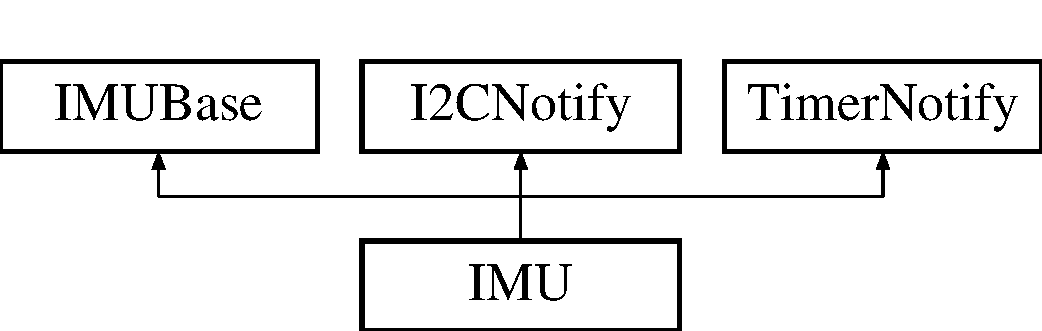
\includegraphics[height=2.000000cm]{class_i_m_u}
\end{center}
\end{figure}
\subsection*{Classes}
\begin{DoxyCompactItemize}
\item 
struct \hyperlink{struct_i_m_u_1_1reg_write}{regWrite}
\end{DoxyCompactItemize}
\subsection*{Public Member Functions}
\begin{DoxyCompactItemize}
\item 
\hyperlink{class_i_m_u_aa628daa06d0e29e4aa84bb8336649134}{IMU} (I2C\_\-Master $\ast$pMas, uint8\_\-t gID, uint8\_\-t aID)
\begin{DoxyCompactList}\small\item\em Constructor for a single \hyperlink{class_i_m_u}{IMU} I2C Channel. \item\end{DoxyCompactList}\item 
\hyperlink{class_i_m_u_ac3b25bbd72ae020b61012fd4ebf8a188}{IMU} (I2C\_\-Master $\ast$pMas, uint8\_\-t gID, uint8\_\-t aID, uint8\_\-t gID2, uint8\_\-t aID2)
\begin{DoxyCompactList}\small\item\em Constructor for a double \hyperlink{class_i_m_u}{IMU} I2C Channel. \item\end{DoxyCompactList}\item 
void \hyperlink{class_i_m_u_afedf46bdad68cb4002af8bf46530d265}{SetDebugPort} (DebugPort $\ast$pPort)
\item 
void \hyperlink{class_i_m_u_a6f86c79e66c4262093c2d65fe3fee45c}{SetDebugPort2} (DebugPort $\ast$pPort)
\item 
virtual void \hyperlink{class_i_m_u_a13191357ff93d02f6cc7aa7e55b13d67}{Reset} ()
\item 
virtual void \hyperlink{class_i_m_u_a7705d9d642b093a670e78534c9b2d3db}{SampleRate} (uint16\_\-t)
\item 
virtual int \hyperlink{class_i_m_u_a290737d42de965c15c8327edfc516ffd}{Setup} ()
\item 
virtual int \hyperlink{class_i_m_u_a7c03f7a423240538756a62441b298d01}{Start} ()
\item 
virtual int \hyperlink{class_i_m_u_af0841bed4167f7a4eb12c40d7b8e615e}{Stop} ()
\item 
virtual int \hyperlink{class_i_m_u_a004d2bb9e6155f45edc9e46bce730644}{ForceStartStop} ()
\item 
virtual bool \hyperlink{class_i_m_u_ade0f7e6be2eda441bfaa2cb372fec55a}{Busy} ()
\item 
virtual void \hyperlink{class_i_m_u_a187dc9de30f97f5154e0ff904eb6ee1a}{ResetTimer} ()
\item 
virtual void \hyperlink{class_i_m_u_a86f05be645d2096f0b2b3cfbe8ea0ce8}{UseGyro} (bool bEnable)
\item 
virtual bool \hyperlink{class_i_m_u_a078d2f3ad27475c9afcaf09c44886e4c}{DataReady} ()
\item 
virtual uint8\_\-t $\ast$ \hyperlink{class_i_m_u_a4f72b7f99fc42f30c9478ba7ed65654e}{GetPacketData} (uint8\_\-t $\ast$)
\item 
virtual void \hyperlink{class_i_m_u_a74feb2946c48a92b251e28ac256d887b}{CheckIDs} (\hyperlink{class_hardware_serial}{HardwareSerial} $\ast$pSerial)
\item 
virtual void \hyperlink{class_i_m_u_a98f9a8244dd1a07f8771450097371b2c}{ResetDevices} ()
\item 
void \hyperlink{class_i_m_u_a66680475b844fbf334a0e4e7c5fe845b}{SetTimer} (\hyperlink{class_timer_cntr}{TimerCntr} $\ast$pTimer)
\item 
void \hyperlink{class_i_m_u_a3ce9934e64dff87e18b6cc3f3700f72f}{SetTimerPeriod} ()
\item 
virtual void \hyperlink{class_i_m_u_a71568969beb6ee7d4b596f8c0a91faf9}{I2CWriteDone} ()
\item 
virtual void \hyperlink{class_i_m_u_ab4124ae29a64365787c2c03b3ab09c6c}{I2CReadDone} ()
\item 
virtual void \hyperlink{class_i_m_u_aad041ec91d266e9fc15d22de17ffccad}{I2CBusError} ()
\item 
virtual void \hyperlink{class_i_m_u_a7d4a2a761fb4956ebd9ce0b0cda69556}{I2CArbLost} ()
\item 
virtual void \hyperlink{class_i_m_u_a161f80bfcb7195196754a18eddedaf12}{I2CNack} ()
\item 
void \hyperlink{class_i_m_u_acf8e9ee1971e527c255c046d3d3c1fe9}{FailRecovery} ()
\end{DoxyCompactItemize}
\begin{Indent}{\bf Interrupt Handlers}\par
{\em These handlers receive interupts from the Timer class. We registered to received these calls with the Notify function. In some cases we might have 2 or more objects that will send us interrupt notifications, in this case we give each object an ID that is passed back so that we know which one caused the interrupt.

For the IMUManager, there is only a single Timer, so the ID is always 0. }\begin{DoxyCompactItemize}
\item 
virtual void \hyperlink{class_i_m_u_ae56d268445b752f9720c814cb294ba40}{err} (uint8\_\-t id)
\begin{DoxyCompactList}\small\item\em Timer Error -\/ ignored. \item\end{DoxyCompactList}\item 
virtual void \hyperlink{class_i_m_u_aefbd4e2f7f3928cf44c00a96d61c3546}{ovf} (uint8\_\-t id)
\item 
virtual void \hyperlink{class_i_m_u_ad2215ab5585c1f9512b91ef309dabf88}{ccx} (uint8\_\-t id, uint8\_\-t idx)
\begin{DoxyCompactList}\small\item\em Timer Capture Compare -\/ not used. \item\end{DoxyCompactList}\end{DoxyCompactItemize}
\end{Indent}
\subsection*{Protected Member Functions}
\begin{DoxyCompactItemize}
\item 
void \hyperlink{class_i_m_u_aadf38b912ad23374c4ee8e40fb9f3638}{Run} ()
\item 
int \hyperlink{class_i_m_u_a8dfecb837ea9fcf9d190423dca9beb7f}{StartTransaction} ()
\item 
void \hyperlink{class_i_m_u_ac39f14c617d4eea9de6175497744465a}{ProcessTransaction} ()
\item 
int \hyperlink{class_i_m_u_af4bede5261a1d6018c72782d8c54445e}{Configure} (uint8\_\-t idx)
\item 
int \hyperlink{class_i_m_u_af80eef2eb22d08faf697dd708b18303c}{Wr} (uint8\_\-t ID, uint8\_\-t addr, uint8\_\-t data)
\item 
int \hyperlink{class_i_m_u_ab6c8ef618465524c88a021e2206b2de5}{Rd} (uint8\_\-t ID, uint8\_\-t addr, uint8\_\-t cnt, uint8\_\-t $\ast$pData)
\item 
int \hyperlink{class_i_m_u_a2c38589ebcb357dfc8f987a5d41c845b}{WrAsync} (uint8\_\-t ID, uint8\_\-t addr, uint8\_\-t data)
\item 
int \hyperlink{class_i_m_u_ad39e85995898b9251032c89a3587974c}{RdAsync} (uint8\_\-t ID, uint8\_\-t addr, uint8\_\-t cnt)
\item 
void \hyperlink{class_i_m_u_a07362afd858bca1ce960f3809248e4e9}{ReadWord} (uint16\_\-t $\ast$pData)
\item 
void \hyperlink{class_i_m_u_a5b58d543be70886335e439a2b4f28a8e}{StoreGyroData} (uint8\_\-t idx)
\item 
void \hyperlink{class_i_m_u_ae9c290e496eb2a76aefc626c81fe4da9}{StoreAccData} (uint8\_\-t idx)
\item 
void \hyperlink{class_i_m_u_a14f3437170b38602f281b3f97d9ce129}{PushData} (uint8\_\-t idx)
\begin{DoxyCompactList}\small\item\em Push the data in the temporary buffer onto the appropriate fifo. \item\end{DoxyCompactList}\item 
void \hyperlink{class_i_m_u_a5d80a28d98df12c536f525b56b7e5abe}{SetState} (\hyperlink{class_i_m_u_a7b5e1bf1cf1407b3e4cf0dd2e18b523f}{StateType} s)
\item 
void \hyperlink{class_i_m_u_a7f9a7744a4fa3ea40da008cabd5da7b7}{MarkPos} (\hyperlink{class_i_m_u_ad01128d82debc1e4213affe4858f3144}{PosType} p)
\item 
bool \hyperlink{class_i_m_u_a0bd84946a218d910f248cfa8edf00a5c}{DataAvail} ()
\item 
bool \hyperlink{class_i_m_u_a492e190eef142fc6bc674cca4700f1e3}{DataAvail} (uint8\_\-t idx)
\item 
void \hyperlink{class_i_m_u_ab3992da77876e9b5cae8bc9d1334ff7b}{ResetBusyTime} ()
\item 
bool \hyperlink{class_i_m_u_a6a61733d65cf2b60db212e0be9a00fed}{BusyTimeout} ()
\item 
void \hyperlink{class_i_m_u_a89de27b845ce9e103436cfb7ae8e6441}{ResetFailStats} ()
\end{DoxyCompactItemize}
\subsection*{Private Types}
\begin{DoxyCompactItemize}
\item 
enum \hyperlink{class_i_m_u_a7b5e1bf1cf1407b3e4cf0dd2e18b523f}{StateType} \{ \par
\hyperlink{class_i_m_u_a7b5e1bf1cf1407b3e4cf0dd2e18b523fa82181a217d68f26cba06b38cfb94c1bc}{sIdle} =  0, 
\hyperlink{class_i_m_u_a7b5e1bf1cf1407b3e4cf0dd2e18b523fae3a15f0845da0f426c48b6bd9ed01b21}{sConfigure} =  1, 
\hyperlink{class_i_m_u_a7b5e1bf1cf1407b3e4cf0dd2e18b523fa98a87654cac5bbc7d12c9701563dbae5}{sConfigured} =  2, 
\hyperlink{class_i_m_u_a7b5e1bf1cf1407b3e4cf0dd2e18b523fa4d7c7afff1b740c59d740b9b77a8d18c}{sWait} =  5, 
\par
\hyperlink{class_i_m_u_a7b5e1bf1cf1407b3e4cf0dd2e18b523fa8f3b3efb815c4ee9396ccb1fda939f77}{sReadGyro1} =  8, 
\hyperlink{class_i_m_u_a7b5e1bf1cf1407b3e4cf0dd2e18b523fa7e6ba39651fb8aca4abcdf80ed789d8b}{sReadAcc1} =  9, 
\hyperlink{class_i_m_u_a7b5e1bf1cf1407b3e4cf0dd2e18b523fa2e538ebe471a9482d15ab162ec3bdc6d}{sReadGyro2} =  10, 
\hyperlink{class_i_m_u_a7b5e1bf1cf1407b3e4cf0dd2e18b523fa4d82e2432f2e2075cef6143740c4df59}{sReadAcc2} =  11, 
\par
\hyperlink{class_i_m_u_a7b5e1bf1cf1407b3e4cf0dd2e18b523fae27080f67607320b8cc57d8402a07277}{sErrRecover} =  12
 \}
\item 
enum \hyperlink{class_i_m_u_ad01128d82debc1e4213affe4858f3144}{PosType} \{ \par
\hyperlink{class_i_m_u_ad01128d82debc1e4213affe4858f3144a1d2d6c166c92bec6d19b37a6dbeeaf8c}{pStart} =  0, 
\hyperlink{class_i_m_u_ad01128d82debc1e4213affe4858f3144a9cb1b471b394a5a3a87c6bab61ae00e4}{pRun} =  1, 
\hyperlink{class_i_m_u_ad01128d82debc1e4213affe4858f3144ac2332a4383aa00818b3fc4ed83ec1f4d}{pWriteDn} =  2, 
\hyperlink{class_i_m_u_ad01128d82debc1e4213affe4858f3144a1b257baca1eb9eb3e7192a01770cce76}{pReadDn} =  3, 
\par
\hyperlink{class_i_m_u_ad01128d82debc1e4213affe4858f3144ac361e1f3b3b93592825ae06da0309c62}{pNack} =  4, 
\hyperlink{class_i_m_u_ad01128d82debc1e4213affe4858f3144a3db70da4b0066e7738bed5e25f4fc405}{pBusErr} =  5, 
\hyperlink{class_i_m_u_ad01128d82debc1e4213affe4858f3144a5b061676aa01e1049ff07e5a191c9af8}{pArbLost} =  6, 
\hyperlink{class_i_m_u_ad01128d82debc1e4213affe4858f3144a73419f05716e41c972241a4fc0c6ead0}{pSetup} =  7
 \}
\item 
enum \hyperlink{class_i_m_u_a4edeb07a848734657792b4ef8749fb97}{FailType} \{ \hyperlink{class_i_m_u_a4edeb07a848734657792b4ef8749fb97ac049bda2fb043b649de1cdb8d203aac2}{fNone} =  0, 
\hyperlink{class_i_m_u_a4edeb07a848734657792b4ef8749fb97a17dff6c1392332855f9e83033dff49f8}{fNack} =  1, 
\hyperlink{class_i_m_u_a4edeb07a848734657792b4ef8749fb97a4f33b2c6a17b90c350b4ad6f5f71cc34}{fBusErr} =  2, 
\hyperlink{class_i_m_u_a4edeb07a848734657792b4ef8749fb97acf94640c5a7cfb3a4fc806dabf005260}{fArbLost} =  3
 \}
\item 
enum \hyperlink{class_i_m_u_a5a642d4cba90a478ae8c3312a47a57ce}{ProcessType} \{ \hyperlink{class_i_m_u_a5a642d4cba90a478ae8c3312a47a57cea978a6a5569595a7e86fe7e48d2684a7f}{ptTimer}, 
\hyperlink{class_i_m_u_a5a642d4cba90a478ae8c3312a47a57cea32f99524523d0d11cbd3348ee2fba9ea}{ptI2CWrite}, 
\hyperlink{class_i_m_u_a5a642d4cba90a478ae8c3312a47a57cea5aabc602033dc4f845e45d33fe939688}{ptI2CRead}, 
\hyperlink{class_i_m_u_a5a642d4cba90a478ae8c3312a47a57ceab11e066033d0049893742894a7252fc8}{ptI2CNack}
 \}
\item 
typedef enum \hyperlink{class_i_m_u_a7b5e1bf1cf1407b3e4cf0dd2e18b523f}{IMU::StateType} \hyperlink{class_i_m_u_a2c1f560a0bc80d0bd06bb56a614aeedd}{StateType}
\item 
typedef enum \hyperlink{class_i_m_u_ad01128d82debc1e4213affe4858f3144}{IMU::PosType} \hyperlink{class_i_m_u_ad82ee88c050235081f004f81a5724e09}{PosType}
\item 
typedef enum \hyperlink{class_i_m_u_a4edeb07a848734657792b4ef8749fb97}{IMU::FailType} \hyperlink{class_i_m_u_a4baf4d6e504dcb71c4afab34be225620}{FailType}
\item 
typedef struct \hyperlink{struct_i_m_u_1_1reg_write}{IMU::regWrite} \hyperlink{class_i_m_u_a1960eeaec92b6b60d4f6c9e28b042b80}{RegWriteType}
\end{DoxyCompactItemize}
\subsection*{Private Attributes}
\begin{DoxyCompactItemize}
\item 
\hyperlink{class_i_m_u_a7b5e1bf1cf1407b3e4cf0dd2e18b523f}{StateType} \hyperlink{class_i_m_u_a2e3c70d02cc2b3dd98ce8153d02cf04e}{\_\-State}
\item 
\hyperlink{class_i_m_u_a7b5e1bf1cf1407b3e4cf0dd2e18b523f}{StateType} \hyperlink{class_i_m_u_aca284ca1bcf10458005d4ca630833ea9}{\_\-previousState}
\item 
\hyperlink{class_i_m_u_a4edeb07a848734657792b4ef8749fb97}{FailType} \hyperlink{class_i_m_u_a39ed63b67b50c67520c5f8e5a2c26b26}{\_\-failType}
\item 
I2C\_\-Master $\ast$ \hyperlink{class_i_m_u_a466148932203b7250c83a4c5bb684ca1}{\_\-pMas}
\item 
bool \hyperlink{class_i_m_u_a62978e791838c3b4829e1d3d683e99b2}{\_\-bDualChan}
\item 
uint8\_\-t \hyperlink{class_i_m_u_a27df580b4559aaf3234469bfe16eb158}{\_\-numChans}
\item 
uint8\_\-t \hyperlink{class_i_m_u_a08a36cacd3d4d14b4aa834a657422b15}{\_\-currChannel}
\item 
uint16\_\-t \hyperlink{class_i_m_u_aa9a352174cae0cd174cb91ef09a47fe4}{\_\-currFifoReadLen} \mbox{[}2\mbox{]}
\item 
bool \hyperlink{class_i_m_u_a53aa928d2d68a5287da893bd157e7cbe}{\_\-configOkay} \mbox{[}2\mbox{]}
\item 
uint8\_\-t \hyperlink{class_i_m_u_a47ffe20a032e3a890cd3891793a60a40}{\_\-gID} \mbox{[}2\mbox{]}
\item 
uint8\_\-t \hyperlink{class_i_m_u_a10141bdc27465c95de6c8285d1542d78}{\_\-aID} \mbox{[}2\mbox{]}
\item 
uint8\_\-t \hyperlink{class_i_m_u_a3f9e6159234449cde8f5e72da8acf751}{\_\-DLPF}
\item 
uint8\_\-t \hyperlink{class_i_m_u_a059c02011a10bb90aecc9692ed345771}{\_\-FullScale}
\item 
uint8\_\-t \hyperlink{class_i_m_u_a4dbeaf17fd1ae9b41b5c3fe61706e5f1}{\_\-ClkSel}
\item 
uint16\_\-t \hyperlink{class_i_m_u_aafe9be107385c7ccedeb1539cf6d7fce}{\_\-Rate}
\item 
IMUPacketFifo \hyperlink{class_i_m_u_a43cbdffbfb85749212ede7f78ab6f1e0}{\_\-rdFifo}
\item 
IMUPacketFifo \hyperlink{class_i_m_u_a8eb715f35f45943bedc2b9280c3f2cd3}{\_\-rdFifo2}
\item 
bool \hyperlink{class_i_m_u_a0cee90ebd5d0b57fa5ad3890c65108e2}{\_\-bUseGyro}
\item 
uint8\_\-t \hyperlink{class_i_m_u_ab87a54288295d4d10d605cf6c21d4d0f}{\_\-dataBuffer} \mbox{[}2\mbox{]}\mbox{[}20\mbox{]}
\begin{DoxyCompactList}\small\item\em This buffer is used to store data until we push it into the fifo. \item\end{DoxyCompactList}\item 
bool \hyperlink{class_i_m_u_a8a71f0728b2d849d1d8e54fcb58aad4e}{\_\-bDataReady} \mbox{[}2\mbox{]}
\item 
uint16\_\-t \hyperlink{class_i_m_u_a9f7f36da069258a5615886e098527100}{\_\-fifoLen} \mbox{[}2\mbox{]}
\item 
\hyperlink{class_timer_cntr}{TimerCntr} $\ast$ \hyperlink{class_i_m_u_a16e73b1457a346aed16d4b61fae7f2c4}{\_\-pTimer}
\item 
bool \hyperlink{class_i_m_u_a547fe1fb8adb34917aa08663919b97df}{\_\-bRun}
\item 
uint16\_\-t \hyperlink{class_i_m_u_a1e646aa38b84721fc650ef5d3388cc14}{\_\-failCount}
\item 
uint8\_\-t \hyperlink{class_i_m_u_a30c8553ab21b5d6e618c2616f25dafb1}{\_\-nackCount}
\begin{DoxyCompactList}\small\item\em used for recover logic \item\end{DoxyCompactList}\item 
bool \hyperlink{class_i_m_u_a12238a84e20f54c5fe799e0b37feb0ea}{\_\-bFailDetected}
\item 
unsigned int \hyperlink{class_i_m_u_adce31ce2a3317918d73b47e94a2d9227}{\_\-busyWaitTime}
\item 
DebugPort $\ast$ \hyperlink{class_i_m_u_a83a2ffaf84cc04f17ff0301181c45366}{\_\-pDBGPort}
\item 
DebugPort $\ast$ \hyperlink{class_i_m_u_a1cf5672a28049d5885a2958010188928}{\_\-pDBGPort2}
\end{DoxyCompactItemize}


\subsection{Detailed Description}


Definition at line 38 of file IMU.h.



\subsection{Member Typedef Documentation}
\hypertarget{class_i_m_u_a4baf4d6e504dcb71c4afab34be225620}{
\index{IMU@{IMU}!FailType@{FailType}}
\index{FailType@{FailType}!IMU@{IMU}}
\subsubsection[{FailType}]{\setlength{\rightskip}{0pt plus 5cm}typedef enum {\bf IMU::FailType}  {\bf IMU::FailType}\hspace{0.3cm}{\ttfamily  \mbox{[}private\mbox{]}}}}
\label{class_i_m_u_a4baf4d6e504dcb71c4afab34be225620}
\hypertarget{class_i_m_u_ad82ee88c050235081f004f81a5724e09}{
\index{IMU@{IMU}!PosType@{PosType}}
\index{PosType@{PosType}!IMU@{IMU}}
\subsubsection[{PosType}]{\setlength{\rightskip}{0pt plus 5cm}typedef enum {\bf IMU::PosType}  {\bf IMU::PosType}\hspace{0.3cm}{\ttfamily  \mbox{[}private\mbox{]}}}}
\label{class_i_m_u_ad82ee88c050235081f004f81a5724e09}
\hypertarget{class_i_m_u_a1960eeaec92b6b60d4f6c9e28b042b80}{
\index{IMU@{IMU}!RegWriteType@{RegWriteType}}
\index{RegWriteType@{RegWriteType}!IMU@{IMU}}
\subsubsection[{RegWriteType}]{\setlength{\rightskip}{0pt plus 5cm}typedef struct {\bf IMU::regWrite}  {\bf IMU::RegWriteType}\hspace{0.3cm}{\ttfamily  \mbox{[}private\mbox{]}}}}
\label{class_i_m_u_a1960eeaec92b6b60d4f6c9e28b042b80}
\hypertarget{class_i_m_u_a2c1f560a0bc80d0bd06bb56a614aeedd}{
\index{IMU@{IMU}!StateType@{StateType}}
\index{StateType@{StateType}!IMU@{IMU}}
\subsubsection[{StateType}]{\setlength{\rightskip}{0pt plus 5cm}typedef enum {\bf IMU::StateType}  {\bf IMU::StateType}\hspace{0.3cm}{\ttfamily  \mbox{[}private\mbox{]}}}}
\label{class_i_m_u_a2c1f560a0bc80d0bd06bb56a614aeedd}


\subsection{Member Enumeration Documentation}
\hypertarget{class_i_m_u_a4edeb07a848734657792b4ef8749fb97}{
\index{IMU@{IMU}!FailType@{FailType}}
\index{FailType@{FailType}!IMU@{IMU}}
\subsubsection[{FailType}]{\setlength{\rightskip}{0pt plus 5cm}enum {\bf IMU::FailType}\hspace{0.3cm}{\ttfamily  \mbox{[}private\mbox{]}}}}
\label{class_i_m_u_a4edeb07a848734657792b4ef8749fb97}
\begin{Desc}
\item[Enumerator: ]\par
\begin{description}
\index{fNone@{fNone}!IMU@{IMU}}\index{IMU@{IMU}!fNone@{fNone}}\item[{\em 
\hypertarget{class_i_m_u_a4edeb07a848734657792b4ef8749fb97ac049bda2fb043b649de1cdb8d203aac2}{
fNone}
\label{class_i_m_u_a4edeb07a848734657792b4ef8749fb97ac049bda2fb043b649de1cdb8d203aac2}
}]\index{fNack@{fNack}!IMU@{IMU}}\index{IMU@{IMU}!fNack@{fNack}}\item[{\em 
\hypertarget{class_i_m_u_a4edeb07a848734657792b4ef8749fb97a17dff6c1392332855f9e83033dff49f8}{
fNack}
\label{class_i_m_u_a4edeb07a848734657792b4ef8749fb97a17dff6c1392332855f9e83033dff49f8}
}]\index{fBusErr@{fBusErr}!IMU@{IMU}}\index{IMU@{IMU}!fBusErr@{fBusErr}}\item[{\em 
\hypertarget{class_i_m_u_a4edeb07a848734657792b4ef8749fb97a4f33b2c6a17b90c350b4ad6f5f71cc34}{
fBusErr}
\label{class_i_m_u_a4edeb07a848734657792b4ef8749fb97a4f33b2c6a17b90c350b4ad6f5f71cc34}
}]\index{fArbLost@{fArbLost}!IMU@{IMU}}\index{IMU@{IMU}!fArbLost@{fArbLost}}\item[{\em 
\hypertarget{class_i_m_u_a4edeb07a848734657792b4ef8749fb97acf94640c5a7cfb3a4fc806dabf005260}{
fArbLost}
\label{class_i_m_u_a4edeb07a848734657792b4ef8749fb97acf94640c5a7cfb3a4fc806dabf005260}
}]\end{description}
\end{Desc}



Definition at line 67 of file IMU.h.


\begin{DoxyCode}
                          {
        fNone           = 0,
        fNack           = 1,
        fBusErr         = 2,
        fArbLost        = 3
    } FailType;
\end{DoxyCode}
\hypertarget{class_i_m_u_ad01128d82debc1e4213affe4858f3144}{
\index{IMU@{IMU}!PosType@{PosType}}
\index{PosType@{PosType}!IMU@{IMU}}
\subsubsection[{PosType}]{\setlength{\rightskip}{0pt plus 5cm}enum {\bf IMU::PosType}\hspace{0.3cm}{\ttfamily  \mbox{[}private\mbox{]}}}}
\label{class_i_m_u_ad01128d82debc1e4213affe4858f3144}
\begin{Desc}
\item[Enumerator: ]\par
\begin{description}
\index{pStart@{pStart}!IMU@{IMU}}\index{IMU@{IMU}!pStart@{pStart}}\item[{\em 
\hypertarget{class_i_m_u_ad01128d82debc1e4213affe4858f3144a1d2d6c166c92bec6d19b37a6dbeeaf8c}{
pStart}
\label{class_i_m_u_ad01128d82debc1e4213affe4858f3144a1d2d6c166c92bec6d19b37a6dbeeaf8c}
}]\index{pRun@{pRun}!IMU@{IMU}}\index{IMU@{IMU}!pRun@{pRun}}\item[{\em 
\hypertarget{class_i_m_u_ad01128d82debc1e4213affe4858f3144a9cb1b471b394a5a3a87c6bab61ae00e4}{
pRun}
\label{class_i_m_u_ad01128d82debc1e4213affe4858f3144a9cb1b471b394a5a3a87c6bab61ae00e4}
}]\index{pWriteDn@{pWriteDn}!IMU@{IMU}}\index{IMU@{IMU}!pWriteDn@{pWriteDn}}\item[{\em 
\hypertarget{class_i_m_u_ad01128d82debc1e4213affe4858f3144ac2332a4383aa00818b3fc4ed83ec1f4d}{
pWriteDn}
\label{class_i_m_u_ad01128d82debc1e4213affe4858f3144ac2332a4383aa00818b3fc4ed83ec1f4d}
}]\index{pReadDn@{pReadDn}!IMU@{IMU}}\index{IMU@{IMU}!pReadDn@{pReadDn}}\item[{\em 
\hypertarget{class_i_m_u_ad01128d82debc1e4213affe4858f3144a1b257baca1eb9eb3e7192a01770cce76}{
pReadDn}
\label{class_i_m_u_ad01128d82debc1e4213affe4858f3144a1b257baca1eb9eb3e7192a01770cce76}
}]\index{pNack@{pNack}!IMU@{IMU}}\index{IMU@{IMU}!pNack@{pNack}}\item[{\em 
\hypertarget{class_i_m_u_ad01128d82debc1e4213affe4858f3144ac361e1f3b3b93592825ae06da0309c62}{
pNack}
\label{class_i_m_u_ad01128d82debc1e4213affe4858f3144ac361e1f3b3b93592825ae06da0309c62}
}]\index{pBusErr@{pBusErr}!IMU@{IMU}}\index{IMU@{IMU}!pBusErr@{pBusErr}}\item[{\em 
\hypertarget{class_i_m_u_ad01128d82debc1e4213affe4858f3144a3db70da4b0066e7738bed5e25f4fc405}{
pBusErr}
\label{class_i_m_u_ad01128d82debc1e4213affe4858f3144a3db70da4b0066e7738bed5e25f4fc405}
}]\index{pArbLost@{pArbLost}!IMU@{IMU}}\index{IMU@{IMU}!pArbLost@{pArbLost}}\item[{\em 
\hypertarget{class_i_m_u_ad01128d82debc1e4213affe4858f3144a5b061676aa01e1049ff07e5a191c9af8}{
pArbLost}
\label{class_i_m_u_ad01128d82debc1e4213affe4858f3144a5b061676aa01e1049ff07e5a191c9af8}
}]\index{pSetup@{pSetup}!IMU@{IMU}}\index{IMU@{IMU}!pSetup@{pSetup}}\item[{\em 
\hypertarget{class_i_m_u_ad01128d82debc1e4213affe4858f3144a73419f05716e41c972241a4fc0c6ead0}{
pSetup}
\label{class_i_m_u_ad01128d82debc1e4213affe4858f3144a73419f05716e41c972241a4fc0c6ead0}
}]\end{description}
\end{Desc}



Definition at line 56 of file IMU.h.


\begin{DoxyCode}
                         {
        pStart          = 0,
        pRun            = 1,
        pWriteDn        = 2,
        pReadDn         = 3,
        pNack           = 4,
        pBusErr         = 5,
        pArbLost        = 6,
        pSetup          = 7
    } PosType;
\end{DoxyCode}
\hypertarget{class_i_m_u_a5a642d4cba90a478ae8c3312a47a57ce}{
\index{IMU@{IMU}!ProcessType@{ProcessType}}
\index{ProcessType@{ProcessType}!IMU@{IMU}}
\subsubsection[{ProcessType}]{\setlength{\rightskip}{0pt plus 5cm}enum {\bf IMU::ProcessType}\hspace{0.3cm}{\ttfamily  \mbox{[}private\mbox{]}}}}
\label{class_i_m_u_a5a642d4cba90a478ae8c3312a47a57ce}
\begin{Desc}
\item[Enumerator: ]\par
\begin{description}
\index{ptTimer@{ptTimer}!IMU@{IMU}}\index{IMU@{IMU}!ptTimer@{ptTimer}}\item[{\em 
\hypertarget{class_i_m_u_a5a642d4cba90a478ae8c3312a47a57cea978a6a5569595a7e86fe7e48d2684a7f}{
ptTimer}
\label{class_i_m_u_a5a642d4cba90a478ae8c3312a47a57cea978a6a5569595a7e86fe7e48d2684a7f}
}]\index{ptI2CWrite@{ptI2CWrite}!IMU@{IMU}}\index{IMU@{IMU}!ptI2CWrite@{ptI2CWrite}}\item[{\em 
\hypertarget{class_i_m_u_a5a642d4cba90a478ae8c3312a47a57cea32f99524523d0d11cbd3348ee2fba9ea}{
ptI2CWrite}
\label{class_i_m_u_a5a642d4cba90a478ae8c3312a47a57cea32f99524523d0d11cbd3348ee2fba9ea}
}]\index{ptI2CRead@{ptI2CRead}!IMU@{IMU}}\index{IMU@{IMU}!ptI2CRead@{ptI2CRead}}\item[{\em 
\hypertarget{class_i_m_u_a5a642d4cba90a478ae8c3312a47a57cea5aabc602033dc4f845e45d33fe939688}{
ptI2CRead}
\label{class_i_m_u_a5a642d4cba90a478ae8c3312a47a57cea5aabc602033dc4f845e45d33fe939688}
}]\index{ptI2CNack@{ptI2CNack}!IMU@{IMU}}\index{IMU@{IMU}!ptI2CNack@{ptI2CNack}}\item[{\em 
\hypertarget{class_i_m_u_a5a642d4cba90a478ae8c3312a47a57ceab11e066033d0049893742894a7252fc8}{
ptI2CNack}
\label{class_i_m_u_a5a642d4cba90a478ae8c3312a47a57ceab11e066033d0049893742894a7252fc8}
}]\end{description}
\end{Desc}



Definition at line 80 of file IMU.h.


\begin{DoxyCode}
                  {
        ptTimer,
        ptI2CWrite,
        ptI2CRead,
        ptI2CNack
    } ProcessType;
\end{DoxyCode}
\hypertarget{class_i_m_u_a7b5e1bf1cf1407b3e4cf0dd2e18b523f}{
\index{IMU@{IMU}!StateType@{StateType}}
\index{StateType@{StateType}!IMU@{IMU}}
\subsubsection[{StateType}]{\setlength{\rightskip}{0pt plus 5cm}enum {\bf IMU::StateType}\hspace{0.3cm}{\ttfamily  \mbox{[}private\mbox{]}}}}
\label{class_i_m_u_a7b5e1bf1cf1407b3e4cf0dd2e18b523f}
\begin{Desc}
\item[Enumerator: ]\par
\begin{description}
\index{sIdle@{sIdle}!IMU@{IMU}}\index{IMU@{IMU}!sIdle@{sIdle}}\item[{\em 
\hypertarget{class_i_m_u_a7b5e1bf1cf1407b3e4cf0dd2e18b523fa82181a217d68f26cba06b38cfb94c1bc}{
sIdle}
\label{class_i_m_u_a7b5e1bf1cf1407b3e4cf0dd2e18b523fa82181a217d68f26cba06b38cfb94c1bc}
}]\index{sConfigure@{sConfigure}!IMU@{IMU}}\index{IMU@{IMU}!sConfigure@{sConfigure}}\item[{\em 
\hypertarget{class_i_m_u_a7b5e1bf1cf1407b3e4cf0dd2e18b523fae3a15f0845da0f426c48b6bd9ed01b21}{
sConfigure}
\label{class_i_m_u_a7b5e1bf1cf1407b3e4cf0dd2e18b523fae3a15f0845da0f426c48b6bd9ed01b21}
}]\index{sConfigured@{sConfigured}!IMU@{IMU}}\index{IMU@{IMU}!sConfigured@{sConfigured}}\item[{\em 
\hypertarget{class_i_m_u_a7b5e1bf1cf1407b3e4cf0dd2e18b523fa98a87654cac5bbc7d12c9701563dbae5}{
sConfigured}
\label{class_i_m_u_a7b5e1bf1cf1407b3e4cf0dd2e18b523fa98a87654cac5bbc7d12c9701563dbae5}
}]\index{sWait@{sWait}!IMU@{IMU}}\index{IMU@{IMU}!sWait@{sWait}}\item[{\em 
\hypertarget{class_i_m_u_a7b5e1bf1cf1407b3e4cf0dd2e18b523fa4d7c7afff1b740c59d740b9b77a8d18c}{
sWait}
\label{class_i_m_u_a7b5e1bf1cf1407b3e4cf0dd2e18b523fa4d7c7afff1b740c59d740b9b77a8d18c}
}]\index{sReadGyro1@{sReadGyro1}!IMU@{IMU}}\index{IMU@{IMU}!sReadGyro1@{sReadGyro1}}\item[{\em 
\hypertarget{class_i_m_u_a7b5e1bf1cf1407b3e4cf0dd2e18b523fa8f3b3efb815c4ee9396ccb1fda939f77}{
sReadGyro1}
\label{class_i_m_u_a7b5e1bf1cf1407b3e4cf0dd2e18b523fa8f3b3efb815c4ee9396ccb1fda939f77}
}]\index{sReadAcc1@{sReadAcc1}!IMU@{IMU}}\index{IMU@{IMU}!sReadAcc1@{sReadAcc1}}\item[{\em 
\hypertarget{class_i_m_u_a7b5e1bf1cf1407b3e4cf0dd2e18b523fa7e6ba39651fb8aca4abcdf80ed789d8b}{
sReadAcc1}
\label{class_i_m_u_a7b5e1bf1cf1407b3e4cf0dd2e18b523fa7e6ba39651fb8aca4abcdf80ed789d8b}
}]\index{sReadGyro2@{sReadGyro2}!IMU@{IMU}}\index{IMU@{IMU}!sReadGyro2@{sReadGyro2}}\item[{\em 
\hypertarget{class_i_m_u_a7b5e1bf1cf1407b3e4cf0dd2e18b523fa2e538ebe471a9482d15ab162ec3bdc6d}{
sReadGyro2}
\label{class_i_m_u_a7b5e1bf1cf1407b3e4cf0dd2e18b523fa2e538ebe471a9482d15ab162ec3bdc6d}
}]\index{sReadAcc2@{sReadAcc2}!IMU@{IMU}}\index{IMU@{IMU}!sReadAcc2@{sReadAcc2}}\item[{\em 
\hypertarget{class_i_m_u_a7b5e1bf1cf1407b3e4cf0dd2e18b523fa4d82e2432f2e2075cef6143740c4df59}{
sReadAcc2}
\label{class_i_m_u_a7b5e1bf1cf1407b3e4cf0dd2e18b523fa4d82e2432f2e2075cef6143740c4df59}
}]\index{sErrRecover@{sErrRecover}!IMU@{IMU}}\index{IMU@{IMU}!sErrRecover@{sErrRecover}}\item[{\em 
\hypertarget{class_i_m_u_a7b5e1bf1cf1407b3e4cf0dd2e18b523fae27080f67607320b8cc57d8402a07277}{
sErrRecover}
\label{class_i_m_u_a7b5e1bf1cf1407b3e4cf0dd2e18b523fae27080f67607320b8cc57d8402a07277}
}]\end{description}
\end{Desc}



Definition at line 40 of file IMU.h.


\begin{DoxyCode}
                           {
        sIdle           = 0,
        sConfigure      = 1,
        sConfigured     = 2,
//        sFifoInit1      = 3,
//        sFifoInit2      = 4,
        sWait           = 5,       
//        sReadLen1       = 6,
//        sReadLen2       = 7,
        sReadGyro1      = 8,
        sReadAcc1       = 9,
        sReadGyro2      = 10,
        sReadAcc2       = 11,
        sErrRecover     = 12
    } StateType;
\end{DoxyCode}


\subsection{Constructor \& Destructor Documentation}
\hypertarget{class_i_m_u_aa628daa06d0e29e4aa84bb8336649134}{
\index{IMU@{IMU}!IMU@{IMU}}
\index{IMU@{IMU}!IMU@{IMU}}
\subsubsection[{IMU}]{\setlength{\rightskip}{0pt plus 5cm}IMU::IMU (
\begin{DoxyParamCaption}
\item[{I2C\_\-Master $\ast$}]{pMas, }
\item[{uint8\_\-t}]{gID, }
\item[{uint8\_\-t}]{aID}
\end{DoxyParamCaption}
)}}
\label{class_i_m_u_aa628daa06d0e29e4aa84bb8336649134}


Constructor for a single \hyperlink{class_i_m_u}{IMU} I2C Channel. 



Definition at line 19 of file IMU.cpp.



References \_\-aID, \_\-bDualChan, \_\-bRun, \_\-bUseGyro, \_\-ClkSel, \_\-DLPF, \_\-FullScale, \_\-gID, \_\-numChans, \_\-pDBGPort, \_\-pDBGPort2, \_\-pMas, \_\-Rate, \_\-State, ResetFailStats(), and sIdle.


\begin{DoxyCode}
                                                   : _rdFifo(10),_rdFifo2(0)
{
    _gID[0]     = gID;
    _aID[0]     = aID;
    _bDualChan  = false;
    _numChans   = 1;
    _pMas       = pMas;
    _DLPF       = 0x1;
    _FullScale  = 0x1;
    _ClkSel     = 0x1;
    _Rate       = 10;
    _State      = sIdle;
    _bRun       = false;
    _pMas->NotifyMe(this);
    _pDBGPort   = 0;
    _pDBGPort2  = 0;
    ResetFailStats();    
    _bUseGyro   = false;
}
\end{DoxyCode}
\hypertarget{class_i_m_u_ac3b25bbd72ae020b61012fd4ebf8a188}{
\index{IMU@{IMU}!IMU@{IMU}}
\index{IMU@{IMU}!IMU@{IMU}}
\subsubsection[{IMU}]{\setlength{\rightskip}{0pt plus 5cm}IMU::IMU (
\begin{DoxyParamCaption}
\item[{I2C\_\-Master $\ast$}]{pMas, }
\item[{uint8\_\-t}]{gID, }
\item[{uint8\_\-t}]{aID, }
\item[{uint8\_\-t}]{gID2, }
\item[{uint8\_\-t}]{aID2}
\end{DoxyParamCaption}
)}}
\label{class_i_m_u_ac3b25bbd72ae020b61012fd4ebf8a188}


Constructor for a double \hyperlink{class_i_m_u}{IMU} I2C Channel. 



Definition at line 40 of file IMU.cpp.



References \_\-aID, \_\-bDualChan, \_\-bRun, \_\-bUseGyro, \_\-ClkSel, \_\-DLPF, \_\-FullScale, \_\-gID, \_\-numChans, \_\-pDBGPort, \_\-pDBGPort2, \_\-pMas, \_\-Rate, \_\-State, ResetFailStats(), and sIdle.


\begin{DoxyCode}
      : _rdFifo(10),_rdFifo2(10)
{
    _gID[0]     = gID;
    _aID[0]     = aID;
    _gID[1]     = gID2;
    _aID[1]     = aID2;
    _bDualChan  = true;
    _numChans   = 2;
    _pMas       = pMas;
    _DLPF       = 0x1;
    _FullScale  = 0x1;
    _ClkSel     = 0x1;
    _Rate       = 10;
    _State      = sIdle;
    _bRun       = false;
    _pMas->NotifyMe(this);
    _pDBGPort   = 0;
    _pDBGPort2  = 0;
    ResetFailStats();
    _bUseGyro   = false;
}
\end{DoxyCode}


\subsection{Member Function Documentation}
\hypertarget{class_i_m_u_ade0f7e6be2eda441bfaa2cb372fec55a}{
\index{IMU@{IMU}!Busy@{Busy}}
\index{Busy@{Busy}!IMU@{IMU}}
\subsubsection[{Busy}]{\setlength{\rightskip}{0pt plus 5cm}bool IMU::Busy (
\begin{DoxyParamCaption}
{}
\end{DoxyParamCaption}
)\hspace{0.3cm}{\ttfamily  \mbox{[}virtual\mbox{]}}}}
\label{class_i_m_u_ade0f7e6be2eda441bfaa2cb372fec55a}


Implements \hyperlink{class_i_m_u_base_adb8539af8660d291fdde1f38b3d644f3}{IMUBase}.



Definition at line 189 of file IMU.cpp.



References \_\-State, and sIdle.


\begin{DoxyCode}
{
    return _State != sIdle;
}
\end{DoxyCode}
\hypertarget{class_i_m_u_a6a61733d65cf2b60db212e0be9a00fed}{
\index{IMU@{IMU}!BusyTimeout@{BusyTimeout}}
\index{BusyTimeout@{BusyTimeout}!IMU@{IMU}}
\subsubsection[{BusyTimeout}]{\setlength{\rightskip}{0pt plus 5cm}bool IMU::BusyTimeout (
\begin{DoxyParamCaption}
{}
\end{DoxyParamCaption}
)\hspace{0.3cm}{\ttfamily  \mbox{[}inline, protected\mbox{]}}}}
\label{class_i_m_u_a6a61733d65cf2b60db212e0be9a00fed}


Definition at line 206 of file IMU.h.



References \_\-busyWaitTime.



Referenced by Run().


\begin{DoxyCode}
    {
        return ((millis() - _busyWaitTime) > 2);
    }
\end{DoxyCode}
\hypertarget{class_i_m_u_ad2215ab5585c1f9512b91ef309dabf88}{
\index{IMU@{IMU}!ccx@{ccx}}
\index{ccx@{ccx}!IMU@{IMU}}
\subsubsection[{ccx}]{\setlength{\rightskip}{0pt plus 5cm}void IMU::ccx (
\begin{DoxyParamCaption}
\item[{uint8\_\-t}]{id, }
\item[{uint8\_\-t}]{idx}
\end{DoxyParamCaption}
)\hspace{0.3cm}{\ttfamily  \mbox{[}virtual\mbox{]}}}}
\label{class_i_m_u_ad2215ab5585c1f9512b91ef309dabf88}


Timer Capture Compare -\/ not used. 



Implements \hyperlink{class_timer_notify_a2525b96a5e3ed4c4a039b296701f2b7e}{TimerNotify}.



Definition at line 647 of file IMU.cpp.


\begin{DoxyCode}
{
}
\end{DoxyCode}
\hypertarget{class_i_m_u_a74feb2946c48a92b251e28ac256d887b}{
\index{IMU@{IMU}!CheckIDs@{CheckIDs}}
\index{CheckIDs@{CheckIDs}!IMU@{IMU}}
\subsubsection[{CheckIDs}]{\setlength{\rightskip}{0pt plus 5cm}void IMU::CheckIDs (
\begin{DoxyParamCaption}
\item[{{\bf HardwareSerial} $\ast$}]{pSerial}
\end{DoxyParamCaption}
)\hspace{0.3cm}{\ttfamily  \mbox{[}virtual\mbox{]}}}}
\label{class_i_m_u_a74feb2946c48a92b251e28ac256d887b}


Implements \hyperlink{class_i_m_u_base_ab920218bb6630f9e91ef7d0f07599203}{IMUBase}.



Definition at line 548 of file IMU.cpp.



References \_\-aID, \_\-gID, \_\-numChans, \_\-pMas, buffer, Print::print(), and Wr().


\begin{DoxyCode}
{
    char buffer[50];
    for (int x=0;x<_numChans;x++) {
        int retc = _pMas->CheckID(_gID[x]); 
        if (retc == 0) {
            pSerial->print("Gyro:Ack.\n");
        } else {
            sprintf(buffer,"Gyro:NAck (%d).\n",retc);
            pSerial->print(buffer);
        }
        Wr(_gID[x], 0x3D, 0x8);
        retc = _pMas->CheckID(_aID[x]); 
        if (retc == 0) {
            pSerial->print("Acc:Ack.\n");
        } else {
            sprintf(buffer,"Acc:NAck (%d).\n",retc);
            pSerial->print(buffer);
        }
    }
}
\end{DoxyCode}
\hypertarget{class_i_m_u_af4bede5261a1d6018c72782d8c54445e}{
\index{IMU@{IMU}!Configure@{Configure}}
\index{Configure@{Configure}!IMU@{IMU}}
\subsubsection[{Configure}]{\setlength{\rightskip}{0pt plus 5cm}int IMU::Configure (
\begin{DoxyParamCaption}
\item[{uint8\_\-t}]{idx}
\end{DoxyParamCaption}
)\hspace{0.3cm}{\ttfamily  \mbox{[}protected\mbox{]}}}}
\label{class_i_m_u_af4bede5261a1d6018c72782d8c54445e}
Configure the Gyro and Accelerometer device. The input parameter selects the first or second channel. Build an array of RegWrite types so that I can check the return code of each write to insure they all pass. 

Definition at line 698 of file IMU.cpp.



References \_\-aID, \_\-ClkSel, \_\-DLPF, \_\-FullScale, \_\-gID, \_\-Rate, ResetBusyTime(), and Wr().



Referenced by Setup().


\begin{DoxyCode}
{
    // Value for the sensor register
    uint16_t gval = 1000/_Rate;
    gval = gval - 1;

    int retc;
    
    RegWriteType    config[] = {
    //    // Turn on pass-through
        { _gID[idx], 0x3D, 0x0F },
    //    
    //    // Init the Accelerometer.
        { _aID[idx], 0x20, 0x37},
        { _aID[idx], 0x21, 0x0},
        { _aID[idx], 0x22, 0x0},
        { _aID[idx], 0x23, 0x80 | 0x40},
        { _aID[idx], 0x24, 0x00},
    //    
    //    // Set offsets to zero
        { _gID[idx], 0x0C, 0x00},
        { _gID[idx], 0x0D, 0x00},
        { _gID[idx], 0x0E, 0x00},
        { _gID[idx], 0x0F, 0x00},
        { _gID[idx], 0x10, 0x00},
        { _gID[idx], 0x11, 0x00},
    //    
    //    // Configure registers.
        { _gID[idx], 0x12, 0xff},                     // Enable all outputs to to
       the fifo
        { _gID[idx], 0x13, 0x00},
    //    { _gID[idx], 0x14, _aID[idx] >> 1},             // Set slave address of
       ACC
        { _gID[idx], 0x15, gval},                     // Set sample rate
        { _gID[idx], 0x16, _DLPF | _FullScale << 3},
        { _gID[idx], 0x17, 0x00},
    //    { _gID[idx], 0x18, 0x80 | 0x28},              // Set burst address for 
      Accelerometer, enable auto addr increment.
        { _gID[idx], 0x3E, _ClkSel},
    };
    
    uint8_t nItems = sizeof(config)/sizeof(RegWriteType);
    for (int idx = 0;idx <nItems;idx++) {
        retc = Wr(config[idx].ID, 
            config[idx].Addr,
            config[idx].Data);
        ResetBusyTime();
        
        if (retc < 0) {
            return retc; // _configOkay will be false;
        }
    }
    
    return 0;
}
\end{DoxyCode}
\hypertarget{class_i_m_u_a492e190eef142fc6bc674cca4700f1e3}{
\index{IMU@{IMU}!DataAvail@{DataAvail}}
\index{DataAvail@{DataAvail}!IMU@{IMU}}
\subsubsection[{DataAvail}]{\setlength{\rightskip}{0pt plus 5cm}bool IMU::DataAvail (
\begin{DoxyParamCaption}
\item[{uint8\_\-t}]{idx}
\end{DoxyParamCaption}
)\hspace{0.3cm}{\ttfamily  \mbox{[}inline, protected\mbox{]}}}}
\label{class_i_m_u_a492e190eef142fc6bc674cca4700f1e3}


Definition at line 196 of file IMU.h.



References \_\-currFifoReadLen.


\begin{DoxyCode}
    {
        return (_currFifoReadLen[idx] > 17); 
    }
\end{DoxyCode}
\hypertarget{class_i_m_u_a0bd84946a218d910f248cfa8edf00a5c}{
\index{IMU@{IMU}!DataAvail@{DataAvail}}
\index{DataAvail@{DataAvail}!IMU@{IMU}}
\subsubsection[{DataAvail}]{\setlength{\rightskip}{0pt plus 5cm}bool IMU::DataAvail (
\begin{DoxyParamCaption}
{}
\end{DoxyParamCaption}
)\hspace{0.3cm}{\ttfamily  \mbox{[}inline, protected\mbox{]}}}}
\label{class_i_m_u_a0bd84946a218d910f248cfa8edf00a5c}


Definition at line 192 of file IMU.h.


\begin{DoxyCode}
    {
        return DataAvail(0) || DataAvail(1);
    }
\end{DoxyCode}
\hypertarget{class_i_m_u_a078d2f3ad27475c9afcaf09c44886e4c}{
\index{IMU@{IMU}!DataReady@{DataReady}}
\index{DataReady@{DataReady}!IMU@{IMU}}
\subsubsection[{DataReady}]{\setlength{\rightskip}{0pt plus 5cm}bool IMU::DataReady (
\begin{DoxyParamCaption}
{}
\end{DoxyParamCaption}
)\hspace{0.3cm}{\ttfamily  \mbox{[}virtual\mbox{]}}}}
\label{class_i_m_u_a078d2f3ad27475c9afcaf09c44886e4c}


Implements \hyperlink{class_i_m_u_base_a53d56fa29c66935306e1dcca140aa9ff}{IMUBase}.



Definition at line 458 of file IMU.cpp.



References \_\-bDataReady, and \_\-bDualChan.


\begin{DoxyCode}
{
    bool bReady = false;
    cli();
    if (_bDualChan) {
        bReady =  _bDataReady[0] && _bDataReady[1];
    } else {
        bReady =  _bDataReady[0];
    }
    sei();
    return bReady;
}
\end{DoxyCode}
\hypertarget{class_i_m_u_ae56d268445b752f9720c814cb294ba40}{
\index{IMU@{IMU}!err@{err}}
\index{err@{err}!IMU@{IMU}}
\subsubsection[{err}]{\setlength{\rightskip}{0pt plus 5cm}void IMU::err (
\begin{DoxyParamCaption}
\item[{uint8\_\-t}]{id}
\end{DoxyParamCaption}
)\hspace{0.3cm}{\ttfamily  \mbox{[}virtual\mbox{]}}}}
\label{class_i_m_u_ae56d268445b752f9720c814cb294ba40}


Timer Error -\/ ignored. 



Implements \hyperlink{class_timer_notify_a1b1d07d14c480883b6cda4d28b281978}{TimerNotify}.



Definition at line 633 of file IMU.cpp.


\begin{DoxyCode}
{
}
\end{DoxyCode}
\hypertarget{class_i_m_u_acf8e9ee1971e527c255c046d3d3c1fe9}{
\index{IMU@{IMU}!FailRecovery@{FailRecovery}}
\index{FailRecovery@{FailRecovery}!IMU@{IMU}}
\subsubsection[{FailRecovery}]{\setlength{\rightskip}{0pt plus 5cm}void IMU::FailRecovery (
\begin{DoxyParamCaption}
{}
\end{DoxyParamCaption}
)}}
\label{class_i_m_u_acf8e9ee1971e527c255c046d3d3c1fe9}
Called after we handle a Nack, Bus Error or ArbLost Attempt to fix something, then return to the previous state and give it another go. We will basically keep doing this forever until the Manager says stop. All error or fail recovery goes through here.. I have finally gotten things cleaned up enough so that I have a central location for error attempts. 

Definition at line 304 of file IMU.cpp.



References \_\-failCount, \_\-failType, \_\-nackCount, \_\-pMas, \_\-previousState, fArbLost, fBusErr, fNack, fNone, Reset(), SetState(), and StartTransaction().



Referenced by I2CArbLost(), I2CBusError(), and I2CNack().


\begin{DoxyCode}
{
    switch(_failType) {
    case fNone:
        break;
    case fNack:
        if (_nackCount <7) {
            _pMas->WigglePin(10, 0,1);
        } else if (_nackCount < 10) {
            Reset();
            _pMas->WigglePin(10,0,1);
        }
        SetState(_previousState);
        break;
    case fBusErr:
        if (_failCount < 5) {
            Reset();
        }
        SetState(_previousState);
        break;
    case fArbLost:
        if (_failCount < 5) {
            Reset();
        }
        SetState(_previousState);
        break;
    }
    
    StartTransaction();
}
\end{DoxyCode}
\hypertarget{class_i_m_u_a004d2bb9e6155f45edc9e46bce730644}{
\index{IMU@{IMU}!ForceStartStop@{ForceStartStop}}
\index{ForceStartStop@{ForceStartStop}!IMU@{IMU}}
\subsubsection[{ForceStartStop}]{\setlength{\rightskip}{0pt plus 5cm}int IMU::ForceStartStop (
\begin{DoxyParamCaption}
{}
\end{DoxyParamCaption}
)\hspace{0.3cm}{\ttfamily  \mbox{[}virtual\mbox{]}}}}
\label{class_i_m_u_a004d2bb9e6155f45edc9e46bce730644}


Implements \hyperlink{class_i_m_u_base_a60bf7f5f9728d11bae5ca64bc7a9c10b}{IMUBase}.



Definition at line 87 of file IMU.cpp.



References \_\-pMas.


\begin{DoxyCode}
{
    return _pMas->ForceStartStop();
}
\end{DoxyCode}
\hypertarget{class_i_m_u_a4f72b7f99fc42f30c9478ba7ed65654e}{
\index{IMU@{IMU}!GetPacketData@{GetPacketData}}
\index{GetPacketData@{GetPacketData}!IMU@{IMU}}
\subsubsection[{GetPacketData}]{\setlength{\rightskip}{0pt plus 5cm}uint8\_\-t $\ast$ IMU::GetPacketData (
\begin{DoxyParamCaption}
\item[{uint8\_\-t $\ast$}]{pData}
\end{DoxyParamCaption}
)\hspace{0.3cm}{\ttfamily  \mbox{[}virtual\mbox{]}}}}
\label{class_i_m_u_a4f72b7f99fc42f30c9478ba7ed65654e}
Retrieve packet data from the stored packets. If no packet data exists, this function will fill the data pointer with null data -\/ this way any host software can continue, even if data is bad. 

Implements \hyperlink{class_i_m_u_base_a13cf0868e2c3c31838fe889315ccfb0c}{IMUBase}.



Definition at line 500 of file IMU.cpp.



References \_\-bDataReady, \_\-bDualChan, \_\-dataBuffer, \_\-failType, \_\-State, fNack, and sIdle.


\begin{DoxyCode}
{
    IMUPacket* pPkt;
    
    cli();

    *pData++ = 0xa5;
    *pData++ = 0x5a;
    if (_State == sIdle) {
        if (_failType == fNack) {
            memset(pData,'N',IMUPacket::PacketLen);
        } else {
            memset(pData,'I',IMUPacket::PacketLen);
        }
        pData += IMUPacket::PacketLen;
    } else if (_bDataReady[0] == true) {
        memcpy(pData,&_dataBuffer[0][0],IMUPacket::PacketLen);
        _bDataReady[0] = false;
        pData += IMUPacket::PacketLen;
    } else {
        memset(pData,0,IMUPacket::PacketLen);
        pData += IMUPacket::PacketLen;
    }

    if (_bDualChan) {
        *pData++ = 0xa5;
        *pData++ = 0x5a;
        if (_State == sIdle) {
            if (_failType == fNack) {
                memset(pData,'N',IMUPacket::PacketLen);
            } else {
                memset(pData,'I',IMUPacket::PacketLen);
            }
            pData += IMUPacket::PacketLen;
        } else if (_bDataReady[1] == true) {
            memcpy(pData,&_dataBuffer[1][0],IMUPacket::PacketLen);
            _bDataReady[1] = false;
            pData += IMUPacket::PacketLen;
        } else {
            memset(pData,0,IMUPacket::PacketLen);
            pData += IMUPacket::PacketLen;
        }
    }
    sei();
    return pData;
}
\end{DoxyCode}
\hypertarget{class_i_m_u_a7d4a2a761fb4956ebd9ce0b0cda69556}{
\index{IMU@{IMU}!I2CArbLost@{I2CArbLost}}
\index{I2CArbLost@{I2CArbLost}!IMU@{IMU}}
\subsubsection[{I2CArbLost}]{\setlength{\rightskip}{0pt plus 5cm}void IMU::I2CArbLost (
\begin{DoxyParamCaption}
{}
\end{DoxyParamCaption}
)\hspace{0.3cm}{\ttfamily  \mbox{[}virtual\mbox{]}}}}
\label{class_i_m_u_a7d4a2a761fb4956ebd9ce0b0cda69556}
This occurs if the Arbitration is lost. If the I2C is in master mode, and it detects that it cannot control the state of the data line, i.e. it wants to set a HIGH but the line stays low, then this error occurs. 

For a first pass, I am going to just try and return to Wait state -\/ this way the timer will take back over and re-\/try some operation.

I temporarily set this to ErrRecover and then delay. If I am re-\/starting, then I will go right back, but I will at least trigger the Logic Analyzer 



Definition at line 432 of file IMU.cpp.



References \_\-bFailDetected, \_\-bRun, \_\-failCount, \_\-failType, \_\-pDBGPort2, \_\-previousState, FailRecovery(), fArbLost, pArbLost, ResetBusyTime(), sErrRecover, SetState(), and StartTransaction().


\begin{DoxyCode}
{
    if (_bRun == false) return;

    ResetBusyTime();
    Mark marker(_pDBGPort2,pArbLost);
    _bFailDetected = true;
    ++_failCount;
    _failType = fArbLost;

    SetState(sErrRecover);
    _delay_us(5);
    if (_failCount > 10) {
        FailRecovery();
    } else {
        SetState(_previousState);
        StartTransaction();
    }
}
\end{DoxyCode}
\hypertarget{class_i_m_u_aad041ec91d266e9fc15d22de17ffccad}{
\index{IMU@{IMU}!I2CBusError@{I2CBusError}}
\index{I2CBusError@{I2CBusError}!IMU@{IMU}}
\subsubsection[{I2CBusError}]{\setlength{\rightskip}{0pt plus 5cm}void IMU::I2CBusError (
\begin{DoxyParamCaption}
{}
\end{DoxyParamCaption}
)\hspace{0.3cm}{\ttfamily  \mbox{[}virtual\mbox{]}}}}
\label{class_i_m_u_aad041ec91d266e9fc15d22de17ffccad}
Called by I2C Master when a Bus error occurs. This means some non-\/I2C compliant event occured. Normally, this is going to mean that some glitch occured on the I2C Bus. 

For a first pass, I am going to just try and return to Wait state -\/ this way the timer will take back over and re-\/try some operation.

I temporarily set this to ErrRecover and then delay. If I am re-\/starting, then I will go right back, but I will at least trigger the Logic Analyzer 



Definition at line 401 of file IMU.cpp.



References \_\-bFailDetected, \_\-bRun, \_\-failCount, \_\-failType, \_\-pDBGPort2, \_\-previousState, FailRecovery(), fBusErr, pBusErr, ResetBusyTime(), sErrRecover, SetState(), and StartTransaction().


\begin{DoxyCode}
{
    if (_bRun == false) return;

    ResetBusyTime();
    Mark marker(_pDBGPort2,pBusErr);

    _bFailDetected = true;
    ++_failCount;
    _failType = fBusErr;

    SetState(sErrRecover);
    _delay_us(5);
    if (_failCount > 10) {
        FailRecovery();
    } else {
        SetState(_previousState);
        StartTransaction();
    }
}
\end{DoxyCode}
\hypertarget{class_i_m_u_a161f80bfcb7195196754a18eddedaf12}{
\index{IMU@{IMU}!I2CNack@{I2CNack}}
\index{I2CNack@{I2CNack}!IMU@{IMU}}
\subsubsection[{I2CNack}]{\setlength{\rightskip}{0pt plus 5cm}void IMU::I2CNack (
\begin{DoxyParamCaption}
{}
\end{DoxyParamCaption}
)\hspace{0.3cm}{\ttfamily  \mbox{[}virtual\mbox{]}}}}
\label{class_i_m_u_a161f80bfcb7195196754a18eddedaf12}
Called by the I2C Master if we get a NAck. Current idea is the repeat the current command until it works since I am seeing that sometimes \char`\"{}Nacks\char`\"{} are temporary So a retry is best. Other types of failures may indicate a need for more desperate action -\/ but those will probably be BusError or Arb Lost commands. 

I temporarily set this to ErrRecover and then delay. If I am re-\/starting, then I will go right back, but I will at least trigger the Logic Analyzer

Re-\/start the same transaction.

Retry the current transaction until we are sure it won't work.

Keep failing.. just stop. 



Definition at line 369 of file IMU.cpp.



References \_\-bRun, \_\-failType, \_\-nackCount, \_\-pDBGPort2, \_\-previousState, FailRecovery(), fNack, pNack, ResetBusyTime(), sErrRecover, SetState(), StartTransaction(), and Stop().


\begin{DoxyCode}
{
    if (_bRun == false) return;
    
    ResetBusyTime();
    Mark marker(_pDBGPort2,pNack);

    ++_nackCount;
    
    SetState(sErrRecover);
    _delay_us(5);

    if (_nackCount < 5) {
        SetState(_previousState);
        StartTransaction();
    } else if (_nackCount < 10) {
        _failType = fNack;
        FailRecovery();
    } else {
        Stop();
    }
}
\end{DoxyCode}
\hypertarget{class_i_m_u_ab4124ae29a64365787c2c03b3ab09c6c}{
\index{IMU@{IMU}!I2CReadDone@{I2CReadDone}}
\index{I2CReadDone@{I2CReadDone}!IMU@{IMU}}
\subsubsection[{I2CReadDone}]{\setlength{\rightskip}{0pt plus 5cm}void IMU::I2CReadDone (
\begin{DoxyParamCaption}
{}
\end{DoxyParamCaption}
)\hspace{0.3cm}{\ttfamily  \mbox{[}virtual\mbox{]}}}}
\label{class_i_m_u_ab4124ae29a64365787c2c03b3ab09c6c}
Called be the master when the read is complete. Requires registration Expected Context: Med Lvl I2C Int. 

Definition at line 352 of file IMU.cpp.



References \_\-bRun, \_\-pDBGPort2, pReadDn, ProcessTransaction(), ResetBusyTime(), and ResetFailStats().


\begin{DoxyCode}
{
    if (_bRun == false) return;

    Mark marker(_pDBGPort2,pReadDn);
    ResetBusyTime();
    
    ResetFailStats();
    ProcessTransaction();
}
\end{DoxyCode}
\hypertarget{class_i_m_u_a71568969beb6ee7d4b596f8c0a91faf9}{
\index{IMU@{IMU}!I2CWriteDone@{I2CWriteDone}}
\index{I2CWriteDone@{I2CWriteDone}!IMU@{IMU}}
\subsubsection[{I2CWriteDone}]{\setlength{\rightskip}{0pt plus 5cm}void IMU::I2CWriteDone (
\begin{DoxyParamCaption}
{}
\end{DoxyParamCaption}
)\hspace{0.3cm}{\ttfamily  \mbox{[}virtual\mbox{]}}}}
\label{class_i_m_u_a71568969beb6ee7d4b596f8c0a91faf9}
Called by the Master when the write is complete. Requires registration Expected Context: Med Lvl I2C Int. 

Definition at line 338 of file IMU.cpp.



References \_\-bRun, \_\-pDBGPort2, ProcessTransaction(), pWriteDn, ResetBusyTime(), and ResetFailStats().


\begin{DoxyCode}
{
    if (_bRun == false) return;

    Mark marker(_pDBGPort2,pWriteDn);
    ResetBusyTime();

    ResetFailStats();
    ProcessTransaction();
}
\end{DoxyCode}
\hypertarget{class_i_m_u_a7f9a7744a4fa3ea40da008cabd5da7b7}{
\index{IMU@{IMU}!MarkPos@{MarkPos}}
\index{MarkPos@{MarkPos}!IMU@{IMU}}
\subsubsection[{MarkPos}]{\setlength{\rightskip}{0pt plus 5cm}void IMU::MarkPos (
\begin{DoxyParamCaption}
\item[{{\bf PosType}}]{p}
\end{DoxyParamCaption}
)\hspace{0.3cm}{\ttfamily  \mbox{[}inline, protected\mbox{]}}}}
\label{class_i_m_u_a7f9a7744a4fa3ea40da008cabd5da7b7}


Definition at line 187 of file IMU.h.



References \_\-pDBGPort2.


\begin{DoxyCode}
    {
        if (_pDBGPort2) _pDBGPort2->SetState((uint8_t) p);
    }
\end{DoxyCode}
\hypertarget{class_i_m_u_aefbd4e2f7f3928cf44c00a96d61c3546}{
\index{IMU@{IMU}!ovf@{ovf}}
\index{ovf@{ovf}!IMU@{IMU}}
\subsubsection[{ovf}]{\setlength{\rightskip}{0pt plus 5cm}void IMU::ovf (
\begin{DoxyParamCaption}
\item[{uint8\_\-t}]{id}
\end{DoxyParamCaption}
)\hspace{0.3cm}{\ttfamily  \mbox{[}virtual\mbox{]}}}}
\label{class_i_m_u_aefbd4e2f7f3928cf44c00a96d61c3546}
Timer Overflow Interrupt. Overflow fires when the timer reaches the top period value. This is setup to fire when we get a timer tick, with a default rate of 500us IMUManager has only one Timer so the ID is not needed. 

Implements \hyperlink{class_timer_notify_a12081e2ac25688544b6f0c3de4bd412d}{TimerNotify}.



Definition at line 641 of file IMU.cpp.



References Run().


\begin{DoxyCode}
{
    Run();
}
\end{DoxyCode}
\hypertarget{class_i_m_u_ac39f14c617d4eea9de6175497744465a}{
\index{IMU@{IMU}!ProcessTransaction@{ProcessTransaction}}
\index{ProcessTransaction@{ProcessTransaction}!IMU@{IMU}}
\subsubsection[{ProcessTransaction}]{\setlength{\rightskip}{0pt plus 5cm}void IMU::ProcessTransaction (
\begin{DoxyParamCaption}
{}
\end{DoxyParamCaption}
)\hspace{0.3cm}{\ttfamily  \mbox{[}protected\mbox{]}}}}
\label{class_i_m_u_ac39f14c617d4eea9de6175497744465a}
Called when an Asynchronous I2C operation succeeds. Switch on the state and perform the next appropriate action. 

Start the next transaction. 



Definition at line 260 of file IMU.cpp.



References \_\-bDualChan, \_\-bUseGyro, \_\-State, PushData(), SetState(), sReadAcc1, sReadAcc2, sReadGyro1, sReadGyro2, StartTransaction(), StoreAccData(), StoreGyroData(), and sWait.



Referenced by I2CReadDone(), and I2CWriteDone().


\begin{DoxyCode}
{
    switch(_State) {
        case sReadGyro1:
            StoreGyroData(1);
            SetState(sReadAcc1);
            break;
        case sReadAcc1:
            StoreAccData(1);
            PushData(1);
            if (_bDualChan) {
                if (_bUseGyro) {
                    SetState(sReadGyro2);
                } else {
                    SetState(sReadAcc2);
                }
            } else {
                SetState(sWait);
            }
            break;
        case sReadGyro2:
            StoreGyroData(2);
            SetState(sReadAcc2);
            break;
        case sReadAcc2:
            StoreAccData(2);
            PushData(2);
            SetState(sWait);
            break;
        default:
            break;
    }
    
    StartTransaction();
}
\end{DoxyCode}
\hypertarget{class_i_m_u_a14f3437170b38602f281b3f97d9ce129}{
\index{IMU@{IMU}!PushData@{PushData}}
\index{PushData@{PushData}!IMU@{IMU}}
\subsubsection[{PushData}]{\setlength{\rightskip}{0pt plus 5cm}void IMU::PushData (
\begin{DoxyParamCaption}
\item[{uint8\_\-t}]{idx}
\end{DoxyParamCaption}
)\hspace{0.3cm}{\ttfamily  \mbox{[}protected\mbox{]}}}}
\label{class_i_m_u_a14f3437170b38602f281b3f97d9ce129}


Push the data in the temporary buffer onto the appropriate fifo. 



Definition at line 486 of file IMU.cpp.



References \_\-bDataReady.



Referenced by ProcessTransaction().


\begin{DoxyCode}
{
    //if (idx == 1) {
    //    _rdFifo.push(IMUPacket(&_dataBuffer[0]));
    //} else {
    //    _rdFifo2.push(IMUPacket(&_dataBuffer[0]));
    //}
    _bDataReady[idx-1] = true;
}
\end{DoxyCode}
\hypertarget{class_i_m_u_ab6c8ef618465524c88a021e2206b2de5}{
\index{IMU@{IMU}!Rd@{Rd}}
\index{Rd@{Rd}!IMU@{IMU}}
\subsubsection[{Rd}]{\setlength{\rightskip}{0pt plus 5cm}int IMU::Rd (
\begin{DoxyParamCaption}
\item[{uint8\_\-t}]{ID, }
\item[{uint8\_\-t}]{addr, }
\item[{uint8\_\-t}]{cnt, }
\item[{uint8\_\-t $\ast$}]{pData}
\end{DoxyParamCaption}
)\hspace{0.3cm}{\ttfamily  \mbox{[}protected\mbox{]}}}}
\label{class_i_m_u_ab6c8ef618465524c88a021e2206b2de5}


Definition at line 661 of file IMU.cpp.



References \_\-pMas.


\begin{DoxyCode}
{
    // Only a single write, the address, then read data.
    int retc = _pMas->WriteReadSync(ID, &addr, 1, cnt);
    if ( retc < 0 ) {
        return retc;
    }
    return _pMas->ReadData(pData,cnt);
}
\end{DoxyCode}
\hypertarget{class_i_m_u_ad39e85995898b9251032c89a3587974c}{
\index{IMU@{IMU}!RdAsync@{RdAsync}}
\index{RdAsync@{RdAsync}!IMU@{IMU}}
\subsubsection[{RdAsync}]{\setlength{\rightskip}{0pt plus 5cm}int IMU::RdAsync (
\begin{DoxyParamCaption}
\item[{uint8\_\-t}]{ID, }
\item[{uint8\_\-t}]{addr, }
\item[{uint8\_\-t}]{cnt}
\end{DoxyParamCaption}
)\hspace{0.3cm}{\ttfamily  \mbox{[}protected\mbox{]}}}}
\label{class_i_m_u_ad39e85995898b9251032c89a3587974c}


Definition at line 681 of file IMU.cpp.



References \_\-pMas.



Referenced by StartTransaction().


\begin{DoxyCode}
{
    // Only a single write, the address, then read data.
    return _pMas->WriteRead(ID, &addr, 1, cnt);
}
\end{DoxyCode}
\hypertarget{class_i_m_u_a07362afd858bca1ce960f3809248e4e9}{
\index{IMU@{IMU}!ReadWord@{ReadWord}}
\index{ReadWord@{ReadWord}!IMU@{IMU}}
\subsubsection[{ReadWord}]{\setlength{\rightskip}{0pt plus 5cm}void IMU::ReadWord (
\begin{DoxyParamCaption}
\item[{uint16\_\-t $\ast$}]{pData}
\end{DoxyParamCaption}
)\hspace{0.3cm}{\ttfamily  \mbox{[}protected\mbox{]}}}}
\label{class_i_m_u_a07362afd858bca1ce960f3809248e4e9}


Definition at line 687 of file IMU.cpp.



References \_\-pMas, and buffer.


\begin{DoxyCode}
{
    static uint8_t buffer[2];
    _pMas->ReadData(&buffer[0],2);
    *pData = (buffer[0] << 8 | buffer[1]);
}
\end{DoxyCode}
\hypertarget{class_i_m_u_a13191357ff93d02f6cc7aa7e55b13d67}{
\index{IMU@{IMU}!Reset@{Reset}}
\index{Reset@{Reset}!IMU@{IMU}}
\subsubsection[{Reset}]{\setlength{\rightskip}{0pt plus 5cm}void IMU::Reset (
\begin{DoxyParamCaption}
{}
\end{DoxyParamCaption}
)\hspace{0.3cm}{\ttfamily  \mbox{[}virtual\mbox{]}}}}
\label{class_i_m_u_a13191357ff93d02f6cc7aa7e55b13d67}


Implements \hyperlink{class_i_m_u_base_a27fdd96992dfa8867943407fc400d071}{IMUBase}.



Definition at line 75 of file IMU.cpp.



References \_\-pMas.



Referenced by FailRecovery(), and Run().


\begin{DoxyCode}
{
    _pMas->end();
    _pMas->begin(400e3);
    _pMas->NotifyMe(this);
}
\end{DoxyCode}
\hypertarget{class_i_m_u_ab3992da77876e9b5cae8bc9d1334ff7b}{
\index{IMU@{IMU}!ResetBusyTime@{ResetBusyTime}}
\index{ResetBusyTime@{ResetBusyTime}!IMU@{IMU}}
\subsubsection[{ResetBusyTime}]{\setlength{\rightskip}{0pt plus 5cm}void IMU::ResetBusyTime (
\begin{DoxyParamCaption}
{}
\end{DoxyParamCaption}
)\hspace{0.3cm}{\ttfamily  \mbox{[}inline, protected\mbox{]}}}}
\label{class_i_m_u_ab3992da77876e9b5cae8bc9d1334ff7b}


Definition at line 201 of file IMU.h.



References \_\-busyWaitTime.



Referenced by Configure(), I2CArbLost(), I2CBusError(), I2CNack(), I2CReadDone(), I2CWriteDone(), and StartTransaction().


\begin{DoxyCode}
    {
        _busyWaitTime = millis();
    }
\end{DoxyCode}
\hypertarget{class_i_m_u_a98f9a8244dd1a07f8771450097371b2c}{
\index{IMU@{IMU}!ResetDevices@{ResetDevices}}
\index{ResetDevices@{ResetDevices}!IMU@{IMU}}
\subsubsection[{ResetDevices}]{\setlength{\rightskip}{0pt plus 5cm}void IMU::ResetDevices (
\begin{DoxyParamCaption}
{}
\end{DoxyParamCaption}
)\hspace{0.3cm}{\ttfamily  \mbox{[}virtual\mbox{]}}}}
\label{class_i_m_u_a98f9a8244dd1a07f8771450097371b2c}


Implements \hyperlink{class_i_m_u_base_a78622fbfb40a5bbee5e83bb8a0780d04}{IMUBase}.



Definition at line 82 of file IMU.cpp.



References \_\-pMas.


\begin{DoxyCode}
{
    _pMas->Stop();
}
\end{DoxyCode}
\hypertarget{class_i_m_u_a89de27b845ce9e103436cfb7ae8e6441}{
\index{IMU@{IMU}!ResetFailStats@{ResetFailStats}}
\index{ResetFailStats@{ResetFailStats}!IMU@{IMU}}
\subsubsection[{ResetFailStats}]{\setlength{\rightskip}{0pt plus 5cm}void IMU::ResetFailStats (
\begin{DoxyParamCaption}
{}
\end{DoxyParamCaption}
)\hspace{0.3cm}{\ttfamily  \mbox{[}inline, protected\mbox{]}}}}
\label{class_i_m_u_a89de27b845ce9e103436cfb7ae8e6441}


Definition at line 211 of file IMU.h.



References \_\-bFailDetected, \_\-failCount, \_\-failType, \_\-nackCount, and fNone.



Referenced by I2CReadDone(), I2CWriteDone(), IMU(), Setup(), and Start().


\begin{DoxyCode}
    {
        _bFailDetected      = false;
        _nackCount          = 0;
        _failCount          = 0;
        _failType           = fNone;
    }
\end{DoxyCode}
\hypertarget{class_i_m_u_a187dc9de30f97f5154e0ff904eb6ee1a}{
\index{IMU@{IMU}!ResetTimer@{ResetTimer}}
\index{ResetTimer@{ResetTimer}!IMU@{IMU}}
\subsubsection[{ResetTimer}]{\setlength{\rightskip}{0pt plus 5cm}void IMU::ResetTimer (
\begin{DoxyParamCaption}
{}
\end{DoxyParamCaption}
)\hspace{0.3cm}{\ttfamily  \mbox{[}virtual\mbox{]}}}}
\label{class_i_m_u_a187dc9de30f97f5154e0ff904eb6ee1a}
Reset the counter value. The master uses this to get all of the timers operating at the same time. 

Implements \hyperlink{class_i_m_u_base_a6e65b709e0212f95299ce9fa464b4651}{IMUBase}.



Definition at line 597 of file IMU.cpp.



References \_\-pTimer, and TimerCntr::Counter().



Referenced by Start().


\begin{DoxyCode}
{
    _pTimer->Counter(0);
}
\end{DoxyCode}
\hypertarget{class_i_m_u_aadf38b912ad23374c4ee8e40fb9f3638}{
\index{IMU@{IMU}!Run@{Run}}
\index{Run@{Run}!IMU@{IMU}}
\subsubsection[{Run}]{\setlength{\rightskip}{0pt plus 5cm}void IMU::Run (
\begin{DoxyParamCaption}
{}
\end{DoxyParamCaption}
)\hspace{0.3cm}{\ttfamily  \mbox{[}protected\mbox{]}}}}
\label{class_i_m_u_aadf38b912ad23374c4ee8e40fb9f3638}
Called by the Timer function periodically. Many of the operations are chainged, meaning the completion of one I2C operation, indicated by an I2C Write or Read interrupt, starts the next operation in the chain. The chain checks the fifo lengths of both fifos, then reads the data if there is any. If there is no data yet, then the state machine enters the sWait state and the next timer will initiate the chain again. Expected Context: Low Lvl Timer 

Do nothing while the I2C Master is busy, the master is in the process of some operation. If the master gets hung for some reason, then we will reset and set the state to the sWait state to just start over.

This block only does something in the wait state. Hopefully the rest of the logic, all driven by I2C timeouts, will keep things moving through the other states. Perhaps I should have some sort of state change timeout, as long as we are in the run mode. 



Definition at line 202 of file IMU.cpp.



References \_\-bRun, \_\-bUseGyro, \_\-pDBGPort2, \_\-pMas, \_\-State, BusyTimeout(), pRun, Reset(), SetState(), sReadAcc1, sReadGyro1, StartTransaction(), and sWait.



Referenced by ovf().


\begin{DoxyCode}
{
    if (_bRun == false) return;

    Mark marker(_pDBGPort2,pRun);

    if (_pMas->busy() && BusyTimeout()) {
        Reset();
        SetState(sWait);
    }
    
    switch(_State) {
    case sWait:
        if (_bUseGyro) {
            SetState(sReadGyro1);
        } else {
            SetState(sReadAcc1);
        }
        StartTransaction();
        break;
    default:
        break;
    }
}
\end{DoxyCode}
\hypertarget{class_i_m_u_a7705d9d642b093a670e78534c9b2d3db}{
\index{IMU@{IMU}!SampleRate@{SampleRate}}
\index{SampleRate@{SampleRate}!IMU@{IMU}}
\subsubsection[{SampleRate}]{\setlength{\rightskip}{0pt plus 5cm}void IMU::SampleRate (
\begin{DoxyParamCaption}
\item[{uint16\_\-t}]{rate}
\end{DoxyParamCaption}
)\hspace{0.3cm}{\ttfamily  \mbox{[}virtual\mbox{]}}}}
\label{class_i_m_u_a7705d9d642b093a670e78534c9b2d3db}


Implements \hyperlink{class_i_m_u_base_ad4f6b6562edc0e2b76591d0deca191d7}{IMUBase}.



Definition at line 92 of file IMU.cpp.



References \_\-Rate, and SetTimerPeriod().


\begin{DoxyCode}
{
    // Range Limit the rate.
    if (rate < 10) {
        _Rate = 10;
    } else if (rate > 200) {
        _Rate = 200;
    } else {
        _Rate = rate;
    }
    
    uint16_t gval = 1000/rate;
    gval = gval - 1;
    
    SetTimerPeriod();
}
\end{DoxyCode}
\hypertarget{class_i_m_u_afedf46bdad68cb4002af8bf46530d265}{
\index{IMU@{IMU}!SetDebugPort@{SetDebugPort}}
\index{SetDebugPort@{SetDebugPort}!IMU@{IMU}}
\subsubsection[{SetDebugPort}]{\setlength{\rightskip}{0pt plus 5cm}void IMU::SetDebugPort (
\begin{DoxyParamCaption}
\item[{DebugPort $\ast$}]{pPort}
\end{DoxyParamCaption}
)}}
\label{class_i_m_u_afedf46bdad68cb4002af8bf46530d265}


Definition at line 65 of file IMU.cpp.



References \_\-pDBGPort.



Referenced by main().


\begin{DoxyCode}
{
    _pDBGPort = pPort;
}
\end{DoxyCode}
\hypertarget{class_i_m_u_a6f86c79e66c4262093c2d65fe3fee45c}{
\index{IMU@{IMU}!SetDebugPort2@{SetDebugPort2}}
\index{SetDebugPort2@{SetDebugPort2}!IMU@{IMU}}
\subsubsection[{SetDebugPort2}]{\setlength{\rightskip}{0pt plus 5cm}void IMU::SetDebugPort2 (
\begin{DoxyParamCaption}
\item[{DebugPort $\ast$}]{pPort}
\end{DoxyParamCaption}
)}}
\label{class_i_m_u_a6f86c79e66c4262093c2d65fe3fee45c}


Definition at line 70 of file IMU.cpp.



References \_\-pDBGPort2.



Referenced by main().


\begin{DoxyCode}
{
    _pDBGPort2 = pPort;
}
\end{DoxyCode}
\hypertarget{class_i_m_u_a5d80a28d98df12c536f525b56b7e5abe}{
\index{IMU@{IMU}!SetState@{SetState}}
\index{SetState@{SetState}!IMU@{IMU}}
\subsubsection[{SetState}]{\setlength{\rightskip}{0pt plus 5cm}void IMU::SetState (
\begin{DoxyParamCaption}
\item[{{\bf StateType}}]{s}
\end{DoxyParamCaption}
)\hspace{0.3cm}{\ttfamily  \mbox{[}inline, protected\mbox{]}}}}
\label{class_i_m_u_a5d80a28d98df12c536f525b56b7e5abe}


Definition at line 180 of file IMU.h.



References \_\-pDBGPort, \_\-previousState, and \_\-State.



Referenced by FailRecovery(), I2CArbLost(), I2CBusError(), I2CNack(), ProcessTransaction(), Run(), Setup(), Start(), and Stop().


\begin{DoxyCode}
    {
        _previousState = _State;
        _State = s;
        if (_pDBGPort) _pDBGPort->SetState((uint8_t)_State);
    }
\end{DoxyCode}
\hypertarget{class_i_m_u_a66680475b844fbf334a0e4e7c5fe845b}{
\index{IMU@{IMU}!SetTimer@{SetTimer}}
\index{SetTimer@{SetTimer}!IMU@{IMU}}
\subsubsection[{SetTimer}]{\setlength{\rightskip}{0pt plus 5cm}void IMU::SetTimer (
\begin{DoxyParamCaption}
\item[{{\bf TimerCntr} $\ast$}]{pTimer}
\end{DoxyParamCaption}
)}}
\label{class_i_m_u_a66680475b844fbf334a0e4e7c5fe845b}
Set Timer object to use for the main timer tick. This timer needs to be fast enough to send off packets at the rate configured. So, if 200Hz is the rate, then this timer must run at 1 500us rate, etc. The default will be to run at 500us, then the timer can be slowed down if a slower rate is used, just to avoid as much overhead. The CPU Clock runs at 32Mhz, so the main timer clock is running at 32/64 or 500us period. Timer set to same interrupt level as the I2C so that those interrupts won't ever stomp on each other. 

This will be 2us period 



Definition at line 580 of file IMU.cpp.



References \_\-pTimer, TimerCntr::CCEnable(), TimerCntr::ClkSel(), TimerCntr::EventSetup(), TimerCntr::IntLvlA(), TimerCntr::IntLvlB(), TimerCntr::Notify(), SetTimerPeriod(), and TimerCntr::WaveformGenMode().



Referenced by main().


\begin{DoxyCode}
{
    _pTimer = pTimer;
    
    _pTimer->ClkSel(TC_CLKSEL_DIV64_gc);
    SetTimerPeriod();
    _pTimer->CCEnable(0);
    _pTimer->WaveformGenMode(TC_WGMODE_NORMAL_gc);
    _pTimer->EventSetup(TC_EVACT_OFF_gc,TC_EVSEL_OFF_gc);
    _pTimer->IntLvlA(0,1);
    _pTimer->IntLvlB(0);
    _pTimer->Notify(this,0);
}
\end{DoxyCode}
\hypertarget{class_i_m_u_a3ce9934e64dff87e18b6cc3f3700f72f}{
\index{IMU@{IMU}!SetTimerPeriod@{SetTimerPeriod}}
\index{SetTimerPeriod@{SetTimerPeriod}!IMU@{IMU}}
\subsubsection[{SetTimerPeriod}]{\setlength{\rightskip}{0pt plus 5cm}void IMU::SetTimerPeriod (
\begin{DoxyParamCaption}
{}
\end{DoxyParamCaption}
)}}
\label{class_i_m_u_a3ce9934e64dff87e18b6cc3f3700f72f}


Definition at line 602 of file IMU.cpp.



References \_\-pTimer, \_\-Rate, and TimerCntr::Period().



Referenced by SampleRate(), and SetTimer().


\begin{DoxyCode}
{
    // Adjust the timer function to fire 5X faster
    // than the rate. At 200Hz, this will be 2Khz or 
    // every 500us. 
    // We set the timer to go off 5 times per IMU period.
    // This should range from 20ms for 10Hz, and 1 ms for 200
    // **** NoFifo
    // Set timer to fire at the rate.
    //unsigned long timerTicks = 100000/_Rate;
    unsigned long timerTicks = 500000/_Rate;
    if (timerTicks > 65000) {
        timerTicks = 65000;
    }
    _pTimer->Period(timerTicks);
}
\end{DoxyCode}
\hypertarget{class_i_m_u_a290737d42de965c15c8327edfc516ffd}{
\index{IMU@{IMU}!Setup@{Setup}}
\index{Setup@{Setup}!IMU@{IMU}}
\subsubsection[{Setup}]{\setlength{\rightskip}{0pt plus 5cm}int IMU::Setup (
\begin{DoxyParamCaption}
{}
\end{DoxyParamCaption}
)\hspace{0.3cm}{\ttfamily  \mbox{[}virtual\mbox{]}}}}
\label{class_i_m_u_a290737d42de965c15c8327edfc516ffd}
Perform the configuration on the connected IMUs This should be done separately from the loop since this process takes time and we do not want the fifos to be too far out of step. Expected Context: Main 

Implements \hyperlink{class_i_m_u_base_a74d84beba0da335f49aa7ce94612cf13}{IMUBase}.



Definition at line 114 of file IMU.cpp.



References \_\-bRun, \_\-numChans, \_\-pDBGPort2, \_\-State, Configure(), Print::print(), pSetup, ResetFailStats(), sConfigure, sConfigured, SetState(), and sIdle.



Referenced by Start().


\begin{DoxyCode}
{
    _bRun = false;
    Mark marker(_pDBGPort2,pSetup);
    
    if (_State != sIdle) {
        pdbgserial->print("IMU Already Running.\n");
        return 0; // Already running
    }
    
    ResetFailStats(); // inline in header
    SetState(sConfigure); // Inline in header
    
    // Start the process with Configure
    for (int x=0; x<_numChans;x++) {
        pdbgserial->print("Configuring IMU\n");
        int retc = Configure(x);
        if (retc < 0 ) {
            // Try reset mechanisms - none of which have
            // been found that work properly yet.
            SetState(sIdle);
            pdbgserial->print("IMU Configure Failed.");
            return retc;
        }
    }
    SetState(sConfigured);
    pdbgserial->print("IMU Configured.\n");

    return 0;
}
\end{DoxyCode}
\hypertarget{class_i_m_u_a7c03f7a423240538756a62441b298d01}{
\index{IMU@{IMU}!Start@{Start}}
\index{Start@{Start}!IMU@{IMU}}
\subsubsection[{Start}]{\setlength{\rightskip}{0pt plus 5cm}int IMU::Start (
\begin{DoxyParamCaption}
{}
\end{DoxyParamCaption}
)\hspace{0.3cm}{\ttfamily  \mbox{[}virtual\mbox{]}}}}
\label{class_i_m_u_a7c03f7a423240538756a62441b298d01}
Start the reading process running. Run the Setup function which will do asynchronous writes to all of the registers. Setup the run variables and then set our state to reset the fifo lengths then get going. Generally the master will call all of the Setup functions first so the asynchronous Writes there won't be an issue. Expected Context: Main 

Implements \hyperlink{class_i_m_u_base_af31c2ed51cd36cc3230ebbb58757784a}{IMUBase}.



Definition at line 153 of file IMU.cpp.



References \_\-bDataReady, \_\-bRun, \_\-pDBGPort2, \_\-State, pBusErr, ResetFailStats(), ResetTimer(), sConfigured, SetState(), Setup(), and sWait.


\begin{DoxyCode}
{
    Mark marker(_pDBGPort2,pBusErr);
    
    int retc;
    if (_State != sConfigured) {
        retc = Setup();
        if (retc < 0) {
            return retc;
        }
    }
    
    cli();
    ResetTimer();
    SetState(sWait);
    ResetFailStats();
    _bDataReady[0] = false;
    _bDataReady[1] = false;
    _bRun = true;
    sei();
    return 0;
}
\end{DoxyCode}
\hypertarget{class_i_m_u_a8dfecb837ea9fcf9d190423dca9beb7f}{
\index{IMU@{IMU}!StartTransaction@{StartTransaction}}
\index{StartTransaction@{StartTransaction}!IMU@{IMU}}
\subsubsection[{StartTransaction}]{\setlength{\rightskip}{0pt plus 5cm}int IMU::StartTransaction (
\begin{DoxyParamCaption}
{}
\end{DoxyParamCaption}
)\hspace{0.3cm}{\ttfamily  \mbox{[}protected\mbox{]}}}}
\label{class_i_m_u_a8dfecb837ea9fcf9d190423dca9beb7f}


Definition at line 235 of file IMU.cpp.



References \_\-aID, \_\-gID, \_\-State, RdAsync(), ResetBusyTime(), sReadAcc1, sReadAcc2, sReadGyro1, and sReadGyro2.



Referenced by FailRecovery(), I2CArbLost(), I2CBusError(), I2CNack(), ProcessTransaction(), and Run().


\begin{DoxyCode}
{
    int retc = 0;
    switch(_State) {
    case sReadGyro1:
        RdAsync(_gID[0], 0x1D, 2);
        break;
    case sReadAcc1:
        RdAsync(_aID[0], 0x80 | 0x28, 6);
        break;
    case sReadGyro2:
        RdAsync(_gID[1], 0x1D, 6);
        break;
    case sReadAcc2:
        RdAsync(_aID[1], 0x80 | 0x28, 6);
        break;
    default:
        break;
    }
    ResetBusyTime();
    return retc;
}
\end{DoxyCode}
\hypertarget{class_i_m_u_af0841bed4167f7a4eb12c40d7b8e615e}{
\index{IMU@{IMU}!Stop@{Stop}}
\index{Stop@{Stop}!IMU@{IMU}}
\subsubsection[{Stop}]{\setlength{\rightskip}{0pt plus 5cm}int IMU::Stop (
\begin{DoxyParamCaption}
{}
\end{DoxyParamCaption}
)\hspace{0.3cm}{\ttfamily  \mbox{[}virtual\mbox{]}}}}
\label{class_i_m_u_af0841bed4167f7a4eb12c40d7b8e615e}
Force the state to Idle. We need to consider how this works with iterrupts, but this should only be called from main, below interrupt level, so I think it is okay. 

Implements \hyperlink{class_i_m_u_base_a5b136166ec3849cbc1f93a13367eb08d}{IMUBase}.



Definition at line 180 of file IMU.cpp.



References \_\-bRun, SetState(), and sIdle.



Referenced by I2CNack().


\begin{DoxyCode}
{
    cli();
    _bRun = false;
    SetState(sIdle);
    sei();
    return 0;
}
\end{DoxyCode}
\hypertarget{class_i_m_u_ae9c290e496eb2a76aefc626c81fe4da9}{
\index{IMU@{IMU}!StoreAccData@{StoreAccData}}
\index{StoreAccData@{StoreAccData}!IMU@{IMU}}
\subsubsection[{StoreAccData}]{\setlength{\rightskip}{0pt plus 5cm}void IMU::StoreAccData (
\begin{DoxyParamCaption}
\item[{uint8\_\-t}]{idx}
\end{DoxyParamCaption}
)\hspace{0.3cm}{\ttfamily  \mbox{[}protected\mbox{]}}}}
\label{class_i_m_u_ae9c290e496eb2a76aefc626c81fe4da9}
Add the accelerometer data to the buffer I have the index there in case I need it later.. 

Definition at line 480 of file IMU.cpp.



References \_\-dataBuffer, and \_\-pMas.



Referenced by ProcessTransaction().


\begin{DoxyCode}
{
    _pMas->ReadData(&_dataBuffer[idx-1][8],6);
}
\end{DoxyCode}
\hypertarget{class_i_m_u_a5b58d543be70886335e439a2b4f28a8e}{
\index{IMU@{IMU}!StoreGyroData@{StoreGyroData}}
\index{StoreGyroData@{StoreGyroData}!IMU@{IMU}}
\subsubsection[{StoreGyroData}]{\setlength{\rightskip}{0pt plus 5cm}void IMU::StoreGyroData (
\begin{DoxyParamCaption}
\item[{uint8\_\-t}]{idx}
\end{DoxyParamCaption}
)\hspace{0.3cm}{\ttfamily  \mbox{[}protected\mbox{]}}}}
\label{class_i_m_u_a5b58d543be70886335e439a2b4f28a8e}
Store the gyro read data while I get the Accelerometer data I have the index there in case I need it later.. 

Definition at line 473 of file IMU.cpp.



References \_\-dataBuffer, and \_\-pMas.



Referenced by ProcessTransaction().


\begin{DoxyCode}
{
    _pMas->ReadData(&_dataBuffer[idx-1][2],2);
}
\end{DoxyCode}
\hypertarget{class_i_m_u_a86f05be645d2096f0b2b3cfbe8ea0ce8}{
\index{IMU@{IMU}!UseGyro@{UseGyro}}
\index{UseGyro@{UseGyro}!IMU@{IMU}}
\subsubsection[{UseGyro}]{\setlength{\rightskip}{0pt plus 5cm}virtual void IMU::UseGyro (
\begin{DoxyParamCaption}
\item[{bool}]{bEnable}
\end{DoxyParamCaption}
)\hspace{0.3cm}{\ttfamily  \mbox{[}inline, virtual\mbox{]}}}}
\label{class_i_m_u_a86f05be645d2096f0b2b3cfbe8ea0ce8}


Implements \hyperlink{class_i_m_u_base_a9b4cc325e9858a8bb204733dc7906ec2}{IMUBase}.



Definition at line 140 of file IMU.h.



References \_\-bUseGyro.


\begin{DoxyCode}
{ _bUseGyro = bEnable; };
\end{DoxyCode}
\hypertarget{class_i_m_u_af80eef2eb22d08faf697dd708b18303c}{
\index{IMU@{IMU}!Wr@{Wr}}
\index{Wr@{Wr}!IMU@{IMU}}
\subsubsection[{Wr}]{\setlength{\rightskip}{0pt plus 5cm}int IMU::Wr (
\begin{DoxyParamCaption}
\item[{uint8\_\-t}]{ID, }
\item[{uint8\_\-t}]{addr, }
\item[{uint8\_\-t}]{data}
\end{DoxyParamCaption}
)\hspace{0.3cm}{\ttfamily  \mbox{[}protected\mbox{]}}}}
\label{class_i_m_u_af80eef2eb22d08faf697dd708b18303c}


Definition at line 653 of file IMU.cpp.



References \_\-pMas.



Referenced by CheckIDs(), and Configure().


\begin{DoxyCode}
{
    static uint8_t  bytes[2];
    bytes[0] = addr;
    bytes[1] = data;
    return _pMas->WriteSync(ID, &bytes[0],2);
}
\end{DoxyCode}
\hypertarget{class_i_m_u_a2c38589ebcb357dfc8f987a5d41c845b}{
\index{IMU@{IMU}!WrAsync@{WrAsync}}
\index{WrAsync@{WrAsync}!IMU@{IMU}}
\subsubsection[{WrAsync}]{\setlength{\rightskip}{0pt plus 5cm}int IMU::WrAsync (
\begin{DoxyParamCaption}
\item[{uint8\_\-t}]{ID, }
\item[{uint8\_\-t}]{addr, }
\item[{uint8\_\-t}]{data}
\end{DoxyParamCaption}
)\hspace{0.3cm}{\ttfamily  \mbox{[}protected\mbox{]}}}}
\label{class_i_m_u_a2c38589ebcb357dfc8f987a5d41c845b}


Definition at line 671 of file IMU.cpp.



References \_\-pMas, buffer, and Print::print().


\begin{DoxyCode}
{
    static uint8_t  bytes[2];
    bytes[0] = addr;
    bytes[1] = data;
    sprintf(buffer,"WrAsync to %d\n",ID);
    pdbgserial->print(buffer);
    return _pMas->WriteRead(ID, &bytes[0],2,0);
}
\end{DoxyCode}


\subsection{Member Data Documentation}
\hypertarget{class_i_m_u_a10141bdc27465c95de6c8285d1542d78}{
\index{IMU@{IMU}!\_\-aID@{\_\-aID}}
\index{\_\-aID@{\_\-aID}!IMU@{IMU}}
\subsubsection[{\_\-aID}]{\setlength{\rightskip}{0pt plus 5cm}uint8\_\-t {\bf IMU::\_\-aID}\mbox{[}2\mbox{]}\hspace{0.3cm}{\ttfamily  \mbox{[}private\mbox{]}}}}
\label{class_i_m_u_a10141bdc27465c95de6c8285d1542d78}


Definition at line 98 of file IMU.h.



Referenced by CheckIDs(), Configure(), IMU(), and StartTransaction().

\hypertarget{class_i_m_u_a8a71f0728b2d849d1d8e54fcb58aad4e}{
\index{IMU@{IMU}!\_\-bDataReady@{\_\-bDataReady}}
\index{\_\-bDataReady@{\_\-bDataReady}!IMU@{IMU}}
\subsubsection[{\_\-bDataReady}]{\setlength{\rightskip}{0pt plus 5cm}bool {\bf IMU::\_\-bDataReady}\mbox{[}2\mbox{]}\hspace{0.3cm}{\ttfamily  \mbox{[}private\mbox{]}}}}
\label{class_i_m_u_a8a71f0728b2d849d1d8e54fcb58aad4e}


Definition at line 110 of file IMU.h.



Referenced by DataReady(), GetPacketData(), PushData(), and Start().

\hypertarget{class_i_m_u_a62978e791838c3b4829e1d3d683e99b2}{
\index{IMU@{IMU}!\_\-bDualChan@{\_\-bDualChan}}
\index{\_\-bDualChan@{\_\-bDualChan}!IMU@{IMU}}
\subsubsection[{\_\-bDualChan}]{\setlength{\rightskip}{0pt plus 5cm}bool {\bf IMU::\_\-bDualChan}\hspace{0.3cm}{\ttfamily  \mbox{[}private\mbox{]}}}}
\label{class_i_m_u_a62978e791838c3b4829e1d3d683e99b2}


Definition at line 92 of file IMU.h.



Referenced by DataReady(), GetPacketData(), IMU(), and ProcessTransaction().

\hypertarget{class_i_m_u_a12238a84e20f54c5fe799e0b37feb0ea}{
\index{IMU@{IMU}!\_\-bFailDetected@{\_\-bFailDetected}}
\index{\_\-bFailDetected@{\_\-bFailDetected}!IMU@{IMU}}
\subsubsection[{\_\-bFailDetected}]{\setlength{\rightskip}{0pt plus 5cm}bool {\bf IMU::\_\-bFailDetected}\hspace{0.3cm}{\ttfamily  \mbox{[}private\mbox{]}}}}
\label{class_i_m_u_a12238a84e20f54c5fe799e0b37feb0ea}


Definition at line 117 of file IMU.h.



Referenced by I2CArbLost(), I2CBusError(), and ResetFailStats().

\hypertarget{class_i_m_u_a547fe1fb8adb34917aa08663919b97df}{
\index{IMU@{IMU}!\_\-bRun@{\_\-bRun}}
\index{\_\-bRun@{\_\-bRun}!IMU@{IMU}}
\subsubsection[{\_\-bRun}]{\setlength{\rightskip}{0pt plus 5cm}bool {\bf IMU::\_\-bRun}\hspace{0.3cm}{\ttfamily  \mbox{[}private\mbox{]}}}}
\label{class_i_m_u_a547fe1fb8adb34917aa08663919b97df}


Definition at line 114 of file IMU.h.



Referenced by I2CArbLost(), I2CBusError(), I2CNack(), I2CReadDone(), I2CWriteDone(), IMU(), Run(), Setup(), Start(), and Stop().

\hypertarget{class_i_m_u_a0cee90ebd5d0b57fa5ad3890c65108e2}{
\index{IMU@{IMU}!\_\-bUseGyro@{\_\-bUseGyro}}
\index{\_\-bUseGyro@{\_\-bUseGyro}!IMU@{IMU}}
\subsubsection[{\_\-bUseGyro}]{\setlength{\rightskip}{0pt plus 5cm}bool {\bf IMU::\_\-bUseGyro}\hspace{0.3cm}{\ttfamily  \mbox{[}private\mbox{]}}}}
\label{class_i_m_u_a0cee90ebd5d0b57fa5ad3890c65108e2}


Definition at line 106 of file IMU.h.



Referenced by IMU(), ProcessTransaction(), Run(), and UseGyro().

\hypertarget{class_i_m_u_adce31ce2a3317918d73b47e94a2d9227}{
\index{IMU@{IMU}!\_\-busyWaitTime@{\_\-busyWaitTime}}
\index{\_\-busyWaitTime@{\_\-busyWaitTime}!IMU@{IMU}}
\subsubsection[{\_\-busyWaitTime}]{\setlength{\rightskip}{0pt plus 5cm}unsigned int {\bf IMU::\_\-busyWaitTime}\hspace{0.3cm}{\ttfamily  \mbox{[}private\mbox{]}}}}
\label{class_i_m_u_adce31ce2a3317918d73b47e94a2d9227}


Definition at line 118 of file IMU.h.



Referenced by BusyTimeout(), and ResetBusyTime().

\hypertarget{class_i_m_u_a4dbeaf17fd1ae9b41b5c3fe61706e5f1}{
\index{IMU@{IMU}!\_\-ClkSel@{\_\-ClkSel}}
\index{\_\-ClkSel@{\_\-ClkSel}!IMU@{IMU}}
\subsubsection[{\_\-ClkSel}]{\setlength{\rightskip}{0pt plus 5cm}uint8\_\-t {\bf IMU::\_\-ClkSel}\hspace{0.3cm}{\ttfamily  \mbox{[}private\mbox{]}}}}
\label{class_i_m_u_a4dbeaf17fd1ae9b41b5c3fe61706e5f1}


Definition at line 101 of file IMU.h.



Referenced by Configure(), and IMU().

\hypertarget{class_i_m_u_a53aa928d2d68a5287da893bd157e7cbe}{
\index{IMU@{IMU}!\_\-configOkay@{\_\-configOkay}}
\index{\_\-configOkay@{\_\-configOkay}!IMU@{IMU}}
\subsubsection[{\_\-configOkay}]{\setlength{\rightskip}{0pt plus 5cm}bool {\bf IMU::\_\-configOkay}\mbox{[}2\mbox{]}\hspace{0.3cm}{\ttfamily  \mbox{[}private\mbox{]}}}}
\label{class_i_m_u_a53aa928d2d68a5287da893bd157e7cbe}


Definition at line 96 of file IMU.h.

\hypertarget{class_i_m_u_a08a36cacd3d4d14b4aa834a657422b15}{
\index{IMU@{IMU}!\_\-currChannel@{\_\-currChannel}}
\index{\_\-currChannel@{\_\-currChannel}!IMU@{IMU}}
\subsubsection[{\_\-currChannel}]{\setlength{\rightskip}{0pt plus 5cm}uint8\_\-t {\bf IMU::\_\-currChannel}\hspace{0.3cm}{\ttfamily  \mbox{[}private\mbox{]}}}}
\label{class_i_m_u_a08a36cacd3d4d14b4aa834a657422b15}


Definition at line 94 of file IMU.h.

\hypertarget{class_i_m_u_aa9a352174cae0cd174cb91ef09a47fe4}{
\index{IMU@{IMU}!\_\-currFifoReadLen@{\_\-currFifoReadLen}}
\index{\_\-currFifoReadLen@{\_\-currFifoReadLen}!IMU@{IMU}}
\subsubsection[{\_\-currFifoReadLen}]{\setlength{\rightskip}{0pt plus 5cm}uint16\_\-t {\bf IMU::\_\-currFifoReadLen}\mbox{[}2\mbox{]}\hspace{0.3cm}{\ttfamily  \mbox{[}private\mbox{]}}}}
\label{class_i_m_u_aa9a352174cae0cd174cb91ef09a47fe4}


Definition at line 95 of file IMU.h.



Referenced by DataAvail().

\hypertarget{class_i_m_u_ab87a54288295d4d10d605cf6c21d4d0f}{
\index{IMU@{IMU}!\_\-dataBuffer@{\_\-dataBuffer}}
\index{\_\-dataBuffer@{\_\-dataBuffer}!IMU@{IMU}}
\subsubsection[{\_\-dataBuffer}]{\setlength{\rightskip}{0pt plus 5cm}uint8\_\-t {\bf IMU::\_\-dataBuffer}\mbox{[}2\mbox{]}\mbox{[}20\mbox{]}\hspace{0.3cm}{\ttfamily  \mbox{[}private\mbox{]}}}}
\label{class_i_m_u_ab87a54288295d4d10d605cf6c21d4d0f}


This buffer is used to store data until we push it into the fifo. 



Definition at line 109 of file IMU.h.



Referenced by GetPacketData(), StoreAccData(), and StoreGyroData().

\hypertarget{class_i_m_u_a3f9e6159234449cde8f5e72da8acf751}{
\index{IMU@{IMU}!\_\-DLPF@{\_\-DLPF}}
\index{\_\-DLPF@{\_\-DLPF}!IMU@{IMU}}
\subsubsection[{\_\-DLPF}]{\setlength{\rightskip}{0pt plus 5cm}uint8\_\-t {\bf IMU::\_\-DLPF}\hspace{0.3cm}{\ttfamily  \mbox{[}private\mbox{]}}}}
\label{class_i_m_u_a3f9e6159234449cde8f5e72da8acf751}


Definition at line 99 of file IMU.h.



Referenced by Configure(), and IMU().

\hypertarget{class_i_m_u_a1e646aa38b84721fc650ef5d3388cc14}{
\index{IMU@{IMU}!\_\-failCount@{\_\-failCount}}
\index{\_\-failCount@{\_\-failCount}!IMU@{IMU}}
\subsubsection[{\_\-failCount}]{\setlength{\rightskip}{0pt plus 5cm}uint16\_\-t {\bf IMU::\_\-failCount}\hspace{0.3cm}{\ttfamily  \mbox{[}private\mbox{]}}}}
\label{class_i_m_u_a1e646aa38b84721fc650ef5d3388cc14}


Definition at line 115 of file IMU.h.



Referenced by FailRecovery(), I2CArbLost(), I2CBusError(), and ResetFailStats().

\hypertarget{class_i_m_u_a39ed63b67b50c67520c5f8e5a2c26b26}{
\index{IMU@{IMU}!\_\-failType@{\_\-failType}}
\index{\_\-failType@{\_\-failType}!IMU@{IMU}}
\subsubsection[{\_\-failType}]{\setlength{\rightskip}{0pt plus 5cm}{\bf FailType} {\bf IMU::\_\-failType}\hspace{0.3cm}{\ttfamily  \mbox{[}private\mbox{]}}}}
\label{class_i_m_u_a39ed63b67b50c67520c5f8e5a2c26b26}


Definition at line 89 of file IMU.h.



Referenced by FailRecovery(), GetPacketData(), I2CArbLost(), I2CBusError(), I2CNack(), and ResetFailStats().

\hypertarget{class_i_m_u_a9f7f36da069258a5615886e098527100}{
\index{IMU@{IMU}!\_\-fifoLen@{\_\-fifoLen}}
\index{\_\-fifoLen@{\_\-fifoLen}!IMU@{IMU}}
\subsubsection[{\_\-fifoLen}]{\setlength{\rightskip}{0pt plus 5cm}uint16\_\-t {\bf IMU::\_\-fifoLen}\mbox{[}2\mbox{]}\hspace{0.3cm}{\ttfamily  \mbox{[}private\mbox{]}}}}
\label{class_i_m_u_a9f7f36da069258a5615886e098527100}


Definition at line 112 of file IMU.h.

\hypertarget{class_i_m_u_a059c02011a10bb90aecc9692ed345771}{
\index{IMU@{IMU}!\_\-FullScale@{\_\-FullScale}}
\index{\_\-FullScale@{\_\-FullScale}!IMU@{IMU}}
\subsubsection[{\_\-FullScale}]{\setlength{\rightskip}{0pt plus 5cm}uint8\_\-t {\bf IMU::\_\-FullScale}\hspace{0.3cm}{\ttfamily  \mbox{[}private\mbox{]}}}}
\label{class_i_m_u_a059c02011a10bb90aecc9692ed345771}


Definition at line 100 of file IMU.h.



Referenced by Configure(), and IMU().

\hypertarget{class_i_m_u_a47ffe20a032e3a890cd3891793a60a40}{
\index{IMU@{IMU}!\_\-gID@{\_\-gID}}
\index{\_\-gID@{\_\-gID}!IMU@{IMU}}
\subsubsection[{\_\-gID}]{\setlength{\rightskip}{0pt plus 5cm}uint8\_\-t {\bf IMU::\_\-gID}\mbox{[}2\mbox{]}\hspace{0.3cm}{\ttfamily  \mbox{[}private\mbox{]}}}}
\label{class_i_m_u_a47ffe20a032e3a890cd3891793a60a40}


Definition at line 97 of file IMU.h.



Referenced by CheckIDs(), Configure(), IMU(), and StartTransaction().

\hypertarget{class_i_m_u_a30c8553ab21b5d6e618c2616f25dafb1}{
\index{IMU@{IMU}!\_\-nackCount@{\_\-nackCount}}
\index{\_\-nackCount@{\_\-nackCount}!IMU@{IMU}}
\subsubsection[{\_\-nackCount}]{\setlength{\rightskip}{0pt plus 5cm}uint8\_\-t {\bf IMU::\_\-nackCount}\hspace{0.3cm}{\ttfamily  \mbox{[}private\mbox{]}}}}
\label{class_i_m_u_a30c8553ab21b5d6e618c2616f25dafb1}


used for recover logic 



Definition at line 116 of file IMU.h.



Referenced by FailRecovery(), I2CNack(), and ResetFailStats().

\hypertarget{class_i_m_u_a27df580b4559aaf3234469bfe16eb158}{
\index{IMU@{IMU}!\_\-numChans@{\_\-numChans}}
\index{\_\-numChans@{\_\-numChans}!IMU@{IMU}}
\subsubsection[{\_\-numChans}]{\setlength{\rightskip}{0pt plus 5cm}uint8\_\-t {\bf IMU::\_\-numChans}\hspace{0.3cm}{\ttfamily  \mbox{[}private\mbox{]}}}}
\label{class_i_m_u_a27df580b4559aaf3234469bfe16eb158}


Definition at line 93 of file IMU.h.



Referenced by CheckIDs(), IMU(), and Setup().

\hypertarget{class_i_m_u_a83a2ffaf84cc04f17ff0301181c45366}{
\index{IMU@{IMU}!\_\-pDBGPort@{\_\-pDBGPort}}
\index{\_\-pDBGPort@{\_\-pDBGPort}!IMU@{IMU}}
\subsubsection[{\_\-pDBGPort}]{\setlength{\rightskip}{0pt plus 5cm}DebugPort$\ast$ {\bf IMU::\_\-pDBGPort}\hspace{0.3cm}{\ttfamily  \mbox{[}private\mbox{]}}}}
\label{class_i_m_u_a83a2ffaf84cc04f17ff0301181c45366}


Definition at line 119 of file IMU.h.



Referenced by IMU(), SetDebugPort(), and SetState().

\hypertarget{class_i_m_u_a1cf5672a28049d5885a2958010188928}{
\index{IMU@{IMU}!\_\-pDBGPort2@{\_\-pDBGPort2}}
\index{\_\-pDBGPort2@{\_\-pDBGPort2}!IMU@{IMU}}
\subsubsection[{\_\-pDBGPort2}]{\setlength{\rightskip}{0pt plus 5cm}DebugPort$\ast$ {\bf IMU::\_\-pDBGPort2}\hspace{0.3cm}{\ttfamily  \mbox{[}private\mbox{]}}}}
\label{class_i_m_u_a1cf5672a28049d5885a2958010188928}


Definition at line 120 of file IMU.h.



Referenced by I2CArbLost(), I2CBusError(), I2CNack(), I2CReadDone(), I2CWriteDone(), IMU(), MarkPos(), Run(), SetDebugPort2(), Setup(), and Start().

\hypertarget{class_i_m_u_a466148932203b7250c83a4c5bb684ca1}{
\index{IMU@{IMU}!\_\-pMas@{\_\-pMas}}
\index{\_\-pMas@{\_\-pMas}!IMU@{IMU}}
\subsubsection[{\_\-pMas}]{\setlength{\rightskip}{0pt plus 5cm}I2C\_\-Master$\ast$ {\bf IMU::\_\-pMas}\hspace{0.3cm}{\ttfamily  \mbox{[}private\mbox{]}}}}
\label{class_i_m_u_a466148932203b7250c83a4c5bb684ca1}


Definition at line 91 of file IMU.h.



Referenced by CheckIDs(), FailRecovery(), ForceStartStop(), IMU(), Rd(), RdAsync(), ReadWord(), Reset(), ResetDevices(), Run(), StoreAccData(), StoreGyroData(), Wr(), and WrAsync().

\hypertarget{class_i_m_u_aca284ca1bcf10458005d4ca630833ea9}{
\index{IMU@{IMU}!\_\-previousState@{\_\-previousState}}
\index{\_\-previousState@{\_\-previousState}!IMU@{IMU}}
\subsubsection[{\_\-previousState}]{\setlength{\rightskip}{0pt plus 5cm}{\bf StateType} {\bf IMU::\_\-previousState}\hspace{0.3cm}{\ttfamily  \mbox{[}private\mbox{]}}}}
\label{class_i_m_u_aca284ca1bcf10458005d4ca630833ea9}


Definition at line 88 of file IMU.h.



Referenced by FailRecovery(), I2CArbLost(), I2CBusError(), I2CNack(), and SetState().

\hypertarget{class_i_m_u_a16e73b1457a346aed16d4b61fae7f2c4}{
\index{IMU@{IMU}!\_\-pTimer@{\_\-pTimer}}
\index{\_\-pTimer@{\_\-pTimer}!IMU@{IMU}}
\subsubsection[{\_\-pTimer}]{\setlength{\rightskip}{0pt plus 5cm}{\bf TimerCntr}$\ast$ {\bf IMU::\_\-pTimer}\hspace{0.3cm}{\ttfamily  \mbox{[}private\mbox{]}}}}
\label{class_i_m_u_a16e73b1457a346aed16d4b61fae7f2c4}


Definition at line 113 of file IMU.h.



Referenced by ResetTimer(), SetTimer(), and SetTimerPeriod().

\hypertarget{class_i_m_u_aafe9be107385c7ccedeb1539cf6d7fce}{
\index{IMU@{IMU}!\_\-Rate@{\_\-Rate}}
\index{\_\-Rate@{\_\-Rate}!IMU@{IMU}}
\subsubsection[{\_\-Rate}]{\setlength{\rightskip}{0pt plus 5cm}uint16\_\-t {\bf IMU::\_\-Rate}\hspace{0.3cm}{\ttfamily  \mbox{[}private\mbox{]}}}}
\label{class_i_m_u_aafe9be107385c7ccedeb1539cf6d7fce}


Definition at line 102 of file IMU.h.



Referenced by Configure(), IMU(), SampleRate(), and SetTimerPeriod().

\hypertarget{class_i_m_u_a43cbdffbfb85749212ede7f78ab6f1e0}{
\index{IMU@{IMU}!\_\-rdFifo@{\_\-rdFifo}}
\index{\_\-rdFifo@{\_\-rdFifo}!IMU@{IMU}}
\subsubsection[{\_\-rdFifo}]{\setlength{\rightskip}{0pt plus 5cm}IMUPacketFifo {\bf IMU::\_\-rdFifo}\hspace{0.3cm}{\ttfamily  \mbox{[}private\mbox{]}}}}
\label{class_i_m_u_a43cbdffbfb85749212ede7f78ab6f1e0}


Definition at line 103 of file IMU.h.

\hypertarget{class_i_m_u_a8eb715f35f45943bedc2b9280c3f2cd3}{
\index{IMU@{IMU}!\_\-rdFifo2@{\_\-rdFifo2}}
\index{\_\-rdFifo2@{\_\-rdFifo2}!IMU@{IMU}}
\subsubsection[{\_\-rdFifo2}]{\setlength{\rightskip}{0pt plus 5cm}IMUPacketFifo {\bf IMU::\_\-rdFifo2}\hspace{0.3cm}{\ttfamily  \mbox{[}private\mbox{]}}}}
\label{class_i_m_u_a8eb715f35f45943bedc2b9280c3f2cd3}


Definition at line 104 of file IMU.h.

\hypertarget{class_i_m_u_a2e3c70d02cc2b3dd98ce8153d02cf04e}{
\index{IMU@{IMU}!\_\-State@{\_\-State}}
\index{\_\-State@{\_\-State}!IMU@{IMU}}
\subsubsection[{\_\-State}]{\setlength{\rightskip}{0pt plus 5cm}{\bf StateType} {\bf IMU::\_\-State}\hspace{0.3cm}{\ttfamily  \mbox{[}private\mbox{]}}}}
\label{class_i_m_u_a2e3c70d02cc2b3dd98ce8153d02cf04e}


Definition at line 87 of file IMU.h.



Referenced by Busy(), GetPacketData(), IMU(), ProcessTransaction(), Run(), SetState(), Setup(), Start(), and StartTransaction().



The documentation for this class was generated from the following files:\begin{DoxyCompactItemize}
\item 
\hyperlink{_i_m_u_8h}{IMU.h}\item 
\hyperlink{_i_m_u_8cpp}{IMU.cpp}\end{DoxyCompactItemize}

\hypertarget{class_i_m_u_base}{
\subsection{IMUBase Class Reference}
\label{class_i_m_u_base}\index{IMUBase@{IMUBase}}
}


{\ttfamily \#include $<$IMU.h$>$}

Inheritance diagram for IMUBase:\begin{figure}[H]
\begin{center}
\leavevmode
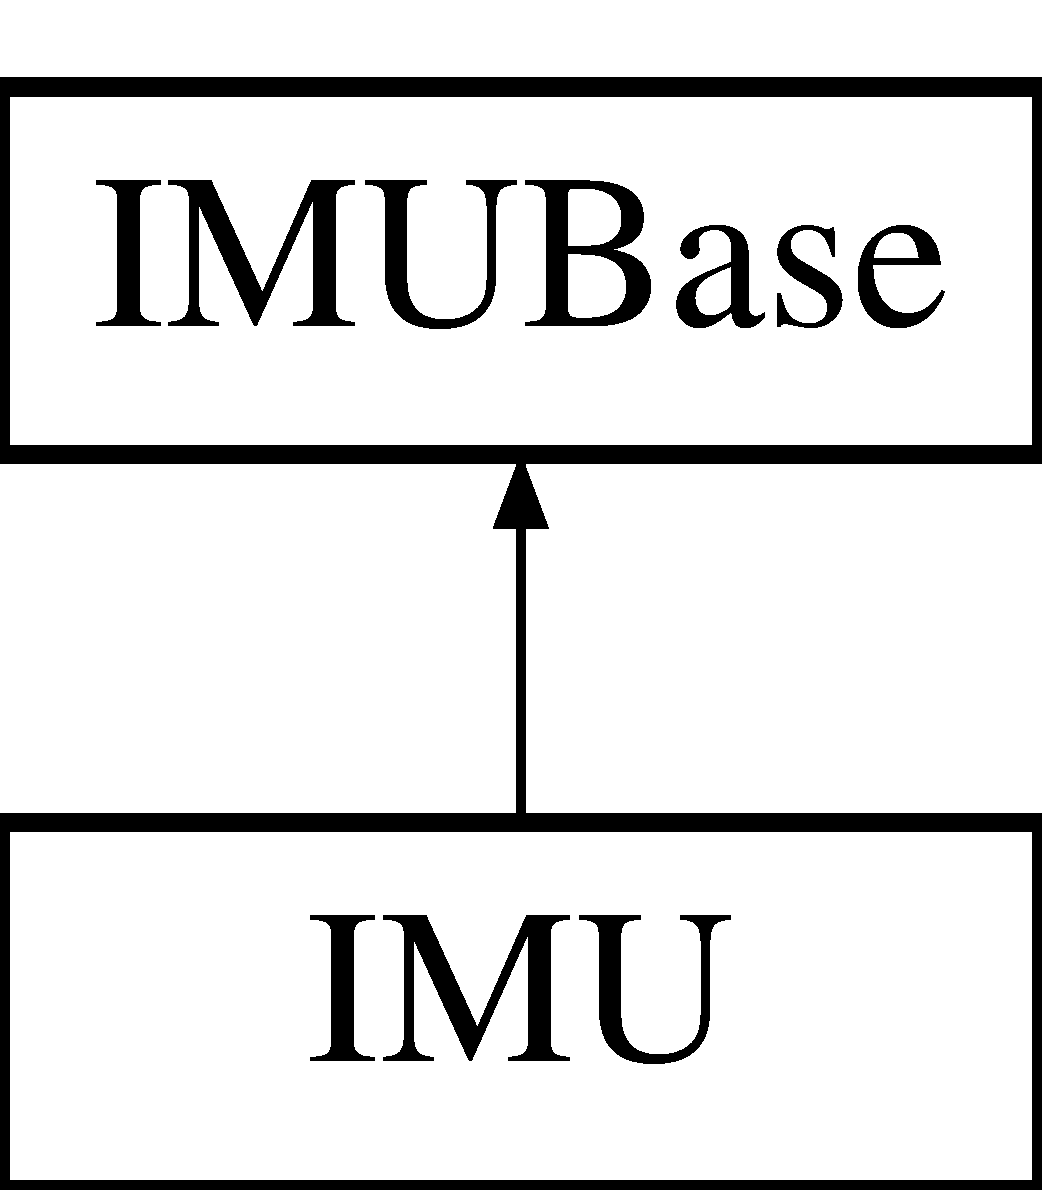
\includegraphics[height=2.000000cm]{class_i_m_u_base}
\end{center}
\end{figure}
\subsubsection*{Public Member Functions}
\begin{DoxyCompactItemize}
\item 
virtual void \hyperlink{class_i_m_u_base_a27fdd96992dfa8867943407fc400d071}{Reset} ()=0
\item 
virtual void \hyperlink{class_i_m_u_base_ad4f6b6562edc0e2b76591d0deca191d7}{SampleRate} (uint16\_\-t)=0
\item 
virtual int \hyperlink{class_i_m_u_base_a74d84beba0da335f49aa7ce94612cf13}{Setup} ()=0
\item 
virtual int \hyperlink{class_i_m_u_base_af31c2ed51cd36cc3230ebbb58757784a}{Start} ()=0
\item 
virtual int \hyperlink{class_i_m_u_base_a5b136166ec3849cbc1f93a13367eb08d}{Stop} ()=0
\item 
virtual int \hyperlink{class_i_m_u_base_a60bf7f5f9728d11bae5ca64bc7a9c10b}{ForceStartStop} ()=0
\item 
virtual bool \hyperlink{class_i_m_u_base_adb8539af8660d291fdde1f38b3d644f3}{Busy} ()=0
\item 
virtual void \hyperlink{class_i_m_u_base_a6e65b709e0212f95299ce9fa464b4651}{ResetTimer} ()=0
\item 
virtual void \hyperlink{class_i_m_u_base_a9b4cc325e9858a8bb204733dc7906ec2}{UseGyro} (bool bEnable)=0
\item 
virtual void \hyperlink{class_i_m_u_base_aa9c09bfd70f81b4a2df20cc5ae1474c3}{NextIMU} (\hyperlink{class_i_m_u_base}{IMUBase} $\ast$)=0
\item 
virtual int \hyperlink{class_i_m_u_base_a55327f28a0ad5e54d94f0c698b04827a}{BeginRead} ()=0
\item 
virtual bool \hyperlink{class_i_m_u_base_a53d56fa29c66935306e1dcca140aa9ff}{DataReady} ()=0
\item 
virtual uint8\_\-t $\ast$ \hyperlink{class_i_m_u_base_a13cf0868e2c3c31838fe889315ccfb0c}{GetPacketData} (uint8\_\-t $\ast$pPacket)=0
\item 
virtual void \hyperlink{class_i_m_u_base_ab920218bb6630f9e91ef7d0f07599203}{CheckIDs} (\hyperlink{class_hardware_serial}{HardwareSerial} $\ast$pSerial)=0
\item 
virtual void \hyperlink{class_i_m_u_base_a78622fbfb40a5bbee5e83bb8a0780d04}{ResetDevices} ()=0
\end{DoxyCompactItemize}


\subsubsection{Detailed Description}


Definition at line \hyperlink{_i_m_u_8h_source_l00016}{16} of file \hyperlink{_i_m_u_8h_source}{IMU.h}.



\subsubsection{Member Function Documentation}
\hypertarget{class_i_m_u_base_a55327f28a0ad5e54d94f0c698b04827a}{
\index{IMUBase@{IMUBase}!BeginRead@{BeginRead}}
\index{BeginRead@{BeginRead}!IMUBase@{IMUBase}}
\paragraph[{BeginRead}]{\setlength{\rightskip}{0pt plus 5cm}virtual int IMUBase::BeginRead (
\begin{DoxyParamCaption}
{}
\end{DoxyParamCaption}
)\hspace{0.3cm}{\ttfamily  \mbox{[}pure virtual\mbox{]}}}\hfill}
\label{class_i_m_u_base_a55327f28a0ad5e54d94f0c698b04827a}


Implemented in \hyperlink{class_i_m_u_a3c949edee15e2f618d7ee263b0a4bcb3}{IMU}.



Referenced by \hyperlink{_i_m_u_8cpp_source_l00108}{IMU::BeginRead()}, and \hyperlink{_i_m_u_8cpp_source_l00348}{IMU::ProcessTransaction()}.

\hypertarget{class_i_m_u_base_adb8539af8660d291fdde1f38b3d644f3}{
\index{IMUBase@{IMUBase}!Busy@{Busy}}
\index{Busy@{Busy}!IMUBase@{IMUBase}}
\paragraph[{Busy}]{\setlength{\rightskip}{0pt plus 5cm}virtual bool IMUBase::Busy (
\begin{DoxyParamCaption}
{}
\end{DoxyParamCaption}
)\hspace{0.3cm}{\ttfamily  \mbox{[}pure virtual\mbox{]}}}\hfill}
\label{class_i_m_u_base_adb8539af8660d291fdde1f38b3d644f3}


Implemented in \hyperlink{class_i_m_u_ade0f7e6be2eda441bfaa2cb372fec55a}{IMU}.

\hypertarget{class_i_m_u_base_ab920218bb6630f9e91ef7d0f07599203}{
\index{IMUBase@{IMUBase}!CheckIDs@{CheckIDs}}
\index{CheckIDs@{CheckIDs}!IMUBase@{IMUBase}}
\paragraph[{CheckIDs}]{\setlength{\rightskip}{0pt plus 5cm}virtual void IMUBase::CheckIDs (
\begin{DoxyParamCaption}
\item[{{\bf HardwareSerial} $\ast$}]{pSerial}
\end{DoxyParamCaption}
)\hspace{0.3cm}{\ttfamily  \mbox{[}pure virtual\mbox{]}}}\hfill}
\label{class_i_m_u_base_ab920218bb6630f9e91ef7d0f07599203}


Implemented in \hyperlink{class_i_m_u_a74feb2946c48a92b251e28ac256d887b}{IMU}.

\hypertarget{class_i_m_u_base_a53d56fa29c66935306e1dcca140aa9ff}{
\index{IMUBase@{IMUBase}!DataReady@{DataReady}}
\index{DataReady@{DataReady}!IMUBase@{IMUBase}}
\paragraph[{DataReady}]{\setlength{\rightskip}{0pt plus 5cm}virtual bool IMUBase::DataReady (
\begin{DoxyParamCaption}
{}
\end{DoxyParamCaption}
)\hspace{0.3cm}{\ttfamily  \mbox{[}pure virtual\mbox{]}}}\hfill}
\label{class_i_m_u_base_a53d56fa29c66935306e1dcca140aa9ff}


Implemented in \hyperlink{class_i_m_u_a078d2f3ad27475c9afcaf09c44886e4c}{IMU}.

\hypertarget{class_i_m_u_base_a60bf7f5f9728d11bae5ca64bc7a9c10b}{
\index{IMUBase@{IMUBase}!ForceStartStop@{ForceStartStop}}
\index{ForceStartStop@{ForceStartStop}!IMUBase@{IMUBase}}
\paragraph[{ForceStartStop}]{\setlength{\rightskip}{0pt plus 5cm}virtual int IMUBase::ForceStartStop (
\begin{DoxyParamCaption}
{}
\end{DoxyParamCaption}
)\hspace{0.3cm}{\ttfamily  \mbox{[}pure virtual\mbox{]}}}\hfill}
\label{class_i_m_u_base_a60bf7f5f9728d11bae5ca64bc7a9c10b}


Implemented in \hyperlink{class_i_m_u_a004d2bb9e6155f45edc9e46bce730644}{IMU}.

\hypertarget{class_i_m_u_base_a13cf0868e2c3c31838fe889315ccfb0c}{
\index{IMUBase@{IMUBase}!GetPacketData@{GetPacketData}}
\index{GetPacketData@{GetPacketData}!IMUBase@{IMUBase}}
\paragraph[{GetPacketData}]{\setlength{\rightskip}{0pt plus 5cm}virtual uint8\_\-t$\ast$ IMUBase::GetPacketData (
\begin{DoxyParamCaption}
\item[{uint8\_\-t $\ast$}]{pPacket}
\end{DoxyParamCaption}
)\hspace{0.3cm}{\ttfamily  \mbox{[}pure virtual\mbox{]}}}\hfill}
\label{class_i_m_u_base_a13cf0868e2c3c31838fe889315ccfb0c}


Implemented in \hyperlink{class_i_m_u_a4f72b7f99fc42f30c9478ba7ed65654e}{IMU}.

\hypertarget{class_i_m_u_base_aa9c09bfd70f81b4a2df20cc5ae1474c3}{
\index{IMUBase@{IMUBase}!NextIMU@{NextIMU}}
\index{NextIMU@{NextIMU}!IMUBase@{IMUBase}}
\paragraph[{NextIMU}]{\setlength{\rightskip}{0pt plus 5cm}virtual void IMUBase::NextIMU (
\begin{DoxyParamCaption}
\item[{{\bf IMUBase} $\ast$}]{}
\end{DoxyParamCaption}
)\hspace{0.3cm}{\ttfamily  \mbox{[}pure virtual\mbox{]}}}\hfill}
\label{class_i_m_u_base_aa9c09bfd70f81b4a2df20cc5ae1474c3}


Implemented in \hyperlink{class_i_m_u_ac46c8e580371cf97e4625dda450f01fd}{IMU}.

\hypertarget{class_i_m_u_base_a27fdd96992dfa8867943407fc400d071}{
\index{IMUBase@{IMUBase}!Reset@{Reset}}
\index{Reset@{Reset}!IMUBase@{IMUBase}}
\paragraph[{Reset}]{\setlength{\rightskip}{0pt plus 5cm}virtual void IMUBase::Reset (
\begin{DoxyParamCaption}
{}
\end{DoxyParamCaption}
)\hspace{0.3cm}{\ttfamily  \mbox{[}pure virtual\mbox{]}}}\hfill}
\label{class_i_m_u_base_a27fdd96992dfa8867943407fc400d071}


Implemented in \hyperlink{class_i_m_u_a13191357ff93d02f6cc7aa7e55b13d67}{IMU}.

\hypertarget{class_i_m_u_base_a78622fbfb40a5bbee5e83bb8a0780d04}{
\index{IMUBase@{IMUBase}!ResetDevices@{ResetDevices}}
\index{ResetDevices@{ResetDevices}!IMUBase@{IMUBase}}
\paragraph[{ResetDevices}]{\setlength{\rightskip}{0pt plus 5cm}virtual void IMUBase::ResetDevices (
\begin{DoxyParamCaption}
{}
\end{DoxyParamCaption}
)\hspace{0.3cm}{\ttfamily  \mbox{[}pure virtual\mbox{]}}}\hfill}
\label{class_i_m_u_base_a78622fbfb40a5bbee5e83bb8a0780d04}


Implemented in \hyperlink{class_i_m_u_a98f9a8244dd1a07f8771450097371b2c}{IMU}.

\hypertarget{class_i_m_u_base_a6e65b709e0212f95299ce9fa464b4651}{
\index{IMUBase@{IMUBase}!ResetTimer@{ResetTimer}}
\index{ResetTimer@{ResetTimer}!IMUBase@{IMUBase}}
\paragraph[{ResetTimer}]{\setlength{\rightskip}{0pt plus 5cm}virtual void IMUBase::ResetTimer (
\begin{DoxyParamCaption}
{}
\end{DoxyParamCaption}
)\hspace{0.3cm}{\ttfamily  \mbox{[}pure virtual\mbox{]}}}\hfill}
\label{class_i_m_u_base_a6e65b709e0212f95299ce9fa464b4651}


Implemented in \hyperlink{class_i_m_u_a187dc9de30f97f5154e0ff904eb6ee1a}{IMU}.

\hypertarget{class_i_m_u_base_ad4f6b6562edc0e2b76591d0deca191d7}{
\index{IMUBase@{IMUBase}!SampleRate@{SampleRate}}
\index{SampleRate@{SampleRate}!IMUBase@{IMUBase}}
\paragraph[{SampleRate}]{\setlength{\rightskip}{0pt plus 5cm}virtual void IMUBase::SampleRate (
\begin{DoxyParamCaption}
\item[{uint16\_\-t}]{}
\end{DoxyParamCaption}
)\hspace{0.3cm}{\ttfamily  \mbox{[}pure virtual\mbox{]}}}\hfill}
\label{class_i_m_u_base_ad4f6b6562edc0e2b76591d0deca191d7}


Implemented in \hyperlink{class_i_m_u_a7705d9d642b093a670e78534c9b2d3db}{IMU}.

\hypertarget{class_i_m_u_base_a74d84beba0da335f49aa7ce94612cf13}{
\index{IMUBase@{IMUBase}!Setup@{Setup}}
\index{Setup@{Setup}!IMUBase@{IMUBase}}
\paragraph[{Setup}]{\setlength{\rightskip}{0pt plus 5cm}virtual int IMUBase::Setup (
\begin{DoxyParamCaption}
{}
\end{DoxyParamCaption}
)\hspace{0.3cm}{\ttfamily  \mbox{[}pure virtual\mbox{]}}}\hfill}
\label{class_i_m_u_base_a74d84beba0da335f49aa7ce94612cf13}


Implemented in \hyperlink{class_i_m_u_a290737d42de965c15c8327edfc516ffd}{IMU}.

\hypertarget{class_i_m_u_base_af31c2ed51cd36cc3230ebbb58757784a}{
\index{IMUBase@{IMUBase}!Start@{Start}}
\index{Start@{Start}!IMUBase@{IMUBase}}
\paragraph[{Start}]{\setlength{\rightskip}{0pt plus 5cm}virtual int IMUBase::Start (
\begin{DoxyParamCaption}
{}
\end{DoxyParamCaption}
)\hspace{0.3cm}{\ttfamily  \mbox{[}pure virtual\mbox{]}}}\hfill}
\label{class_i_m_u_base_af31c2ed51cd36cc3230ebbb58757784a}


Implemented in \hyperlink{class_i_m_u_a7c03f7a423240538756a62441b298d01}{IMU}.

\hypertarget{class_i_m_u_base_a5b136166ec3849cbc1f93a13367eb08d}{
\index{IMUBase@{IMUBase}!Stop@{Stop}}
\index{Stop@{Stop}!IMUBase@{IMUBase}}
\paragraph[{Stop}]{\setlength{\rightskip}{0pt plus 5cm}virtual int IMUBase::Stop (
\begin{DoxyParamCaption}
{}
\end{DoxyParamCaption}
)\hspace{0.3cm}{\ttfamily  \mbox{[}pure virtual\mbox{]}}}\hfill}
\label{class_i_m_u_base_a5b136166ec3849cbc1f93a13367eb08d}


Implemented in \hyperlink{class_i_m_u_af0841bed4167f7a4eb12c40d7b8e615e}{IMU}.

\hypertarget{class_i_m_u_base_a9b4cc325e9858a8bb204733dc7906ec2}{
\index{IMUBase@{IMUBase}!UseGyro@{UseGyro}}
\index{UseGyro@{UseGyro}!IMUBase@{IMUBase}}
\paragraph[{UseGyro}]{\setlength{\rightskip}{0pt plus 5cm}virtual void IMUBase::UseGyro (
\begin{DoxyParamCaption}
\item[{bool}]{bEnable}
\end{DoxyParamCaption}
)\hspace{0.3cm}{\ttfamily  \mbox{[}pure virtual\mbox{]}}}\hfill}
\label{class_i_m_u_base_a9b4cc325e9858a8bb204733dc7906ec2}


Implemented in \hyperlink{class_i_m_u_a86f05be645d2096f0b2b3cfbe8ea0ce8}{IMU}.



The documentation for this class was generated from the following file:\begin{DoxyCompactItemize}
\item 
\hyperlink{_i_m_u_8h}{IMU.h}\end{DoxyCompactItemize}

\hypertarget{class_port}{
\subsection{Port Class Reference}
\label{class_port}\index{Port@{Port}}
}


{\ttfamily \#include $<$Port.h$>$}

\subsubsection*{Public Member Functions}
\begin{DoxyCompactItemize}
\item 
\hyperlink{class_port_a6f90240a1d5bb00b7cb0284134ba3dfc}{Port} (PORT\_\-t $\ast$)
\item 
\hyperlink{class_port_afe166c2a6b10ad34d47472a150366bc1}{$\sim$Port} ()
\item 
void \hyperlink{class_port_a8dd6215565362d65fd4ef159b7b8dc95}{Notify} (\hyperlink{class_port_notify}{PortNotify} $\ast$pClient, uint8\_\-t id)
\item 
void \hyperlink{class_port_ab9841b306c73a2b7a1a7a141da222808}{int0} ()
\item 
void \hyperlink{class_port_ac1ea39cc9b07779045dd218aa2364e25}{int1} ()
\item 
void \hyperlink{class_port_a3c3182388b13059550d19e828959ab37}{SetDir} (uint8\_\-t dir)
\item 
void \hyperlink{class_port_a8edf3efbf5258faa7221109f5cbd5a40}{SetPinsAsInput} (uint8\_\-t mask)
\item 
void \hyperlink{class_port_a15035cc63128ae28294c154527c9d2fe}{SetPinsAsOutput} (uint8\_\-t mask)
\item 
void \hyperlink{class_port_a4c7069d8f3c95c2edbbb5945041c687d}{SetPinsHigh} (uint8\_\-t mask)
\item 
void \hyperlink{class_port_aa0e48b7851cc1352c5e8ddc371351e21}{SetPinsLow} (uint8\_\-t mask)
\item 
uint8\_\-t \hyperlink{class_port_ab13ab1f58e8f17fec681e38872ac56d9}{GetPins} ()
\item 
void \hyperlink{class_port_ae43736d7fff93b93d1d1dac27df64591}{InterruptLevel} (uint8\_\-t num, uint8\_\-t lvl)
\begin{DoxyCompactList}\small\item\em Interrupt control. \item\end{DoxyCompactList}\item 
void \hyperlink{class_port_a638be122540b191c8cb84b61d6363d28}{InterruptMask} (uint8\_\-t num, uint8\_\-t mask)
\item 
void \hyperlink{class_port_ab2f2ecab7c1402a03c87d866a8cd5380}{PinControl} (uint8\_\-t mask, bool bSlewLimit, bool bInverted, PORT\_\-OPC\_\-t OutputConfig, PORT\_\-ISC\_\-t InputSense)
\begin{DoxyCompactList}\small\item\em Pin Control Register. \item\end{DoxyCompactList}\end{DoxyCompactItemize}
\subsubsection*{Protected Attributes}
\begin{DoxyCompactItemize}
\item 
PORT\_\-t $\ast$ \hyperlink{class_port_a1475caa8ec2e667350eae96d4b7a28ac}{\_\-pPort}
\item 
\hyperlink{class_port_notify}{PortNotify} $\ast$ \hyperlink{class_port_ac939fdc751f6e01ce4afcdf97f4598f9}{\_\-pNotifyClient}
\item 
uint8\_\-t \hyperlink{class_port_ac1dae0f3300d4fc57f16f8b548b0e9d7}{\_\-pNotifyID}
\end{DoxyCompactItemize}


\subsubsection{Detailed Description}
Class to handle the setup and control of a port on the ATxmega. This class will setup the port using the PinControl method. It will also setup and receive interrupts on either int0 or int1. You may set an interrupt mask to determine which pins cause which interrupt. For example, it is possible to have pins 0 and 1 cause interrupts on ISR0, and pins 6 and 7 to interrupt on ISR1. 

Definition at line \hyperlink{_port_8h_source_l00026}{26} of file \hyperlink{_port_8h_source}{Port.h}.



\subsubsection{Constructor \& Destructor Documentation}
\hypertarget{class_port_a6f90240a1d5bb00b7cb0284134ba3dfc}{
\index{Port@{Port}!Port@{Port}}
\index{Port@{Port}!Port@{Port}}
\paragraph[{Port}]{\setlength{\rightskip}{0pt plus 5cm}Port::Port (
\begin{DoxyParamCaption}
\item[{PORT\_\-t $\ast$}]{pPort}
\end{DoxyParamCaption}
)}\hfill}
\label{class_port_a6f90240a1d5bb00b7cb0284134ba3dfc}


Definition at line \hyperlink{_port_8cpp_source_l00058}{58} of file \hyperlink{_port_8cpp_source}{Port.cpp}.



References \hyperlink{_port_8h_source_l00029}{\_\-pPort}, and \hyperlink{_port_8cpp_source_l00033}{SetPointer()}.


\begin{DoxyCode}
\{
    \hyperlink{class_port_a1475caa8ec2e667350eae96d4b7a28ac}{_pPort} = pPort;
    \hyperlink{_port_8cpp_afaf5d589e6cb241cd3822efd8c9cbb05}{SetPointer}(\hyperlink{class_port_a1475caa8ec2e667350eae96d4b7a28ac}{_pPort},\textcolor{keyword}{this});
\}
\end{DoxyCode}
\hypertarget{class_port_afe166c2a6b10ad34d47472a150366bc1}{
\index{Port@{Port}!$\sim$Port@{$\sim$Port}}
\index{$\sim$Port@{$\sim$Port}!Port@{Port}}
\paragraph[{$\sim$Port}]{\setlength{\rightskip}{0pt plus 5cm}Port::$\sim$Port (
\begin{DoxyParamCaption}
{}
\end{DoxyParamCaption}
)}\hfill}
\label{class_port_afe166c2a6b10ad34d47472a150366bc1}


Definition at line \hyperlink{_port_8cpp_source_l00064}{64} of file \hyperlink{_port_8cpp_source}{Port.cpp}.



References \hyperlink{_port_8h_source_l00029}{\_\-pPort}, and \hyperlink{_port_8cpp_source_l00033}{SetPointer()}.


\begin{DoxyCode}
\{
    \hyperlink{_port_8cpp_afaf5d589e6cb241cd3822efd8c9cbb05}{SetPointer}(\hyperlink{class_port_a1475caa8ec2e667350eae96d4b7a28ac}{_pPort},0);
\}
\end{DoxyCode}


\subsubsection{Member Function Documentation}
\hypertarget{class_port_ab13ab1f58e8f17fec681e38872ac56d9}{
\index{Port@{Port}!GetPins@{GetPins}}
\index{GetPins@{GetPins}!Port@{Port}}
\paragraph[{GetPins}]{\setlength{\rightskip}{0pt plus 5cm}uint8\_\-t Port::GetPins (
\begin{DoxyParamCaption}
{}
\end{DoxyParamCaption}
)}\hfill}
\label{class_port_ab13ab1f58e8f17fec681e38872ac56d9}


Definition at line \hyperlink{_port_8cpp_source_l00116}{116} of file \hyperlink{_port_8cpp_source}{Port.cpp}.



References \hyperlink{_port_8h_source_l00029}{\_\-pPort}.


\begin{DoxyCode}
\{
    \textcolor{keywordflow}{return} \hyperlink{class_port_a1475caa8ec2e667350eae96d4b7a28ac}{_pPort}->IN;
\}
\end{DoxyCode}
\hypertarget{class_port_ab9841b306c73a2b7a1a7a141da222808}{
\index{Port@{Port}!int0@{int0}}
\index{int0@{int0}!Port@{Port}}
\paragraph[{int0}]{\setlength{\rightskip}{0pt plus 5cm}void Port::int0 (
\begin{DoxyParamCaption}
{}
\end{DoxyParamCaption}
)}\hfill}
\label{class_port_ab9841b306c73a2b7a1a7a141da222808}


Definition at line \hyperlink{_port_8cpp_source_l00075}{75} of file \hyperlink{_port_8cpp_source}{Port.cpp}.



References \hyperlink{_port_8h_source_l00030}{\_\-pNotifyClient}, \hyperlink{_port_8h_source_l00031}{\_\-pNotifyID}, \hyperlink{_port_8h_source_l00029}{\_\-pPort}, and \hyperlink{class_port_notify_a56e1550c6c2d0602fe523c2a3b648f85}{PortNotify::PortISR0()}.


\begin{DoxyCode}
\{
    \textcolor{keywordflow}{if} (\hyperlink{class_port_ac939fdc751f6e01ce4afcdf97f4598f9}{_pNotifyClient}) \{
        \hyperlink{class_port_ac939fdc751f6e01ce4afcdf97f4598f9}{_pNotifyClient}->\hyperlink{class_port_notify_a56e1550c6c2d0602fe523c2a3b648f85}{PortISR0}(\hyperlink{class_port_ac1dae0f3300d4fc57f16f8b548b0e9d7}{_pNotifyID});
    \}
    \hyperlink{class_port_a1475caa8ec2e667350eae96d4b7a28ac}{_pPort}->INTFLAGS = 0x1;
\}
\end{DoxyCode}
\hypertarget{class_port_ac1ea39cc9b07779045dd218aa2364e25}{
\index{Port@{Port}!int1@{int1}}
\index{int1@{int1}!Port@{Port}}
\paragraph[{int1}]{\setlength{\rightskip}{0pt plus 5cm}void Port::int1 (
\begin{DoxyParamCaption}
{}
\end{DoxyParamCaption}
)}\hfill}
\label{class_port_ac1ea39cc9b07779045dd218aa2364e25}


Definition at line \hyperlink{_port_8cpp_source_l00083}{83} of file \hyperlink{_port_8cpp_source}{Port.cpp}.



References \hyperlink{_port_8h_source_l00030}{\_\-pNotifyClient}, \hyperlink{_port_8h_source_l00031}{\_\-pNotifyID}, \hyperlink{_port_8h_source_l00029}{\_\-pPort}, and \hyperlink{class_port_notify_a8f9f4a14e41092147194fb9cba192de8}{PortNotify::PortISR1()}.


\begin{DoxyCode}
\{
    \textcolor{keywordflow}{if} (\hyperlink{class_port_ac939fdc751f6e01ce4afcdf97f4598f9}{_pNotifyClient}) \{
        \hyperlink{class_port_ac939fdc751f6e01ce4afcdf97f4598f9}{_pNotifyClient}->\hyperlink{class_port_notify_a8f9f4a14e41092147194fb9cba192de8}{PortISR1}(\hyperlink{class_port_ac1dae0f3300d4fc57f16f8b548b0e9d7}{_pNotifyID});
    \}
    \hyperlink{class_port_a1475caa8ec2e667350eae96d4b7a28ac}{_pPort}->INTFLAGS = 0x2;
\}
\end{DoxyCode}
\hypertarget{class_port_ae43736d7fff93b93d1d1dac27df64591}{
\index{Port@{Port}!InterruptLevel@{InterruptLevel}}
\index{InterruptLevel@{InterruptLevel}!Port@{Port}}
\paragraph[{InterruptLevel}]{\setlength{\rightskip}{0pt plus 5cm}void Port::InterruptLevel (
\begin{DoxyParamCaption}
\item[{uint8\_\-t}]{num, }
\item[{uint8\_\-t}]{lvl}
\end{DoxyParamCaption}
)}\hfill}
\label{class_port_ae43736d7fff93b93d1d1dac27df64591}


Interrupt control. 



Definition at line \hyperlink{_port_8cpp_source_l00121}{121} of file \hyperlink{_port_8cpp_source}{Port.cpp}.



References \hyperlink{_port_8h_source_l00029}{\_\-pPort}.


\begin{DoxyCode}
\{
    \textcolor{keywordflow}{if} (num == 0) \{
        \hyperlink{class_port_a1475caa8ec2e667350eae96d4b7a28ac}{_pPort}->INTCTRL &= ~(0x3);
        \hyperlink{class_port_a1475caa8ec2e667350eae96d4b7a28ac}{_pPort}->INTCTRL |= (lvl & 0x3);
    \} \textcolor{keywordflow}{else} \{
        \hyperlink{class_port_a1475caa8ec2e667350eae96d4b7a28ac}{_pPort}->INTCTRL &= ~(0xC);
        \hyperlink{class_port_a1475caa8ec2e667350eae96d4b7a28ac}{_pPort}->INTCTRL |= (lvl & 0x3) << 2;
    \}
\}
\end{DoxyCode}
\hypertarget{class_port_a638be122540b191c8cb84b61d6363d28}{
\index{Port@{Port}!InterruptMask@{InterruptMask}}
\index{InterruptMask@{InterruptMask}!Port@{Port}}
\paragraph[{InterruptMask}]{\setlength{\rightskip}{0pt plus 5cm}void Port::InterruptMask (
\begin{DoxyParamCaption}
\item[{uint8\_\-t}]{num, }
\item[{uint8\_\-t}]{mask}
\end{DoxyParamCaption}
)}\hfill}
\label{class_port_a638be122540b191c8cb84b61d6363d28}


Definition at line \hyperlink{_port_8cpp_source_l00132}{132} of file \hyperlink{_port_8cpp_source}{Port.cpp}.



References \hyperlink{_port_8h_source_l00029}{\_\-pPort}.


\begin{DoxyCode}
\{
    \textcolor{keywordflow}{if} (num == 0) \{
        \hyperlink{class_port_a1475caa8ec2e667350eae96d4b7a28ac}{_pPort}->INT0MASK = mask;
    \} \textcolor{keywordflow}{else} \{
        \hyperlink{class_port_a1475caa8ec2e667350eae96d4b7a28ac}{_pPort}->INT1MASK = mask;
    \}
\}
\end{DoxyCode}
\hypertarget{class_port_a8dd6215565362d65fd4ef159b7b8dc95}{
\index{Port@{Port}!Notify@{Notify}}
\index{Notify@{Notify}!Port@{Port}}
\paragraph[{Notify}]{\setlength{\rightskip}{0pt plus 5cm}void Port::Notify (
\begin{DoxyParamCaption}
\item[{{\bf PortNotify} $\ast$}]{pClient, }
\item[{uint8\_\-t}]{id}
\end{DoxyParamCaption}
)}\hfill}
\label{class_port_a8dd6215565362d65fd4ef159b7b8dc95}


Definition at line \hyperlink{_port_8cpp_source_l00069}{69} of file \hyperlink{_port_8cpp_source}{Port.cpp}.



References \hyperlink{_port_8h_source_l00030}{\_\-pNotifyClient}, and \hyperlink{_port_8h_source_l00031}{\_\-pNotifyID}.


\begin{DoxyCode}
\{
    \hyperlink{class_port_ac939fdc751f6e01ce4afcdf97f4598f9}{_pNotifyClient}  = pClient;
    \hyperlink{class_port_ac1dae0f3300d4fc57f16f8b548b0e9d7}{_pNotifyID}      = id;
\}
\end{DoxyCode}
\hypertarget{class_port_ab2f2ecab7c1402a03c87d866a8cd5380}{
\index{Port@{Port}!PinControl@{PinControl}}
\index{PinControl@{PinControl}!Port@{Port}}
\paragraph[{PinControl}]{\setlength{\rightskip}{0pt plus 5cm}void Port::PinControl (
\begin{DoxyParamCaption}
\item[{uint8\_\-t}]{mask, }
\item[{bool}]{bSlewLimit, }
\item[{bool}]{bInverted, }
\item[{PORT\_\-OPC\_\-t}]{OutputConfig, }
\item[{PORT\_\-ISC\_\-t}]{InputSense}
\end{DoxyParamCaption}
)}\hfill}
\label{class_port_ab2f2ecab7c1402a03c87d866a8cd5380}


Pin Control Register. 



The MPCMASK is a neat feature. I set each of the bits of the mask high, then configure any of the PINxCTRL registers, and only the pins specified in the mask get configured. Also, they all get the same config, so it's faster. It does not matter if I am actually configuring pin 0 or not, even though I specify PN0CTRL. 



Definition at line \hyperlink{_port_8cpp_source_l00141}{141} of file \hyperlink{_port_8cpp_source}{Port.cpp}.



References \hyperlink{_port_8h_source_l00029}{\_\-pPort}.


\begin{DoxyCode}
\{
    PORTCFG.MPCMASK = mask;
    \hyperlink{class_port_a1475caa8ec2e667350eae96d4b7a28ac}{_pPort}->PIN0CTRL = 
        (bSlewLimit ? 0x80 : 0x0) |
        (bInverted ? 0x40 : 0x0)  |
        OutputConfig | 
        InputSense
        ;
\}
\end{DoxyCode}
\hypertarget{class_port_a3c3182388b13059550d19e828959ab37}{
\index{Port@{Port}!SetDir@{SetDir}}
\index{SetDir@{SetDir}!Port@{Port}}
\paragraph[{SetDir}]{\setlength{\rightskip}{0pt plus 5cm}void Port::SetDir (
\begin{DoxyParamCaption}
\item[{uint8\_\-t}]{dir}
\end{DoxyParamCaption}
)}\hfill}
\label{class_port_a3c3182388b13059550d19e828959ab37}


Definition at line \hyperlink{_port_8cpp_source_l00091}{91} of file \hyperlink{_port_8cpp_source}{Port.cpp}.



References \hyperlink{_port_8h_source_l00029}{\_\-pPort}.


\begin{DoxyCode}
\{
    \hyperlink{class_port_a1475caa8ec2e667350eae96d4b7a28ac}{_pPort}->DIR = dir;
\}
\end{DoxyCode}
\hypertarget{class_port_a8edf3efbf5258faa7221109f5cbd5a40}{
\index{Port@{Port}!SetPinsAsInput@{SetPinsAsInput}}
\index{SetPinsAsInput@{SetPinsAsInput}!Port@{Port}}
\paragraph[{SetPinsAsInput}]{\setlength{\rightskip}{0pt plus 5cm}void Port::SetPinsAsInput (
\begin{DoxyParamCaption}
\item[{uint8\_\-t}]{mask}
\end{DoxyParamCaption}
)}\hfill}
\label{class_port_a8edf3efbf5258faa7221109f5cbd5a40}


Definition at line \hyperlink{_port_8cpp_source_l00096}{96} of file \hyperlink{_port_8cpp_source}{Port.cpp}.



References \hyperlink{_port_8h_source_l00029}{\_\-pPort}.


\begin{DoxyCode}
\{
    \hyperlink{class_port_a1475caa8ec2e667350eae96d4b7a28ac}{_pPort}->DIRCLR = mask;
\}
\end{DoxyCode}
\hypertarget{class_port_a15035cc63128ae28294c154527c9d2fe}{
\index{Port@{Port}!SetPinsAsOutput@{SetPinsAsOutput}}
\index{SetPinsAsOutput@{SetPinsAsOutput}!Port@{Port}}
\paragraph[{SetPinsAsOutput}]{\setlength{\rightskip}{0pt plus 5cm}void Port::SetPinsAsOutput (
\begin{DoxyParamCaption}
\item[{uint8\_\-t}]{mask}
\end{DoxyParamCaption}
)}\hfill}
\label{class_port_a15035cc63128ae28294c154527c9d2fe}


Definition at line \hyperlink{_port_8cpp_source_l00101}{101} of file \hyperlink{_port_8cpp_source}{Port.cpp}.



References \hyperlink{_port_8h_source_l00029}{\_\-pPort}.


\begin{DoxyCode}
\{
    \hyperlink{class_port_a1475caa8ec2e667350eae96d4b7a28ac}{_pPort}->DIRSET = mask;
\}
\end{DoxyCode}
\hypertarget{class_port_a4c7069d8f3c95c2edbbb5945041c687d}{
\index{Port@{Port}!SetPinsHigh@{SetPinsHigh}}
\index{SetPinsHigh@{SetPinsHigh}!Port@{Port}}
\paragraph[{SetPinsHigh}]{\setlength{\rightskip}{0pt plus 5cm}void Port::SetPinsHigh (
\begin{DoxyParamCaption}
\item[{uint8\_\-t}]{mask}
\end{DoxyParamCaption}
)}\hfill}
\label{class_port_a4c7069d8f3c95c2edbbb5945041c687d}


Definition at line \hyperlink{_port_8cpp_source_l00106}{106} of file \hyperlink{_port_8cpp_source}{Port.cpp}.



References \hyperlink{_port_8h_source_l00029}{\_\-pPort}.


\begin{DoxyCode}
\{
    \hyperlink{class_port_a1475caa8ec2e667350eae96d4b7a28ac}{_pPort}->OUTSET = mask;
\}
\end{DoxyCode}
\hypertarget{class_port_aa0e48b7851cc1352c5e8ddc371351e21}{
\index{Port@{Port}!SetPinsLow@{SetPinsLow}}
\index{SetPinsLow@{SetPinsLow}!Port@{Port}}
\paragraph[{SetPinsLow}]{\setlength{\rightskip}{0pt plus 5cm}void Port::SetPinsLow (
\begin{DoxyParamCaption}
\item[{uint8\_\-t}]{mask}
\end{DoxyParamCaption}
)}\hfill}
\label{class_port_aa0e48b7851cc1352c5e8ddc371351e21}


Definition at line \hyperlink{_port_8cpp_source_l00111}{111} of file \hyperlink{_port_8cpp_source}{Port.cpp}.



References \hyperlink{_port_8h_source_l00029}{\_\-pPort}.


\begin{DoxyCode}
\{
    \hyperlink{class_port_a1475caa8ec2e667350eae96d4b7a28ac}{_pPort}->OUTCLR = mask;
\}
\end{DoxyCode}


\subsubsection{Member Data Documentation}
\hypertarget{class_port_ac939fdc751f6e01ce4afcdf97f4598f9}{
\index{Port@{Port}!\_\-pNotifyClient@{\_\-pNotifyClient}}
\index{\_\-pNotifyClient@{\_\-pNotifyClient}!Port@{Port}}
\paragraph[{\_\-pNotifyClient}]{\setlength{\rightskip}{0pt plus 5cm}{\bf PortNotify}$\ast$ {\bf Port::\_\-pNotifyClient}\hspace{0.3cm}{\ttfamily  \mbox{[}protected\mbox{]}}}\hfill}
\label{class_port_ac939fdc751f6e01ce4afcdf97f4598f9}


Definition at line \hyperlink{_port_8h_source_l00030}{30} of file \hyperlink{_port_8h_source}{Port.h}.



Referenced by \hyperlink{_port_8cpp_source_l00075}{int0()}, \hyperlink{_port_8cpp_source_l00083}{int1()}, and \hyperlink{_port_8cpp_source_l00069}{Notify()}.

\hypertarget{class_port_ac1dae0f3300d4fc57f16f8b548b0e9d7}{
\index{Port@{Port}!\_\-pNotifyID@{\_\-pNotifyID}}
\index{\_\-pNotifyID@{\_\-pNotifyID}!Port@{Port}}
\paragraph[{\_\-pNotifyID}]{\setlength{\rightskip}{0pt plus 5cm}uint8\_\-t {\bf Port::\_\-pNotifyID}\hspace{0.3cm}{\ttfamily  \mbox{[}protected\mbox{]}}}\hfill}
\label{class_port_ac1dae0f3300d4fc57f16f8b548b0e9d7}


Definition at line \hyperlink{_port_8h_source_l00031}{31} of file \hyperlink{_port_8h_source}{Port.h}.



Referenced by \hyperlink{_port_8cpp_source_l00075}{int0()}, \hyperlink{_port_8cpp_source_l00083}{int1()}, and \hyperlink{_port_8cpp_source_l00069}{Notify()}.

\hypertarget{class_port_a1475caa8ec2e667350eae96d4b7a28ac}{
\index{Port@{Port}!\_\-pPort@{\_\-pPort}}
\index{\_\-pPort@{\_\-pPort}!Port@{Port}}
\paragraph[{\_\-pPort}]{\setlength{\rightskip}{0pt plus 5cm}PORT\_\-t$\ast$ {\bf Port::\_\-pPort}\hspace{0.3cm}{\ttfamily  \mbox{[}protected\mbox{]}}}\hfill}
\label{class_port_a1475caa8ec2e667350eae96d4b7a28ac}


Definition at line \hyperlink{_port_8h_source_l00029}{29} of file \hyperlink{_port_8h_source}{Port.h}.



Referenced by \hyperlink{_port_8cpp_source_l00116}{GetPins()}, \hyperlink{_port_8cpp_source_l00075}{int0()}, \hyperlink{_port_8cpp_source_l00083}{int1()}, \hyperlink{_port_8cpp_source_l00121}{InterruptLevel()}, \hyperlink{_port_8cpp_source_l00132}{InterruptMask()}, \hyperlink{_port_8cpp_source_l00141}{PinControl()}, \hyperlink{_port_8cpp_source_l00058}{Port()}, \hyperlink{_port_8cpp_source_l00091}{SetDir()}, \hyperlink{_port_8cpp_source_l00096}{SetPinsAsInput()}, \hyperlink{_port_8cpp_source_l00101}{SetPinsAsOutput()}, \hyperlink{_port_8cpp_source_l00106}{SetPinsHigh()}, \hyperlink{_port_8cpp_source_l00111}{SetPinsLow()}, and \hyperlink{_port_8cpp_source_l00064}{$\sim$Port()}.



The documentation for this class was generated from the following files:\begin{DoxyCompactItemize}
\item 
\hyperlink{_port_8h}{Port.h}\item 
\hyperlink{_port_8cpp}{Port.cpp}\end{DoxyCompactItemize}

\hypertarget{class_port_notify}{
\subsection{PortNotify Class Reference}
\label{class_port_notify}\index{PortNotify@{PortNotify}}
}


{\ttfamily \#include $<$Port.h$>$}

\subsubsection*{Public Member Functions}
\begin{DoxyCompactItemize}
\item 
virtual void \hyperlink{class_port_notify_a56e1550c6c2d0602fe523c2a3b648f85}{PortISR0} (uint8\_\-t id)=0
\item 
virtual void \hyperlink{class_port_notify_a8f9f4a14e41092147194fb9cba192de8}{PortISR1} (uint8\_\-t id)=0
\end{DoxyCompactItemize}


\subsubsection{Detailed Description}
Base class for any classes that require port change notification If a class requires notification of a port change event, then use this class as a base class. Call the Notify method of any \hyperlink{class_port}{Port} class and pass in the 'this' pointer of the class to notify. Also pass in an index value. The index value is needed becuase it is possible for a single class to request notifications from 2 or more Ports. In order to know which of the ports is sending the notification, use a unique index for both. The actual value of the index is not important. 

Definition at line \hyperlink{_port_8h_source_l00013}{13} of file \hyperlink{_port_8h_source}{Port.h}.



\subsubsection{Member Function Documentation}
\hypertarget{class_port_notify_a56e1550c6c2d0602fe523c2a3b648f85}{
\index{PortNotify@{PortNotify}!PortISR0@{PortISR0}}
\index{PortISR0@{PortISR0}!PortNotify@{PortNotify}}
\paragraph[{PortISR0}]{\setlength{\rightskip}{0pt plus 5cm}virtual void PortNotify::PortISR0 (
\begin{DoxyParamCaption}
\item[{uint8\_\-t}]{id}
\end{DoxyParamCaption}
)\hspace{0.3cm}{\ttfamily  \mbox{[}pure virtual\mbox{]}}}\hfill}
\label{class_port_notify_a56e1550c6c2d0602fe523c2a3b648f85}


Referenced by \hyperlink{_port_8cpp_source_l00075}{Port::int0()}.

\hypertarget{class_port_notify_a8f9f4a14e41092147194fb9cba192de8}{
\index{PortNotify@{PortNotify}!PortISR1@{PortISR1}}
\index{PortISR1@{PortISR1}!PortNotify@{PortNotify}}
\paragraph[{PortISR1}]{\setlength{\rightskip}{0pt plus 5cm}virtual void PortNotify::PortISR1 (
\begin{DoxyParamCaption}
\item[{uint8\_\-t}]{id}
\end{DoxyParamCaption}
)\hspace{0.3cm}{\ttfamily  \mbox{[}pure virtual\mbox{]}}}\hfill}
\label{class_port_notify_a8f9f4a14e41092147194fb9cba192de8}


Referenced by \hyperlink{_port_8cpp_source_l00083}{Port::int1()}.



The documentation for this class was generated from the following file:\begin{DoxyCompactItemize}
\item 
\hyperlink{_port_8h}{Port.h}\end{DoxyCompactItemize}

\hypertarget{class_print}{
\section{Print Class Reference}
\label{class_print}\index{Print@{Print}}
}


{\ttfamily \#include $<$Print.h$>$}

Inheritance diagram for Print:\begin{figure}[H]
\begin{center}
\leavevmode
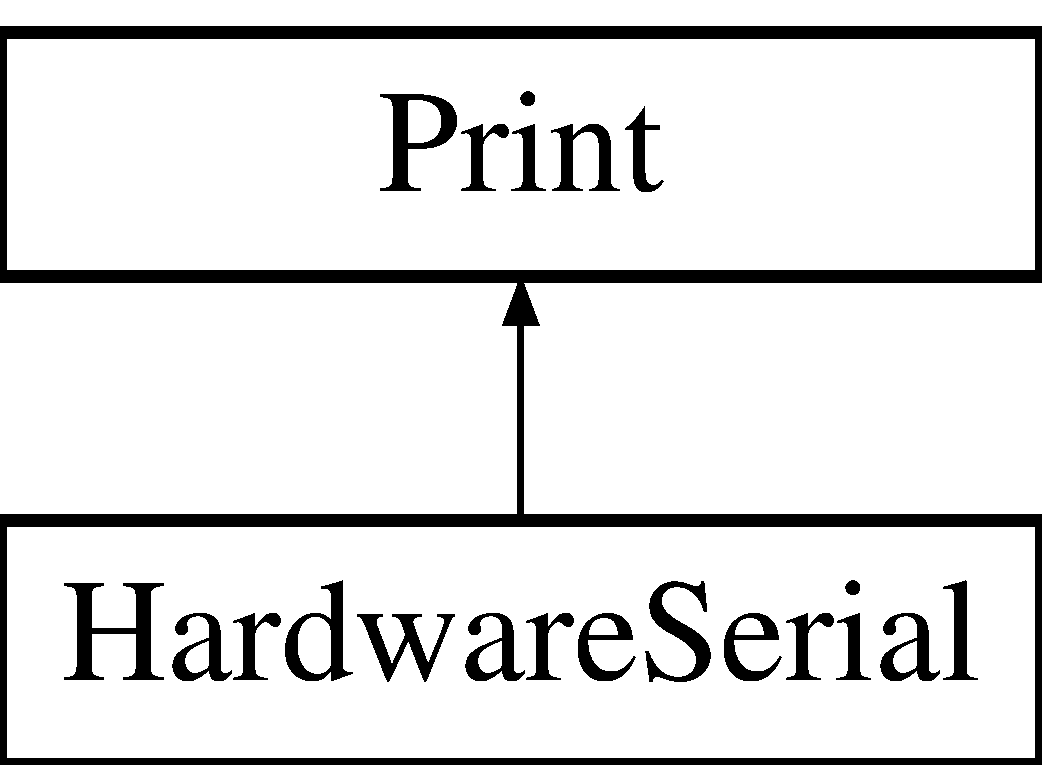
\includegraphics[height=2.000000cm]{class_print}
\end{center}
\end{figure}
\subsection*{Public Member Functions}
\begin{DoxyCompactItemize}
\item 
virtual void \hyperlink{class_print_ad9393033793cfc17f3e37202ba244892}{write} (uint8\_\-t)=0
\item 
virtual void \hyperlink{class_print_ae083258d224bae2e5d8a27a4f8338880}{write} (const char $\ast$str)
\item 
virtual void \hyperlink{class_print_a03094428e21f210e59cc1be63353225d}{write} (const uint8\_\-t $\ast$\hyperlink{_i_m_u_manager_8cpp_a858e0513a46bec1d794f9487c41a969d}{buffer}, size\_\-t size)
\item 
void \hyperlink{class_print_aa7b0a6dc63e3d27effd8459e3d443b83}{print} (const char\mbox{[}$\,$\mbox{]})
\item 
void \hyperlink{class_print_ada24638921c2e86e13c5939c94cf67db}{print} (char, int=BYTE)
\item 
void \hyperlink{class_print_ad7778084a6fe96551d2ec9ce532c5164}{print} (unsigned char, int=BYTE)
\item 
void \hyperlink{class_print_a35a6196999c85e5afc5fd852d088e886}{print} (int, int=DEC)
\item 
void \hyperlink{class_print_a5f8df5d4f941b411ce9d660b48996bea}{print} (unsigned int, int=DEC)
\item 
void \hyperlink{class_print_afab3f8d07a58a8d37fec32d7fcb67b56}{print} (long, int=DEC)
\item 
void \hyperlink{class_print_a4be58e920bdddcaf5496d0ba2ae4ea81}{print} (unsigned long, int=DEC)
\item 
void \hyperlink{class_print_aa5fe80d3a3e8d2dc64f346eb08dcb43f}{print} (double, int=2)
\item 
void \hyperlink{class_print_a09db74a8d51c6b2420c478267f958a51}{println} (const char\mbox{[}$\,$\mbox{]})
\item 
void \hyperlink{class_print_a49bbefc9016ddda486edf3dddaaa07e9}{println} (char, int=BYTE)
\item 
void \hyperlink{class_print_a4eaaf09c278a5927ba2ddcffb6b01e64}{println} (unsigned char, int=BYTE)
\item 
void \hyperlink{class_print_a350bdfe3569acb05a2fdefb7c54e292d}{println} (int, int=DEC)
\item 
void \hyperlink{class_print_af0aeb581689c6e9c9f8331b342a91e20}{println} (unsigned int, int=DEC)
\item 
void \hyperlink{class_print_a1999020b07369721caa16c52fdba4341}{println} (long, int=DEC)
\item 
void \hyperlink{class_print_aacf64fb9630526fb6c666f038a9dc4e6}{println} (unsigned long, int=DEC)
\item 
void \hyperlink{class_print_a4302b58946b9355b0491118227beed07}{println} (double, int=2)
\item 
void \hyperlink{class_print_a525b37c566658ff8113a067f6e8d5bf1}{println} (void)
\end{DoxyCompactItemize}
\subsection*{Private Member Functions}
\begin{DoxyCompactItemize}
\item 
void \hyperlink{class_print_ae6dc349a48650e771a4443e93bfa9c65}{printNumber} (unsigned long, uint8\_\-t)
\item 
void \hyperlink{class_print_afd7abd9d94aa5210d2d0f97e614e4625}{printFloat} (double, uint8\_\-t)
\end{DoxyCompactItemize}


\subsection{Detailed Description}


Definition at line 32 of file Print.h.



\subsection{Member Function Documentation}
\hypertarget{class_print_aa7b0a6dc63e3d27effd8459e3d443b83}{
\index{Print@{Print}!print@{print}}
\index{print@{print}!Print@{Print}}
\subsubsection[{print}]{\setlength{\rightskip}{0pt plus 5cm}void Print::print (
\begin{DoxyParamCaption}
\item[{const char}]{str\mbox{[}$\,$\mbox{]}}
\end{DoxyParamCaption}
)}}
\label{class_print_aa7b0a6dc63e3d27effd8459e3d443b83}


Definition at line 45 of file Print.cpp.



References write().



Referenced by IMU::CheckIDs(), FifoTest(), main(), print(), printFloat(), println(), printNumber(), IMU::Setup(), and IMU::WrAsync().


\begin{DoxyCode}
{
  write(str);
}
\end{DoxyCode}
\hypertarget{class_print_ad7778084a6fe96551d2ec9ce532c5164}{
\index{Print@{Print}!print@{print}}
\index{print@{print}!Print@{Print}}
\subsubsection[{print}]{\setlength{\rightskip}{0pt plus 5cm}void Print::print (
\begin{DoxyParamCaption}
\item[{unsigned char}]{b, }
\item[{int}]{base = {\ttfamily BYTE}}
\end{DoxyParamCaption}
)}}
\label{class_print_ad7778084a6fe96551d2ec9ce532c5164}


Definition at line 55 of file Print.cpp.



References print().


\begin{DoxyCode}
{
  print((unsigned long) b, base);
}
\end{DoxyCode}
\hypertarget{class_print_a35a6196999c85e5afc5fd852d088e886}{
\index{Print@{Print}!print@{print}}
\index{print@{print}!Print@{Print}}
\subsubsection[{print}]{\setlength{\rightskip}{0pt plus 5cm}void Print::print (
\begin{DoxyParamCaption}
\item[{int}]{n, }
\item[{int}]{base = {\ttfamily DEC}}
\end{DoxyParamCaption}
)}}
\label{class_print_a35a6196999c85e5afc5fd852d088e886}


Definition at line 60 of file Print.cpp.



References print().


\begin{DoxyCode}
{
  print((long) n, base);
}
\end{DoxyCode}
\hypertarget{class_print_a5f8df5d4f941b411ce9d660b48996bea}{
\index{Print@{Print}!print@{print}}
\index{print@{print}!Print@{Print}}
\subsubsection[{print}]{\setlength{\rightskip}{0pt plus 5cm}void Print::print (
\begin{DoxyParamCaption}
\item[{unsigned int}]{n, }
\item[{int}]{base = {\ttfamily DEC}}
\end{DoxyParamCaption}
)}}
\label{class_print_a5f8df5d4f941b411ce9d660b48996bea}


Definition at line 65 of file Print.cpp.



References print().


\begin{DoxyCode}
{
  print((unsigned long) n, base);
}
\end{DoxyCode}
\hypertarget{class_print_afab3f8d07a58a8d37fec32d7fcb67b56}{
\index{Print@{Print}!print@{print}}
\index{print@{print}!Print@{Print}}
\subsubsection[{print}]{\setlength{\rightskip}{0pt plus 5cm}void Print::print (
\begin{DoxyParamCaption}
\item[{long}]{n, }
\item[{int}]{base = {\ttfamily DEC}}
\end{DoxyParamCaption}
)}}
\label{class_print_afab3f8d07a58a8d37fec32d7fcb67b56}


Definition at line 70 of file Print.cpp.



References print(), printNumber(), and write().


\begin{DoxyCode}
{
  if (base == 0) {
    write(n);
  } else if (base == 10) {
    if (n < 0) {
      print('-');
      n = -n;
    }
    printNumber(n, 10);
  } else {
    printNumber(n, base);
  }
}
\end{DoxyCode}
\hypertarget{class_print_ada24638921c2e86e13c5939c94cf67db}{
\index{Print@{Print}!print@{print}}
\index{print@{print}!Print@{Print}}
\subsubsection[{print}]{\setlength{\rightskip}{0pt plus 5cm}void Print::print (
\begin{DoxyParamCaption}
\item[{char}]{c, }
\item[{int}]{base = {\ttfamily BYTE}}
\end{DoxyParamCaption}
)}}
\label{class_print_ada24638921c2e86e13c5939c94cf67db}


Definition at line 50 of file Print.cpp.



References print().


\begin{DoxyCode}
{
  print((long) c, base);
}
\end{DoxyCode}
\hypertarget{class_print_a4be58e920bdddcaf5496d0ba2ae4ea81}{
\index{Print@{Print}!print@{print}}
\index{print@{print}!Print@{Print}}
\subsubsection[{print}]{\setlength{\rightskip}{0pt plus 5cm}void Print::print (
\begin{DoxyParamCaption}
\item[{unsigned long}]{n, }
\item[{int}]{base = {\ttfamily DEC}}
\end{DoxyParamCaption}
)}}
\label{class_print_a4be58e920bdddcaf5496d0ba2ae4ea81}


Definition at line 85 of file Print.cpp.



References printNumber(), and write().


\begin{DoxyCode}
{
  if (base == 0) write(n);
  else printNumber(n, base);
}
\end{DoxyCode}
\hypertarget{class_print_aa5fe80d3a3e8d2dc64f346eb08dcb43f}{
\index{Print@{Print}!print@{print}}
\index{print@{print}!Print@{Print}}
\subsubsection[{print}]{\setlength{\rightskip}{0pt plus 5cm}void Print::print (
\begin{DoxyParamCaption}
\item[{double}]{n, }
\item[{int}]{digits = {\ttfamily 2}}
\end{DoxyParamCaption}
)}}
\label{class_print_aa5fe80d3a3e8d2dc64f346eb08dcb43f}


Definition at line 91 of file Print.cpp.



References printFloat().


\begin{DoxyCode}
{
  printFloat(n, digits);
}
\end{DoxyCode}
\hypertarget{class_print_afd7abd9d94aa5210d2d0f97e614e4625}{
\index{Print@{Print}!printFloat@{printFloat}}
\index{printFloat@{printFloat}!Print@{Print}}
\subsubsection[{printFloat}]{\setlength{\rightskip}{0pt plus 5cm}void Print::printFloat (
\begin{DoxyParamCaption}
\item[{double}]{number, }
\item[{uint8\_\-t}]{digits}
\end{DoxyParamCaption}
)\hspace{0.3cm}{\ttfamily  \mbox{[}private\mbox{]}}}}
\label{class_print_afd7abd9d94aa5210d2d0f97e614e4625}


Definition at line 173 of file Print.cpp.



References print().



Referenced by print().


\begin{DoxyCode}
{ 
  // Handle negative numbers
  if (number < 0.0)
  {
     print('-');
     number = -number;
  }

  // Round correctly so that print(1.999, 2) prints as "2.00"
  double rounding = 0.5;
  for (uint8_t i=0; i<digits; ++i)
    rounding /= 10.0;
  
  number += rounding;

  // Extract the integer part of the number and print it
  unsigned long int_part = (unsigned long)number;
  double remainder = number - (double)int_part;
  print(int_part);

  // Print the decimal point, but only if there are digits beyond
  if (digits > 0)
    print("."); 

  // Extract digits from the remainder one at a time
  while (digits-- > 0)
  {
    remainder *= 10.0;
    int toPrint = int(remainder);
    print(toPrint);
    remainder -= toPrint; 
  } 
}
\end{DoxyCode}
\hypertarget{class_print_a1999020b07369721caa16c52fdba4341}{
\index{Print@{Print}!println@{println}}
\index{println@{println}!Print@{Print}}
\subsubsection[{println}]{\setlength{\rightskip}{0pt plus 5cm}void Print::println (
\begin{DoxyParamCaption}
\item[{long}]{n, }
\item[{int}]{base = {\ttfamily DEC}}
\end{DoxyParamCaption}
)}}
\label{class_print_a1999020b07369721caa16c52fdba4341}


Definition at line 132 of file Print.cpp.



References print(), and println().


\begin{DoxyCode}
{
  print(n, base);
  println();
}
\end{DoxyCode}
\hypertarget{class_print_a525b37c566658ff8113a067f6e8d5bf1}{
\index{Print@{Print}!println@{println}}
\index{println@{println}!Print@{Print}}
\subsubsection[{println}]{\setlength{\rightskip}{0pt plus 5cm}void Print::println (
\begin{DoxyParamCaption}
\item[{void}]{}
\end{DoxyParamCaption}
)}}
\label{class_print_a525b37c566658ff8113a067f6e8d5bf1}


Definition at line 96 of file Print.cpp.



References print().



Referenced by println().


\begin{DoxyCode}
{
  print('\r');
  print('\n');  
}
\end{DoxyCode}
\hypertarget{class_print_a4eaaf09c278a5927ba2ddcffb6b01e64}{
\index{Print@{Print}!println@{println}}
\index{println@{println}!Print@{Print}}
\subsubsection[{println}]{\setlength{\rightskip}{0pt plus 5cm}void Print::println (
\begin{DoxyParamCaption}
\item[{unsigned char}]{b, }
\item[{int}]{base = {\ttfamily BYTE}}
\end{DoxyParamCaption}
)}}
\label{class_print_a4eaaf09c278a5927ba2ddcffb6b01e64}


Definition at line 114 of file Print.cpp.



References print(), and println().


\begin{DoxyCode}
{
  print(b, base);
  println();
}
\end{DoxyCode}
\hypertarget{class_print_a4302b58946b9355b0491118227beed07}{
\index{Print@{Print}!println@{println}}
\index{println@{println}!Print@{Print}}
\subsubsection[{println}]{\setlength{\rightskip}{0pt plus 5cm}void Print::println (
\begin{DoxyParamCaption}
\item[{double}]{n, }
\item[{int}]{digits = {\ttfamily 2}}
\end{DoxyParamCaption}
)}}
\label{class_print_a4302b58946b9355b0491118227beed07}


Definition at line 144 of file Print.cpp.



References print(), and println().


\begin{DoxyCode}
{
  print(n, digits);
  println();
}
\end{DoxyCode}
\hypertarget{class_print_af0aeb581689c6e9c9f8331b342a91e20}{
\index{Print@{Print}!println@{println}}
\index{println@{println}!Print@{Print}}
\subsubsection[{println}]{\setlength{\rightskip}{0pt plus 5cm}void Print::println (
\begin{DoxyParamCaption}
\item[{unsigned int}]{n, }
\item[{int}]{base = {\ttfamily DEC}}
\end{DoxyParamCaption}
)}}
\label{class_print_af0aeb581689c6e9c9f8331b342a91e20}


Definition at line 126 of file Print.cpp.



References print(), and println().


\begin{DoxyCode}
{
  print(n, base);
  println();
}
\end{DoxyCode}
\hypertarget{class_print_aacf64fb9630526fb6c666f038a9dc4e6}{
\index{Print@{Print}!println@{println}}
\index{println@{println}!Print@{Print}}
\subsubsection[{println}]{\setlength{\rightskip}{0pt plus 5cm}void Print::println (
\begin{DoxyParamCaption}
\item[{unsigned long}]{n, }
\item[{int}]{base = {\ttfamily DEC}}
\end{DoxyParamCaption}
)}}
\label{class_print_aacf64fb9630526fb6c666f038a9dc4e6}


Definition at line 138 of file Print.cpp.



References print(), and println().


\begin{DoxyCode}
{
  print(n, base);
  println();
}
\end{DoxyCode}
\hypertarget{class_print_a49bbefc9016ddda486edf3dddaaa07e9}{
\index{Print@{Print}!println@{println}}
\index{println@{println}!Print@{Print}}
\subsubsection[{println}]{\setlength{\rightskip}{0pt plus 5cm}void Print::println (
\begin{DoxyParamCaption}
\item[{char}]{c, }
\item[{int}]{base = {\ttfamily BYTE}}
\end{DoxyParamCaption}
)}}
\label{class_print_a49bbefc9016ddda486edf3dddaaa07e9}


Definition at line 108 of file Print.cpp.



References print(), and println().


\begin{DoxyCode}
{
  print(c, base);
  println();
}
\end{DoxyCode}
\hypertarget{class_print_a09db74a8d51c6b2420c478267f958a51}{
\index{Print@{Print}!println@{println}}
\index{println@{println}!Print@{Print}}
\subsubsection[{println}]{\setlength{\rightskip}{0pt plus 5cm}void Print::println (
\begin{DoxyParamCaption}
\item[{const char}]{c\mbox{[}$\,$\mbox{]}}
\end{DoxyParamCaption}
)}}
\label{class_print_a09db74a8d51c6b2420c478267f958a51}


Definition at line 102 of file Print.cpp.



References print(), and println().


\begin{DoxyCode}
{
  print(c);
  println();
}
\end{DoxyCode}
\hypertarget{class_print_a350bdfe3569acb05a2fdefb7c54e292d}{
\index{Print@{Print}!println@{println}}
\index{println@{println}!Print@{Print}}
\subsubsection[{println}]{\setlength{\rightskip}{0pt plus 5cm}void Print::println (
\begin{DoxyParamCaption}
\item[{int}]{n, }
\item[{int}]{base = {\ttfamily DEC}}
\end{DoxyParamCaption}
)}}
\label{class_print_a350bdfe3569acb05a2fdefb7c54e292d}


Definition at line 120 of file Print.cpp.



References print(), and println().


\begin{DoxyCode}
{
  print(n, base);
  println();
}
\end{DoxyCode}
\hypertarget{class_print_ae6dc349a48650e771a4443e93bfa9c65}{
\index{Print@{Print}!printNumber@{printNumber}}
\index{printNumber@{printNumber}!Print@{Print}}
\subsubsection[{printNumber}]{\setlength{\rightskip}{0pt plus 5cm}void Print::printNumber (
\begin{DoxyParamCaption}
\item[{unsigned long}]{n, }
\item[{uint8\_\-t}]{base}
\end{DoxyParamCaption}
)\hspace{0.3cm}{\ttfamily  \mbox{[}private\mbox{]}}}}
\label{class_print_ae6dc349a48650e771a4443e93bfa9c65}


Definition at line 152 of file Print.cpp.



References print().



Referenced by print().


\begin{DoxyCode}
{
  unsigned char buf[8 * sizeof(long)]; // Assumes 8-bit chars. 
  unsigned long i = 0;

  if (n == 0) {
    print('0');
    return;
  } 

  while (n > 0) {
    buf[i++] = n % base;
    n /= base;
  }

  for (; i > 0; i--)
    print((char) (buf[i - 1] < 10 ?
      '0' + buf[i - 1] :
      'A' + buf[i - 1] - 10));
}
\end{DoxyCode}
\hypertarget{class_print_ad9393033793cfc17f3e37202ba244892}{
\index{Print@{Print}!write@{write}}
\index{write@{write}!Print@{Print}}
\subsubsection[{write}]{\setlength{\rightskip}{0pt plus 5cm}virtual void Print::write (
\begin{DoxyParamCaption}
\item[{uint8\_\-t}]{}
\end{DoxyParamCaption}
)\hspace{0.3cm}{\ttfamily  \mbox{[}pure virtual\mbox{]}}}}
\label{class_print_ad9393033793cfc17f3e37202ba244892}


Implemented in \hyperlink{class_hardware_serial_aced05ab99953383a235ccfb366f5c98f}{HardwareSerial}.



Referenced by print(), and write().

\hypertarget{class_print_ae083258d224bae2e5d8a27a4f8338880}{
\index{Print@{Print}!write@{write}}
\index{write@{write}!Print@{Print}}
\subsubsection[{write}]{\setlength{\rightskip}{0pt plus 5cm}void Print::write (
\begin{DoxyParamCaption}
\item[{const char $\ast$}]{str}
\end{DoxyParamCaption}
)\hspace{0.3cm}{\ttfamily  \mbox{[}virtual\mbox{]}}}}
\label{class_print_ae083258d224bae2e5d8a27a4f8338880}


Definition at line 32 of file Print.cpp.



References write().


\begin{DoxyCode}
{
  while (*str)
    write(*str++);
}
\end{DoxyCode}
\hypertarget{class_print_a03094428e21f210e59cc1be63353225d}{
\index{Print@{Print}!write@{write}}
\index{write@{write}!Print@{Print}}
\subsubsection[{write}]{\setlength{\rightskip}{0pt plus 5cm}void Print::write (
\begin{DoxyParamCaption}
\item[{const uint8\_\-t $\ast$}]{buffer, }
\item[{size\_\-t}]{size}
\end{DoxyParamCaption}
)\hspace{0.3cm}{\ttfamily  \mbox{[}virtual\mbox{]}}}}
\label{class_print_a03094428e21f210e59cc1be63353225d}


Definition at line 39 of file Print.cpp.



References write().


\begin{DoxyCode}
{
  while (size--)
    write(*buffer++);
}
\end{DoxyCode}


The documentation for this class was generated from the following files:\begin{DoxyCompactItemize}
\item 
\hyperlink{_print_8h}{Print.h}\item 
\hyperlink{_print_8cpp}{Print.cpp}\end{DoxyCompactItemize}

\hypertarget{struct_i_m_u_1_1reg_write}{
\section{IMU::regWrite Struct Reference}
\label{struct_i_m_u_1_1reg_write}\index{IMU::regWrite@{IMU::regWrite}}
}
\subsection*{Public Attributes}
\begin{DoxyCompactItemize}
\item 
uint8\_\-t \hyperlink{struct_i_m_u_1_1reg_write_aca32b881a20ec7adc84956176aa65a7b}{ID}
\item 
uint8\_\-t \hyperlink{struct_i_m_u_1_1reg_write_a814db0ab3fab7c9d45784c8f0eba74c5}{Addr}
\item 
uint8\_\-t \hyperlink{struct_i_m_u_1_1reg_write_ace45ec9e1c4549b73f81a62d409da7d9}{Data}
\end{DoxyCompactItemize}


\subsection{Detailed Description}


Definition at line 74 of file IMU.h.



\subsection{Member Data Documentation}
\hypertarget{struct_i_m_u_1_1reg_write_a814db0ab3fab7c9d45784c8f0eba74c5}{
\index{IMU::regWrite@{IMU::regWrite}!Addr@{Addr}}
\index{Addr@{Addr}!IMU::regWrite@{IMU::regWrite}}
\subsubsection[{Addr}]{\setlength{\rightskip}{0pt plus 5cm}uint8\_\-t {\bf IMU::regWrite::Addr}}}
\label{struct_i_m_u_1_1reg_write_a814db0ab3fab7c9d45784c8f0eba74c5}


Definition at line 76 of file IMU.h.

\hypertarget{struct_i_m_u_1_1reg_write_ace45ec9e1c4549b73f81a62d409da7d9}{
\index{IMU::regWrite@{IMU::regWrite}!Data@{Data}}
\index{Data@{Data}!IMU::regWrite@{IMU::regWrite}}
\subsubsection[{Data}]{\setlength{\rightskip}{0pt plus 5cm}uint8\_\-t {\bf IMU::regWrite::Data}}}
\label{struct_i_m_u_1_1reg_write_ace45ec9e1c4549b73f81a62d409da7d9}


Definition at line 77 of file IMU.h.

\hypertarget{struct_i_m_u_1_1reg_write_aca32b881a20ec7adc84956176aa65a7b}{
\index{IMU::regWrite@{IMU::regWrite}!ID@{ID}}
\index{ID@{ID}!IMU::regWrite@{IMU::regWrite}}
\subsubsection[{ID}]{\setlength{\rightskip}{0pt plus 5cm}uint8\_\-t {\bf IMU::regWrite::ID}}}
\label{struct_i_m_u_1_1reg_write_aca32b881a20ec7adc84956176aa65a7b}


Definition at line 75 of file IMU.h.



The documentation for this struct was generated from the following file:\begin{DoxyCompactItemize}
\item 
\hyperlink{_i_m_u_8h}{IMU.h}\end{DoxyCompactItemize}

\hypertarget{structring__buffer}{
\section{ring\_\-buffer Struct Reference}
\label{structring__buffer}\index{ring\_\-buffer@{ring\_\-buffer}}
}
\subsection*{Public Attributes}
\begin{DoxyCompactItemize}
\item 
unsigned char \hyperlink{structring__buffer_a11b70d4a150ea9750e4102706d6ee0b8}{buffer} \mbox{[}RX\_\-BUFFER\_\-SIZE\mbox{]}
\item 
int \hyperlink{structring__buffer_ac1b620f2e27c3af75e68bd1645a2f5f0}{head}
\item 
int \hyperlink{structring__buffer_a4d06965736f37f64f15bbd0ca9457771}{tail}
\end{DoxyCompactItemize}


\subsection{Detailed Description}


Definition at line 16 of file HardwareSerial.cpp.



\subsection{Member Data Documentation}
\hypertarget{structring__buffer_a11b70d4a150ea9750e4102706d6ee0b8}{
\index{ring\_\-buffer@{ring\_\-buffer}!buffer@{buffer}}
\index{buffer@{buffer}!ring_buffer@{ring\_\-buffer}}
\subsubsection[{buffer}]{\setlength{\rightskip}{0pt plus 5cm}unsigned char {\bf ring\_\-buffer::buffer}\mbox{[}RX\_\-BUFFER\_\-SIZE\mbox{]}}}
\label{structring__buffer_a11b70d4a150ea9750e4102706d6ee0b8}


Definition at line 17 of file HardwareSerial.cpp.



Referenced by HardwareSerial::read(), and store\_\-char().

\hypertarget{structring__buffer_ac1b620f2e27c3af75e68bd1645a2f5f0}{
\index{ring\_\-buffer@{ring\_\-buffer}!head@{head}}
\index{head@{head}!ring_buffer@{ring\_\-buffer}}
\subsubsection[{head}]{\setlength{\rightskip}{0pt plus 5cm}int {\bf ring\_\-buffer::head}}}
\label{structring__buffer_ac1b620f2e27c3af75e68bd1645a2f5f0}


Definition at line 18 of file HardwareSerial.cpp.



Referenced by HardwareSerial::available(), HardwareSerial::flush(), HardwareSerial::read(), and store\_\-char().

\hypertarget{structring__buffer_a4d06965736f37f64f15bbd0ca9457771}{
\index{ring\_\-buffer@{ring\_\-buffer}!tail@{tail}}
\index{tail@{tail}!ring_buffer@{ring\_\-buffer}}
\subsubsection[{tail}]{\setlength{\rightskip}{0pt plus 5cm}int {\bf ring\_\-buffer::tail}}}
\label{structring__buffer_a4d06965736f37f64f15bbd0ca9457771}


Definition at line 19 of file HardwareSerial.cpp.



Referenced by HardwareSerial::available(), HardwareSerial::flush(), HardwareSerial::read(), and store\_\-char().



The documentation for this struct was generated from the following file:\begin{DoxyCompactItemize}
\item 
\hyperlink{_hardware_serial_8cpp}{HardwareSerial.cpp}\end{DoxyCompactItemize}

\hypertarget{class_timer_cntr}{
\section{TimerCntr Class Reference}
\label{class_timer_cntr}\index{TimerCntr@{TimerCntr}}
}


{\ttfamily \#include $<$TimerCntr.h$>$}

\subsection*{Public Member Functions}
\begin{DoxyCompactItemize}
\item 
\hyperlink{class_timer_cntr_ad03f5cb857585c26d62eee0667a3c37c}{TimerCntr} (TC0\_\-t $\ast$pTC)
\item 
\hyperlink{class_timer_cntr_a250ce8e521da601255ec0b631370a47c}{TimerCntr} (TC1\_\-t $\ast$pTC)
\item 
\hyperlink{class_timer_cntr_a5b19cb68e0fc19361854553031161544}{$\sim$TimerCntr} ()
\item 
void \hyperlink{class_timer_cntr_a71bf73ee43e8d344d1241695b553556b}{Notify} (\hyperlink{class_timer_notify}{TimerNotify} $\ast$pClient, uint8\_\-t id)
\item 
void \hyperlink{class_timer_cntr_ac2a4b19dfdb9f873075f405f242df698}{ovf} ()
\item 
void \hyperlink{class_timer_cntr_a98d639cbcb4ed28a75309870ae891d58}{err} ()
\item 
void \hyperlink{class_timer_cntr_a1966661facfcb11382471a214191d3f0}{ccx} (uint8\_\-t idx)
\item 
void \hyperlink{class_timer_cntr_a6e5c896a3f85311e011ee552534f1032}{ClkSel} (TC\_\-CLKSEL\_\-t clksel)
\begin{DoxyCompactList}\small\item\em Set the clock source for this timer in CTRLA. \item\end{DoxyCompactList}\item 
void \hyperlink{class_timer_cntr_a7c3e5ae54af9a3431050d623d508cd2c}{CCEnable} (uint8\_\-t mask)
\item 
void \hyperlink{class_timer_cntr_ab5df59d94a8d1706f9282a695e43a9a1}{WaveformGenMode} (TC\_\-WGMODE\_\-t wgmode)
\item 
void \hyperlink{class_timer_cntr_a27f54d05be459f37793e98743325a614}{EventSetup} (TC\_\-EVACT\_\-t act, TC\_\-EVSEL\_\-t src)
\item 
void \hyperlink{class_timer_cntr_a3d9d3bca0c89f5dbc69b34406ef6c4be}{IntLvlA} (uint8\_\-t errlvl, uint8\_\-t ovflvl)
\item 
void \hyperlink{class_timer_cntr_a687162461b8b992093f3573356506a8c}{IntLvlB} (uint8\_\-t val)
\item 
void \hyperlink{class_timer_cntr_a483fd3e00603951991333699a1be67ea}{Counter} (uint16\_\-t newVal)
\item 
uint16\_\-t \hyperlink{class_timer_cntr_ae0b24888d24c907aad75ed985431f1a4}{Counter} ()
\item 
void \hyperlink{class_timer_cntr_a3f1c57b8f31a717b5de335cd56408029}{Period} (uint16\_\-t newPer)
\item 
uint16\_\-t \hyperlink{class_timer_cntr_a0b50451ff7454d77aff54ca3274c7b7c}{Period} ()
\item 
void \hyperlink{class_timer_cntr_a00b8456f413fc621b667bc0d2f825623}{SetRate} (uint32\_\-t rateHz)
\item 
void \hyperlink{class_timer_cntr_aa4cead09b55956ef48dd19fcf7a2dea0}{CCReg} (uint8\_\-t idx, uint16\_\-t newVal)
\item 
uint16\_\-t \hyperlink{class_timer_cntr_a8cedc6015da8a1082273071d2eb7c68b}{CCReg} (uint8\_\-t idx)
\end{DoxyCompactItemize}
\subsection*{Private Attributes}
\begin{DoxyCompactItemize}
\item 
TC0\_\-t $\ast$ \hyperlink{class_timer_cntr_ae29c58d2e9059e5b3cff07a26dcc5b91}{\_\-pTC}
\item 
bool \hyperlink{class_timer_cntr_a568c634a1b85c88206408c5108500c7b}{\_\-bTC1}
\item 
\hyperlink{class_timer_notify}{TimerNotify} $\ast$ \hyperlink{class_timer_cntr_ab0667571f2dab6ca9f759d9b2c8ce59f}{\_\-pNotifyClient}
\item 
uint8\_\-t \hyperlink{class_timer_cntr_a98b954b9492a11842e511fa21d0131cc}{\_\-pNotifyClientID}
\end{DoxyCompactItemize}


\subsection{Detailed Description}


Definition at line 13 of file TimerCntr.h.



\subsection{Constructor \& Destructor Documentation}
\hypertarget{class_timer_cntr_ad03f5cb857585c26d62eee0667a3c37c}{
\index{TimerCntr@{TimerCntr}!TimerCntr@{TimerCntr}}
\index{TimerCntr@{TimerCntr}!TimerCntr@{TimerCntr}}
\subsubsection[{TimerCntr}]{\setlength{\rightskip}{0pt plus 5cm}TimerCntr::TimerCntr (
\begin{DoxyParamCaption}
\item[{TC0\_\-t $\ast$}]{pTC}
\end{DoxyParamCaption}
)}}
\label{class_timer_cntr_ad03f5cb857585c26d62eee0667a3c37c}


Definition at line 116 of file TimerCntr.cpp.



References \_\-bTC1, \_\-pNotifyClient, \_\-pNotifyClientID, \_\-pTC, and SetPointer().


\begin{DoxyCode}
{
    _pTC = pTC;
    _bTC1 = false;
    _pNotifyClient = 0;
    _pNotifyClientID = 0;
    SetPointer(pTC,this);
}
\end{DoxyCode}
\hypertarget{class_timer_cntr_a250ce8e521da601255ec0b631370a47c}{
\index{TimerCntr@{TimerCntr}!TimerCntr@{TimerCntr}}
\index{TimerCntr@{TimerCntr}!TimerCntr@{TimerCntr}}
\subsubsection[{TimerCntr}]{\setlength{\rightskip}{0pt plus 5cm}TimerCntr::TimerCntr (
\begin{DoxyParamCaption}
\item[{TC1\_\-t $\ast$}]{pTC}
\end{DoxyParamCaption}
)}}
\label{class_timer_cntr_a250ce8e521da601255ec0b631370a47c}


Definition at line 125 of file TimerCntr.cpp.



References \_\-bTC1, \_\-pNotifyClient, \_\-pNotifyClientID, \_\-pTC, and SetPointer().


\begin{DoxyCode}
{
    _pTC = (TC0_t*)pTC;
    _bTC1 = true;
    _pNotifyClient = 0;
    _pNotifyClientID = 0;
    SetPointer(pTC,this);
}
\end{DoxyCode}
\hypertarget{class_timer_cntr_a5b19cb68e0fc19361854553031161544}{
\index{TimerCntr@{TimerCntr}!$\sim$TimerCntr@{$\sim$TimerCntr}}
\index{$\sim$TimerCntr@{$\sim$TimerCntr}!TimerCntr@{TimerCntr}}
\subsubsection[{$\sim$TimerCntr}]{\setlength{\rightskip}{0pt plus 5cm}TimerCntr::$\sim$TimerCntr (
\begin{DoxyParamCaption}
{}
\end{DoxyParamCaption}
)}}
\label{class_timer_cntr_a5b19cb68e0fc19361854553031161544}


Definition at line 134 of file TimerCntr.cpp.



References \_\-bTC1, \_\-pTC, and SetPointer().


\begin{DoxyCode}
{
    if (_bTC1) {
        SetPointer((TC1_t*)_pTC,0);
    } else {
        SetPointer(_pTC,0);
    }
}
\end{DoxyCode}


\subsection{Member Function Documentation}
\hypertarget{class_timer_cntr_a7c3e5ae54af9a3431050d623d508cd2c}{
\index{TimerCntr@{TimerCntr}!CCEnable@{CCEnable}}
\index{CCEnable@{CCEnable}!TimerCntr@{TimerCntr}}
\subsubsection[{CCEnable}]{\setlength{\rightskip}{0pt plus 5cm}void TimerCntr::CCEnable (
\begin{DoxyParamCaption}
\item[{uint8\_\-t}]{mask}
\end{DoxyParamCaption}
)}}
\label{class_timer_cntr_a7c3e5ae54af9a3431050d623d508cd2c}
Set the state of the 4 CCxEN bits in CTRLB. The 4 lower bits of mask will enable D, C, B or A if set to 1 

Definition at line 150 of file TimerCntr.cpp.



References \_\-pTC.



Referenced by IMU::SetTimer().


\begin{DoxyCode}
{
    _pTC->CTRLB = ((_pTC->CTRLB & 0x0F) | (mask << 4));
}
\end{DoxyCode}
\hypertarget{class_timer_cntr_aa4cead09b55956ef48dd19fcf7a2dea0}{
\index{TimerCntr@{TimerCntr}!CCReg@{CCReg}}
\index{CCReg@{CCReg}!TimerCntr@{TimerCntr}}
\subsubsection[{CCReg}]{\setlength{\rightskip}{0pt plus 5cm}void TimerCntr::CCReg (
\begin{DoxyParamCaption}
\item[{uint8\_\-t}]{idx, }
\item[{uint16\_\-t}]{newVal}
\end{DoxyParamCaption}
)}}
\label{class_timer_cntr_aa4cead09b55956ef48dd19fcf7a2dea0}


Definition at line 200 of file TimerCntr.cpp.



References \_\-bTC1, and \_\-pTC.


\begin{DoxyCode}
{
    if (idx == 0) {
        _pTC->CCA = newVal;
    } else if (idx == 1) {
        _pTC->CCB = newVal;
    } else if (!_bTC1 && idx == 2) {
        _pTC->CCC = newVal;
    } else if (!_bTC1 && idx == 3) {
        _pTC->CCD = newVal;
    }
}
\end{DoxyCode}
\hypertarget{class_timer_cntr_a8cedc6015da8a1082273071d2eb7c68b}{
\index{TimerCntr@{TimerCntr}!CCReg@{CCReg}}
\index{CCReg@{CCReg}!TimerCntr@{TimerCntr}}
\subsubsection[{CCReg}]{\setlength{\rightskip}{0pt plus 5cm}uint16\_\-t TimerCntr::CCReg (
\begin{DoxyParamCaption}
\item[{uint8\_\-t}]{idx}
\end{DoxyParamCaption}
)}}
\label{class_timer_cntr_a8cedc6015da8a1082273071d2eb7c68b}


Definition at line 213 of file TimerCntr.cpp.



References \_\-bTC1, and \_\-pTC.


\begin{DoxyCode}
{
    if (idx == 0) {
        return _pTC->CCA;
    } else if (idx == 1) {
        return _pTC->CCB;
    } else if (!_bTC1 && idx == 2) {
        return _pTC->CCC;
    } else if (!_bTC1 && idx == 3) {
        return _pTC->CCD;
    }
    return 0;
}
\end{DoxyCode}
\hypertarget{class_timer_cntr_a1966661facfcb11382471a214191d3f0}{
\index{TimerCntr@{TimerCntr}!ccx@{ccx}}
\index{ccx@{ccx}!TimerCntr@{TimerCntr}}
\subsubsection[{ccx}]{\setlength{\rightskip}{0pt plus 5cm}void TimerCntr::ccx (
\begin{DoxyParamCaption}
\item[{uint8\_\-t}]{idx}
\end{DoxyParamCaption}
)}}
\label{class_timer_cntr_a1966661facfcb11382471a214191d3f0}


Definition at line 245 of file TimerCntr.cpp.



References \_\-pNotifyClient, \_\-pNotifyClientID, and TimerNotify::ccx().


\begin{DoxyCode}
{
    if (_pNotifyClient) 
        _pNotifyClient->ccx(_pNotifyClientID,idx);
}
\end{DoxyCode}
\hypertarget{class_timer_cntr_a6e5c896a3f85311e011ee552534f1032}{
\index{TimerCntr@{TimerCntr}!ClkSel@{ClkSel}}
\index{ClkSel@{ClkSel}!TimerCntr@{TimerCntr}}
\subsubsection[{ClkSel}]{\setlength{\rightskip}{0pt plus 5cm}void TimerCntr::ClkSel (
\begin{DoxyParamCaption}
\item[{TC\_\-CLKSEL\_\-t}]{clksel}
\end{DoxyParamCaption}
)}}
\label{class_timer_cntr_a6e5c896a3f85311e011ee552534f1032}


Set the clock source for this timer in CTRLA. 



Definition at line 144 of file TimerCntr.cpp.



References \_\-pTC.



Referenced by IMU::SetTimer().


\begin{DoxyCode}
{
    _pTC->CTRLA = clksel; 
}
\end{DoxyCode}
\hypertarget{class_timer_cntr_a483fd3e00603951991333699a1be67ea}{
\index{TimerCntr@{TimerCntr}!Counter@{Counter}}
\index{Counter@{Counter}!TimerCntr@{TimerCntr}}
\subsubsection[{Counter}]{\setlength{\rightskip}{0pt plus 5cm}void TimerCntr::Counter (
\begin{DoxyParamCaption}
\item[{uint16\_\-t}]{newVal}
\end{DoxyParamCaption}
)}}
\label{class_timer_cntr_a483fd3e00603951991333699a1be67ea}


Definition at line 178 of file TimerCntr.cpp.



References \_\-pTC.



Referenced by IMU::ResetTimer().


\begin{DoxyCode}
{
    _pTC->CNT = newVal;
}
\end{DoxyCode}
\hypertarget{class_timer_cntr_ae0b24888d24c907aad75ed985431f1a4}{
\index{TimerCntr@{TimerCntr}!Counter@{Counter}}
\index{Counter@{Counter}!TimerCntr@{TimerCntr}}
\subsubsection[{Counter}]{\setlength{\rightskip}{0pt plus 5cm}uint16\_\-t TimerCntr::Counter (
\begin{DoxyParamCaption}
{}
\end{DoxyParamCaption}
)}}
\label{class_timer_cntr_ae0b24888d24c907aad75ed985431f1a4}


Definition at line 183 of file TimerCntr.cpp.



References \_\-pTC.


\begin{DoxyCode}
{
    return _pTC->CNT;
}
\end{DoxyCode}
\hypertarget{class_timer_cntr_a98d639cbcb4ed28a75309870ae891d58}{
\index{TimerCntr@{TimerCntr}!err@{err}}
\index{err@{err}!TimerCntr@{TimerCntr}}
\subsubsection[{err}]{\setlength{\rightskip}{0pt plus 5cm}void TimerCntr::err (
\begin{DoxyParamCaption}
{}
\end{DoxyParamCaption}
)}}
\label{class_timer_cntr_a98d639cbcb4ed28a75309870ae891d58}


Definition at line 233 of file TimerCntr.cpp.



References \_\-pNotifyClient, \_\-pNotifyClientID, and TimerNotify::err().


\begin{DoxyCode}
{
    if (_pNotifyClient)  
        _pNotifyClient->err(_pNotifyClientID);
}
\end{DoxyCode}
\hypertarget{class_timer_cntr_a27f54d05be459f37793e98743325a614}{
\index{TimerCntr@{TimerCntr}!EventSetup@{EventSetup}}
\index{EventSetup@{EventSetup}!TimerCntr@{TimerCntr}}
\subsubsection[{EventSetup}]{\setlength{\rightskip}{0pt plus 5cm}void TimerCntr::EventSetup (
\begin{DoxyParamCaption}
\item[{TC\_\-EVACT\_\-t}]{act, }
\item[{TC\_\-EVSEL\_\-t}]{src}
\end{DoxyParamCaption}
)}}
\label{class_timer_cntr_a27f54d05be459f37793e98743325a614}


Definition at line 162 of file TimerCntr.cpp.



References \_\-pTC.



Referenced by IMU::SetTimer().


\begin{DoxyCode}
{
    _pTC->CTRLD = act | src;
}
\end{DoxyCode}
\hypertarget{class_timer_cntr_a3d9d3bca0c89f5dbc69b34406ef6c4be}{
\index{TimerCntr@{TimerCntr}!IntLvlA@{IntLvlA}}
\index{IntLvlA@{IntLvlA}!TimerCntr@{TimerCntr}}
\subsubsection[{IntLvlA}]{\setlength{\rightskip}{0pt plus 5cm}void TimerCntr::IntLvlA (
\begin{DoxyParamCaption}
\item[{uint8\_\-t}]{errlvl, }
\item[{uint8\_\-t}]{ovflvl}
\end{DoxyParamCaption}
)}}
\label{class_timer_cntr_a3d9d3bca0c89f5dbc69b34406ef6c4be}


Definition at line 168 of file TimerCntr.cpp.



References \_\-pTC.



Referenced by IMU::SetTimer().


\begin{DoxyCode}
{
    _pTC->INTCTRLA = (errlvl & 0x3) << 2 | (ovflvl & 0x3);
}
\end{DoxyCode}
\hypertarget{class_timer_cntr_a687162461b8b992093f3573356506a8c}{
\index{TimerCntr@{TimerCntr}!IntLvlB@{IntLvlB}}
\index{IntLvlB@{IntLvlB}!TimerCntr@{TimerCntr}}
\subsubsection[{IntLvlB}]{\setlength{\rightskip}{0pt plus 5cm}void TimerCntr::IntLvlB (
\begin{DoxyParamCaption}
\item[{uint8\_\-t}]{val}
\end{DoxyParamCaption}
)}}
\label{class_timer_cntr_a687162461b8b992093f3573356506a8c}


Definition at line 173 of file TimerCntr.cpp.



References \_\-pTC.



Referenced by IMU::SetTimer().


\begin{DoxyCode}
{
    _pTC->INTCTRLB = val;
}
\end{DoxyCode}
\hypertarget{class_timer_cntr_a71bf73ee43e8d344d1241695b553556b}{
\index{TimerCntr@{TimerCntr}!Notify@{Notify}}
\index{Notify@{Notify}!TimerCntr@{TimerCntr}}
\subsubsection[{Notify}]{\setlength{\rightskip}{0pt plus 5cm}void TimerCntr::Notify (
\begin{DoxyParamCaption}
\item[{{\bf TimerNotify} $\ast$}]{pClient, }
\item[{uint8\_\-t}]{id}
\end{DoxyParamCaption}
)}}
\label{class_timer_cntr_a71bf73ee43e8d344d1241695b553556b}


Definition at line 227 of file TimerCntr.cpp.



References \_\-pNotifyClient, and \_\-pNotifyClientID.



Referenced by IMU::SetTimer().


\begin{DoxyCode}
{
    _pNotifyClient = pClient;
    _pNotifyClientID = id;
}
\end{DoxyCode}
\hypertarget{class_timer_cntr_ac2a4b19dfdb9f873075f405f242df698}{
\index{TimerCntr@{TimerCntr}!ovf@{ovf}}
\index{ovf@{ovf}!TimerCntr@{TimerCntr}}
\subsubsection[{ovf}]{\setlength{\rightskip}{0pt plus 5cm}void TimerCntr::ovf (
\begin{DoxyParamCaption}
{}
\end{DoxyParamCaption}
)}}
\label{class_timer_cntr_ac2a4b19dfdb9f873075f405f242df698}


Definition at line 239 of file TimerCntr.cpp.



References \_\-pNotifyClient, \_\-pNotifyClientID, and TimerNotify::ovf().


\begin{DoxyCode}
{
    if (_pNotifyClient) 
        _pNotifyClient->ovf(_pNotifyClientID);
}
\end{DoxyCode}
\hypertarget{class_timer_cntr_a3f1c57b8f31a717b5de335cd56408029}{
\index{TimerCntr@{TimerCntr}!Period@{Period}}
\index{Period@{Period}!TimerCntr@{TimerCntr}}
\subsubsection[{Period}]{\setlength{\rightskip}{0pt plus 5cm}void TimerCntr::Period (
\begin{DoxyParamCaption}
\item[{uint16\_\-t}]{newPer}
\end{DoxyParamCaption}
)}}
\label{class_timer_cntr_a3f1c57b8f31a717b5de335cd56408029}


Definition at line 189 of file TimerCntr.cpp.



References \_\-pTC.



Referenced by IMU::SetTimerPeriod().


\begin{DoxyCode}
{
    _pTC->PER = newVal;
}
\end{DoxyCode}
\hypertarget{class_timer_cntr_a0b50451ff7454d77aff54ca3274c7b7c}{
\index{TimerCntr@{TimerCntr}!Period@{Period}}
\index{Period@{Period}!TimerCntr@{TimerCntr}}
\subsubsection[{Period}]{\setlength{\rightskip}{0pt plus 5cm}uint16\_\-t TimerCntr::Period (
\begin{DoxyParamCaption}
{}
\end{DoxyParamCaption}
)}}
\label{class_timer_cntr_a0b50451ff7454d77aff54ca3274c7b7c}


Definition at line 194 of file TimerCntr.cpp.



References \_\-pTC.


\begin{DoxyCode}
{
    return _pTC->PER;
}
\end{DoxyCode}
\hypertarget{class_timer_cntr_a00b8456f413fc621b667bc0d2f825623}{
\index{TimerCntr@{TimerCntr}!SetRate@{SetRate}}
\index{SetRate@{SetRate}!TimerCntr@{TimerCntr}}
\subsubsection[{SetRate}]{\setlength{\rightskip}{0pt plus 5cm}void TimerCntr::SetRate (
\begin{DoxyParamCaption}
\item[{uint32\_\-t}]{rateHz}
\end{DoxyParamCaption}
)}}
\label{class_timer_cntr_a00b8456f413fc621b667bc0d2f825623}


Definition at line 251 of file TimerCntr.cpp.


\begin{DoxyCode}
                                      {
    //add an auto prescaler using 32 bit array
}
\end{DoxyCode}
\hypertarget{class_timer_cntr_ab5df59d94a8d1706f9282a695e43a9a1}{
\index{TimerCntr@{TimerCntr}!WaveformGenMode@{WaveformGenMode}}
\index{WaveformGenMode@{WaveformGenMode}!TimerCntr@{TimerCntr}}
\subsubsection[{WaveformGenMode}]{\setlength{\rightskip}{0pt plus 5cm}void TimerCntr::WaveformGenMode (
\begin{DoxyParamCaption}
\item[{TC\_\-WGMODE\_\-t}]{wgmode}
\end{DoxyParamCaption}
)}}
\label{class_timer_cntr_ab5df59d94a8d1706f9282a695e43a9a1}
Set the Waveform generator mode. Normal disables waveform generation. 

Definition at line 156 of file TimerCntr.cpp.



References \_\-pTC.



Referenced by IMU::SetTimer().


\begin{DoxyCode}
{
    _pTC->CTRLB = ((_pTC->CTRLB & 0xF0) | wgmode);
}
\end{DoxyCode}


\subsection{Member Data Documentation}
\hypertarget{class_timer_cntr_a568c634a1b85c88206408c5108500c7b}{
\index{TimerCntr@{TimerCntr}!\_\-bTC1@{\_\-bTC1}}
\index{\_\-bTC1@{\_\-bTC1}!TimerCntr@{TimerCntr}}
\subsubsection[{\_\-bTC1}]{\setlength{\rightskip}{0pt plus 5cm}bool {\bf TimerCntr::\_\-bTC1}\hspace{0.3cm}{\ttfamily  \mbox{[}private\mbox{]}}}}
\label{class_timer_cntr_a568c634a1b85c88206408c5108500c7b}


Definition at line 19 of file TimerCntr.h.



Referenced by CCReg(), TimerCntr(), and $\sim$TimerCntr().

\hypertarget{class_timer_cntr_ab0667571f2dab6ca9f759d9b2c8ce59f}{
\index{TimerCntr@{TimerCntr}!\_\-pNotifyClient@{\_\-pNotifyClient}}
\index{\_\-pNotifyClient@{\_\-pNotifyClient}!TimerCntr@{TimerCntr}}
\subsubsection[{\_\-pNotifyClient}]{\setlength{\rightskip}{0pt plus 5cm}{\bf TimerNotify}$\ast$ {\bf TimerCntr::\_\-pNotifyClient}\hspace{0.3cm}{\ttfamily  \mbox{[}private\mbox{]}}}}
\label{class_timer_cntr_ab0667571f2dab6ca9f759d9b2c8ce59f}


Definition at line 20 of file TimerCntr.h.



Referenced by ccx(), err(), Notify(), ovf(), and TimerCntr().

\hypertarget{class_timer_cntr_a98b954b9492a11842e511fa21d0131cc}{
\index{TimerCntr@{TimerCntr}!\_\-pNotifyClientID@{\_\-pNotifyClientID}}
\index{\_\-pNotifyClientID@{\_\-pNotifyClientID}!TimerCntr@{TimerCntr}}
\subsubsection[{\_\-pNotifyClientID}]{\setlength{\rightskip}{0pt plus 5cm}uint8\_\-t {\bf TimerCntr::\_\-pNotifyClientID}\hspace{0.3cm}{\ttfamily  \mbox{[}private\mbox{]}}}}
\label{class_timer_cntr_a98b954b9492a11842e511fa21d0131cc}


Definition at line 21 of file TimerCntr.h.



Referenced by ccx(), err(), Notify(), ovf(), and TimerCntr().

\hypertarget{class_timer_cntr_ae29c58d2e9059e5b3cff07a26dcc5b91}{
\index{TimerCntr@{TimerCntr}!\_\-pTC@{\_\-pTC}}
\index{\_\-pTC@{\_\-pTC}!TimerCntr@{TimerCntr}}
\subsubsection[{\_\-pTC}]{\setlength{\rightskip}{0pt plus 5cm}TC0\_\-t$\ast$ {\bf TimerCntr::\_\-pTC}\hspace{0.3cm}{\ttfamily  \mbox{[}private\mbox{]}}}}
\label{class_timer_cntr_ae29c58d2e9059e5b3cff07a26dcc5b91}


Definition at line 18 of file TimerCntr.h.



Referenced by CCEnable(), CCReg(), ClkSel(), Counter(), EventSetup(), IntLvlA(), IntLvlB(), Period(), TimerCntr(), WaveformGenMode(), and $\sim$TimerCntr().



The documentation for this class was generated from the following files:\begin{DoxyCompactItemize}
\item 
\hyperlink{_timer_cntr_8h}{TimerCntr.h}\item 
\hyperlink{_timer_cntr_8cpp}{TimerCntr.cpp}\end{DoxyCompactItemize}

\hypertarget{class_timer_notify}{
\section{TimerNotify Class Reference}
\label{class_timer_notify}\index{TimerNotify@{TimerNotify}}
}


{\ttfamily \#include $<$TimerCntr.h$>$}

Inheritance diagram for TimerNotify:\begin{figure}[H]
\begin{center}
\leavevmode
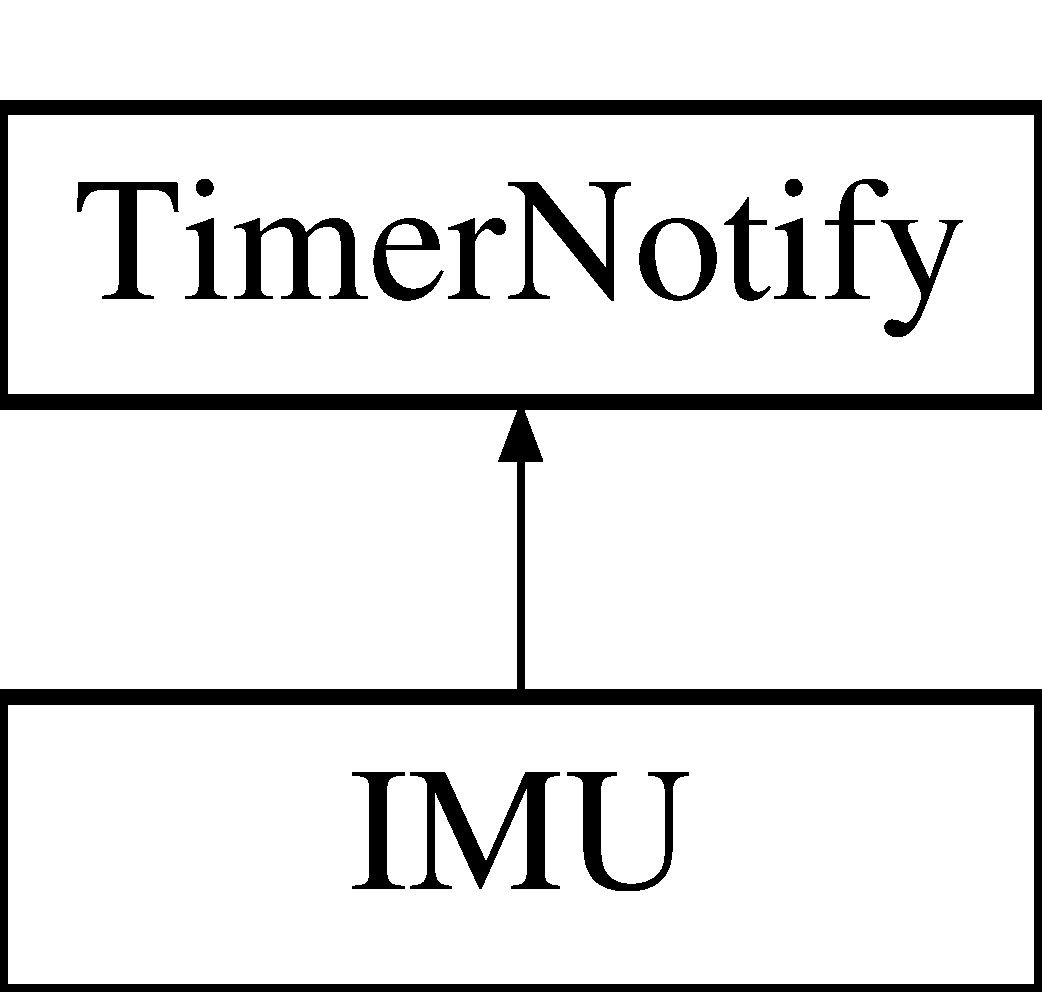
\includegraphics[height=2.000000cm]{class_timer_notify}
\end{center}
\end{figure}
\subsection*{Public Member Functions}
\begin{DoxyCompactItemize}
\item 
virtual void \hyperlink{class_timer_notify_a1b1d07d14c480883b6cda4d28b281978}{err} (uint8\_\-t id)=0
\item 
virtual void \hyperlink{class_timer_notify_a12081e2ac25688544b6f0c3de4bd412d}{ovf} (uint8\_\-t id)=0
\item 
virtual void \hyperlink{class_timer_notify_a2525b96a5e3ed4c4a039b296701f2b7e}{ccx} (uint8\_\-t id, uint8\_\-t idx)=0
\end{DoxyCompactItemize}


\subsection{Detailed Description}


Definition at line 5 of file TimerCntr.h.



\subsection{Member Function Documentation}
\hypertarget{class_timer_notify_a2525b96a5e3ed4c4a039b296701f2b7e}{
\index{TimerNotify@{TimerNotify}!ccx@{ccx}}
\index{ccx@{ccx}!TimerNotify@{TimerNotify}}
\subsubsection[{ccx}]{\setlength{\rightskip}{0pt plus 5cm}virtual void TimerNotify::ccx (
\begin{DoxyParamCaption}
\item[{uint8\_\-t}]{id, }
\item[{uint8\_\-t}]{idx}
\end{DoxyParamCaption}
)\hspace{0.3cm}{\ttfamily  \mbox{[}pure virtual\mbox{]}}}}
\label{class_timer_notify_a2525b96a5e3ed4c4a039b296701f2b7e}


Implemented in \hyperlink{class_i_m_u_ad2215ab5585c1f9512b91ef309dabf88}{IMU}.



Referenced by TimerCntr::ccx().

\hypertarget{class_timer_notify_a1b1d07d14c480883b6cda4d28b281978}{
\index{TimerNotify@{TimerNotify}!err@{err}}
\index{err@{err}!TimerNotify@{TimerNotify}}
\subsubsection[{err}]{\setlength{\rightskip}{0pt plus 5cm}virtual void TimerNotify::err (
\begin{DoxyParamCaption}
\item[{uint8\_\-t}]{id}
\end{DoxyParamCaption}
)\hspace{0.3cm}{\ttfamily  \mbox{[}pure virtual\mbox{]}}}}
\label{class_timer_notify_a1b1d07d14c480883b6cda4d28b281978}


Implemented in \hyperlink{class_i_m_u_ae56d268445b752f9720c814cb294ba40}{IMU}.



Referenced by TimerCntr::err().

\hypertarget{class_timer_notify_a12081e2ac25688544b6f0c3de4bd412d}{
\index{TimerNotify@{TimerNotify}!ovf@{ovf}}
\index{ovf@{ovf}!TimerNotify@{TimerNotify}}
\subsubsection[{ovf}]{\setlength{\rightskip}{0pt plus 5cm}virtual void TimerNotify::ovf (
\begin{DoxyParamCaption}
\item[{uint8\_\-t}]{id}
\end{DoxyParamCaption}
)\hspace{0.3cm}{\ttfamily  \mbox{[}pure virtual\mbox{]}}}}
\label{class_timer_notify_a12081e2ac25688544b6f0c3de4bd412d}


Implemented in \hyperlink{class_i_m_u_aefbd4e2f7f3928cf44c00a96d61c3546}{IMU}.



Referenced by TimerCntr::ovf().



The documentation for this class was generated from the following file:\begin{DoxyCompactItemize}
\item 
\hyperlink{_timer_cntr_8h}{TimerCntr.h}\end{DoxyCompactItemize}

\chapter{File Documentation}
\hypertarget{clksystem_8cpp}{
\subsection{clksystem.cpp File Reference}
\label{clksystem_8cpp}\index{clksystem.cpp@{clksystem.cpp}}
}
{\ttfamily \#include $<$avr/io.h$>$}\par
{\ttfamily \#include $<$util/delay.h$>$}\par
{\ttfamily \#include $<$avr/interrupt.h$>$}\par
{\ttfamily \#include $<$stdint.h$>$}\par
{\ttfamily \#include $<$stdbool.h$>$}\par
{\ttfamily \#include $<$stdlib.h$>$}\par
\subsubsection*{Defines}
\begin{DoxyCompactItemize}
\item 
\#define \hyperlink{clksystem_8cpp_a0a4fb62f9e69209c9c8c8e34ebb3df6f}{AVR\_\-ENTER\_\-CRITICAL\_\-REGION}()
\begin{DoxyCompactList}\small\item\em This macro will protect the following code from interrupts. \item\end{DoxyCompactList}\item 
\#define \hyperlink{clksystem_8cpp_a770b47b04eec57748be0826a3d23503b}{AVR\_\-LEAVE\_\-CRITICAL\_\-REGION}()~SREG = saved\_\-sreg;
\begin{DoxyCompactList}\small\item\em This macro must always be used in conjunction with AVR\_\-ENTER\_\-CRITICAL\_\-REGION so the interrupts are enabled again. \item\end{DoxyCompactList}\end{DoxyCompactItemize}
\subsubsection*{Functions}
\begin{DoxyCompactItemize}
\item 
void \hyperlink{clksystem_8cpp_aad4e162434c2cc7e0087bbc0ddfe266c}{CCPWrite} (volatile uint8\_\-t $\ast$address, uint8\_\-t value)
\begin{DoxyCompactList}\small\item\em CCP write helper function written in assembly. \item\end{DoxyCompactList}\item 
void \hyperlink{clksystem_8cpp_a098d30ebaad7a94505407605314930e5}{clksystem\_\-init} ()
\end{DoxyCompactItemize}


\subsubsection{Define Documentation}
\hypertarget{clksystem_8cpp_a0a4fb62f9e69209c9c8c8e34ebb3df6f}{
\index{clksystem.cpp@{clksystem.cpp}!AVR\_\-ENTER\_\-CRITICAL\_\-REGION@{AVR\_\-ENTER\_\-CRITICAL\_\-REGION}}
\index{AVR\_\-ENTER\_\-CRITICAL\_\-REGION@{AVR\_\-ENTER\_\-CRITICAL\_\-REGION}!clksystem.cpp@{clksystem.cpp}}
\paragraph[{AVR\_\-ENTER\_\-CRITICAL\_\-REGION}]{\setlength{\rightskip}{0pt plus 5cm}\#define AVR\_\-ENTER\_\-CRITICAL\_\-REGION(
\begin{DoxyParamCaption}
{}
\end{DoxyParamCaption}
)}\hfill}
\label{clksystem_8cpp_a0a4fb62f9e69209c9c8c8e34ebb3df6f}
{\bfseries Value:}
\begin{DoxyCode}
uint8\_t \textcolor{keyword}{volatile} saved\_sreg = SREG; \(\backslash\)
                                     cli();
\end{DoxyCode}


This macro will protect the following code from interrupts. 



Definition at line \hyperlink{clksystem_8cpp_source_l00010}{10} of file \hyperlink{clksystem_8cpp_source}{clksystem.cpp}.



Referenced by \hyperlink{clksystem_8cpp_source_l00026}{CCPWrite()}.

\hypertarget{clksystem_8cpp_a770b47b04eec57748be0826a3d23503b}{
\index{clksystem.cpp@{clksystem.cpp}!AVR\_\-LEAVE\_\-CRITICAL\_\-REGION@{AVR\_\-LEAVE\_\-CRITICAL\_\-REGION}}
\index{AVR\_\-LEAVE\_\-CRITICAL\_\-REGION@{AVR\_\-LEAVE\_\-CRITICAL\_\-REGION}!clksystem.cpp@{clksystem.cpp}}
\paragraph[{AVR\_\-LEAVE\_\-CRITICAL\_\-REGION}]{\setlength{\rightskip}{0pt plus 5cm}\#define AVR\_\-LEAVE\_\-CRITICAL\_\-REGION(
\begin{DoxyParamCaption}
{}
\end{DoxyParamCaption}
)~SREG = saved\_\-sreg;}\hfill}
\label{clksystem_8cpp_a770b47b04eec57748be0826a3d23503b}


This macro must always be used in conjunction with AVR\_\-ENTER\_\-CRITICAL\_\-REGION so the interrupts are enabled again. 



Definition at line \hyperlink{clksystem_8cpp_source_l00016}{16} of file \hyperlink{clksystem_8cpp_source}{clksystem.cpp}.



Referenced by \hyperlink{clksystem_8cpp_source_l00026}{CCPWrite()}.



\subsubsection{Function Documentation}
\hypertarget{clksystem_8cpp_aad4e162434c2cc7e0087bbc0ddfe266c}{
\index{clksystem.cpp@{clksystem.cpp}!CCPWrite@{CCPWrite}}
\index{CCPWrite@{CCPWrite}!clksystem.cpp@{clksystem.cpp}}
\paragraph[{CCPWrite}]{\setlength{\rightskip}{0pt plus 5cm}void CCPWrite (
\begin{DoxyParamCaption}
\item[{volatile uint8\_\-t $\ast$}]{address, }
\item[{uint8\_\-t}]{value}
\end{DoxyParamCaption}
)}\hfill}
\label{clksystem_8cpp_aad4e162434c2cc7e0087bbc0ddfe266c}


CCP write helper function written in assembly. 

This function is written in assembly because of the timecritial operation of writing to the registers.


\begin{DoxyParams}{Parameters}
{\em address} & A pointer to the address to write to. \\
\hline
{\em value} & The value to put in to the register. \\
\hline
\end{DoxyParams}


Definition at line \hyperlink{clksystem_8cpp_source_l00026}{26} of file \hyperlink{clksystem_8cpp_source}{clksystem.cpp}.



References \hyperlink{clksystem_8cpp_source_l00010}{AVR\_\-ENTER\_\-CRITICAL\_\-REGION}, and \hyperlink{clksystem_8cpp_source_l00016}{AVR\_\-LEAVE\_\-CRITICAL\_\-REGION}.


\begin{DoxyCode}
\{
    \hyperlink{clksystem_8cpp_a0a4fb62f9e69209c9c8c8e34ebb3df6f}{AVR_ENTER_CRITICAL_REGION}( );

    \textcolor{keyword}{volatile} uint8\_t * tmpAddr = address;

    \textcolor{keyword}{asm} \textcolor{keyword}{volatile}(
        \textcolor{stringliteral}{"movw r30,  %0"}       \textcolor{stringliteral}{"\(\backslash\)n\(\backslash\)t"}
        \textcolor{stringliteral}{"ldi  r16,  %2"}       \textcolor{stringliteral}{"\(\backslash\)n\(\backslash\)t"}
        \textcolor{stringliteral}{"out   %3, r16"}       \textcolor{stringliteral}{"\(\backslash\)n\(\backslash\)t"}
        \textcolor{stringliteral}{"st     Z,  %1"}       \textcolor{stringliteral}{"\(\backslash\)n\(\backslash\)t"}
        :
        : \textcolor{stringliteral}{"r"} (tmpAddr), \textcolor{stringliteral}{"r"} (value), \textcolor{stringliteral}{"M"} (0xD8), \textcolor{stringliteral}{"i"} (&CCP)
        : \textcolor{stringliteral}{"r16"}, \textcolor{stringliteral}{"r30"}, \textcolor{stringliteral}{"r31"}
    );

    \hyperlink{clksystem_8cpp_a770b47b04eec57748be0826a3d23503b}{AVR_LEAVE_CRITICAL_REGION}( );
\}
\end{DoxyCode}
\hypertarget{clksystem_8cpp_a098d30ebaad7a94505407605314930e5}{
\index{clksystem.cpp@{clksystem.cpp}!clksystem\_\-init@{clksystem\_\-init}}
\index{clksystem\_\-init@{clksystem\_\-init}!clksystem.cpp@{clksystem.cpp}}
\paragraph[{clksystem\_\-init}]{\setlength{\rightskip}{0pt plus 5cm}void clksystem\_\-init (
\begin{DoxyParamCaption}
{}
\end{DoxyParamCaption}
)}\hfill}
\label{clksystem_8cpp_a098d30ebaad7a94505407605314930e5}


Definition at line \hyperlink{clksystem_8cpp_source_l00058}{58} of file \hyperlink{clksystem_8cpp_source}{clksystem.cpp}.



Referenced by \hyperlink{_gyro_acc_8cpp_source_l00023}{init()}.


\begin{DoxyCode}
\{
    \textcolor{comment}{// This board does not have an external oscillator,}
    \textcolor{comment}{// so we need to use the internal oscillator.}
    \textcolor{comment}{// Enable the internal 32Mhz oscillator. Disables all the rest.}
    OSC.CTRL = OSC\_RC32MEN\_bm | OSC\_RC2MEN\_bm | OSC\_RC32KEN\_bm;

    \textcolor{comment}{//OSC.XOSCCTRL = 0; // we don't care, just set this to some value.}

    \textcolor{comment}{// Wait for the external oscilator. Don't wait forever though.}
    \textcolor{keywordtype}{int} maxWait = 100; \textcolor{comment}{// Wait 1 second}
    \textcolor{keywordflow}{while} (--maxWait && !(OSC.STATUS & (OSC\_RC32MRDY\_bm | OSC\_RC32KRDY\_bm | OSC\_R
      C2MRDY\_bm))) \{
        \_delay\_loop\_2(10);
    \}

    OSC.DFLLCTRL = 0;
    DFLLRC32M.CTRL = 0x1;
    DFLLRC2M.CTRL = 0x1;

    \textcolor{comment}{// If the external oscilator is running, then we can switch the PLL}
    \textcolor{comment}{// over to it and wait for the PLL to stabilize.}
    \textcolor{keywordflow}{if} (OSC.STATUS & ( OSC\_RC32MRDY\_bm | OSC\_RC2MRDY\_bm)) \{
        \textcolor{comment}{// Setup the PLL to use the internal 32Mhz oscillator and a}
        \textcolor{comment}{// factor of 4 to get a 128Mhz PLL Clock.}

        \textcolor{comment}{// Make sure this is disabled before we try and configure it.}
        OSC.CTRL &= ~OSC\_PLLEN\_bm;

        OSC.PLLCTRL = OSC\_PLLSRC\_RC32M\_gc | (16 << OSC\_PLLFAC\_gp);

        OSC.CTRL |= OSC\_PLLEN\_bm;

        \textcolor{comment}{//OSC.CTRL = CLK\_PSADIV\_16\_gc;}
        \textcolor{comment}{// Wait for OSC.STATUS to indicate that PLL is ready..}
        \textcolor{keywordflow}{while} (!(OSC.STATUS & OSC\_PLLRDY\_bm)) \{
        \}

        \textcolor{comment}{// Okay, the PLL is up on the new clock. Set the prescalers then}
        \textcolor{comment}{// switch over to the PLL.}

        CCP = CCP\_IOREG\_gc;
        CLK.PSCTRL = CLK\_PSADIV\_1\_gc | CLK\_PSBCDIV\_2\_2\_gc;
        \textcolor{comment}{//CLK.PSCTRL = CLK\_PSADIV\_1\_gc | CLK\_PSBCDIV\_1\_1\_gc;}

        \textcolor{comment}{// When all is done, make the PLL be the clock source for the system.}
        CCP = CCP\_IOREG\_gc;
        CLK.CTRL = CLK\_SCLKSEL\_PLL\_gc;
        \textcolor{comment}{//CLK.CTRL = CLK\_SCLKSEL\_RC32M\_gc;}
        \textcolor{comment}{//CLK.CTRL = CLK\_SCLKSEL\_RC2M\_gc;}
    \}
\}
\end{DoxyCode}

\hypertarget{clksystem_8h}{
\section{clksystem.h File Reference}
\label{clksystem_8h}\index{clksystem.h@{clksystem.h}}
}
\subsection*{Functions}
\begin{DoxyCompactItemize}
\item 
int \hyperlink{clksystem_8h_a8e83774f95a168320aacc0f85718b483}{clksystem\_\-init} ()
\end{DoxyCompactItemize}


\subsection{Function Documentation}
\hypertarget{clksystem_8h_a8e83774f95a168320aacc0f85718b483}{
\index{clksystem.h@{clksystem.h}!clksystem\_\-init@{clksystem\_\-init}}
\index{clksystem\_\-init@{clksystem\_\-init}!clksystem.h@{clksystem.h}}
\subsubsection[{clksystem\_\-init}]{\setlength{\rightskip}{0pt plus 5cm}int clksystem\_\-init (
\begin{DoxyParamCaption}
{}
\end{DoxyParamCaption}
)}}
\label{clksystem_8h_a8e83774f95a168320aacc0f85718b483}


Definition at line 58 of file clksystem.cpp.



Referenced by init().


\begin{DoxyCode}
{
    // This board does not have an external oscillator,
    // so we need to use the internal oscillator.
    // Enable the internal 32Mhz oscillator. Disables all the rest.
    OSC.CTRL = OSC_RC32MEN_bm | OSC_RC2MEN_bm | OSC_RC32KEN_bm;

    //OSC.XOSCCTRL = 0; // we don't care, just set this to some value.

    // Wait for the external oscilator. Don't wait forever though.
    int maxWait = 100; // Wait 1 second
    while (--maxWait && !(OSC.STATUS & (OSC_RC32MRDY_bm | OSC_RC32KRDY_bm | OSC_R
      C2MRDY_bm))) {
        _delay_loop_2(10);
    }

    OSC.DFLLCTRL = 0;
    DFLLRC32M.CTRL = 0x1;
    DFLLRC2M.CTRL = 0x1;

    // If the external oscilator is running, then we can switch the PLL
    // over to it and wait for the PLL to stabilize.
    if (OSC.STATUS & ( OSC_RC32MRDY_bm | OSC_RC2MRDY_bm)) {
        // Setup the PLL to use the internal 32Mhz oscillator and a
        // factor of 4 to get a 128Mhz PLL Clock.

        // Make sure this is disabled before we try and configure it.
        OSC.CTRL &= ~OSC_PLLEN_bm;

        OSC.PLLCTRL = OSC_PLLSRC_RC32M_gc | (16 << OSC_PLLFAC_gp);

        OSC.CTRL |= OSC_PLLEN_bm;

        //OSC.CTRL = CLK_PSADIV_16_gc;
        // Wait for OSC.STATUS to indicate that PLL is ready..
        while (!(OSC.STATUS & OSC_PLLRDY_bm)) {
        }

        // Okay, the PLL is up on the new clock. Set the prescalers then
        // switch over to the PLL.

        CCP = CCP_IOREG_gc;
        CLK.PSCTRL = CLK_PSADIV_1_gc | CLK_PSBCDIV_2_2_gc;
        //CLK.PSCTRL = CLK_PSADIV_1_gc | CLK_PSBCDIV_1_1_gc;

        // When all is done, make the PLL be the clock source for the system.
        CCP = CCP_IOREG_gc;
        CLK.CTRL = CLK_SCLKSEL_PLL_gc;
        //CLK.CTRL = CLK_SCLKSEL_RC32M_gc;
        //CLK.CTRL = CLK_SCLKSEL_RC2M_gc;
    }
}
\end{DoxyCode}

\hypertarget{_cmd_processor_8cpp}{
\subsection{CmdProcessor.cpp File Reference}
\label{_cmd_processor_8cpp}\index{CmdProcessor.cpp@{CmdProcessor.cpp}}
}
{\ttfamily \#include $<$stdlib.h$>$}\par
{\ttfamily \#include $<$string.h$>$}\par
{\ttfamily \#include \char`\"{}CmdProcessor.h\char`\"{}}\par

\hypertarget{_cmd_processor_8h}{
\section{CmdProcessor.h File Reference}
\label{_cmd_processor_8h}\index{CmdProcessor.h@{CmdProcessor.h}}
}
{\ttfamily \#include $<$avr/io.h$>$}\par
{\ttfamily \#include \char`\"{}HardwareSerial.h\char`\"{}}\par
\subsection*{Classes}
\begin{DoxyCompactItemize}
\item 
class \hyperlink{class_cmd_processor}{CmdProcessor}
\end{DoxyCompactItemize}

\hypertarget{cpp__hacks_8cpp}{
\section{cpp\_\-hacks.cpp File Reference}
\label{cpp__hacks_8cpp}\index{cpp\_\-hacks.cpp@{cpp\_\-hacks.cpp}}
}
{\ttfamily \#include \char`\"{}cpp\_\-hacks.h\char`\"{}}\par
\subsection*{Functions}
\begin{DoxyCompactItemize}
\item 
int \hyperlink{cpp__hacks_8cpp_ad9a42607fb7932f44ba914ac49972e62}{\_\-\_\-cxa\_\-guard\_\-acquire} (\_\-\_\-guard $\ast$g)
\item 
void \hyperlink{cpp__hacks_8cpp_adef76ddddaddf969efa3bfad968fd430}{\_\-\_\-cxa\_\-guard\_\-release} (\_\-\_\-guard $\ast$g)
\item 
void \hyperlink{cpp__hacks_8cpp_a357afb2dc20a652447f3a529dbda60e4}{\_\-\_\-cxa\_\-guard\_\-abort} (\_\-\_\-guard $\ast$)
\item 
void \hyperlink{cpp__hacks_8cpp_a4464d4205cf92370b8d5077d93bc48a6}{\_\-\_\-cxa\_\-pure\_\-virtual} (void)
\end{DoxyCompactItemize}


\subsection{Function Documentation}
\hypertarget{cpp__hacks_8cpp_a357afb2dc20a652447f3a529dbda60e4}{
\index{cpp\_\-hacks.cpp@{cpp\_\-hacks.cpp}!\_\-\_\-cxa\_\-guard\_\-abort@{\_\-\_\-cxa\_\-guard\_\-abort}}
\index{\_\-\_\-cxa\_\-guard\_\-abort@{\_\-\_\-cxa\_\-guard\_\-abort}!cpp_hacks.cpp@{cpp\_\-hacks.cpp}}
\subsubsection[{\_\-\_\-cxa\_\-guard\_\-abort}]{\setlength{\rightskip}{0pt plus 5cm}void \_\-\_\-cxa\_\-guard\_\-abort (
\begin{DoxyParamCaption}
\item[{\_\-\_\-guard $\ast$}]{}
\end{DoxyParamCaption}
)}}
\label{cpp__hacks_8cpp_a357afb2dc20a652447f3a529dbda60e4}


Definition at line 5 of file cpp\_\-hacks.cpp.


\begin{DoxyCode}
{}; 
\end{DoxyCode}
\hypertarget{cpp__hacks_8cpp_ad9a42607fb7932f44ba914ac49972e62}{
\index{cpp\_\-hacks.cpp@{cpp\_\-hacks.cpp}!\_\-\_\-cxa\_\-guard\_\-acquire@{\_\-\_\-cxa\_\-guard\_\-acquire}}
\index{\_\-\_\-cxa\_\-guard\_\-acquire@{\_\-\_\-cxa\_\-guard\_\-acquire}!cpp_hacks.cpp@{cpp\_\-hacks.cpp}}
\subsubsection[{\_\-\_\-cxa\_\-guard\_\-acquire}]{\setlength{\rightskip}{0pt plus 5cm}int \_\-\_\-cxa\_\-guard\_\-acquire (
\begin{DoxyParamCaption}
\item[{\_\-\_\-guard $\ast$}]{g}
\end{DoxyParamCaption}
)}}
\label{cpp__hacks_8cpp_ad9a42607fb7932f44ba914ac49972e62}


Definition at line 3 of file cpp\_\-hacks.cpp.


\begin{DoxyCode}
{return !*(char *)(g);}; 
\end{DoxyCode}
\hypertarget{cpp__hacks_8cpp_adef76ddddaddf969efa3bfad968fd430}{
\index{cpp\_\-hacks.cpp@{cpp\_\-hacks.cpp}!\_\-\_\-cxa\_\-guard\_\-release@{\_\-\_\-cxa\_\-guard\_\-release}}
\index{\_\-\_\-cxa\_\-guard\_\-release@{\_\-\_\-cxa\_\-guard\_\-release}!cpp_hacks.cpp@{cpp\_\-hacks.cpp}}
\subsubsection[{\_\-\_\-cxa\_\-guard\_\-release}]{\setlength{\rightskip}{0pt plus 5cm}void \_\-\_\-cxa\_\-guard\_\-release (
\begin{DoxyParamCaption}
\item[{\_\-\_\-guard $\ast$}]{g}
\end{DoxyParamCaption}
)}}
\label{cpp__hacks_8cpp_adef76ddddaddf969efa3bfad968fd430}


Definition at line 4 of file cpp\_\-hacks.cpp.


\begin{DoxyCode}
{*(char *)g = 1;}; 
\end{DoxyCode}
\hypertarget{cpp__hacks_8cpp_a4464d4205cf92370b8d5077d93bc48a6}{
\index{cpp\_\-hacks.cpp@{cpp\_\-hacks.cpp}!\_\-\_\-cxa\_\-pure\_\-virtual@{\_\-\_\-cxa\_\-pure\_\-virtual}}
\index{\_\-\_\-cxa\_\-pure\_\-virtual@{\_\-\_\-cxa\_\-pure\_\-virtual}!cpp_hacks.cpp@{cpp\_\-hacks.cpp}}
\subsubsection[{\_\-\_\-cxa\_\-pure\_\-virtual}]{\setlength{\rightskip}{0pt plus 5cm}void \_\-\_\-cxa\_\-pure\_\-virtual (
\begin{DoxyParamCaption}
\item[{void}]{}
\end{DoxyParamCaption}
)}}
\label{cpp__hacks_8cpp_a4464d4205cf92370b8d5077d93bc48a6}


Definition at line 7 of file cpp\_\-hacks.cpp.


\begin{DoxyCode}
{}; 
\end{DoxyCode}

\hypertarget{cpp__hacks_8h}{
\section{cpp\_\-hacks.h File Reference}
\label{cpp__hacks_8h}\index{cpp\_\-hacks.h@{cpp\_\-hacks.h}}
}
\subsection*{Functions}
\begin{DoxyCompactItemize}
\item 
\_\-\_\-extension\_\-\_\- typedef int \_\-\_\-guard \hyperlink{cpp__hacks_8h_aa5aa60072f4063655d5283b6d7b7ab44}{\_\-\_\-attribute\_\-\_\-} ((mode(\_\-\_\-DI\_\-\_\-)))
\item 
int \hyperlink{cpp__hacks_8h_a239ddd7f6e7ee1b05b59b2e56d8afb40}{\_\-\_\-cxa\_\-guard\_\-acquire} (\_\-\_\-guard $\ast$)
\item 
void \hyperlink{cpp__hacks_8h_aab72c37f0b3e6fc38d293bd4f8dd61ed}{\_\-\_\-cxa\_\-guard\_\-release} (\_\-\_\-guard $\ast$)
\item 
void \hyperlink{cpp__hacks_8h_a357afb2dc20a652447f3a529dbda60e4}{\_\-\_\-cxa\_\-guard\_\-abort} (\_\-\_\-guard $\ast$)
\item 
void \hyperlink{cpp__hacks_8h_a4464d4205cf92370b8d5077d93bc48a6}{\_\-\_\-cxa\_\-pure\_\-virtual} (void)
\end{DoxyCompactItemize}


\subsection{Function Documentation}
\hypertarget{cpp__hacks_8h_aa5aa60072f4063655d5283b6d7b7ab44}{
\index{cpp\_\-hacks.h@{cpp\_\-hacks.h}!\_\-\_\-attribute\_\-\_\-@{\_\-\_\-attribute\_\-\_\-}}
\index{\_\-\_\-attribute\_\-\_\-@{\_\-\_\-attribute\_\-\_\-}!cpp_hacks.h@{cpp\_\-hacks.h}}
\subsubsection[{\_\-\_\-attribute\_\-\_\-}]{\setlength{\rightskip}{0pt plus 5cm}\_\-\_\-extension\_\-\_\- typedef int \_\-\_\-guard \_\-\_\-attribute\_\-\_\- (
\begin{DoxyParamCaption}
\item[{(mode(\_\-\_\-DI\_\-\_\-))}]{}
\end{DoxyParamCaption}
)}}
\label{cpp__hacks_8h_aa5aa60072f4063655d5283b6d7b7ab44}
\hypertarget{cpp__hacks_8h_a357afb2dc20a652447f3a529dbda60e4}{
\index{cpp\_\-hacks.h@{cpp\_\-hacks.h}!\_\-\_\-cxa\_\-guard\_\-abort@{\_\-\_\-cxa\_\-guard\_\-abort}}
\index{\_\-\_\-cxa\_\-guard\_\-abort@{\_\-\_\-cxa\_\-guard\_\-abort}!cpp_hacks.h@{cpp\_\-hacks.h}}
\subsubsection[{\_\-\_\-cxa\_\-guard\_\-abort}]{\setlength{\rightskip}{0pt plus 5cm}void \_\-\_\-cxa\_\-guard\_\-abort (
\begin{DoxyParamCaption}
\item[{\_\-\_\-guard $\ast$}]{}
\end{DoxyParamCaption}
)}}
\label{cpp__hacks_8h_a357afb2dc20a652447f3a529dbda60e4}


Definition at line 5 of file cpp\_\-hacks.cpp.


\begin{DoxyCode}
{}; 
\end{DoxyCode}
\hypertarget{cpp__hacks_8h_a239ddd7f6e7ee1b05b59b2e56d8afb40}{
\index{cpp\_\-hacks.h@{cpp\_\-hacks.h}!\_\-\_\-cxa\_\-guard\_\-acquire@{\_\-\_\-cxa\_\-guard\_\-acquire}}
\index{\_\-\_\-cxa\_\-guard\_\-acquire@{\_\-\_\-cxa\_\-guard\_\-acquire}!cpp_hacks.h@{cpp\_\-hacks.h}}
\subsubsection[{\_\-\_\-cxa\_\-guard\_\-acquire}]{\setlength{\rightskip}{0pt plus 5cm}int \_\-\_\-cxa\_\-guard\_\-acquire (
\begin{DoxyParamCaption}
\item[{\_\-\_\-guard $\ast$}]{}
\end{DoxyParamCaption}
)}}
\label{cpp__hacks_8h_a239ddd7f6e7ee1b05b59b2e56d8afb40}


Definition at line 3 of file cpp\_\-hacks.cpp.


\begin{DoxyCode}
{return !*(char *)(g);}; 
\end{DoxyCode}
\hypertarget{cpp__hacks_8h_aab72c37f0b3e6fc38d293bd4f8dd61ed}{
\index{cpp\_\-hacks.h@{cpp\_\-hacks.h}!\_\-\_\-cxa\_\-guard\_\-release@{\_\-\_\-cxa\_\-guard\_\-release}}
\index{\_\-\_\-cxa\_\-guard\_\-release@{\_\-\_\-cxa\_\-guard\_\-release}!cpp_hacks.h@{cpp\_\-hacks.h}}
\subsubsection[{\_\-\_\-cxa\_\-guard\_\-release}]{\setlength{\rightskip}{0pt plus 5cm}void \_\-\_\-cxa\_\-guard\_\-release (
\begin{DoxyParamCaption}
\item[{\_\-\_\-guard $\ast$}]{}
\end{DoxyParamCaption}
)}}
\label{cpp__hacks_8h_aab72c37f0b3e6fc38d293bd4f8dd61ed}


Definition at line 4 of file cpp\_\-hacks.cpp.


\begin{DoxyCode}
{*(char *)g = 1;}; 
\end{DoxyCode}
\hypertarget{cpp__hacks_8h_a4464d4205cf92370b8d5077d93bc48a6}{
\index{cpp\_\-hacks.h@{cpp\_\-hacks.h}!\_\-\_\-cxa\_\-pure\_\-virtual@{\_\-\_\-cxa\_\-pure\_\-virtual}}
\index{\_\-\_\-cxa\_\-pure\_\-virtual@{\_\-\_\-cxa\_\-pure\_\-virtual}!cpp_hacks.h@{cpp\_\-hacks.h}}
\subsubsection[{\_\-\_\-cxa\_\-pure\_\-virtual}]{\setlength{\rightskip}{0pt plus 5cm}void \_\-\_\-cxa\_\-pure\_\-virtual (
\begin{DoxyParamCaption}
\item[{void}]{}
\end{DoxyParamCaption}
)}}
\label{cpp__hacks_8h_a4464d4205cf92370b8d5077d93bc48a6}


Definition at line 7 of file cpp\_\-hacks.cpp.


\begin{DoxyCode}
{}; 
\end{DoxyCode}

\hypertarget{_documentation_8html}{
\section{Documentation.html File Reference}
\label{_documentation_8html}\index{Documentation.html@{Documentation.html}}
}

\hypertarget{fifo_8cpp}{
\section{fifo.cpp File Reference}
\label{fifo_8cpp}\index{fifo.cpp@{fifo.cpp}}
}
{\ttfamily \#include $<$stdio.h$>$}\par
{\ttfamily \#include $<$string.h$>$}\par
{\ttfamily \#include $<$math.h$>$}\par
{\ttfamily \#include \char`\"{}NewDel.h\char`\"{}}\par
{\ttfamily \#include \char`\"{}fifo.h\char`\"{}}\par
\subsection*{Functions}
\begin{DoxyCompactItemize}
\item 
void \hyperlink{fifo_8cpp_a9a948b7bfe866c00cfb8e3a5fea891ad}{FifoTest} (\hyperlink{class_hardware_serial}{HardwareSerial} \&ds)
\end{DoxyCompactItemize}


\subsection{Function Documentation}
\hypertarget{fifo_8cpp_a9a948b7bfe866c00cfb8e3a5fea891ad}{
\index{fifo.cpp@{fifo.cpp}!FifoTest@{FifoTest}}
\index{FifoTest@{FifoTest}!fifo.cpp@{fifo.cpp}}
\subsubsection[{FifoTest}]{\setlength{\rightskip}{0pt plus 5cm}void FifoTest (
\begin{DoxyParamCaption}
\item[{{\bf HardwareSerial} \&}]{ds}
\end{DoxyParamCaption}
)}}
\label{fifo_8cpp_a9a948b7bfe866c00cfb8e3a5fea891ad}
Test function to validate that the fifo works as expected. It is always a good idea to validate your data structures. Languages like Python or Perl have such validation built in, while C++ does not. This function can be used in a special build to run through some test cases and make sure that the fifo behaves as we exect, especially in the edge cases, such as when it gets full, wraps around, etc. 

Definition at line 110 of file fifo.cpp.



References buffer, Fifo::clear(), Fifo::count(), Fifo::pop(), Print::print(), and Fifo::push().


\begin{DoxyCode}
{
    Fifo f1(20);
    Fifo::FifoType x;
    char    buffer[128];
    
    for (x=1;x<25;x++) {
        f1.push(&x);
        sprintf(buffer,"Fifo push %d count %d\n",x,f1.count());
        ds.print(buffer);
    }
    f1.clear();
    sprintf(buffer,"Fifo count %d\n",f1.count());
    ds.print(buffer);
    
    for (x=0;x<10;x++) {
        f1.push(&x);
    }
    sprintf(buffer,"Fifo count %d. Expected 10\n",f1.count());
    ds.print(buffer);
    
    Fifo::FifoType y;
    for (x=1;x<15;x++) {
        f1.pop(&y);
        sprintf(buffer,"Fifo pop %d count %d\n",y,f1.count());
        ds.print(buffer);
    }
}
\end{DoxyCode}

\hypertarget{fifo_8h}{
\subsection{fifo.h File Reference}
\label{fifo_8h}\index{fifo.h@{fifo.h}}
}
{\ttfamily \#include $<$inttypes.h$>$}\par
{\ttfamily \#include \char`\"{}HardwareSerial.h\char`\"{}}\par
\subsubsection*{Classes}
\begin{DoxyCompactItemize}
\item 
class \hyperlink{class_fifo}{Fifo}
\begin{DoxyCompactList}\small\item\em \hyperlink{class_fifo}{Fifo} Class for unsigned 8 bit values. \item\end{DoxyCompactList}\end{DoxyCompactItemize}
\subsubsection*{Functions}
\begin{DoxyCompactItemize}
\item 
void \hyperlink{fifo_8h_a9a948b7bfe866c00cfb8e3a5fea891ad}{FifoTest} (\hyperlink{class_hardware_serial}{HardwareSerial} \&ds)
\end{DoxyCompactItemize}


\subsubsection{Function Documentation}
\hypertarget{fifo_8h_a9a948b7bfe866c00cfb8e3a5fea891ad}{
\index{fifo.h@{fifo.h}!FifoTest@{FifoTest}}
\index{FifoTest@{FifoTest}!fifo.h@{fifo.h}}
\paragraph[{FifoTest}]{\setlength{\rightskip}{0pt plus 5cm}void FifoTest (
\begin{DoxyParamCaption}
\item[{{\bf HardwareSerial} \&}]{ds}
\end{DoxyParamCaption}
)}\hfill}
\label{fifo_8h_a9a948b7bfe866c00cfb8e3a5fea891ad}
Test function to validate that the fifo works as expected. It is always a good idea to validate your data structures. Languages like Python or Perl have such validation built in, while C++ does not. This function can be used in a special build to run through some test cases and make sure that the fifo behaves as we exect, especially in the edge cases, such as when it gets full, wraps around, etc. 

Definition at line \hyperlink{fifo_8cpp_source_l00110}{110} of file \hyperlink{fifo_8cpp_source}{fifo.cpp}.



References \hyperlink{_i_m_u_8cpp_source_l00016}{buffer}, \hyperlink{fifo_8cpp_source_l00022}{Fifo::clear()}, \hyperlink{fifo_8cpp_source_l00050}{Fifo::count()}, \hyperlink{fifo_8cpp_source_l00092}{Fifo::pop()}, \hyperlink{_print_8cpp_source_l00045}{Print::print()}, and \hyperlink{fifo_8cpp_source_l00074}{Fifo::push()}.


\begin{DoxyCode}
\{
    \hyperlink{class_fifo}{Fifo} f1(20);
    \hyperlink{class_fifo_abc2a9e471beb538424db9e33955ec5f7}{Fifo::FifoType} x;
    \textcolor{keywordtype}{char}    \hyperlink{_i_m_u_8cpp_a38e7c3f1ce348a3ed20459d277245263}{buffer}[128];
    
    \textcolor{keywordflow}{for} (x=1;x<25;x++) \{
        f1.push(&x);
        sprintf(buffer,\textcolor{stringliteral}{"Fifo push %d count %d\(\backslash\)n"},x,f1.count());
        ds.\hyperlink{class_print_aa7b0a6dc63e3d27effd8459e3d443b83}{print}(buffer);
    \}
    f1.clear();
    sprintf(buffer,\textcolor{stringliteral}{"Fifo count %d\(\backslash\)n"},f1.count());
    ds.\hyperlink{class_print_aa7b0a6dc63e3d27effd8459e3d443b83}{print}(buffer);
    
    \textcolor{keywordflow}{for} (x=0;x<10;x++) \{
        f1.push(&x);
    \}
    sprintf(buffer,\textcolor{stringliteral}{"Fifo count %d. Expected 10\(\backslash\)n"},f1.count());
    ds.\hyperlink{class_print_aa7b0a6dc63e3d27effd8459e3d443b83}{print}(buffer);
    
    \hyperlink{class_fifo_abc2a9e471beb538424db9e33955ec5f7}{Fifo::FifoType} y;
    \textcolor{keywordflow}{for} (x=1;x<15;x++) \{
        f1.pop(&y);
        sprintf(buffer,\textcolor{stringliteral}{"Fifo pop %d count %d\(\backslash\)n"},y,f1.count());
        ds.\hyperlink{class_print_aa7b0a6dc63e3d27effd8459e3d443b83}{print}(buffer);
    \}
\}
\end{DoxyCode}

\hypertarget{_gyro_acc_8cpp}{
\section{GyroAcc.cpp File Reference}
\label{_gyro_acc_8cpp}\index{GyroAcc.cpp@{GyroAcc.cpp}}
}
{\ttfamily \#include $<$avr/io.h$>$}\par
{\ttfamily \#include $<$avr/interrupt.h$>$}\par
{\ttfamily \#include $<$util/delay.h$>$}\par
{\ttfamily \#include $<$string.h$>$}\par
{\ttfamily \#include \char`\"{}NewDel.h\char`\"{}}\par
{\ttfamily \#include \char`\"{}clksystem.h\char`\"{}}\par
{\ttfamily \#include \char`\"{}time.h\char`\"{}}\par
{\ttfamily \#include \char`\"{}HardwareSerial.h\char`\"{}}\par
{\ttfamily \#include \char`\"{}GyroCmdProcessor.h\char`\"{}}\par
{\ttfamily \#include \char`\"{}I2C\_\-Master.h\char`\"{}}\par
{\ttfamily \#include \char`\"{}IMU.h\char`\"{}}\par
{\ttfamily \#include \char`\"{}IMUManager.h\char`\"{}}\par
{\ttfamily \#include \char`\"{}TimerCntr.h\char`\"{}}\par
{\ttfamily \#include \char`\"{}Port.h\char`\"{}}\par
{\ttfamily \#include \char`\"{}MyDriver.h\char`\"{}}\par
{\ttfamily \#include \char`\"{}Revision.h\char`\"{}}\par
\subsection*{Functions}
\begin{DoxyCompactItemize}
\item 
void \hyperlink{_gyro_acc_8cpp_a896a4c37c6ecf8868ef0dc758e5a598c}{timer\_\-init} ()
\begin{DoxyCompactList}\small\item\em Declared in TimerCore.cpp. \item\end{DoxyCompactList}\item 
void \hyperlink{_gyro_acc_8cpp_a02fd73d861ef2e4aabb38c0c9ff82947}{init} ()
\item 
void \hyperlink{_gyro_acc_8cpp_a04545dccf7a169ce181b81c5376c9ec7}{processCmd} (\hyperlink{class_cmd_processor}{CmdProcessor} \&cmdproc)
\item 
int \hyperlink{_gyro_acc_8cpp_ae66f6b31b5ad750f1fe042a706a4e3d4}{main} ()
\end{DoxyCompactItemize}
\subsection*{Variables}
\begin{DoxyCompactItemize}
\item 
\hyperlink{class_hardware_serial}{HardwareSerial} $\ast$ \hyperlink{_gyro_acc_8cpp_a953e918236b1fd18b8f07bad1217ecbe}{pdbgserial} = 0
\item 
DebugPort $\ast$ \hyperlink{_gyro_acc_8cpp_ab6b6625a30d84db3519866cb8c32dd39}{pdbgport} = 0
\end{DoxyCompactItemize}


\subsection{Function Documentation}
\hypertarget{_gyro_acc_8cpp_a02fd73d861ef2e4aabb38c0c9ff82947}{
\index{GyroAcc.cpp@{GyroAcc.cpp}!init@{init}}
\index{init@{init}!GyroAcc.cpp@{GyroAcc.cpp}}
\subsubsection[{init}]{\setlength{\rightskip}{0pt plus 5cm}void init (
\begin{DoxyParamCaption}
{}
\end{DoxyParamCaption}
)}}
\label{_gyro_acc_8cpp_a02fd73d861ef2e4aabb38c0c9ff82947}


Definition at line 23 of file GyroAcc.cpp.



References clksystem\_\-init(), and timer\_\-init().



Referenced by main().


\begin{DoxyCode}
            {

    clksystem_init();
    timer_init();
}
\end{DoxyCode}
\hypertarget{_gyro_acc_8cpp_ae66f6b31b5ad750f1fe042a706a4e3d4}{
\index{GyroAcc.cpp@{GyroAcc.cpp}!main@{main}}
\index{main@{main}!GyroAcc.cpp@{GyroAcc.cpp}}
\subsubsection[{main}]{\setlength{\rightskip}{0pt plus 5cm}int main (
\begin{DoxyParamCaption}
{}
\end{DoxyParamCaption}
)}}
\label{_gyro_acc_8cpp_ae66f6b31b5ad750f1fe042a706a4e3d4}


Create timers for each of the \hyperlink{class_i_m_u}{IMU} Masters. I use the TCx1 timers which are less capable, but it hardly matters as these are just setting a timer callback.

Give the rate a default value. Start low

This bit just toggles the light 



Definition at line 34 of file GyroAcc.cpp.



References HardwareSerial::begin(), buffer, HardwareSerial::enable(), init(), pdbgport, Print::print(), IMU::SetDebugPort(), and IMU::SetDebugPort2().


\begin{DoxyCode}
{
    char    buffer[100];
    init();

    PMIC.CTRL |= PMIC_HILVLEN_bm | PMIC_LOLVLEN_bm | PMIC_MEDLVLEN_bm;
    sei();
    
#ifdef USE_DEBUGPORT_2
    DebugPort dbgPort2(&PORTE);
    dbgPort2.PinMask(0xF0,5);
    dbgPort2.SetState(0);
#endif
    
    HardwareSerial dbgserial(&USARTF1, &PORTF, PIN6_bm, PIN7_bm);
    dbgserial.begin(115200);
    pdbgserial = &dbgserial;
    pdbgserial->enable(false);

    // Instantiate a commad processor.
    // Specify the USART, PORT, rxPin and txPin and the baud rate.
    HardwareSerial cmdSerial(&USARTD0, &PORTD, PIN2_bm, PIN3_bm);
    cmdSerial.begin(115200);
    //cmdSerial.begin(285000);
    //cmdSerial.begin(921600);
    
    CCP = CCP_IOREG_gc;
    MCU.MCUCR = MCU_JTAGD_bm;
    DebugPort dbgPort(&PORTB);
    dbgPort.PinMask(0xF0,4);
    dbgPort.SetState(0xf);
    dbgPort.SetState(0);
    pdbgport = &dbgPort;

    I2C_Master  *pMaster[4];
    I2C_Master hand(&TWIC);
    I2C_Master single(&TWID);
    I2C_Master pair1(&TWIE);
    I2C_Master pair2(&TWIF);

    pMaster[0] = &hand;
    pMaster[1] = &single; // Pinkie
    pMaster[2] = &pair1;  // Ring + Middle
    pMaster[3] = &pair2;  // Index + Thumb
    
    for (int x=0;x<4;x++) {
        if (pMaster[x]) {
            pMaster[x]->begin(400e3);
        }
    }

    // Give the hardware time to stabilize..
    _delay_ms(1000);
    
    // When constructed without a list of ID's, the IMU will query known
    // ID's 0xD0 and 0xD2 for the Gyro, and then 0x30 and 0x32 respectively
    // for the ACC.
    IMU     hand_imu(&hand);    
    IMU     single_imu(&single);
    IMU     pair1_imu(&pair1);  
    IMU     pair2_imu(&pair2);  

    // These all share the debug port, so they must operate
    // in sequence. If I went back to a parallel operation, then
    // this would have to change.
    hand_imu.SetDebugPort(&dbgPort);

    single_imu.SetDebugPort(&dbgPort);

    pair1_imu.SetDebugPort(&dbgPort);

    pair2_imu.SetDebugPort(&dbgPort);

#ifdef USE_DEBUGPORT_2
    hand_imu.SetDebugPort2(&dbgPort2);
    single_imu.SetDebugPort2(&dbgPort2);
    pair1_imu.SetDebugPort2(&dbgPort2);
    pair2_imu.SetDebugPort2(&dbgPort2);
#endif
    
    TimerCntr   tcA(&TCC1);
    
    IMUManager imumgr(&cmdSerial);
    imumgr.SetBlueLed(&PORTJ, PIN7_bm);
    imumgr.LedOff();
    imumgr.SetTimer(&tcA);
    imumgr.AddIMU(&hand_imu);
    imumgr.AddIMU(&single_imu);
    imumgr.AddIMU(&pair1_imu);
    imumgr.AddIMU(&pair2_imu);
    imumgr.SampleRate(10); 
    
    GyroCmdProcessor cmdproc(&cmdSerial,&pMaster[0],&imumgr);

    sprintf(buffer,"Welcome to Gyro Glove.\nRev %d.%d.%d Date: %02d/%02d/%04d Bui
      lt at: %02d:%02d\n",
        RevMajor, RevMinor, RevInc,
        DateMonth, DateDay, DateYear,
        TimeHour, TimeMin
        );
    cmdSerial.print(buffer);
    
    TimerCntr mdtc(&TCD0);
    MyDriver md;
    md.SetTimer(&mdtc);
    
    cmdSerial.print("Starting endless loop\n");
    
    while(1) {
        cmdproc.Loop();        
        imumgr.Loop();
    }

    return 0;
}
\end{DoxyCode}
\hypertarget{_gyro_acc_8cpp_a04545dccf7a169ce181b81c5376c9ec7}{
\index{GyroAcc.cpp@{GyroAcc.cpp}!processCmd@{processCmd}}
\index{processCmd@{processCmd}!GyroAcc.cpp@{GyroAcc.cpp}}
\subsubsection[{processCmd}]{\setlength{\rightskip}{0pt plus 5cm}void processCmd (
\begin{DoxyParamCaption}
\item[{{\bf CmdProcessor} \&}]{cmdproc}
\end{DoxyParamCaption}
)}}
\label{_gyro_acc_8cpp_a04545dccf7a169ce181b81c5376c9ec7}
\hypertarget{_gyro_acc_8cpp_a896a4c37c6ecf8868ef0dc758e5a598c}{
\index{GyroAcc.cpp@{GyroAcc.cpp}!timer\_\-init@{timer\_\-init}}
\index{timer\_\-init@{timer\_\-init}!GyroAcc.cpp@{GyroAcc.cpp}}
\subsubsection[{timer\_\-init}]{\setlength{\rightskip}{0pt plus 5cm}void timer\_\-init (
\begin{DoxyParamCaption}
{}
\end{DoxyParamCaption}
)}}
\label{_gyro_acc_8cpp_a896a4c37c6ecf8868ef0dc758e5a598c}


Declared in TimerCore.cpp. 



Referenced by init().



\subsection{Variable Documentation}
\hypertarget{_gyro_acc_8cpp_ab6b6625a30d84db3519866cb8c32dd39}{
\index{GyroAcc.cpp@{GyroAcc.cpp}!pdbgport@{pdbgport}}
\index{pdbgport@{pdbgport}!GyroAcc.cpp@{GyroAcc.cpp}}
\subsubsection[{pdbgport}]{\setlength{\rightskip}{0pt plus 5cm}DebugPort$\ast$ {\bf pdbgport} = 0}}
\label{_gyro_acc_8cpp_ab6b6625a30d84db3519866cb8c32dd39}


Definition at line 32 of file GyroAcc.cpp.



Referenced by main().

\hypertarget{_gyro_acc_8cpp_a953e918236b1fd18b8f07bad1217ecbe}{
\index{GyroAcc.cpp@{GyroAcc.cpp}!pdbgserial@{pdbgserial}}
\index{pdbgserial@{pdbgserial}!GyroAcc.cpp@{GyroAcc.cpp}}
\subsubsection[{pdbgserial}]{\setlength{\rightskip}{0pt plus 5cm}{\bf HardwareSerial}$\ast$ {\bf pdbgserial} = 0}}
\label{_gyro_acc_8cpp_a953e918236b1fd18b8f07bad1217ecbe}


Definition at line 31 of file GyroAcc.cpp.


\hypertarget{_hardware_serial_8cpp}{
\subsection{HardwareSerial.cpp File Reference}
\label{_hardware_serial_8cpp}\index{HardwareSerial.cpp@{HardwareSerial.cpp}}
}
{\ttfamily \#include $<$stdio.h$>$}\par
{\ttfamily \#include $<$stdlib.h$>$}\par
{\ttfamily \#include $<$string.h$>$}\par
{\ttfamily \#include $<$inttypes.h$>$}\par
{\ttfamily \#include $<$avr/io.h$>$}\par
{\ttfamily \#include $<$avr/interrupt.h$>$}\par
{\ttfamily \#include \char`\"{}HardwareSerial.h\char`\"{}}\par
\subsubsection*{Classes}
\begin{DoxyCompactItemize}
\item 
struct \hyperlink{structring__buffer}{ring\_\-buffer}
\end{DoxyCompactItemize}
\subsubsection*{Defines}
\begin{DoxyCompactItemize}
\item 
\#define \hyperlink{_hardware_serial_8cpp_a739a2a1a0047c98ac1b18ecd25dac092}{RX\_\-BUFFER\_\-SIZE}~128
\item 
\#define \hyperlink{_hardware_serial_8cpp_a16a017d9862dd0b2fae7c5fd9d80780f}{SERIAL\_\-ISR\_\-DEF}(usart)
\end{DoxyCompactItemize}
\subsubsection*{Functions}
\begin{DoxyCompactItemize}
\item 
\hyperlink{_hardware_serial_8cpp_a686fbf2e87c792a175d8ef37f1464c23}{SERIAL\_\-ISR\_\-DEF} (USARTC0)
\item 
\hyperlink{_hardware_serial_8cpp_a88d300f67c4ffadae9d06355b195dccb}{SERIAL\_\-ISR\_\-DEF} (USARTC1)
\item 
\hyperlink{_hardware_serial_8cpp_adc288ae6c74681e69b1e357926c0a3e9}{SERIAL\_\-ISR\_\-DEF} (USARTD0)
\item 
\hyperlink{_hardware_serial_8cpp_ae92bc09145a7c575c384258f8c165d15}{SERIAL\_\-ISR\_\-DEF} (USARTD1)
\item 
\hyperlink{_hardware_serial_8cpp_acb9cda6603cb216480642b2a6c07b8dc}{SERIAL\_\-ISR\_\-DEF} (USARTE0)
\item 
\hyperlink{_hardware_serial_8cpp_a90ede4720358d6763ec23dc1f88e7d32}{SERIAL\_\-ISR\_\-DEF} (USARTE1)
\item 
\hyperlink{_hardware_serial_8cpp_a9dc131346dc4fc2529d04056dff35e02}{SERIAL\_\-ISR\_\-DEF} (USARTF0)
\item 
void \hyperlink{_hardware_serial_8cpp_ac661d0ebc0efa48a2b2aed9ccf86aa64}{store\_\-char} (unsigned char c, \hyperlink{structring__buffer}{ring\_\-buffer} $\ast$rx\_\-buffer)
\item 
static void \hyperlink{_hardware_serial_8cpp_aaec4e4f887a958cc22dd447565d7080b}{SetPointer} (USART\_\-t $\ast$usart, \hyperlink{class_hardware_serial}{HardwareSerial} $\ast$p)
\end{DoxyCompactItemize}


\subsubsection{Define Documentation}
\hypertarget{_hardware_serial_8cpp_a739a2a1a0047c98ac1b18ecd25dac092}{
\index{HardwareSerial.cpp@{HardwareSerial.cpp}!RX\_\-BUFFER\_\-SIZE@{RX\_\-BUFFER\_\-SIZE}}
\index{RX\_\-BUFFER\_\-SIZE@{RX\_\-BUFFER\_\-SIZE}!HardwareSerial.cpp@{HardwareSerial.cpp}}
\paragraph[{RX\_\-BUFFER\_\-SIZE}]{\setlength{\rightskip}{0pt plus 5cm}\#define RX\_\-BUFFER\_\-SIZE~128}\hfill}
\label{_hardware_serial_8cpp_a739a2a1a0047c98ac1b18ecd25dac092}


Definition at line \hyperlink{_hardware_serial_8cpp_source_l00014}{14} of file \hyperlink{_hardware_serial_8cpp_source}{HardwareSerial.cpp}.



Referenced by \hyperlink{_hardware_serial_8cpp_source_l00213}{HardwareSerial::available()}, \hyperlink{_hardware_serial_8cpp_source_l00112}{HardwareSerial::HardwareSerial()}, \hyperlink{_hardware_serial_8cpp_source_l00218}{HardwareSerial::read()}, and \hyperlink{_hardware_serial_8cpp_source_l00047}{store\_\-char()}.

\hypertarget{_hardware_serial_8cpp_a16a017d9862dd0b2fae7c5fd9d80780f}{
\index{HardwareSerial.cpp@{HardwareSerial.cpp}!SERIAL\_\-ISR\_\-DEF@{SERIAL\_\-ISR\_\-DEF}}
\index{SERIAL\_\-ISR\_\-DEF@{SERIAL\_\-ISR\_\-DEF}!HardwareSerial.cpp@{HardwareSerial.cpp}}
\paragraph[{SERIAL\_\-ISR\_\-DEF}]{\setlength{\rightskip}{0pt plus 5cm}\#define SERIAL\_\-ISR\_\-DEF(
\begin{DoxyParamCaption}
\item[{}]{usart}
\end{DoxyParamCaption}
)}\hfill}
\label{_hardware_serial_8cpp_a16a017d9862dd0b2fae7c5fd9d80780f}
{\bfseries Value:}
\begin{DoxyCode}
\textcolor{keyword}{static} \hyperlink{class_hardware_serial}{HardwareSerial}*  usart##cp = 0;\(\backslash\)
ISR(usart##\_RXC\_vect) \{\(\backslash\)
    \textcolor{keywordflow}{if} (usart##cp) usart##cp->\hyperlink{class_hardware_serial_ac52002a727070c45b765d0dc55106cad}{rxc}();\(\backslash\)
\}\(\backslash\)
ISR(usart##\_DRE\_vect) \{\(\backslash\)
    \textcolor{keywordflow}{if} (usart##cp) usart##cp->dre();\(\backslash\)
\}\(\backslash\)
ISR(usart##\_TXC\_vect) \{\(\backslash\)
    \textcolor{keywordflow}{if} (usart##cp) usart##cp->txc();\(\backslash\)
\}
\end{DoxyCode}


Definition at line \hyperlink{_hardware_serial_8cpp_source_l00024}{24} of file \hyperlink{_hardware_serial_8cpp_source}{HardwareSerial.cpp}.



\subsubsection{Function Documentation}
\hypertarget{_hardware_serial_8cpp_a686fbf2e87c792a175d8ef37f1464c23}{
\index{HardwareSerial.cpp@{HardwareSerial.cpp}!SERIAL\_\-ISR\_\-DEF@{SERIAL\_\-ISR\_\-DEF}}
\index{SERIAL\_\-ISR\_\-DEF@{SERIAL\_\-ISR\_\-DEF}!HardwareSerial.cpp@{HardwareSerial.cpp}}
\paragraph[{SERIAL\_\-ISR\_\-DEF}]{\setlength{\rightskip}{0pt plus 5cm}SERIAL\_\-ISR\_\-DEF (
\begin{DoxyParamCaption}
\item[{USARTC0}]{}
\end{DoxyParamCaption}
)}\hfill}
\label{_hardware_serial_8cpp_a686fbf2e87c792a175d8ef37f1464c23}
\hypertarget{_hardware_serial_8cpp_a88d300f67c4ffadae9d06355b195dccb}{
\index{HardwareSerial.cpp@{HardwareSerial.cpp}!SERIAL\_\-ISR\_\-DEF@{SERIAL\_\-ISR\_\-DEF}}
\index{SERIAL\_\-ISR\_\-DEF@{SERIAL\_\-ISR\_\-DEF}!HardwareSerial.cpp@{HardwareSerial.cpp}}
\paragraph[{SERIAL\_\-ISR\_\-DEF}]{\setlength{\rightskip}{0pt plus 5cm}SERIAL\_\-ISR\_\-DEF (
\begin{DoxyParamCaption}
\item[{USARTC1}]{}
\end{DoxyParamCaption}
)}\hfill}
\label{_hardware_serial_8cpp_a88d300f67c4ffadae9d06355b195dccb}
\hypertarget{_hardware_serial_8cpp_ae92bc09145a7c575c384258f8c165d15}{
\index{HardwareSerial.cpp@{HardwareSerial.cpp}!SERIAL\_\-ISR\_\-DEF@{SERIAL\_\-ISR\_\-DEF}}
\index{SERIAL\_\-ISR\_\-DEF@{SERIAL\_\-ISR\_\-DEF}!HardwareSerial.cpp@{HardwareSerial.cpp}}
\paragraph[{SERIAL\_\-ISR\_\-DEF}]{\setlength{\rightskip}{0pt plus 5cm}SERIAL\_\-ISR\_\-DEF (
\begin{DoxyParamCaption}
\item[{USARTD1}]{}
\end{DoxyParamCaption}
)}\hfill}
\label{_hardware_serial_8cpp_ae92bc09145a7c575c384258f8c165d15}
\hypertarget{_hardware_serial_8cpp_a9dc131346dc4fc2529d04056dff35e02}{
\index{HardwareSerial.cpp@{HardwareSerial.cpp}!SERIAL\_\-ISR\_\-DEF@{SERIAL\_\-ISR\_\-DEF}}
\index{SERIAL\_\-ISR\_\-DEF@{SERIAL\_\-ISR\_\-DEF}!HardwareSerial.cpp@{HardwareSerial.cpp}}
\paragraph[{SERIAL\_\-ISR\_\-DEF}]{\setlength{\rightskip}{0pt plus 5cm}SERIAL\_\-ISR\_\-DEF (
\begin{DoxyParamCaption}
\item[{USARTF0}]{}
\end{DoxyParamCaption}
)}\hfill}
\label{_hardware_serial_8cpp_a9dc131346dc4fc2529d04056dff35e02}
\hypertarget{_hardware_serial_8cpp_a90ede4720358d6763ec23dc1f88e7d32}{
\index{HardwareSerial.cpp@{HardwareSerial.cpp}!SERIAL\_\-ISR\_\-DEF@{SERIAL\_\-ISR\_\-DEF}}
\index{SERIAL\_\-ISR\_\-DEF@{SERIAL\_\-ISR\_\-DEF}!HardwareSerial.cpp@{HardwareSerial.cpp}}
\paragraph[{SERIAL\_\-ISR\_\-DEF}]{\setlength{\rightskip}{0pt plus 5cm}SERIAL\_\-ISR\_\-DEF (
\begin{DoxyParamCaption}
\item[{USARTE1}]{}
\end{DoxyParamCaption}
)}\hfill}
\label{_hardware_serial_8cpp_a90ede4720358d6763ec23dc1f88e7d32}
\hypertarget{_hardware_serial_8cpp_acb9cda6603cb216480642b2a6c07b8dc}{
\index{HardwareSerial.cpp@{HardwareSerial.cpp}!SERIAL\_\-ISR\_\-DEF@{SERIAL\_\-ISR\_\-DEF}}
\index{SERIAL\_\-ISR\_\-DEF@{SERIAL\_\-ISR\_\-DEF}!HardwareSerial.cpp@{HardwareSerial.cpp}}
\paragraph[{SERIAL\_\-ISR\_\-DEF}]{\setlength{\rightskip}{0pt plus 5cm}SERIAL\_\-ISR\_\-DEF (
\begin{DoxyParamCaption}
\item[{USARTE0}]{}
\end{DoxyParamCaption}
)}\hfill}
\label{_hardware_serial_8cpp_acb9cda6603cb216480642b2a6c07b8dc}
\hypertarget{_hardware_serial_8cpp_adc288ae6c74681e69b1e357926c0a3e9}{
\index{HardwareSerial.cpp@{HardwareSerial.cpp}!SERIAL\_\-ISR\_\-DEF@{SERIAL\_\-ISR\_\-DEF}}
\index{SERIAL\_\-ISR\_\-DEF@{SERIAL\_\-ISR\_\-DEF}!HardwareSerial.cpp@{HardwareSerial.cpp}}
\paragraph[{SERIAL\_\-ISR\_\-DEF}]{\setlength{\rightskip}{0pt plus 5cm}SERIAL\_\-ISR\_\-DEF (
\begin{DoxyParamCaption}
\item[{USARTD0}]{}
\end{DoxyParamCaption}
)}\hfill}
\label{_hardware_serial_8cpp_adc288ae6c74681e69b1e357926c0a3e9}
\hypertarget{_hardware_serial_8cpp_aaec4e4f887a958cc22dd447565d7080b}{
\index{HardwareSerial.cpp@{HardwareSerial.cpp}!SetPointer@{SetPointer}}
\index{SetPointer@{SetPointer}!HardwareSerial.cpp@{HardwareSerial.cpp}}
\paragraph[{SetPointer}]{\setlength{\rightskip}{0pt plus 5cm}static void SetPointer (
\begin{DoxyParamCaption}
\item[{USART\_\-t $\ast$}]{usart, }
\item[{{\bf HardwareSerial} $\ast$}]{p}
\end{DoxyParamCaption}
)\hspace{0.3cm}{\ttfamily  \mbox{[}static\mbox{]}}}\hfill}
\label{_hardware_serial_8cpp_aaec4e4f887a958cc22dd447565d7080b}


Definition at line \hyperlink{_hardware_serial_8cpp_source_l00061}{61} of file \hyperlink{_hardware_serial_8cpp_source}{HardwareSerial.cpp}.



Referenced by \hyperlink{_hardware_serial_8cpp_source_l00173}{HardwareSerial::begin2x()}, \hyperlink{_hardware_serial_8cpp_source_l00203}{HardwareSerial::end()}, \hyperlink{_hardware_serial_8cpp_source_l00112}{HardwareSerial::HardwareSerial()}, \hyperlink{_timer_cntr_8cpp_source_l00116}{TimerCntr::TimerCntr()}, \hyperlink{_hardware_serial_8cpp_source_l00130}{HardwareSerial::$\sim$HardwareSerial()}, and \hyperlink{_timer_cntr_8cpp_source_l00134}{TimerCntr::$\sim$TimerCntr()}.


\begin{DoxyCode}
\{
    \textcolor{comment}{// Register this object with the appropriate}
    \textcolor{comment}{// pointer so that the ISR routines can call p}
    \textcolor{comment}{// class.}
    \textcolor{keywordflow}{if}(usart == &USARTC0) \{
        USARTC0cp = p;
    \} \textcolor{keywordflow}{else} \textcolor{keywordflow}{if} (usart == &USARTC1) \{
        USARTC1cp = p;
    \} \textcolor{keywordflow}{else} \textcolor{keywordflow}{if} (usart ==  &USARTD0) \{
        USARTD0cp = p;
    \} \textcolor{keywordflow}{else} \textcolor{keywordflow}{if} (usart ==  &USARTD1) \{
        USARTD1cp = p;
    \} \textcolor{keywordflow}{else} \textcolor{keywordflow}{if} (usart ==  &USARTE0) \{
        USARTE0cp = p;
    \} \textcolor{keywordflow}{else} \textcolor{keywordflow}{if} (usart ==  &USARTE1) \{
        USARTE1cp = p;
    \} \textcolor{keywordflow}{else} \textcolor{keywordflow}{if} (usart ==  &USARTF0) \{
        USARTF0cp = p;
\textcolor{preprocessor}{#if defined(USARTF1\_RXC\_vect)}
\textcolor{preprocessor}{}    \} \textcolor{keywordflow}{else} \textcolor{keywordflow}{if} (usart ==  &USARTF1) \{
        USARTF1cp = p;
\textcolor{preprocessor}{#endif}
\textcolor{preprocessor}{}    \}
\}
\end{DoxyCode}
\hypertarget{_hardware_serial_8cpp_ac661d0ebc0efa48a2b2aed9ccf86aa64}{
\index{HardwareSerial.cpp@{HardwareSerial.cpp}!store\_\-char@{store\_\-char}}
\index{store\_\-char@{store\_\-char}!HardwareSerial.cpp@{HardwareSerial.cpp}}
\paragraph[{store\_\-char}]{\setlength{\rightskip}{0pt plus 5cm}void store\_\-char (
\begin{DoxyParamCaption}
\item[{unsigned char}]{c, }
\item[{{\bf ring\_\-buffer} $\ast$}]{rx\_\-buffer}
\end{DoxyParamCaption}
)\hspace{0.3cm}{\ttfamily  \mbox{[}inline\mbox{]}}}\hfill}
\label{_hardware_serial_8cpp_ac661d0ebc0efa48a2b2aed9ccf86aa64}


Definition at line \hyperlink{_hardware_serial_8cpp_source_l00047}{47} of file \hyperlink{_hardware_serial_8cpp_source}{HardwareSerial.cpp}.



References \hyperlink{_hardware_serial_8cpp_source_l00017}{ring\_\-buffer::buffer}, \hyperlink{_hardware_serial_8cpp_source_l00018}{ring\_\-buffer::head}, \hyperlink{_hardware_serial_8cpp_source_l00014}{RX\_\-BUFFER\_\-SIZE}, and \hyperlink{_hardware_serial_8cpp_source_l00019}{ring\_\-buffer::tail}.



Referenced by \hyperlink{_hardware_serial_8cpp_source_l00094}{HardwareSerial::rxc()}.


\begin{DoxyCode}
\{
    \textcolor{keywordtype}{int} i = (rx\_buffer->\hyperlink{structring__buffer_ac1b620f2e27c3af75e68bd1645a2f5f0}{head} + 1) % \hyperlink{_hardware_serial_8cpp_a739a2a1a0047c98ac1b18ecd25dac092}{RX_BUFFER_SIZE};
    
    \textcolor{comment}{// if we should be storing the received character into the location}
    \textcolor{comment}{// just before the tail (meaning that the head would advance to the}
    \textcolor{comment}{// current location of the tail), we're about to overflow the buffer}
    \textcolor{comment}{// and so we don't write the character or advance the head.}
    \textcolor{keywordflow}{if} (i != rx\_buffer->\hyperlink{structring__buffer_a4d06965736f37f64f15bbd0ca9457771}{tail}) \{
        rx\_buffer->\hyperlink{structring__buffer_a11b70d4a150ea9750e4102706d6ee0b8}{buffer}[rx\_buffer->\hyperlink{structring__buffer_ac1b620f2e27c3af75e68bd1645a2f5f0}{head}] = c;
        rx\_buffer->\hyperlink{structring__buffer_ac1b620f2e27c3af75e68bd1645a2f5f0}{head} = i;
    \}
\}
\end{DoxyCode}

\hypertarget{_hardware_serial_8h}{
\subsection{HardwareSerial.h File Reference}
\label{_hardware_serial_8h}\index{HardwareSerial.h@{HardwareSerial.h}}
}
{\ttfamily \#include $<$avr/io.h$>$}\par
{\ttfamily \#include $<$inttypes.h$>$}\par
{\ttfamily \#include \char`\"{}Print.h\char`\"{}}\par
\subsubsection*{Classes}
\begin{DoxyCompactItemize}
\item 
class \hyperlink{class_hardware_serial}{HardwareSerial}
\begin{DoxyCompactList}\small\item\em \hyperlink{class_hardware_serial}{HardwareSerial} implementation. \item\end{DoxyCompactList}\end{DoxyCompactItemize}

\hypertarget{_i_m_u_8cpp}{
\subsection{IMU.cpp File Reference}
\label{_i_m_u_8cpp}\index{IMU.cpp@{IMU.cpp}}
}
{\ttfamily \#include $<$stdio.h$>$}\par
{\ttfamily \#include $<$stdlib.h$>$}\par
{\ttfamily \#include $<$string.h$>$}\par
{\ttfamily \#include $<$inttypes.h$>$}\par
{\ttfamily \#include $<$util/delay.h$>$}\par
{\ttfamily \#include $<$avr/io.h$>$}\par
{\ttfamily \#include $<$avr/interrupt.h$>$}\par
{\ttfamily \#include \char`\"{}HardwareSerial.h\char`\"{}}\par
{\ttfamily \#include \char`\"{}IMUPacketFifo.h\char`\"{}}\par
{\ttfamily \#include \char`\"{}TimerCore.h\char`\"{}}\par
{\ttfamily \#include \char`\"{}IMU.h\char`\"{}}\par
{\ttfamily \#include \char`\"{}Mark.h\char`\"{}}\par
\subsubsection*{Variables}
\begin{DoxyCompactItemize}
\item 
\hyperlink{class_hardware_serial}{HardwareSerial} $\ast$ \hyperlink{_i_m_u_8cpp_a953e918236b1fd18b8f07bad1217ecbe}{pdbgserial}
\item 
static char \hyperlink{_i_m_u_8cpp_a38e7c3f1ce348a3ed20459d277245263}{buffer} \mbox{[}128\mbox{]}
\end{DoxyCompactItemize}


\subsubsection{Variable Documentation}
\hypertarget{_i_m_u_8cpp_a38e7c3f1ce348a3ed20459d277245263}{
\index{IMU.cpp@{IMU.cpp}!buffer@{buffer}}
\index{buffer@{buffer}!IMU.cpp@{IMU.cpp}}
\paragraph[{buffer}]{\setlength{\rightskip}{0pt plus 5cm}char {\bf buffer}\mbox{[}128\mbox{]}\hspace{0.3cm}{\ttfamily  \mbox{[}static\mbox{]}}}\hfill}
\label{_i_m_u_8cpp_a38e7c3f1ce348a3ed20459d277245263}


Definition at line \hyperlink{_i_m_u_8cpp_source_l00016}{16} of file \hyperlink{_i_m_u_8cpp_source}{IMU.cpp}.



Referenced by \hyperlink{_i_m_u_8cpp_source_l00651}{IMU::CheckIDs()}, \hyperlink{fifo_8cpp_source_l00110}{FifoTest()}, \hyperlink{_gyro_acc_8cpp_source_l00034}{main()}, \hyperlink{_i_m_u_8cpp_source_l00792}{IMU::ReadWord()}, and \hyperlink{_i_m_u_8cpp_source_l00776}{IMU::WrAsync()}.

\hypertarget{_i_m_u_8cpp_a953e918236b1fd18b8f07bad1217ecbe}{
\index{IMU.cpp@{IMU.cpp}!pdbgserial@{pdbgserial}}
\index{pdbgserial@{pdbgserial}!IMU.cpp@{IMU.cpp}}
\paragraph[{pdbgserial}]{\setlength{\rightskip}{0pt plus 5cm}{\bf HardwareSerial}$\ast$ {\bf pdbgserial}}\hfill}
\label{_i_m_u_8cpp_a953e918236b1fd18b8f07bad1217ecbe}


Definition at line \hyperlink{_gyro_acc_8cpp_source_l00031}{31} of file \hyperlink{_gyro_acc_8cpp_source}{GyroAcc.cpp}.


\hypertarget{_i_m_u_8h}{
\section{IMU.h File Reference}
\label{_i_m_u_8h}\index{IMU.h@{IMU.h}}
}
{\ttfamily \#include $<$stdlib.h$>$}\par
{\ttfamily \#include $<$inttypes.h$>$}\par
{\ttfamily \#include $<$avr/io.h$>$}\par
{\ttfamily \#include $<$util/delay.h$>$}\par
{\ttfamily \#include \char`\"{}I2C\_\-Master.h\char`\"{}}\par
{\ttfamily \#include \char`\"{}HardwareSerial.h\char`\"{}}\par
{\ttfamily \#include \char`\"{}IMUPacketFifo.h\char`\"{}}\par
{\ttfamily \#include \char`\"{}TimerCntr.h\char`\"{}}\par
{\ttfamily \#include \char`\"{}TimerCore.h\char`\"{}}\par
{\ttfamily \#include \char`\"{}DebugPort.h\char`\"{}}\par
\subsection*{Classes}
\begin{DoxyCompactItemize}
\item 
class \hyperlink{class_i_m_u_base}{IMUBase}
\item 
class \hyperlink{class_i_m_u}{IMU}
\item 
struct \hyperlink{struct_i_m_u_1_1reg_write}{IMU::regWrite}
\end{DoxyCompactItemize}

\hypertarget{_i_m_u_manager_8cpp}{
\section{IMUManager.cpp File Reference}
\label{_i_m_u_manager_8cpp}\index{IMUManager.cpp@{IMUManager.cpp}}
}
{\ttfamily \#include $<$stdio.h$>$}\par
{\ttfamily \#include $<$stdlib.h$>$}\par
{\ttfamily \#include $<$string.h$>$}\par
{\ttfamily \#include $<$inttypes.h$>$}\par
{\ttfamily \#include $<$util/delay.h$>$}\par
{\ttfamily \#include $<$avr/io.h$>$}\par
{\ttfamily \#include $<$avr/interrupt.h$>$}\par
{\ttfamily \#include \char`\"{}HardwareSerial.h\char`\"{}}\par
{\ttfamily \#include \char`\"{}TimerCore.h\char`\"{}}\par
{\ttfamily \#include \char`\"{}TimerCntr.h\char`\"{}}\par
{\ttfamily \#include \char`\"{}IMU.h\char`\"{}}\par
{\ttfamily \#include \char`\"{}IMUManager.h\char`\"{}}\par
\subsection*{Defines}
\begin{DoxyCompactItemize}
\item 
\#define \hyperlink{_i_m_u_manager_8cpp_a1ad801a60513fb69f99c2732ca068726}{ALL\_\-IMU}(func)
\item 
\#define \hyperlink{_i_m_u_manager_8cpp_a3264743b07dd4d954bcd87d271d09fd6}{ALL\_\-IMUP}(func, param)
\item 
\#define \hyperlink{_i_m_u_manager_8cpp_a828c5d30222c335baef3647758f6847e}{ALL\_\-IMURET}(func)
\item 
\#define \hyperlink{_i_m_u_manager_8cpp_a1aa43791b69a2c420aed0eae2d0f45dc}{ALL\_\-IMUBOOL}(func)
\end{DoxyCompactItemize}
\subsection*{Variables}
\begin{DoxyCompactItemize}
\item 
\hyperlink{class_hardware_serial}{HardwareSerial} $\ast$ \hyperlink{_i_m_u_manager_8cpp_a953e918236b1fd18b8f07bad1217ecbe}{pdbgserial}
\item 
static uint8\_\-t \hyperlink{_i_m_u_manager_8cpp_a858e0513a46bec1d794f9487c41a969d}{buffer} \mbox{[}255\mbox{]}
\end{DoxyCompactItemize}


\subsection{Define Documentation}
\hypertarget{_i_m_u_manager_8cpp_a1ad801a60513fb69f99c2732ca068726}{
\index{IMUManager.cpp@{IMUManager.cpp}!ALL\_\-IMU@{ALL\_\-IMU}}
\index{ALL\_\-IMU@{ALL\_\-IMU}!IMUManager.cpp@{IMUManager.cpp}}
\subsubsection[{ALL\_\-IMU}]{\setlength{\rightskip}{0pt plus 5cm}\#define ALL\_\-IMU(
\begin{DoxyParamCaption}
\item[{}]{func}
\end{DoxyParamCaption}
)}}
\label{_i_m_u_manager_8cpp_a1ad801a60513fb69f99c2732ca068726}
{\bfseries Value:}
\begin{DoxyCode}
for (int x=0;x<4;x++) { \
        if (_pIMU[x]) {         \
            _pIMU[x]->func();   \
        }   \
    }
\end{DoxyCode}


Definition at line 18 of file IMUManager.cpp.

\hypertarget{_i_m_u_manager_8cpp_a1aa43791b69a2c420aed0eae2d0f45dc}{
\index{IMUManager.cpp@{IMUManager.cpp}!ALL\_\-IMUBOOL@{ALL\_\-IMUBOOL}}
\index{ALL\_\-IMUBOOL@{ALL\_\-IMUBOOL}!IMUManager.cpp@{IMUManager.cpp}}
\subsubsection[{ALL\_\-IMUBOOL}]{\setlength{\rightskip}{0pt plus 5cm}\#define ALL\_\-IMUBOOL(
\begin{DoxyParamCaption}
\item[{}]{func}
\end{DoxyParamCaption}
)}}
\label{_i_m_u_manager_8cpp_a1aa43791b69a2c420aed0eae2d0f45dc}
{\bfseries Value:}
\begin{DoxyCode}
bool bReady = true; \
    for (int x = 0;x<4;x++) {   \
        if (_pIMU[x]) { \
            if (!_pIMU[x]->func()) { \
                bReady = false; \
            }   \
        }   \
    }   \
    return bReady;
\end{DoxyCode}


Definition at line 44 of file IMUManager.cpp.

\hypertarget{_i_m_u_manager_8cpp_a3264743b07dd4d954bcd87d271d09fd6}{
\index{IMUManager.cpp@{IMUManager.cpp}!ALL\_\-IMUP@{ALL\_\-IMUP}}
\index{ALL\_\-IMUP@{ALL\_\-IMUP}!IMUManager.cpp@{IMUManager.cpp}}
\subsubsection[{ALL\_\-IMUP}]{\setlength{\rightskip}{0pt plus 5cm}\#define ALL\_\-IMUP(
\begin{DoxyParamCaption}
\item[{}]{func, }
\item[{}]{param}
\end{DoxyParamCaption}
)}}
\label{_i_m_u_manager_8cpp_a3264743b07dd4d954bcd87d271d09fd6}
{\bfseries Value:}
\begin{DoxyCode}
for (int x=0;x<4;x++) { \
        if (_pIMU[x]) {         \
            _pIMU[x]->func(param);   \
        }   \
    }
\end{DoxyCode}


Definition at line 25 of file IMUManager.cpp.

\hypertarget{_i_m_u_manager_8cpp_a828c5d30222c335baef3647758f6847e}{
\index{IMUManager.cpp@{IMUManager.cpp}!ALL\_\-IMURET@{ALL\_\-IMURET}}
\index{ALL\_\-IMURET@{ALL\_\-IMURET}!IMUManager.cpp@{IMUManager.cpp}}
\subsubsection[{ALL\_\-IMURET}]{\setlength{\rightskip}{0pt plus 5cm}\#define ALL\_\-IMURET(
\begin{DoxyParamCaption}
\item[{}]{func}
\end{DoxyParamCaption}
)}}
\label{_i_m_u_manager_8cpp_a828c5d30222c335baef3647758f6847e}
{\bfseries Value:}
\begin{DoxyCode}
int retc =0; \
    for (int x=0;x<4;x++) { \
        if (_pIMU[x]) {         \
            retc = _pIMU[x]->func();   \
            if (retc < 0) { \
                return retc;\
            }\
        }   \
    }\
    return retc;
\end{DoxyCode}


Definition at line 32 of file IMUManager.cpp.



\subsection{Variable Documentation}
\hypertarget{_i_m_u_manager_8cpp_a858e0513a46bec1d794f9487c41a969d}{
\index{IMUManager.cpp@{IMUManager.cpp}!buffer@{buffer}}
\index{buffer@{buffer}!IMUManager.cpp@{IMUManager.cpp}}
\subsubsection[{buffer}]{\setlength{\rightskip}{0pt plus 5cm}uint8\_\-t {\bf buffer}\mbox{[}255\mbox{]}\hspace{0.3cm}{\ttfamily  \mbox{[}static\mbox{]}}}}
\label{_i_m_u_manager_8cpp_a858e0513a46bec1d794f9487c41a969d}


Definition at line 16 of file IMUManager.cpp.

\hypertarget{_i_m_u_manager_8cpp_a953e918236b1fd18b8f07bad1217ecbe}{
\index{IMUManager.cpp@{IMUManager.cpp}!pdbgserial@{pdbgserial}}
\index{pdbgserial@{pdbgserial}!IMUManager.cpp@{IMUManager.cpp}}
\subsubsection[{pdbgserial}]{\setlength{\rightskip}{0pt plus 5cm}{\bf HardwareSerial}$\ast$ {\bf pdbgserial}}}
\label{_i_m_u_manager_8cpp_a953e918236b1fd18b8f07bad1217ecbe}


Definition at line 31 of file GyroAcc.cpp.


\hypertarget{_new_del_8cpp}{
\section{NewDel.cpp File Reference}
\label{_new_del_8cpp}\index{NewDel.cpp@{NewDel.cpp}}
}
{\ttfamily \#include \char`\"{}newdel.h\char`\"{}}\par
\subsection*{Functions}
\begin{DoxyCompactItemize}
\item 
void $\ast$ \hyperlink{_new_del_8cpp_a205ed048fdf5259c2e8e0cb60ee8f719}{operator new} (size\_\-t size)
\item 
void \hyperlink{_new_del_8cpp_a3d97a7e2a0208075b4b37328c96ed390}{operator delete} (void $\ast$ptr)
\item 
void $\ast$ \hyperlink{_new_del_8cpp_a63ce4f64887b9307317aee5baae6b18f}{operator new\mbox{[}$\,$\mbox{]}} (size\_\-t size)
\item 
void \hyperlink{_new_del_8cpp_a1d8b2d6f17242ae0d182b0f7a98ba54f}{operator delete\mbox{[}$\,$\mbox{]}} (void $\ast$ptr)
\end{DoxyCompactItemize}


\subsection{Function Documentation}
\hypertarget{_new_del_8cpp_a3d97a7e2a0208075b4b37328c96ed390}{
\index{NewDel.cpp@{NewDel.cpp}!operator delete@{operator delete}}
\index{operator delete@{operator delete}!NewDel.cpp@{NewDel.cpp}}
\subsubsection[{operator delete}]{\setlength{\rightskip}{0pt plus 5cm}void operator delete (
\begin{DoxyParamCaption}
\item[{void $\ast$}]{ptr}
\end{DoxyParamCaption}
)}}
\label{_new_del_8cpp_a3d97a7e2a0208075b4b37328c96ed390}


Definition at line 8 of file NewDel.cpp.


\begin{DoxyCode}
{
  free(ptr);
} 
\end{DoxyCode}
\hypertarget{_new_del_8cpp_a1d8b2d6f17242ae0d182b0f7a98ba54f}{
\index{NewDel.cpp@{NewDel.cpp}!operator delete\mbox{[}\mbox{]}@{operator delete[]}}
\index{operator delete\mbox{[}\mbox{]}@{operator delete[]}!NewDel.cpp@{NewDel.cpp}}
\subsubsection[{operator delete[]}]{\setlength{\rightskip}{0pt plus 5cm}void operator delete\mbox{[}$\,$\mbox{]} (
\begin{DoxyParamCaption}
\item[{void $\ast$}]{ptr}
\end{DoxyParamCaption}
)}}
\label{_new_del_8cpp_a1d8b2d6f17242ae0d182b0f7a98ba54f}


Definition at line 18 of file NewDel.cpp.


\begin{DoxyCode}
{
    free(ptr);
} 
\end{DoxyCode}
\hypertarget{_new_del_8cpp_a205ed048fdf5259c2e8e0cb60ee8f719}{
\index{NewDel.cpp@{NewDel.cpp}!operator new@{operator new}}
\index{operator new@{operator new}!NewDel.cpp@{NewDel.cpp}}
\subsubsection[{operator new}]{\setlength{\rightskip}{0pt plus 5cm}void$\ast$ operator new (
\begin{DoxyParamCaption}
\item[{size\_\-t}]{size}
\end{DoxyParamCaption}
)}}
\label{_new_del_8cpp_a205ed048fdf5259c2e8e0cb60ee8f719}


Definition at line 3 of file NewDel.cpp.


\begin{DoxyCode}
{
  return malloc(size);
}
\end{DoxyCode}
\hypertarget{_new_del_8cpp_a63ce4f64887b9307317aee5baae6b18f}{
\index{NewDel.cpp@{NewDel.cpp}!operator new\mbox{[}\mbox{]}@{operator new[]}}
\index{operator new\mbox{[}\mbox{]}@{operator new[]}!NewDel.cpp@{NewDel.cpp}}
\subsubsection[{operator new[]}]{\setlength{\rightskip}{0pt plus 5cm}void$\ast$ operator new\mbox{[}$\,$\mbox{]} (
\begin{DoxyParamCaption}
\item[{size\_\-t}]{size}
\end{DoxyParamCaption}
)}}
\label{_new_del_8cpp_a63ce4f64887b9307317aee5baae6b18f}


Definition at line 13 of file NewDel.cpp.


\begin{DoxyCode}
{
    return malloc(size);
}
\end{DoxyCode}

\hypertarget{_new_del_8h}{
\section{NewDel.h File Reference}
\label{_new_del_8h}\index{NewDel.h@{NewDel.h}}
}
{\ttfamily \#include $<$stdlib.h$>$}\par
{\ttfamily \#include $<$stdlib.h$>$}\par
\subsection*{Functions}
\begin{DoxyCompactItemize}
\item 
void $\ast$ \hyperlink{_new_del_8h_a205ed048fdf5259c2e8e0cb60ee8f719}{operator new} (size\_\-t size)
\item 
void \hyperlink{_new_del_8h_a3d97a7e2a0208075b4b37328c96ed390}{operator delete} (void $\ast$ptr)
\end{DoxyCompactItemize}


\subsection{Function Documentation}
\hypertarget{_new_del_8h_a3d97a7e2a0208075b4b37328c96ed390}{
\index{NewDel.h@{NewDel.h}!operator delete@{operator delete}}
\index{operator delete@{operator delete}!NewDel.h@{NewDel.h}}
\subsubsection[{operator delete}]{\setlength{\rightskip}{0pt plus 5cm}void operator delete (
\begin{DoxyParamCaption}
\item[{void $\ast$}]{ptr}
\end{DoxyParamCaption}
)}}
\label{_new_del_8h_a3d97a7e2a0208075b4b37328c96ed390}


Definition at line 8 of file NewDel.cpp.


\begin{DoxyCode}
{
  free(ptr);
} 
\end{DoxyCode}
\hypertarget{_new_del_8h_a205ed048fdf5259c2e8e0cb60ee8f719}{
\index{NewDel.h@{NewDel.h}!operator new@{operator new}}
\index{operator new@{operator new}!NewDel.h@{NewDel.h}}
\subsubsection[{operator new}]{\setlength{\rightskip}{0pt plus 5cm}void$\ast$ operator new (
\begin{DoxyParamCaption}
\item[{size\_\-t}]{size}
\end{DoxyParamCaption}
)}}
\label{_new_del_8h_a205ed048fdf5259c2e8e0cb60ee8f719}


Definition at line 3 of file NewDel.cpp.


\begin{DoxyCode}
{
  return malloc(size);
}
\end{DoxyCode}

\hypertarget{_port_8cpp}{
\subsection{Port.cpp File Reference}
\label{_port_8cpp}\index{Port.cpp@{Port.cpp}}
}
{\ttfamily \#include $<$avr/io.h$>$}\par
{\ttfamily \#include $<$inttypes.h$>$}\par
{\ttfamily \#include $<$avr/interrupt.h$>$}\par
{\ttfamily \#include \char`\"{}Port.h\char`\"{}}\par
{\ttfamily \#include \char`\"{}HardwareSerial.h\char`\"{}}\par
\subsubsection*{Defines}
\begin{DoxyCompactItemize}
\item 
\#define \hyperlink{_port_8cpp_a98ed3f9bf909d32905f2c879381dc501}{PORT\_\-ISR\_\-DEF}(port)
\end{DoxyCompactItemize}
\subsubsection*{Functions}
\begin{DoxyCompactItemize}
\item 
\hyperlink{_port_8cpp_a0b4786e623438d38a136c620851daee2}{PORT\_\-ISR\_\-DEF} (PORTA)
\item 
\hyperlink{_port_8cpp_a3ebe560bb79787860a2c6294c1dfd4ff}{PORT\_\-ISR\_\-DEF} (PORTB)
\item 
\hyperlink{_port_8cpp_a9569eec0497279f098a33c13bde289d3}{PORT\_\-ISR\_\-DEF} (PORTC)
\item 
\hyperlink{_port_8cpp_a994b06dc78c55a8c9e7b2883da7bb024}{PORT\_\-ISR\_\-DEF} (PORTD)
\item 
\hyperlink{_port_8cpp_a9bb0a9112275eaaaa6070b0b232c1b71}{PORT\_\-ISR\_\-DEF} (PORTE)
\item 
\hyperlink{_port_8cpp_a6857b09dab42360940128d667044f2cf}{PORT\_\-ISR\_\-DEF} (PORTF)
\item 
static void \hyperlink{_port_8cpp_afaf5d589e6cb241cd3822efd8c9cbb05}{SetPointer} (PORT\_\-t $\ast$port, \hyperlink{class_port}{Port} $\ast$p)
\end{DoxyCompactItemize}
\subsubsection*{Variables}
\begin{DoxyCompactItemize}
\item 
\hyperlink{class_hardware_serial}{HardwareSerial} $\ast$ \hyperlink{_port_8cpp_a953e918236b1fd18b8f07bad1217ecbe}{pdbgserial}
\end{DoxyCompactItemize}


\subsubsection{Define Documentation}
\hypertarget{_port_8cpp_a98ed3f9bf909d32905f2c879381dc501}{
\index{Port.cpp@{Port.cpp}!PORT\_\-ISR\_\-DEF@{PORT\_\-ISR\_\-DEF}}
\index{PORT\_\-ISR\_\-DEF@{PORT\_\-ISR\_\-DEF}!Port.cpp@{Port.cpp}}
\paragraph[{PORT\_\-ISR\_\-DEF}]{\setlength{\rightskip}{0pt plus 5cm}\#define PORT\_\-ISR\_\-DEF(
\begin{DoxyParamCaption}
\item[{}]{port}
\end{DoxyParamCaption}
)}\hfill}
\label{_port_8cpp_a98ed3f9bf909d32905f2c879381dc501}
{\bfseries Value:}
\begin{DoxyCode}
\textcolor{keyword}{static} \hyperlink{class_port}{Port}*  port##cp = 0;\(\backslash\)
ISR(port##\_INT0\_vect) \{\(\backslash\)
    \textcolor{keywordflow}{if} (port##cp) port##cp->\hyperlink{class_port_ab9841b306c73a2b7a1a7a141da222808}{int0}();\(\backslash\)
\}\(\backslash\)
ISR(port##\_INT1\_vect) \{\(\backslash\)
    \textcolor{keywordflow}{if} (port##cp) port##cp->int1();\(\backslash\)
\}
\end{DoxyCode}


Definition at line \hyperlink{_port_8cpp_source_l00014}{14} of file \hyperlink{_port_8cpp_source}{Port.cpp}.



\subsubsection{Function Documentation}
\hypertarget{_port_8cpp_a0b4786e623438d38a136c620851daee2}{
\index{Port.cpp@{Port.cpp}!PORT\_\-ISR\_\-DEF@{PORT\_\-ISR\_\-DEF}}
\index{PORT\_\-ISR\_\-DEF@{PORT\_\-ISR\_\-DEF}!Port.cpp@{Port.cpp}}
\paragraph[{PORT\_\-ISR\_\-DEF}]{\setlength{\rightskip}{0pt plus 5cm}PORT\_\-ISR\_\-DEF (
\begin{DoxyParamCaption}
\item[{PORTA}]{}
\end{DoxyParamCaption}
)}\hfill}
\label{_port_8cpp_a0b4786e623438d38a136c620851daee2}
\hypertarget{_port_8cpp_a3ebe560bb79787860a2c6294c1dfd4ff}{
\index{Port.cpp@{Port.cpp}!PORT\_\-ISR\_\-DEF@{PORT\_\-ISR\_\-DEF}}
\index{PORT\_\-ISR\_\-DEF@{PORT\_\-ISR\_\-DEF}!Port.cpp@{Port.cpp}}
\paragraph[{PORT\_\-ISR\_\-DEF}]{\setlength{\rightskip}{0pt plus 5cm}PORT\_\-ISR\_\-DEF (
\begin{DoxyParamCaption}
\item[{PORTB}]{}
\end{DoxyParamCaption}
)}\hfill}
\label{_port_8cpp_a3ebe560bb79787860a2c6294c1dfd4ff}
\hypertarget{_port_8cpp_a6857b09dab42360940128d667044f2cf}{
\index{Port.cpp@{Port.cpp}!PORT\_\-ISR\_\-DEF@{PORT\_\-ISR\_\-DEF}}
\index{PORT\_\-ISR\_\-DEF@{PORT\_\-ISR\_\-DEF}!Port.cpp@{Port.cpp}}
\paragraph[{PORT\_\-ISR\_\-DEF}]{\setlength{\rightskip}{0pt plus 5cm}PORT\_\-ISR\_\-DEF (
\begin{DoxyParamCaption}
\item[{PORTF}]{}
\end{DoxyParamCaption}
)}\hfill}
\label{_port_8cpp_a6857b09dab42360940128d667044f2cf}
\hypertarget{_port_8cpp_a9bb0a9112275eaaaa6070b0b232c1b71}{
\index{Port.cpp@{Port.cpp}!PORT\_\-ISR\_\-DEF@{PORT\_\-ISR\_\-DEF}}
\index{PORT\_\-ISR\_\-DEF@{PORT\_\-ISR\_\-DEF}!Port.cpp@{Port.cpp}}
\paragraph[{PORT\_\-ISR\_\-DEF}]{\setlength{\rightskip}{0pt plus 5cm}PORT\_\-ISR\_\-DEF (
\begin{DoxyParamCaption}
\item[{PORTE}]{}
\end{DoxyParamCaption}
)}\hfill}
\label{_port_8cpp_a9bb0a9112275eaaaa6070b0b232c1b71}
\hypertarget{_port_8cpp_a994b06dc78c55a8c9e7b2883da7bb024}{
\index{Port.cpp@{Port.cpp}!PORT\_\-ISR\_\-DEF@{PORT\_\-ISR\_\-DEF}}
\index{PORT\_\-ISR\_\-DEF@{PORT\_\-ISR\_\-DEF}!Port.cpp@{Port.cpp}}
\paragraph[{PORT\_\-ISR\_\-DEF}]{\setlength{\rightskip}{0pt plus 5cm}PORT\_\-ISR\_\-DEF (
\begin{DoxyParamCaption}
\item[{PORTD}]{}
\end{DoxyParamCaption}
)}\hfill}
\label{_port_8cpp_a994b06dc78c55a8c9e7b2883da7bb024}
\hypertarget{_port_8cpp_a9569eec0497279f098a33c13bde289d3}{
\index{Port.cpp@{Port.cpp}!PORT\_\-ISR\_\-DEF@{PORT\_\-ISR\_\-DEF}}
\index{PORT\_\-ISR\_\-DEF@{PORT\_\-ISR\_\-DEF}!Port.cpp@{Port.cpp}}
\paragraph[{PORT\_\-ISR\_\-DEF}]{\setlength{\rightskip}{0pt plus 5cm}PORT\_\-ISR\_\-DEF (
\begin{DoxyParamCaption}
\item[{PORTC}]{}
\end{DoxyParamCaption}
)}\hfill}
\label{_port_8cpp_a9569eec0497279f098a33c13bde289d3}
\hypertarget{_port_8cpp_afaf5d589e6cb241cd3822efd8c9cbb05}{
\index{Port.cpp@{Port.cpp}!SetPointer@{SetPointer}}
\index{SetPointer@{SetPointer}!Port.cpp@{Port.cpp}}
\paragraph[{SetPointer}]{\setlength{\rightskip}{0pt plus 5cm}static void SetPointer (
\begin{DoxyParamCaption}
\item[{PORT\_\-t $\ast$}]{port, }
\item[{{\bf Port} $\ast$}]{p}
\end{DoxyParamCaption}
)\hspace{0.3cm}{\ttfamily  \mbox{[}static\mbox{]}}}\hfill}
\label{_port_8cpp_afaf5d589e6cb241cd3822efd8c9cbb05}


Definition at line \hyperlink{_port_8cpp_source_l00033}{33} of file \hyperlink{_port_8cpp_source}{Port.cpp}.



Referenced by \hyperlink{_port_8cpp_source_l00058}{Port::Port()}, and \hyperlink{_port_8cpp_source_l00064}{Port::$\sim$Port()}.


\begin{DoxyCode}
\{
    \textcolor{comment}{// Register this object with the appropriate}
    \textcolor{comment}{// pointer so that the ISR routines can call p}
    \textcolor{comment}{// class.}
    \textcolor{keywordflow}{if}(port == &PORTA) \{
        PORTAcp = p;
    \} \textcolor{keywordflow}{else} \textcolor{keywordflow}{if} (port == &PORTB) \{
        PORTBcp = p;
    \} \textcolor{keywordflow}{else} \textcolor{keywordflow}{if} (port ==  &PORTC) \{
        PORTCcp = p;
    \} \textcolor{keywordflow}{else} \textcolor{keywordflow}{if} (port ==  &PORTD) \{
        PORTDcp = p;
    \} \textcolor{keywordflow}{else} \textcolor{keywordflow}{if} (port ==  &PORTE) \{
        PORTEcp = p;
    \} \textcolor{keywordflow}{else} \textcolor{keywordflow}{if} (port ==  &PORTF) \{
        PORTFcp = p;
\textcolor{preprocessor}{#if defined (\_\_AVR\_ATxmega128A1\_\_)}
\textcolor{preprocessor}{}    \} \textcolor{keywordflow}{else} \textcolor{keywordflow}{if} (port ==  &PORTH) \{
        PORTHcp = p;
\textcolor{preprocessor}{#endif}
\textcolor{preprocessor}{}    \}
\}
\end{DoxyCode}


\subsubsection{Variable Documentation}
\hypertarget{_port_8cpp_a953e918236b1fd18b8f07bad1217ecbe}{
\index{Port.cpp@{Port.cpp}!pdbgserial@{pdbgserial}}
\index{pdbgserial@{pdbgserial}!Port.cpp@{Port.cpp}}
\paragraph[{pdbgserial}]{\setlength{\rightskip}{0pt plus 5cm}{\bf HardwareSerial}$\ast$ {\bf pdbgserial}}\hfill}
\label{_port_8cpp_a953e918236b1fd18b8f07bad1217ecbe}


Definition at line \hyperlink{_gyro_acc_8cpp_source_l00031}{31} of file \hyperlink{_gyro_acc_8cpp_source}{GyroAcc.cpp}.


\hypertarget{_port_8h}{
\subsection{Port.h File Reference}
\label{_port_8h}\index{Port.h@{Port.h}}
}
\subsubsection*{Classes}
\begin{DoxyCompactItemize}
\item 
class \hyperlink{class_port_notify}{PortNotify}
\item 
class \hyperlink{class_port}{Port}
\end{DoxyCompactItemize}

\hypertarget{_print_8cpp}{
\section{Print.cpp File Reference}
\label{_print_8cpp}\index{Print.cpp@{Print.cpp}}
}
{\ttfamily \#include $<$stdio.h$>$}\par
{\ttfamily \#include $<$string.h$>$}\par
{\ttfamily \#include $<$math.h$>$}\par
{\ttfamily \#include \char`\"{}Print.h\char`\"{}}\par

\hypertarget{_print_8h}{
\section{Print.h File Reference}
\label{_print_8h}\index{Print.h@{Print.h}}
}
{\ttfamily \#include $<$inttypes.h$>$}\par
{\ttfamily \#include $<$stdio.h$>$}\par
{\ttfamily \#include $<$stdio.h$>$}\par
\subsection*{Classes}
\begin{DoxyCompactItemize}
\item 
class \hyperlink{class_print}{Print}
\end{DoxyCompactItemize}
\subsection*{Defines}
\begin{DoxyCompactItemize}
\item 
\#define \hyperlink{_print_8h_afe38ec6126e35e40049e27fdf4586ba5}{DEC}~10
\item 
\#define \hyperlink{_print_8h_a9075d93e0ab26ccd6e059fa06aa4e3de}{HEX}~16
\item 
\#define \hyperlink{_print_8h_a904777e8f3d21de0a6679d2c9f0f1eec}{OCT}~8
\item 
\#define \hyperlink{_print_8h_a75267cdfa3fa9e52c7c1f1094f9387b7}{BIN}~2
\item 
\#define \hyperlink{_print_8h_aec93e83855ac17c3c25c55c37ca186dd}{BYTE}~0
\end{DoxyCompactItemize}


\subsection{Define Documentation}
\hypertarget{_print_8h_a75267cdfa3fa9e52c7c1f1094f9387b7}{
\index{Print.h@{Print.h}!BIN@{BIN}}
\index{BIN@{BIN}!Print.h@{Print.h}}
\subsubsection[{BIN}]{\setlength{\rightskip}{0pt plus 5cm}\#define BIN~2}}
\label{_print_8h_a75267cdfa3fa9e52c7c1f1094f9387b7}


Definition at line 29 of file Print.h.

\hypertarget{_print_8h_aec93e83855ac17c3c25c55c37ca186dd}{
\index{Print.h@{Print.h}!BYTE@{BYTE}}
\index{BYTE@{BYTE}!Print.h@{Print.h}}
\subsubsection[{BYTE}]{\setlength{\rightskip}{0pt plus 5cm}\#define BYTE~0}}
\label{_print_8h_aec93e83855ac17c3c25c55c37ca186dd}


Definition at line 30 of file Print.h.

\hypertarget{_print_8h_afe38ec6126e35e40049e27fdf4586ba5}{
\index{Print.h@{Print.h}!DEC@{DEC}}
\index{DEC@{DEC}!Print.h@{Print.h}}
\subsubsection[{DEC}]{\setlength{\rightskip}{0pt plus 5cm}\#define DEC~10}}
\label{_print_8h_afe38ec6126e35e40049e27fdf4586ba5}


Definition at line 26 of file Print.h.

\hypertarget{_print_8h_a9075d93e0ab26ccd6e059fa06aa4e3de}{
\index{Print.h@{Print.h}!HEX@{HEX}}
\index{HEX@{HEX}!Print.h@{Print.h}}
\subsubsection[{HEX}]{\setlength{\rightskip}{0pt plus 5cm}\#define HEX~16}}
\label{_print_8h_a9075d93e0ab26ccd6e059fa06aa4e3de}


Definition at line 27 of file Print.h.

\hypertarget{_print_8h_a904777e8f3d21de0a6679d2c9f0f1eec}{
\index{Print.h@{Print.h}!OCT@{OCT}}
\index{OCT@{OCT}!Print.h@{Print.h}}
\subsubsection[{OCT}]{\setlength{\rightskip}{0pt plus 5cm}\#define OCT~8}}
\label{_print_8h_a904777e8f3d21de0a6679d2c9f0f1eec}


Definition at line 28 of file Print.h.


\hypertarget{_timer_cntr_8cpp}{
\section{TimerCntr.cpp File Reference}
\label{_timer_cntr_8cpp}\index{TimerCntr.cpp@{TimerCntr.cpp}}
}
{\ttfamily \#include $<$avr/io.h$>$}\par
{\ttfamily \#include $<$inttypes.h$>$}\par
{\ttfamily \#include $<$avr/interrupt.h$>$}\par
{\ttfamily \#include \char`\"{}TimerCore.h\char`\"{}}\par
{\ttfamily \#include \char`\"{}TimerCntr.h\char`\"{}}\par
\subsection*{Defines}
\begin{DoxyCompactItemize}
\item 
\#define \hyperlink{_timer_cntr_8cpp_a75b8174278ebbbe181f64d2fa6853ddf}{TC0\_\-ISR\_\-DEF}(tc)
\item 
\#define \hyperlink{_timer_cntr_8cpp_a914f266c151bfa683140e5abec4cc682}{TC1\_\-ISR\_\-DEF}(tc)
\end{DoxyCompactItemize}
\subsection*{Functions}
\begin{DoxyCompactItemize}
\item 
\hyperlink{_timer_cntr_8cpp_add2914bbd945ab19476f186a9f348489}{TC0\_\-ISR\_\-DEF} (TCC0)
\item 
\hyperlink{_timer_cntr_8cpp_a1169f7d0e22eb5607bf2267b4334233d}{TC0\_\-ISR\_\-DEF} (TCD0)
\item 
\hyperlink{_timer_cntr_8cpp_a3865656655ac5108dd77105db88c9df4}{TC1\_\-ISR\_\-DEF} (TCC1)
\item 
\hyperlink{_timer_cntr_8cpp_aaf2dd82ac2c50f84dbc0a8266e68395a}{TC1\_\-ISR\_\-DEF} (TCD1)
\item 
static void \hyperlink{_timer_cntr_8cpp_afb2d9165fd31c92b47af4ebc5adfc08a}{SetPointer} (TC0\_\-t $\ast$tc, \hyperlink{class_timer_cntr}{TimerCntr} $\ast$pTC)
\item 
static void \hyperlink{_timer_cntr_8cpp_acb2dde5ac0f74a08d831eb548afb26bd}{SetPointer} (TC1\_\-t $\ast$tc, \hyperlink{class_timer_cntr}{TimerCntr} $\ast$pTC)
\end{DoxyCompactItemize}


\subsection{Define Documentation}
\hypertarget{_timer_cntr_8cpp_a75b8174278ebbbe181f64d2fa6853ddf}{
\index{TimerCntr.cpp@{TimerCntr.cpp}!TC0\_\-ISR\_\-DEF@{TC0\_\-ISR\_\-DEF}}
\index{TC0\_\-ISR\_\-DEF@{TC0\_\-ISR\_\-DEF}!TimerCntr.cpp@{TimerCntr.cpp}}
\subsubsection[{TC0\_\-ISR\_\-DEF}]{\setlength{\rightskip}{0pt plus 5cm}\#define TC0\_\-ISR\_\-DEF(
\begin{DoxyParamCaption}
\item[{}]{tc}
\end{DoxyParamCaption}
)}}
\label{_timer_cntr_8cpp_a75b8174278ebbbe181f64d2fa6853ddf}
{\bfseries Value:}
\begin{DoxyCode}
static TimerCntr*  tc##cp = 0;\
ISR(tc##_ERR_vect) {\
    if (tc##cp) tc##cp->err();\
}\
ISR(tc##_OVF_vect) {\
    if (tc##cp) tc##cp->ovf();\
}\
ISR(tc##_CCA_vect) {\
    if (tc##cp) tc##cp->ccx(0);\
}\
ISR(tc##_CCB_vect) {\
    if (tc##cp) tc##cp->ccx(1);\
}\
ISR(tc##_CCC_vect) {\
    if (tc##cp) tc##cp->ccx(2);\
}\
ISR(tc##_CCD_vect) {\
    if (tc##cp) tc##cp->ccx(3);\
}
\end{DoxyCode}


Definition at line 12 of file TimerCntr.cpp.

\hypertarget{_timer_cntr_8cpp_a914f266c151bfa683140e5abec4cc682}{
\index{TimerCntr.cpp@{TimerCntr.cpp}!TC1\_\-ISR\_\-DEF@{TC1\_\-ISR\_\-DEF}}
\index{TC1\_\-ISR\_\-DEF@{TC1\_\-ISR\_\-DEF}!TimerCntr.cpp@{TimerCntr.cpp}}
\subsubsection[{TC1\_\-ISR\_\-DEF}]{\setlength{\rightskip}{0pt plus 5cm}\#define TC1\_\-ISR\_\-DEF(
\begin{DoxyParamCaption}
\item[{}]{tc}
\end{DoxyParamCaption}
)}}
\label{_timer_cntr_8cpp_a914f266c151bfa683140e5abec4cc682}
{\bfseries Value:}
\begin{DoxyCode}
static TimerCntr*  tc##cp = 0;\
ISR(tc##_ERR_vect) {\
    if (tc##cp) tc##cp->err();\
}\
ISR(tc##_OVF_vect) {\
    if (tc##cp) tc##cp->ovf();\
}\
ISR(tc##_CCA_vect) {\
    if (tc##cp) tc##cp->ccx(0);\
}\
ISR(tc##_CCB_vect) {\
    if (tc##cp) tc##cp->ccx(1);\
}
\end{DoxyCode}


Definition at line 47 of file TimerCntr.cpp.



\subsection{Function Documentation}
\hypertarget{_timer_cntr_8cpp_afb2d9165fd31c92b47af4ebc5adfc08a}{
\index{TimerCntr.cpp@{TimerCntr.cpp}!SetPointer@{SetPointer}}
\index{SetPointer@{SetPointer}!TimerCntr.cpp@{TimerCntr.cpp}}
\subsubsection[{SetPointer}]{\setlength{\rightskip}{0pt plus 5cm}static void SetPointer (
\begin{DoxyParamCaption}
\item[{TC0\_\-t $\ast$}]{tc, }
\item[{{\bf TimerCntr} $\ast$}]{pTC}
\end{DoxyParamCaption}
)\hspace{0.3cm}{\ttfamily  \mbox{[}static\mbox{]}}}}
\label{_timer_cntr_8cpp_afb2d9165fd31c92b47af4ebc5adfc08a}


Definition at line 74 of file TimerCntr.cpp.


\begin{DoxyCode}
{
    // Register this object with the appropriate
    // pointer so that the ISR routines can call p
    // class.
    if (tc == &TCC0) {
        TCC0cp = pTC;
    } else if (tc == &TCD0) {
        TCD0cp = pTC;
#if not defined(TIMERCORE_USE_TCE0)
    } else if (tc == &TCE0) {
        TCE0cp = pTC;
#endif
#if not defined(TIMERCORE_USE_TCF0)
    } else if (tc == &TCF0) {
        TCF0cp = pTC;
#endif
    }
}
\end{DoxyCode}
\hypertarget{_timer_cntr_8cpp_acb2dde5ac0f74a08d831eb548afb26bd}{
\index{TimerCntr.cpp@{TimerCntr.cpp}!SetPointer@{SetPointer}}
\index{SetPointer@{SetPointer}!TimerCntr.cpp@{TimerCntr.cpp}}
\subsubsection[{SetPointer}]{\setlength{\rightskip}{0pt plus 5cm}static void SetPointer (
\begin{DoxyParamCaption}
\item[{TC1\_\-t $\ast$}]{tc, }
\item[{{\bf TimerCntr} $\ast$}]{pTC}
\end{DoxyParamCaption}
)\hspace{0.3cm}{\ttfamily  \mbox{[}static\mbox{]}}}}
\label{_timer_cntr_8cpp_acb2dde5ac0f74a08d831eb548afb26bd}


Definition at line 94 of file TimerCntr.cpp.


\begin{DoxyCode}
{
    // Register this object with the appropriate
    // pointer so that the ISR routines can call p
    // class.
    if (tc == &TCC1) {
        TCC1cp = pTC;
    } else if (tc == &TCD1) {
        TCD1cp = pTC;
#if not defined(TIMERCORE_USE_TCE1)
    } else if (tc == &TCE1) {
        TCE1cp = pTC;
#endif
#if not defined(TIMERCORE_USE_TCF1)
#if defined(TCF1)
    } else if (tc == &TCF1) {
        TCF1cp = pTC;
#endif
#endif
    }
}
\end{DoxyCode}
\hypertarget{_timer_cntr_8cpp_a1169f7d0e22eb5607bf2267b4334233d}{
\index{TimerCntr.cpp@{TimerCntr.cpp}!TC0\_\-ISR\_\-DEF@{TC0\_\-ISR\_\-DEF}}
\index{TC0\_\-ISR\_\-DEF@{TC0\_\-ISR\_\-DEF}!TimerCntr.cpp@{TimerCntr.cpp}}
\subsubsection[{TC0\_\-ISR\_\-DEF}]{\setlength{\rightskip}{0pt plus 5cm}TC0\_\-ISR\_\-DEF (
\begin{DoxyParamCaption}
\item[{TCD0}]{}
\end{DoxyParamCaption}
)}}
\label{_timer_cntr_8cpp_a1169f7d0e22eb5607bf2267b4334233d}
\hypertarget{_timer_cntr_8cpp_add2914bbd945ab19476f186a9f348489}{
\index{TimerCntr.cpp@{TimerCntr.cpp}!TC0\_\-ISR\_\-DEF@{TC0\_\-ISR\_\-DEF}}
\index{TC0\_\-ISR\_\-DEF@{TC0\_\-ISR\_\-DEF}!TimerCntr.cpp@{TimerCntr.cpp}}
\subsubsection[{TC0\_\-ISR\_\-DEF}]{\setlength{\rightskip}{0pt plus 5cm}TC0\_\-ISR\_\-DEF (
\begin{DoxyParamCaption}
\item[{TCC0}]{}
\end{DoxyParamCaption}
)}}
\label{_timer_cntr_8cpp_add2914bbd945ab19476f186a9f348489}
\hypertarget{_timer_cntr_8cpp_a3865656655ac5108dd77105db88c9df4}{
\index{TimerCntr.cpp@{TimerCntr.cpp}!TC1\_\-ISR\_\-DEF@{TC1\_\-ISR\_\-DEF}}
\index{TC1\_\-ISR\_\-DEF@{TC1\_\-ISR\_\-DEF}!TimerCntr.cpp@{TimerCntr.cpp}}
\subsubsection[{TC1\_\-ISR\_\-DEF}]{\setlength{\rightskip}{0pt plus 5cm}TC1\_\-ISR\_\-DEF (
\begin{DoxyParamCaption}
\item[{TCC1}]{}
\end{DoxyParamCaption}
)}}
\label{_timer_cntr_8cpp_a3865656655ac5108dd77105db88c9df4}
\hypertarget{_timer_cntr_8cpp_aaf2dd82ac2c50f84dbc0a8266e68395a}{
\index{TimerCntr.cpp@{TimerCntr.cpp}!TC1\_\-ISR\_\-DEF@{TC1\_\-ISR\_\-DEF}}
\index{TC1\_\-ISR\_\-DEF@{TC1\_\-ISR\_\-DEF}!TimerCntr.cpp@{TimerCntr.cpp}}
\subsubsection[{TC1\_\-ISR\_\-DEF}]{\setlength{\rightskip}{0pt plus 5cm}TC1\_\-ISR\_\-DEF (
\begin{DoxyParamCaption}
\item[{TCD1}]{}
\end{DoxyParamCaption}
)}}
\label{_timer_cntr_8cpp_aaf2dd82ac2c50f84dbc0a8266e68395a}

\hypertarget{_timer_cntr_8h}{
\subsection{TimerCntr.h File Reference}
\label{_timer_cntr_8h}\index{TimerCntr.h@{TimerCntr.h}}
}
\subsubsection*{Classes}
\begin{DoxyCompactItemize}
\item 
class \hyperlink{class_timer_notify}{TimerNotify}
\item 
class \hyperlink{class_timer_cntr}{TimerCntr}
\end{DoxyCompactItemize}

\printindex
\end{document}
